\documentclass[type=doctor]{thuthesis}
\usepackage{amsmath}
\usepackage{amssymb}
\usepackage{crossreference}
%\usepackage{amsthm}
 %\theoremstyle{plain}
 %
 %\newtheorem{plain}{theorem}{theorem}
 %\theoremstyle{definition}
 %\newtheorem{definition}{definition}


% 选项:
%   type=[bachelor|master|doctor|postdoctor], % 必选
%   secret,                                   % 可选
%   pifootnote,                               % 可选(建议打开)
%   openany|openright,                        % 可选,基本不用
%   arial,                                    % 可选,基本不用
%   arialtoc,                                 % 可选,基本不用
%   arialtitle                                % 可选,基本不用

% 所有其它可能用到的包都统一放到这里了,可以根据自己的实际添加或者删除。
\usepackage{thuthesis}

% 定义所有的图片文件在 figures 子目录下
\graphicspath{{figures/}}

% 可以在这里修改配置文件中的定义。导言区可以使用中文。
% \def\myname{薛瑞尼}

\begin{document}

%%% 封面部分
\frontmatter
\thusetup{
  ctitle={粘弹性流体的数学建模和分析},
  cdegree={理学博士},
  cdepartment={高等研究院},
  cmajor={数学},
  cauthor={霍晓凯},
  csupervisor={雍稳安研究员},
  etitle={Modeling and Analysis of Viscoelastic Fluids},
  edegree={Doctor of Science},
  emajor={Mathematics},
  eauthor={Huo Xiaokai},
  esupervisor={Yong Wen-An}, 
   ckeywords={粘弹性流体;非平衡态热力学;双曲方程组;整体存在性;松弛极限},
  ekeywords={Viscoelastic Fluids, Nonequilibrium Thermodynamics, Hyperbolic System, Global Existence, Relaxation Limit }
}

% 定义中英文摘要和关键字
\begin{cabstract}
纳米科学的发展为粘弹性流体的建模提出了新的挑战,物质的压缩性和热传导效应在这些材料粘弹性行为的描述中变得越来越重要。因此,推广经典的不可压缩粘弹性流体力学理论以反映这些性质成为当前的一个研究热点。另一方面,近年来非平衡态热力学的快速发展为这一问题的解决提供了重要的手段。然而,已有的非平衡态热力学理论似乎尚未成熟。如何完善已有的非平衡态热力学理论并将其应用于粘弹性流体的数学建模,是本文的主要研究目标。
% 尚未完善,其数学性质也没有统一的研究。如何提出物理上合理、数学上具有好的性质的非平衡态热力学理论并将其应用于粘弹性流体的数学建模,是本文研究的主要内容。

% 近年来,基于Yong提出的一阶双曲方程组的守恒-耗散结构性条件,Yong、Zhu、Hong、Yang发展了非平衡态热力学的守恒-耗散理论,并且将其应用于粘弹性流体的建模,提出了非等温可压Maxwell模型。这一理论得到的模型自动满足热力学第一、第二定律并拥有良好的数学性质。

% 雍稳安等提出的守恒-耗散理论(以下简称守恒-耗散理论)从双曲方程结构性条件出发,基于雍稳安提出的一阶双曲方程组的守恒-耗散结构性条件,发展了对非平衡体系的建模框架,并应用于粘弹性流体建模中提出了非等温可压Maxwell模型。这一理论自动满足热力学第一、第二定律并拥有良好的数学性质,是一个很有潜力的非平衡态热力学理论。

本文通过推广Yong、Zhu、Hong、Yang近年来发展的守恒-耗散理论,提出了几类非等温可压粘弹性流体模型:1、 推广了热传导的Guyer-Krumhansl理论;2、发展了含对流导数的守恒-耗散理论,由此提出了非等温可压上对流Maxwell模型;3、结合有限形变理论和守恒-耗散理论提出了有限形变守恒—耗散理论,由此推广了Lin的模型。通过这些工作,本文为非等温可压粘弹性流体的建模提供了新的手段。


% 对经典粘弹性流体力学模型进行了推广。首先,利用守恒-耗散理论推广了热传导的Guyer-Krumhansl理论并将其应用于线性粘弹性流体的建模中。然后为了纳入含有客观导数的非线性粘弹性模型,推广了守恒-耗散理论并发展了不可压上对流导数Maxwell模型和FENE-P模型至非等温可压情形,并且提出了等温可压上对流导数Maxwell模型。最后基于有限形变理论和守恒-耗散理论提出了有限形变守恒—耗散理论并应用于粘弹性流体的建模中,利用这一理论推广了林芳华等人提出的模型。

在数学分析方面,利用Yong的双曲平衡率方程组小解整体存在性理论和双曲方程松弛极限理论,证明了等温可压Maxwell模型和一维等温可压上对流Maxwell模型平衡态附近解的整体存在性,以及松弛参数趋于$0$时同经典Navier-Stokes方程的兼容性。最后验证了Lin等人的有限形变粘弹性模型不满足双曲-抛物方程组的Kawashima条件,并且通过对力学适应性条件的分析,给出了这一模型平衡态附近整体解存在性的一个新的证明。

% 由于守恒-耗散理论得到的方程组满足雍稳安提出的守恒-耗散条件,其解在平衡态附近的整体存在性和松弛极限的数学分析可以利用雍稳安发展的含熵守恒律方程组整体存在性理论和双曲松弛系统的数学理论来处理。利用雍稳安发展的理论,本文证明了等温可压Maxwell模型和一维等温可压上对流导数Maxwell模型平衡态附近解的整体存在性,以及松弛参数趋于$0$时同经典Navier-Stokes方程的兼容性。%针对非线性粘弹性流体力学,本文利用雍稳安发展的理论分析了一维等温可压上对流导数Maxwell模型在平衡态附近解的存在性,及松弛参数趋于$0$时该模型和经典一维Navier-Stokes方程的兼容性。%,虽然方程为非守恒形式,但是对称子的存在保证了雍稳安发展的理论同样适用。
% 最后利用双曲—抛物方程的Kawashima理论给出了林芳华、柳春、张平等发展的有限形变粘弹性模型的平衡态附近整体解存在性的一个新的证明。
%考察了由有限形变守恒耗散理论得到的模型和林芳华等人提出的无穷大Weissenberg数粘弹性流体力学模型的平衡态附近解的整体存在性,虽然经典的Kawashima条件并不成立,但是力学适应性条件的存在弥补了这一缺陷,从而可以证明整体存在性定理所需的估计。 

% 本文的研究表明,守恒-耗散理论为发展非等温可压粘弹性流体力学模型提供了理论框架,并且由这一理论得到的方程有着良好的数学结构。

\end{cabstract}

\begin{eabstract}
  \noindent New challenges occur in the modeling of viscoelastic fluids with the development of nanoscience. The compressibility and thermodynamical behaviors have become more and more important in the description of their viscoelasticity. Therefore, the promotion of classical incompressible viscoelastic theory to include these effects has become a research hotspot. On the other hand, rapid developments of non-equilibrium thermodynamics in recent years have provided important tools to solve this problem. However, the current theory of non-equilibrium thermodynamics is not yet perfect. How to improve the existing non-equilibrium thermodynamics theories and apply them to the mathematical modeling of viscoelastic fluid are the main goals of this paper.

  % Recently, Wen-An Yong, Yi Zhu, Liu Hong and Zaibao Yang has developed a theory called conservation-dissipation theory of irreversible thermodynamics. This theory is based on the conservation-dissipation structure for hyperbolic systems proposed by Yong. And the structure guarantees the first and second law of thermodynamics. It has been successfully applied to the linear viscoelastic models but encounters problem when applying to nonlinear models with objective derivatives.
  
 We develop several non-isothermal compressible viscoelastic fluids models through a generalization of the conservation dissipation formalism of irreversible thermodynamics proposed by Yong, Zhu, Hong and Yang. First, a generalized Guyer-Krumhansl theory is developed. Second, a conservation dissipation theory including convective derivatives is developed and a non-isothermal compressible upper convected Maxwell model is proposed. Last, a conservation dissipation theory combing finite strain theory is developed and a generalized Lin's model is proposed. Thus, new tools are developed for the modeling of compressible viscoelastic fluids.

  % the classical viscoelastic hydrodynamic models are geneneralized with the help of the conservation-dissipation theory. First, by following the conservation dissipation formalism, the Guyer-Krumhansl law of heat conduction is generalized and applied to the viscoelastic model. In order to include the nonlinear viscoelastic models with objective derivative, the conservation-dissipation formalism is extended. Following this generalized theory, the compressible versions of upper convected maxwell model and FENE-P model are derived. A isothermal compressible upper convected maxwell model is also developed by using the same method. In addition, based on the finite deformation theory and the conservation-dissipation formalism, a finite deformation conservation-dissipation theory is proposed. Using this theory, we generalize a model proposed by Fanghua Lin et al.

  In the aspect of mathematical analysis of viscoelastic models, the existences of smooth solutions near equilibrium states and the consistencies with Navier-Stokes systems of the isothermal compressible Maxwell model and the one dimensional isothermal compressible upper convected Maxwell model are proved using the global existence theory near equilibrium and singular limit theory of hyperbolic systems developed by Yong. Finally, we show that Lin's model fails to satisfy the Kawashima condition. However, it can be compensated by the mechanically compatibility conditions, enabling us to give a new proof of the global existence theorem of Lin's model.

  % Their consistencis with Navier-Stokes systems are rigorously justified with the mathematical theory of Chapman-Enskog expansions developed by Yong and Yang. In addition, we give a new proof of the model proposed by Fanghua Lin, et al. The proof is based on the Kawashima theory of general hyperbolic-parabolic systems and an analysis of the compatibility conditions of mechanics.
   % due to the good mathematical structure of the conservation-dissipation theory, the existence of smooth solutions near the equilibrium state of the isothermal Maxwell model is proved using the theory of hyperbolic systems. And its consistency with the classical Navier-Stokes equations is also justified with the mathematical theory of Chapman-Enskog expansion developed by Yong and Yang. For the nonlinear viscoelastic models, the global existence of unique smooth solution near the equilibrium state of an one-dimensional isothermal compressible upper convected Maxwell model is analyzed by using the theory of hyperbolic systems. Its consistency with the classical Navier-Stokes equations is also rigorously investigated. 
  %Although the model is not in the form of conservation, the symmetric hyperbolicity still holds true in the one-dimensional case, thus the relevant analysis method is still applicable. 
  % Finally, with the Kawashima theory of general hyperbolic-parabolic systems, we give a different proof of the global existence of smooth solutions near equilibrium of the model proposed by Fanghua Lin et al.
  
  % oelastic hydrodynamic model proposed by the finite deformation conservation theory is discussed. Although the classical Kawashima condition does not hold, the mechanical adaptability condition compensate this defect, with which we can prove the required estimates for the global existence theorem.

\end{eabstract}


% 如果使用授权说明扫描页,将可选参数中指定为扫描得到的 PDF 文件名,例如:
% \makecover[scan-auth.pdf]
\makecover

%% 目录
\tableofcontents

%% 符号对照表
%\begin{denotation}[3cm]

\item[$E$] 能量
TBA

\end{denotation}



%%% 正文部分
\mainmatter
%\chapter{带 English 的标题}
\label{cha:intro}

这是 \thuthesis{} 的示例文档,基本上覆盖了模板中所有格式的设置。建议大家在使用模
板之前,除了阅读《\thuthesis{}用户手册》,这个示例文档也最好能看一看。

小老鼠偷吃热凉粉;短长虫环绕矮高粱\footnote{韩愈(768-824),字退之,河南河阳(
  今河南孟县)人,自称郡望昌黎,世称韩昌黎。幼孤贫刻苦好学,德宗贞元八年进士。曾
  任监察御史,因上疏请免关中赋役,贬为阳山县令。后随宰相裴度平定淮西迁刑部侍郎,
  又因上表谏迎佛骨,贬潮州刺史。做过吏部侍郎,死谥文公,故世称韩吏部、韩文公。是
  唐代古文运动领袖,与柳宗元合称韩柳。诗力求险怪新奇,雄浑重气势。}。


\section{封面相关}
封面的例子请参看 cover.tex。主要符号表参看 denation.tex,附录和个人简历分别参看 appendix01.tex
和 resume.tex。里面的命令都很只管,一看即会\footnote{你说还是看不懂?怎么会呢?}。

\section{字体命令}
\label{sec:first}

苏轼(1037-1101),北宋文学家、书画家。字子瞻,号东坡居士,眉州眉山(今属四川)人
。苏洵子。嘉佑进士。神宗时曾任祠部员外郎,因反对王安石新法而求外职,任杭州通判,
知密州、徐州、湖州。后以作诗“谤讪朝廷”罪贬黄州。哲宗时任翰林学士,曾出知杭州、
颖州等,官至礼部尚书。后又贬谪惠州、儋州。北还后第二年病死常州。南宋时追谥文忠。
与父洵弟辙,合称“三苏”。在政治上属于旧党,但也有改革弊政的要求。其文汪洋恣肆,
明白畅达,为“唐宋八大家”之一。  其诗清新豪健,善用夸张比喻,在艺术表现方面独具
风格。少数诗篇也能反映民间疾苦,指责统治者的奢侈骄纵。词开豪放一派,对后代很有影
响。《念奴娇·赤壁怀古》、《水调歌头·丙辰中秋》传诵甚广。

{\kaishu 坡仙擅长行书、楷书,取法李邕、徐浩、颜真卿、杨凝式,而能自创新意。用笔丰腴
  跌宕,有天真烂漫之趣。与蔡襄、黄庭坚、米芾并称“宋四家”。能画竹,学文同,也喜
  作枯木怪石。论画主张“神似”,认为“论画以形似,见与儿童邻”;高度评价“诗中有
  画,画中有诗”的艺术造诣。诗文有《东坡七集》等。存世书迹有《答谢民师论文帖》、
  《祭黄几道文》、《前赤壁赋》、《黄州寒食诗帖》等。  画迹有《枯木怪石图》、《
  竹石图》等。}

{\fangsong 易与天地准,故能弥纶天地之道。仰以观於天文,俯以察於地理,是故知幽明之故。原
  始反终,故知死生之说。精气为物,游魂为变,是故知鬼神之情状。与天地相似,故不违。
  知周乎万物,而道济天下,故不过。旁行而不流,乐天知命,故不忧。安土敦乎仁,故
  能爱。范围天地之化而不过,曲成万物而不遗,通乎昼夜之道而知,故神无方而易无体。}

% 非本科生一般用不到幼圆与隶书字体。需要的同学请查看 ctex 文档。
%{\ifcsname youyuan\endcsname\youyuan\else[无 \cs{youyuan} 字体。]\fi 
{有天地,然后
  万物生焉。盈天地之间者,唯万物,故受之以屯;屯者盈也,屯者物之始生也。物生必蒙,
  故受之以蒙;蒙者蒙也,物之穉也。物穉不可不养也,故受之以需;需者饮食之道也。饮
  食必有讼,故受之以讼。讼必有众起,故受之以师;师者众也。众必有所比,故受之以比;
  比者比也。比必有所畜也,故受之以小畜。物畜然后有礼,故受之以履。}

{\heiti 履而泰,然后安,故受之以泰;泰者通也。物不可以终通,故受之以否。物不可以终
  否,故受之以同人。与人同者,物必归焉,故受之以大有。有大者不可以盈,故受之以谦。
  有大而能谦,必豫,故受之以豫。豫必有随,故受之以随。以喜随人者,必有事,故受
  之以蛊;蛊者事也。}

{\ifcsname lishu\endcsname\lishu\else[无 \cs{lishu} 字体。]\fi 有事而后可大,故受
  之以临;临者大也。物大然后可观,故受之以观。可观而后有所合,故受之以噬嗑;嗑者
  合也。物不可以苟合而已,故受之以贲;贲者饰也。致饰然后亨,则尽矣,故受之以剥;
  剥者剥也。物不可以终尽,剥穷上反下,故受之以复。复则不妄矣,故受之以无妄。}

{\songti 有无妄然后可畜,故受之以大畜。物畜然后可养,故受之以颐;颐者养也。不养则不
  可动,故受之以大过。物不可以终过,故受之以坎;坎者陷也。陷必有所丽,故受之以
  离;离者丽也。}

\section{表格样本}
\label{chap1:sample:table} 

\subsection{基本表格}
\label{sec:basictable}

模板中关于表格的宏包有三个: \pkg{booktabs}、\pkg{array} 和
\pkg{longtabular},命令有一个 \cs{hlinewd}。三线表可以用 \pkg{booktabs}
提供的 \cs{toprule}、\cs{midrule} 和 \cs{bottomrule}。它们与
\pkg{longtable} 能很好的配合使用。如果表格比较简单的话可以直接用命令
\cs{hlinewd}\marg{width} 控制。
\begin{table}[htb]
  \centering
  \begin{minipage}[t]{0.8\linewidth} % 如果想在表格中使用脚注,minipage是个不错的办法
  \caption[模板文件]{模板文件。如果表格的标题很长,那么在表格索引中就会很不美
    观,所以要像 chapter 那样在前面用中括号写一个简短的标题。这个标题会出现在索
    引中。}
  \label{tab:template-files}
    \begin{tabularx}{\linewidth}{lX}
      \toprule[1.5pt]
      {\heiti 文件名} & {\heiti 描述} \\\midrule[1pt]
      thuthesis.ins & \LaTeX{} 安装文件,\textsc{DocStrip}\footnote{表格中的脚注} \\
      thuthesis.dtx & 所有的一切都在这里面\footnote{再来一个}。\\
      thuthesis.cls & 模板类文件。\\
      thuthesis.cfg & 模板配置文。cls 和 cfg 由前两个文件生成。\\
      thuthesis.bst    & 参考文献 BIB\TeX\ 样式文件。\\
      thuthesis.sty   & 常用的包和命令写在这里,减轻主文件的负担。\\
      \bottomrule[1.5pt]
    \end{tabularx}
  \end{minipage}
\end{table}

首先来看一个最简单的表格。表 \ref{tab:template-files} 列举了本模板主要文件及其功
能。请大家注意三线表中各条线对应的命令。这个例子还展示了如何在表格中正确使用脚注。
由于 \LaTeX{} 本身不支持在表格中使用 \cs{footnote},所以我们不得不将表格放在
小页中,而且最好将表格的宽度设置为小页的宽度,这样脚注看起来才更美观。

\subsection{复杂表格}
\label{sec:complicatedtable}

我们经常会在表格下方标注数据来源,或者对表格里面的条目进行解释。前面的脚注是一种
不错的方法,如果不喜欢脚注,可以在表格后面写注释,比如表~\ref{tab:tabexamp1}。
\begin{table}[htbp]
  \centering
  \caption{复杂表格示例 1}
  \label{tab:tabexamp1}
  \begin{minipage}[t]{0.8\textwidth} 
    \begin{tabularx}{\linewidth}{|l|X|X|X|X|}
      \hline
 \multirow{2}*{\diagbox[width=5em]{x}{y}} & \multicolumn{2}{c|}{First Half} & \multicolumn{2}{c|}{Second Half}\\\cline{2-5}
      & 1st Qtr &2nd Qtr&3rd Qtr&4th Qtr \\ \hline
      East$^{*}$ &   20.4&   27.4&   90&     20.4 \\
      West$^{**}$ &   30.6 &   38.6 &   34.6 &  31.6 \\ \hline
    \end{tabularx}\\[2pt]
    \footnotesize 注:数据来源《\thuthesis{} 使用手册》。\\
    *:东部\\
    **:西部
  \end{minipage}
\end{table}

此外,表~\ref{tab:tabexamp1} 同时还演示了另外两个功能:1)通过 \pkg{tabularx} 的
 \texttt{|X|} 扩展实现表格自动放大;2)通过命令 \cs{diagbox} 在表头部分
插入反斜线。

为了使我们的例子更接近实际情况,我会在必要的时候插入一些“无关”文字,以免太多图
表同时出现,导致排版效果不太理想。第一个出场的当然是我的最爱:风流潇洒、骏马绝尘、
健笔凌云的{\heiti 李太白}了。

李白,字太白,陇西成纪人。凉武昭王暠九世孙。或曰山东人,或曰蜀人。白少有逸才,志
气宏放,飘然有超世之心。初隐岷山,益州长史苏颋见而异之,曰:“是子天才英特,可比
相如。”天宝初,至长安,往见贺知章。知章见其文,叹曰:“子谪仙人也。”言于明皇,
召见金銮殿,奏颂一篇。帝赐食,亲为调羹,有诏供奉翰林。白犹与酒徒饮于市,帝坐沉香
亭子,意有所感,欲得白为乐章,召入,而白已醉。左右以水颒面,稍解,援笔成文,婉丽
精切。帝爱其才,数宴见。白常侍帝,醉,使高力士脱靴。力士素贵,耻之,摘其诗以激杨
贵妃。帝欲官白,妃辄沮止。白自知不为亲近所容,恳求还山。帝赐金放还。乃浪迹江湖,
终日沉饮。永王璘都督江陵,辟为僚佐。璘谋乱,兵败,白坐长流夜郎,会赦得还。族人阳
冰为当涂令,白往依之。代宗立,以左拾遗召,而白已卒。文宗时,诏以白歌诗、裴旻剑舞、
张旭草书为三绝云。集三十卷。今编诗二十五卷。\hfill —— 《全唐诗》诗人小传

浮动体的并排放置一般有两种情况:1)二者没有关系,为两个独立的浮动体;2)二者隶属
于同一个浮动体。对表格来说并排表格既可以像图~\ref{tab:parallel1}、图~\ref{tab:parallel2} 
使用小页环境,也可以如图~\ref{tab:subtable} 使用子表格来做。图的例子参见第~\ref{sec:multifig} 节。

\begin{table}[htbp]
\noindent\begin{minipage}{0.5\textwidth}
\centering
\caption{第一个并排子表格}
\label{tab:parallel1}
\begin{tabular}{p{2cm}p{2cm}}
\toprule[1.5pt]
111 & 222 \\\midrule[1pt]
222 & 333 \\\bottomrule[1.5pt]
\end{tabular}
\end{minipage}%
\begin{minipage}{0.5\textwidth}
\centering
\caption{第二个并排子表格}
\label{tab:parallel2}
\begin{tabular}{p{2cm}p{2cm}}
\toprule[1.5pt]
111 & 222 \\\midrule[1pt]
222 & 333 \\\bottomrule[1.5pt]
\end{tabular}
\end{minipage}
\end{table}

然后就是忧国忧民,诗家楷模杜工部了。杜甫,字子美,其先襄阳人,曾祖依艺为巩令,因
居巩。甫天宝初应进士,不第。后献《三大礼赋》,明皇奇之,召试文章,授京兆府兵曹参
军。安禄山陷京师,肃宗即位灵武,甫自贼中遁赴行在,拜左拾遗。以论救房琯,出为华州
司功参军。关辅饥乱,寓居同州同谷县,身自负薪采梠,餔糒不给。久之,召补京兆府功曹,
道阻不赴。严武镇成都,奏为参谋、检校工部员外郎,赐绯。武与甫世旧,待遇甚厚。乃于
成都浣花里种竹植树,枕江结庐,纵酒啸歌其中。武卒,甫无所依,乃之东蜀就高適。既至
而適卒。是岁,蜀帅相攻杀,蜀大扰。甫携家避乱荆楚,扁舟下峡,未维舟而江陵亦乱。乃
溯沿湘流,游衡山,寓居耒阳。卒年五十九。元和中,归葬偃师首阳山,元稹志其墓。天宝
间,甫与李白齐名,时称李杜。然元稹之言曰:“李白壮浪纵恣,摆去拘束,诚亦差肩子美
矣。至若铺陈终始,排比声韵,大或千言,次犹数百,词气豪迈,而风调清深,属对律切,
而脱弃凡近,则李尚不能历其藩翰,况堂奥乎。”白居易亦云:“杜诗贯穿古今,  尽工尽
善,殆过于李。”元、白之论如此。盖其出处劳佚,喜乐悲愤,好贤恶恶,一见之于诗。而
又以忠君忧国、伤时念乱为本旨。读其诗可以知其世,故当时谓之“诗史”。旧集诗文共六
十卷,今编诗十九卷。

\begin{table}[htbp]
\centering
\caption{并排子表格}
\label{tab:subtable}
\subcaptionbox{第一个子表格}
{
\begin{tabular}{p{2cm}p{2cm}}
\toprule[1.5pt]
111 & 222 \\\midrule[1pt]
222 & 333 \\\bottomrule[1.5pt]
\end{tabular}
}
\hskip2cm
\subcaptionbox{第二个子表格}
{
\begin{tabular}{p{2cm}p{2cm}}
\toprule[1.5pt]
111 & 222 \\\midrule[1pt]
222 & 333 \\\bottomrule[1.5pt]
\end{tabular}
}
\end{table}

不可否认 \LaTeX{} 的表格功能没有想象中的那么强大,不过只要足够认真,足够细致,
同样可以排出来非常复杂非常漂亮的表格。请参看表~\ref{tab:tabexamp2}。
\begin{table}[htbp]
  \centering\dawu[1.3]
  \caption{复杂表格示例 2}
  \label{tab:tabexamp2}
  \begin{tabular}[c]{|m{1.5cm}|c|c|c|c|c|c|}\hline
    \multicolumn{2}{|c|}{Network Topology} & \# of nodes & 
    \multicolumn{3}{c|}{\# of clients} & Server \\\hline
    GT-ITM & Waxman Transit-Stub & 600 &
    \multirow{2}{2em}{2\%}& 
    \multirow{2}{2em}{10\%}& 
    \multirow{2}{2em}{50\%}& 
    \multirow{2}{1.2in}{Max. Connectivity}\\\cline{1-3}
    \multicolumn{2}{|c|}{Inet-2.1} & 6000 & & & &\\\hline
    \multirow{2}{1.5cm}{Xue} & Rui  & Ni &\multicolumn{4}{c|}{\multirow{2}*{\thuthesis}}\\\cline{2-3}
    & \multicolumn{2}{c|}{ABCDEF} &\multicolumn{4}{c|}{} \\\hline
\end{tabular}
\end{table}

最后就是清新飘逸、文约意赅、空谷绝响的王大侠了。王维,字摩诘,河东人。工书画,与
弟缙俱有俊才。开元九年,进士擢第,调太乐丞。坐累为济州司仓参军,历右拾遗、监察御
史、左补阙、库部郎中,拜吏部郎中。天宝末,为给事中。安禄山陷两都,维为贼所得,服
药阳喑,拘于菩提寺。禄山宴凝碧池,维潜赋诗悲悼,闻于行在。贼平,陷贼官三等定罪,
特原之,责授太子中允,迁中庶子、中书舍人。复拜给事中,转尚书右丞。维以诗名盛于开
元、天宝间,宁薛诸王驸马豪贵之门,无不拂席迎之。得宋之问辋川别墅,山水绝胜,与道
友裴迪,浮舟往来,弹琴赋诗,啸咏终日。笃于奉佛,晚年长斋禅诵。一日,忽索笔作书
数纸,别弟缙及平生亲故,舍笔而卒。赠秘书监。宝应中,代宗问缙:“朕常于诸王坐闻维
乐章,今存几何?”缙集诗六卷,文四卷,表上之。敕答云,卿伯氏位列先朝,名高希代。
抗行周雅,长揖楚辞。诗家者流,时论归美。克成编录,叹息良深。殷璠谓维诗词秀调雅,
意新理惬。在泉成珠,著壁成绘。苏轼亦云:“维诗中有画,画中有诗也。”今编诗四卷。

要想用好论文模板还是得提前学习一些 \TeX/\LaTeX{}的相关知识,具备一些基本能力,掌
握一些常见技巧,否则一旦遇到问题还真是比较麻烦。我们见过很多这样的同学,一直以来
都是使用 Word 等字处理工具,以为 \LaTeX{}模板的用法也应该类似,所以就沿袭同样的思
路来对待这种所见非所得的排版工具,结果被折腾的焦头烂额,疲惫不堪。

如果您要排版的表格长度超过一页,那么推荐使用 \pkg{longtable} 或者 \pkg{supertabular}
宏包,模板对 \pkg{longtable} 进行了相应的设置,所以用起来可能简单一些。
表~\ref{tab:performance} 就是 \pkg{longtable} 的简单示例。
\begin{longtable}[c]{c*{6}{r}}
\caption{实验数据}\label{tab:performance}\\
\toprule[1.5pt]
 测试程序 & \multicolumn{1}{c}{正常运行} & \multicolumn{1}{c}{同步} & \multicolumn{1}{c}{检查点} & \multicolumn{1}{c}{卷回恢复}
& \multicolumn{1}{c}{进程迁移} & \multicolumn{1}{c}{检查点} \\
& \multicolumn{1}{c}{时间 (s)}& \multicolumn{1}{c}{时间 (s)}&
\multicolumn{1}{c}{时间 (s)}& \multicolumn{1}{c}{时间 (s)}& \multicolumn{1}{c}{
  时间 (s)}&  文件(KB)\\\midrule[1pt]
\endfirsthead
\multicolumn{7}{c}{续表~\thetable\hskip1em 实验数据}\\
\toprule[1.5pt]
 测试程序 & \multicolumn{1}{c}{正常运行} & \multicolumn{1}{c}{同步} & \multicolumn{1}{c}{检查点} & \multicolumn{1}{c}{卷回恢复}
& \multicolumn{1}{c}{进程迁移} & \multicolumn{1}{c}{检查点} \\
& \multicolumn{1}{c}{时间 (s)}& \multicolumn{1}{c}{时间 (s)}&
\multicolumn{1}{c}{时间 (s)}& \multicolumn{1}{c}{时间 (s)}& \multicolumn{1}{c}{
  时间 (s)}&  文件(KB)\\\midrule[1pt]
\endhead
\hline
\multicolumn{7}{r}{续下页}
\endfoot
\endlastfoot
CG.A.2 & 23.05 & 0.002 & 0.116 & 0.035 & 0.589 & 32491 \\
CG.A.4 & 15.06 & 0.003 & 0.067 & 0.021 & 0.351 & 18211 \\
CG.A.8 & 13.38 & 0.004 & 0.072 & 0.023 & 0.210 & 9890 \\
CG.B.2 & 867.45 & 0.002 & 0.864 & 0.232 & 3.256 & 228562 \\
CG.B.4 & 501.61 & 0.003 & 0.438 & 0.136 & 2.075 & 123862 \\
CG.B.8 & 384.65 & 0.004 & 0.457 & 0.108 & 1.235 & 63777 \\
MG.A.2 & 112.27 & 0.002 & 0.846 & 0.237 & 3.930 & 236473 \\
MG.A.4 & 59.84 & 0.003 & 0.442 & 0.128 & 2.070 & 123875 \\
MG.A.8 & 31.38 & 0.003 & 0.476 & 0.114 & 1.041 & 60627 \\
MG.B.2 & 526.28 & 0.002 & 0.821 & 0.238 & 4.176 & 236635 \\
MG.B.4 & 280.11 & 0.003 & 0.432 & 0.130 & 1.706 & 123793 \\
MG.B.8 & 148.29 & 0.003 & 0.442 & 0.116 & 0.893 & 60600 \\
LU.A.2 & 2116.54 & 0.002 & 0.110 & 0.030 & 0.532 & 28754 \\
LU.A.4 & 1102.50 & 0.002 & 0.069 & 0.017 & 0.255 & 14915 \\
LU.A.8 & 574.47 & 0.003 & 0.067 & 0.016 & 0.192 & 8655 \\
LU.B.2 & 9712.87 & 0.002 & 0.357 & 0.104 & 1.734 & 101975 \\
LU.B.4 & 4757.80 & 0.003 & 0.190 & 0.056 & 0.808 & 53522 \\
LU.B.8 & 2444.05 & 0.004 & 0.222 & 0.057 & 0.548 & 30134 \\
EP.A.2 & 123.81 & 0.002 & 0.010 & 0.003 & 0.074 & 1834 \\
EP.A.4 & 61.92 & 0.003 & 0.011 & 0.004 & 0.073 & 1743 \\
EP.A.8 & 31.06 & 0.004 & 0.017 & 0.005 & 0.073 & 1661 \\
EP.B.2 & 495.49 & 0.001 & 0.009 & 0.003 & 0.196 & 2011 \\
EP.B.4 & 247.69 & 0.002 & 0.012 & 0.004 & 0.122 & 1663 \\
EP.B.8 & 126.74 & 0.003 & 0.017 & 0.005 & 0.083 & 1656 \\
\bottomrule[1.5pt]
\end{longtable}

\subsection{其它}
\label{sec:tableother}
如果不想让某个表格或者图片出现在索引里面,请使用命令 \cs{caption*}。
这个命令不会给表格编号,也就是出来的只有标题文字而没有“表~XX”,“图~XX”,否则
索引里面序号不连续就显得不伦不类,这也是 \LaTeX{} 里星号命令默认的规则。

有这种需求的多是本科同学的英文资料翻译部分,如果觉得附录中英文原文中的表格和图
片显示成“表”和“图”不协调的话,一个很好的办法就是用 \cs{caption*},参数
随便自己写,比如不守规矩的表~1.111 和图~1.111 能满足这种特殊需要(可以参看附录部
分)。
\begin{table}[ht]
  \begin{minipage}{0.4\linewidth}
    \centering
    \caption*{表~1.111\quad 这是一个手动编号,不出现在索引中的表格。}
    \label{tab:badtabular}
      \framebox(150,50)[c]{\thuthesis}
  \end{minipage}%
  \hfill%
  \begin{minipage}{0.4\linewidth}
    \centering
    \caption*{Figure~1.111\quad 这是一个手动编号,不出现在索引中的图。}
    \label{tab:badfigure}
    \framebox(150,50)[c]{薛瑞尼}
  \end{minipage}
\end{table}

如果的确想让它编号,但又不想让它出现在索引中的话,目前模板上不支持。

最后,虽然大家不一定会独立使用小页,但是关于小页中的脚注还是有必要提一下。请看下
面的例子。

\begin{minipage}[t]{\linewidth-2\parindent}
  柳宗元,字子厚(773-819),河东(今永济县)人\footnote{山西永济水饺。},是唐代
  杰出的文学家,哲学家,同时也是一位政治改革家。与韩愈共同倡导唐代古文运动,并称
  韩柳\footnote{唐宋八大家之首二位。}。
\end{minipage}

唐朝安史之乱后,宦官专权,藩镇割据,土地兼并日渐严重,社会生产破坏严重,民不聊生。柳宗
元对这种社会现实极为不满,他积极参加了王叔文领导的“永济革新”,并成为这一
运动的中坚人物。他们革除弊政,打击权奸,触犯了宦官和官僚贵族利益,在他们的联合反
扑下,改革失败了,柳宗元被贬为永州司马。

\section{定理环境}
\label{sec:theorem}

给大家演示一下各种和证明有关的环境:

\begin{assumption}
待月西厢下,迎风户半开;隔墙花影动,疑是玉人来。
\begin{eqnarray}
  \label{eq:eqnxmp}
  c & = & a^2 - b^2\\
    & = & (a+b)(a-b)
\end{eqnarray}
\end{assumption}

千辛万苦,历尽艰难,得有今日。然相从数千里,未曾哀戚。今将渡江,方图百年欢笑,如
何反起悲伤?(引自《杜十娘怒沉百宝箱》)

\begin{definition}
子曰:「道千乘之国,敬事而信,节用而爱人,使民以时。」
\end{definition}

千古第一定义!问世间、情为何物,只教生死相许?天南地北双飞客,老翅几回寒暑。欢乐趣,离别苦,就中更有痴儿女。
君应有语,渺万里层云,千山暮雪,只影向谁去?

横汾路,寂寞当年箫鼓,荒烟依旧平楚。招魂楚些何嗟及,山鬼暗谛风雨。天也妒,未信与,莺儿燕子俱黄土。
千秋万古,为留待骚人,狂歌痛饮,来访雁丘处。

\begin{proposition}
 曾子曰:「吾日三省吾身 —— 为人谋而不忠乎?与朋友交而不信乎?传不习乎?」
\end{proposition}

多么凄美的命题啊!其日牛马嘶,新妇入青庐,奄奄黄昏后,寂寂人定初,我命绝今日,
魂去尸长留,揽裙脱丝履,举身赴清池,府吏闻此事,心知长别离,徘徊庭树下,自挂东南
枝。

\begin{remark}
天不言自高,水不言自流。
\begin{gather*}
\begin{split} 
\varphi(x,z)
&=z-\gamma_{10}x-\gamma_{mn}x^mz^n\\
&=z-Mr^{-1}x-Mr^{-(m+n)}x^mz^n
\end{split}\\[6pt]
\begin{align} \zeta^0&=(\xi^0)^2,\\
\zeta^1 &=\xi^0\xi^1,\\
\zeta^2 &=(\xi^1)^2,
\end{align}
\end{gather*}
\end{remark}

天尊地卑,乾坤定矣。卑高以陈,贵贱位矣。 动静有常,刚柔断矣。方以类聚,物以群分,
吉凶生矣。在天成象,在地成形,变化见矣。鼓之以雷霆,润之以风雨,日月运行,一寒一
暑,乾道成男,坤道成女。乾知大始,坤作成物。乾以易知,坤以简能。易则易知,简则易
从。易知则有亲,易从则有功。有亲则可久,有功则可大。可久则贤人之德,可大则贤人之
业。易简,而天下矣之理矣;天下之理得,而成位乎其中矣。

\begin{axiom}
两点间直线段距离最短。  
\begin{align}
x&\equiv y+1\pmod{m^2}\\
x&\equiv y+1\mod{m^2}\\
x&\equiv y+1\pod{m^2}
\end{align}
\end{axiom}

《彖曰》:大哉乾元,万物资始,乃统天。云行雨施,品物流形。大明始终,六位时成,时
乘六龙以御天。乾道变化,各正性命,保合大和,乃利贞。首出庶物,万国咸宁。

《象曰》:天行健,君子以自强不息。潜龙勿用,阳在下也。见龙再田,德施普也。终日乾
乾,反复道也。或跃在渊,进无咎也。飞龙在天,大人造也。亢龙有悔,盈不可久也。用九,
天德不可为首也。   

\begin{lemma}
《猫和老鼠》是我最爱看的动画片。
\begin{multline*}%\tag*{[a]} % 这个不出现在索引中
\int_a^b\biggl\{\int_a^b[f(x)^2g(y)^2+f(y)^2g(x)^2]
 -2f(x)g(x)f(y)g(y)\,dx\biggr\}\,dy \\
 =\int_a^b\biggl\{g(y)^2\int_a^bf^2+f(y)^2
  \int_a^b g^2-2f(y)g(y)\int_a^b fg\biggr\}\,dy
\end{multline*}
\end{lemma}

行行重行行,与君生别离。相去万余里,各在天一涯。道路阻且长,会面安可知。胡马依北
风,越鸟巢南枝。相去日已远,衣带日已缓。浮云蔽白日,游子不顾返。思君令人老,岁月
忽已晚。  弃捐勿复道,努力加餐饭。

\begin{theorem}\label{the:theorem1}
犯我强汉者,虽远必诛\hfill —— 陈汤(汉)
\end{theorem}
\begin{subequations}
\begin{align}
y & = 1 \\
y & = 0
\end{align}
\end{subequations}
道可道,非常道。名可名,非常名。无名天地之始;有名万物之母。故常无,欲以观其妙;
常有,欲以观其徼。此两者,同出而异名,同谓之玄。玄之又玄,众妙之门。上善若水。水
善利万物而不争,处众人之所恶,故几于道。曲则全,枉则直,洼则盈,敝则新,少则多,
多则惑。人法地,地法天,天法道,道法自然。知人者智,自知者明。胜人者有力,自胜
者强。知足者富。强行者有志。不失其所者久。死而不亡者寿。

\begin{proof}
燕赵古称多感慨悲歌之士。董生举进士,连不得志于有司,怀抱利器,郁郁适兹土,吾
知其必有合也。董生勉乎哉?

夫以子之不遇时,苟慕义强仁者,皆爱惜焉,矧燕、赵之士出乎其性者哉!然吾尝闻
风俗与化移易,吾恶知其今不异于古所云邪?聊以吾子之行卜之也。董生勉乎哉?

吾因子有所感矣。为我吊望诸君之墓,而观于其市,复有昔时屠狗者乎?为我谢
曰:“明天子在上,可以出而仕矣!” \hfill —— 韩愈《送董邵南序》
\end{proof}

\begin{corollary}
  四川话配音的《猫和老鼠》是世界上最好看最好听最有趣的动画片。
\begin{alignat}{3}
V_i & =v_i - q_i v_j, & \qquad X_i & = x_i - q_i x_j,
 & \qquad U_i & = u_i,
 \qquad \text{for $i\ne j$;}\label{eq:B}\\
V_j & = v_j, & \qquad X_j & = x_j,
  & \qquad U_j & u_j + \sum_{i\ne j} q_i u_i.
\end{alignat}
\end{corollary}

迢迢牵牛星,皎皎河汉女。
纤纤擢素手,札札弄机杼。
终日不成章,泣涕零如雨。
河汉清且浅,相去复几许。
盈盈一水间,脉脉不得语。

\begin{example}
  大家来看这个例子。
\begin{equation}
\label{ktc}
\left\{\begin{array}{l}
\nabla f({\mbox{\boldmath $x$}}^*)-\sum\limits_{j=1}^p\lambda_j\nabla g_j({\mbox{\boldmath $x$}}^*)=0\\[0.3cm]
\lambda_jg_j({\mbox{\boldmath $x$}}^*)=0,\quad j=1,2,\cdots,p\\[0.2cm]
\lambda_j\ge 0,\quad j=1,2,\cdots,p.
\end{array}\right.
\end{equation}
\end{example}

\begin{exercise}
  清列出 Andrew S. Tanenbaum 和 W. Richard Stevens 的所有著作。
\end{exercise}

\begin{conjecture} \textit{Poincare Conjecture} If in a closed three-dimensional
  space, any closed curves can shrink to a point continuously, this space can be
  deformed to a sphere.
\end{conjecture}

\begin{problem}
 回答还是不回答,是个问题。 
\end{problem}

如何引用定理~\ref{the:theorem1} 呢?加上 \cs{label} 使用 \cs{ref} 即可。妾发
初覆额,折花门前剧。郎骑竹马来,绕床弄青梅。同居长干里,两小无嫌猜。 十四为君妇,
羞颜未尝开。低头向暗壁,千唤不一回。十五始展眉,愿同尘与灰。常存抱柱信,岂上望夫
台。 十六君远行,瞿塘滟滪堆。五月不可触,猿声天上哀。门前迟行迹,一一生绿苔。苔深
不能扫,落叶秋风早。八月蝴蝶来,双飞西园草。感此伤妾心,坐愁红颜老。

\section{参考文献}
\label{sec:bib}
当然参考文献可以直接写 \cs{bibitem},虽然费点功夫,但是好控制,各种格式可以自己随意改
写。

本模板推荐使用 BIB\TeX,样式文件为 \texttt{thuthesis.bst},基本符合学校的参考文献格
式(如专利等引用未加详细测试)。看看这个例子,关于书的~\cite{tex, companion,
  ColdSources},还有这些~\cite{Krasnogor2004e, clzs, zjsw},关于杂志
的~\cite{ELIDRISSI94, MELLINGER96, SHELL02},硕士论文~\cite{zhubajie,
  metamori2004},博士论文~\cite{shaheshang, FistSystem01},标准文
件~\cite{IEEE-1363},会议论文~\cite{DPMG,kocher99},技术报告~\cite{NPB2},电子文
献~\cite{chuban2001,oclc2000}。中文参考文献~\cite{cnarticle}应增
加 \texttt{lang=``zh''} 字段,以便进行相应处理。另外,本模板对中文文
献~\cite{cnproceed}的支持并不是十全十美,如果有不如意的地方,请手动修
改 \texttt{bbl} 文件。

有时候不想要上标,那么可以这样~\inlinecite{shaheshang},这个非常重要。

有时候一些参考文献没有纸质出处,需要标注 URL。缺省情况下,URL 不会在连字符处断行,
这可能使得用连字符代替空格的网址分行很难看。如果需要,可以将模板类文件中
\begin{verbatim}
\RequirePackage{hyperref}
\end{verbatim}
一行改为:
\begin{verbatim}
\PassOptionsToPackage{hyphens}{url}
\RequirePackage{hyperref}
\end{verbatim}
使得连字符处可以断行。更多设置可以参考 \texttt{url} 宏包文档。

\section{公式}
\label{sec:equation}
贝叶斯公式如式~(\ref{equ:chap1:bayes}),其中 $p(y|\mathbf{x})$ 为后验;
$p(\mathbf{x})$ 为先验;分母 $p(\mathbf{x})$ 为归一化因子。
\begin{equation}
\label{equ:chap1:bayes}
p(y|\mathbf{x}) = \frac{p(\mathbf{x},y)}{p(\mathbf{x})}=
\frac{p(\mathbf{x}|y)p(y)}{p(\mathbf{x})} 
\end{equation}

论文里面公式越多,\TeX{} 就越 happy。再看一个 \pkg{amsmath} 的例子:
\newcommand{\envert}[1]{\left\lvert#1\right\rvert} 
\begin{equation}\label{detK2}
\det\mathbf{K}(t=1,t_1,\dots,t_n)=\sum_{I\in\mathbf{n}}(-1)^{\envert{I}}
\prod_{i\in I}t_i\prod_{j\in I}(D_j+\lambda_jt_j)\det\mathbf{A}
^{(\lambda)}(\overline{I}|\overline{I})=0.
\end{equation} 

前面定理示例部分列举了很多公式环境,可以说把常见的情况都覆盖了,大家在写公式的时
候一定要好好看 \pkg{amsmath} 的文档,并参考模板中的用法:
\begin{multline*}%\tag{[b]} % 这个出现在索引中的
\int_a^b\biggl\{\int_a^b[f(x)^2g(y)^2+f(y)^2g(x)^2]
 -2f(x)g(x)f(y)g(y)\,dx\biggr\}\,dy \\
 =\int_a^b\biggl\{g(y)^2\int_a^bf^2+f(y)^2
  \int_a^b g^2-2f(y)g(y)\int_a^b fg\biggr\}\,dy
\end{multline*}

其实还可以看看这个多级规划:
\begin{equation}\label{bilevel}
\left\{\begin{array}{l}
\max\limits_{{\mbox{\footnotesize\boldmath $x$}}} F(x,y_1^*,y_2^*,\cdots,y_m^*)\\[0.2cm]
\mbox{subject to:}\\[0.1cm]
\qquad G(x)\le 0\\[0.1cm]
\qquad(y_1^*,y_2^*,\cdots,y_m^*)\mbox{ solves problems }(i=1,2,\cdots,m)\\[0.1cm]
\qquad\left\{\begin{array}{l}
    \max\limits_{{\mbox{\footnotesize\boldmath $y_i$}}}f_i(x,y_1,y_2,\cdots,y_m)\\[0.2cm]
    \mbox{subject to:}\\[0.1cm]
    \qquad g_i(x,y_1,y_2,\cdots,y_m)\le 0.
    \end{array}\right.
\end{array}\right.
\end{equation}
这些跟规划相关的公式都来自于刘宝碇老师《不确定规划》的课件。

% \chapter{带 English 的标题}
\label{cha:intro}

这是 \thuthesis{} 的示例文档,基本上覆盖了模板中所有格式的设置。建议大家在使用模
板之前,除了阅读《\thuthesis{}用户手册》,这个示例文档也最好能看一看。

小老鼠偷吃热凉粉;短长虫环绕矮高粱\footnote{韩愈(768-824),字退之,河南河阳(
  今河南孟县)人,自称郡望昌黎,世称韩昌黎。幼孤贫刻苦好学,德宗贞元八年进士。曾
  任监察御史,因上疏请免关中赋役,贬为阳山县令。后随宰相裴度平定淮西迁刑部侍郎,
  又因上表谏迎佛骨,贬潮州刺史。做过吏部侍郎,死谥文公,故世称韩吏部、韩文公。是
  唐代古文运动领袖,与柳宗元合称韩柳。诗力求险怪新奇,雄浑重气势。}。


\section{封面相关}
封面的例子请参看 cover.tex。主要符号表参看 denation.tex,附录和个人简历分别参看 appendix01.tex
和 resume.tex。里面的命令都很只管,一看即会\footnote{你说还是看不懂?怎么会呢?}。

\section{字体命令}
\label{sec:first}

苏轼(1037-1101),北宋文学家、书画家。字子瞻,号东坡居士,眉州眉山(今属四川)人
。苏洵子。嘉佑进士。神宗时曾任祠部员外郎,因反对王安石新法而求外职,任杭州通判,
知密州、徐州、湖州。后以作诗“谤讪朝廷”罪贬黄州。哲宗时任翰林学士,曾出知杭州、
颖州等,官至礼部尚书。后又贬谪惠州、儋州。北还后第二年病死常州。南宋时追谥文忠。
与父洵弟辙,合称“三苏”。在政治上属于旧党,但也有改革弊政的要求。其文汪洋恣肆,
明白畅达,为“唐宋八大家”之一。  其诗清新豪健,善用夸张比喻,在艺术表现方面独具
风格。少数诗篇也能反映民间疾苦,指责统治者的奢侈骄纵。词开豪放一派,对后代很有影
响。《念奴娇·赤壁怀古》、《水调歌头·丙辰中秋》传诵甚广。

{\kaishu 坡仙擅长行书、楷书,取法李邕、徐浩、颜真卿、杨凝式,而能自创新意。用笔丰腴
  跌宕,有天真烂漫之趣。与蔡襄、黄庭坚、米芾并称“宋四家”。能画竹,学文同,也喜
  作枯木怪石。论画主张“神似”,认为“论画以形似,见与儿童邻”;高度评价“诗中有
  画,画中有诗”的艺术造诣。诗文有《东坡七集》等。存世书迹有《答谢民师论文帖》、
  《祭黄几道文》、《前赤壁赋》、《黄州寒食诗帖》等。  画迹有《枯木怪石图》、《
  竹石图》等。}

{\fangsong 易与天地准,故能弥纶天地之道。仰以观於天文,俯以察於地理,是故知幽明之故。原
  始反终,故知死生之说。精气为物,游魂为变,是故知鬼神之情状。与天地相似,故不违。
  知周乎万物,而道济天下,故不过。旁行而不流,乐天知命,故不忧。安土敦乎仁,故
  能爱。范围天地之化而不过,曲成万物而不遗,通乎昼夜之道而知,故神无方而易无体。}

% 非本科生一般用不到幼圆与隶书字体。需要的同学请查看 ctex 文档。
%{\ifcsname youyuan\endcsname\youyuan\else[无 \cs{youyuan} 字体。]\fi 
{有天地,然后
  万物生焉。盈天地之间者,唯万物,故受之以屯;屯者盈也,屯者物之始生也。物生必蒙,
  故受之以蒙;蒙者蒙也,物之穉也。物穉不可不养也,故受之以需;需者饮食之道也。饮
  食必有讼,故受之以讼。讼必有众起,故受之以师;师者众也。众必有所比,故受之以比;
  比者比也。比必有所畜也,故受之以小畜。物畜然后有礼,故受之以履。}

{\heiti 履而泰,然后安,故受之以泰;泰者通也。物不可以终通,故受之以否。物不可以终
  否,故受之以同人。与人同者,物必归焉,故受之以大有。有大者不可以盈,故受之以谦。
  有大而能谦,必豫,故受之以豫。豫必有随,故受之以随。以喜随人者,必有事,故受
  之以蛊;蛊者事也。}

{\ifcsname lishu\endcsname\lishu\else[无 \cs{lishu} 字体。]\fi 有事而后可大,故受
  之以临;临者大也。物大然后可观,故受之以观。可观而后有所合,故受之以噬嗑;嗑者
  合也。物不可以苟合而已,故受之以贲;贲者饰也。致饰然后亨,则尽矣,故受之以剥;
  剥者剥也。物不可以终尽,剥穷上反下,故受之以复。复则不妄矣,故受之以无妄。}

{\songti 有无妄然后可畜,故受之以大畜。物畜然后可养,故受之以颐;颐者养也。不养则不
  可动,故受之以大过。物不可以终过,故受之以坎;坎者陷也。陷必有所丽,故受之以
  离;离者丽也。}

\section{表格样本}
\label{chap1:sample:table} 

\subsection{基本表格}
\label{sec:basictable}

模板中关于表格的宏包有三个: \pkg{booktabs}、\pkg{array} 和
\pkg{longtabular},命令有一个 \cs{hlinewd}。三线表可以用 \pkg{booktabs}
提供的 \cs{toprule}、\cs{midrule} 和 \cs{bottomrule}。它们与
\pkg{longtable} 能很好的配合使用。如果表格比较简单的话可以直接用命令
\cs{hlinewd}\marg{width} 控制。
\begin{table}[htb]
  \centering
  \begin{minipage}[t]{0.8\linewidth} % 如果想在表格中使用脚注,minipage是个不错的办法
  \caption[模板文件]{模板文件。如果表格的标题很长,那么在表格索引中就会很不美
    观,所以要像 chapter 那样在前面用中括号写一个简短的标题。这个标题会出现在索
    引中。}
  \label{tab:template-files}
    \begin{tabularx}{\linewidth}{lX}
      \toprule[1.5pt]
      {\heiti 文件名} & {\heiti 描述} \\\midrule[1pt]
      thuthesis.ins & \LaTeX{} 安装文件,\textsc{DocStrip}\footnote{表格中的脚注} \\
      thuthesis.dtx & 所有的一切都在这里面\footnote{再来一个}。\\
      thuthesis.cls & 模板类文件。\\
      thuthesis.cfg & 模板配置文。cls 和 cfg 由前两个文件生成。\\
      thuthesis.bst    & 参考文献 BIB\TeX\ 样式文件。\\
      thuthesis.sty   & 常用的包和命令写在这里,减轻主文件的负担。\\
      \bottomrule[1.5pt]
    \end{tabularx}
  \end{minipage}
\end{table}

首先来看一个最简单的表格。表 \ref{tab:template-files} 列举了本模板主要文件及其功
能。请大家注意三线表中各条线对应的命令。这个例子还展示了如何在表格中正确使用脚注。
由于 \LaTeX{} 本身不支持在表格中使用 \cs{footnote},所以我们不得不将表格放在
小页中,而且最好将表格的宽度设置为小页的宽度,这样脚注看起来才更美观。

\subsection{复杂表格}
\label{sec:complicatedtable}

我们经常会在表格下方标注数据来源,或者对表格里面的条目进行解释。前面的脚注是一种
不错的方法,如果不喜欢脚注,可以在表格后面写注释,比如表~\ref{tab:tabexamp1}。
\begin{table}[htbp]
  \centering
  \caption{复杂表格示例 1}
  \label{tab:tabexamp1}
  \begin{minipage}[t]{0.8\textwidth} 
    \begin{tabularx}{\linewidth}{|l|X|X|X|X|}
      \hline
 \multirow{2}*{\diagbox[width=5em]{x}{y}} & \multicolumn{2}{c|}{First Half} & \multicolumn{2}{c|}{Second Half}\\\cline{2-5}
      & 1st Qtr &2nd Qtr&3rd Qtr&4th Qtr \\ \hline
      East$^{*}$ &   20.4&   27.4&   90&     20.4 \\
      West$^{**}$ &   30.6 &   38.6 &   34.6 &  31.6 \\ \hline
    \end{tabularx}\\[2pt]
    \footnotesize 注:数据来源《\thuthesis{} 使用手册》。\\
    *:东部\\
    **:西部
  \end{minipage}
\end{table}

此外,表~\ref{tab:tabexamp1} 同时还演示了另外两个功能:1)通过 \pkg{tabularx} 的
 \texttt{|X|} 扩展实现表格自动放大;2)通过命令 \cs{diagbox} 在表头部分
插入反斜线。

为了使我们的例子更接近实际情况,我会在必要的时候插入一些“无关”文字,以免太多图
表同时出现,导致排版效果不太理想。第一个出场的当然是我的最爱:风流潇洒、骏马绝尘、
健笔凌云的{\heiti 李太白}了。

李白,字太白,陇西成纪人。凉武昭王暠九世孙。或曰山东人,或曰蜀人。白少有逸才,志
气宏放,飘然有超世之心。初隐岷山,益州长史苏颋见而异之,曰:“是子天才英特,可比
相如。”天宝初,至长安,往见贺知章。知章见其文,叹曰:“子谪仙人也。”言于明皇,
召见金銮殿,奏颂一篇。帝赐食,亲为调羹,有诏供奉翰林。白犹与酒徒饮于市,帝坐沉香
亭子,意有所感,欲得白为乐章,召入,而白已醉。左右以水颒面,稍解,援笔成文,婉丽
精切。帝爱其才,数宴见。白常侍帝,醉,使高力士脱靴。力士素贵,耻之,摘其诗以激杨
贵妃。帝欲官白,妃辄沮止。白自知不为亲近所容,恳求还山。帝赐金放还。乃浪迹江湖,
终日沉饮。永王璘都督江陵,辟为僚佐。璘谋乱,兵败,白坐长流夜郎,会赦得还。族人阳
冰为当涂令,白往依之。代宗立,以左拾遗召,而白已卒。文宗时,诏以白歌诗、裴旻剑舞、
张旭草书为三绝云。集三十卷。今编诗二十五卷。\hfill —— 《全唐诗》诗人小传

浮动体的并排放置一般有两种情况:1)二者没有关系,为两个独立的浮动体;2)二者隶属
于同一个浮动体。对表格来说并排表格既可以像图~\ref{tab:parallel1}、图~\ref{tab:parallel2} 
使用小页环境,也可以如图~\ref{tab:subtable} 使用子表格来做。图的例子参见第~\ref{sec:multifig} 节。

\begin{table}[htbp]
\noindent\begin{minipage}{0.5\textwidth}
\centering
\caption{第一个并排子表格}
\label{tab:parallel1}
\begin{tabular}{p{2cm}p{2cm}}
\toprule[1.5pt]
111 & 222 \\\midrule[1pt]
222 & 333 \\\bottomrule[1.5pt]
\end{tabular}
\end{minipage}%
\begin{minipage}{0.5\textwidth}
\centering
\caption{第二个并排子表格}
\label{tab:parallel2}
\begin{tabular}{p{2cm}p{2cm}}
\toprule[1.5pt]
111 & 222 \\\midrule[1pt]
222 & 333 \\\bottomrule[1.5pt]
\end{tabular}
\end{minipage}
\end{table}

然后就是忧国忧民,诗家楷模杜工部了。杜甫,字子美,其先襄阳人,曾祖依艺为巩令,因
居巩。甫天宝初应进士,不第。后献《三大礼赋》,明皇奇之,召试文章,授京兆府兵曹参
军。安禄山陷京师,肃宗即位灵武,甫自贼中遁赴行在,拜左拾遗。以论救房琯,出为华州
司功参军。关辅饥乱,寓居同州同谷县,身自负薪采梠,餔糒不给。久之,召补京兆府功曹,
道阻不赴。严武镇成都,奏为参谋、检校工部员外郎,赐绯。武与甫世旧,待遇甚厚。乃于
成都浣花里种竹植树,枕江结庐,纵酒啸歌其中。武卒,甫无所依,乃之东蜀就高適。既至
而適卒。是岁,蜀帅相攻杀,蜀大扰。甫携家避乱荆楚,扁舟下峡,未维舟而江陵亦乱。乃
溯沿湘流,游衡山,寓居耒阳。卒年五十九。元和中,归葬偃师首阳山,元稹志其墓。天宝
间,甫与李白齐名,时称李杜。然元稹之言曰:“李白壮浪纵恣,摆去拘束,诚亦差肩子美
矣。至若铺陈终始,排比声韵,大或千言,次犹数百,词气豪迈,而风调清深,属对律切,
而脱弃凡近,则李尚不能历其藩翰,况堂奥乎。”白居易亦云:“杜诗贯穿古今,  尽工尽
善,殆过于李。”元、白之论如此。盖其出处劳佚,喜乐悲愤,好贤恶恶,一见之于诗。而
又以忠君忧国、伤时念乱为本旨。读其诗可以知其世,故当时谓之“诗史”。旧集诗文共六
十卷,今编诗十九卷。

\begin{table}[htbp]
\centering
\caption{并排子表格}
\label{tab:subtable}
\subcaptionbox{第一个子表格}
{
\begin{tabular}{p{2cm}p{2cm}}
\toprule[1.5pt]
111 & 222 \\\midrule[1pt]
222 & 333 \\\bottomrule[1.5pt]
\end{tabular}
}
\hskip2cm
\subcaptionbox{第二个子表格}
{
\begin{tabular}{p{2cm}p{2cm}}
\toprule[1.5pt]
111 & 222 \\\midrule[1pt]
222 & 333 \\\bottomrule[1.5pt]
\end{tabular}
}
\end{table}

不可否认 \LaTeX{} 的表格功能没有想象中的那么强大,不过只要足够认真,足够细致,
同样可以排出来非常复杂非常漂亮的表格。请参看表~\ref{tab:tabexamp2}。
\begin{table}[htbp]
  \centering\dawu[1.3]
  \caption{复杂表格示例 2}
  \label{tab:tabexamp2}
  \begin{tabular}[c]{|m{1.5cm}|c|c|c|c|c|c|}\hline
    \multicolumn{2}{|c|}{Network Topology} & \# of nodes & 
    \multicolumn{3}{c|}{\# of clients} & Server \\\hline
    GT-ITM & Waxman Transit-Stub & 600 &
    \multirow{2}{2em}{2\%}& 
    \multirow{2}{2em}{10\%}& 
    \multirow{2}{2em}{50\%}& 
    \multirow{2}{1.2in}{Max. Connectivity}\\\cline{1-3}
    \multicolumn{2}{|c|}{Inet-2.1} & 6000 & & & &\\\hline
    \multirow{2}{1.5cm}{Xue} & Rui  & Ni &\multicolumn{4}{c|}{\multirow{2}*{\thuthesis}}\\\cline{2-3}
    & \multicolumn{2}{c|}{ABCDEF} &\multicolumn{4}{c|}{} \\\hline
\end{tabular}
\end{table}

最后就是清新飘逸、文约意赅、空谷绝响的王大侠了。王维,字摩诘,河东人。工书画,与
弟缙俱有俊才。开元九年,进士擢第,调太乐丞。坐累为济州司仓参军,历右拾遗、监察御
史、左补阙、库部郎中,拜吏部郎中。天宝末,为给事中。安禄山陷两都,维为贼所得,服
药阳喑,拘于菩提寺。禄山宴凝碧池,维潜赋诗悲悼,闻于行在。贼平,陷贼官三等定罪,
特原之,责授太子中允,迁中庶子、中书舍人。复拜给事中,转尚书右丞。维以诗名盛于开
元、天宝间,宁薛诸王驸马豪贵之门,无不拂席迎之。得宋之问辋川别墅,山水绝胜,与道
友裴迪,浮舟往来,弹琴赋诗,啸咏终日。笃于奉佛,晚年长斋禅诵。一日,忽索笔作书
数纸,别弟缙及平生亲故,舍笔而卒。赠秘书监。宝应中,代宗问缙:“朕常于诸王坐闻维
乐章,今存几何?”缙集诗六卷,文四卷,表上之。敕答云,卿伯氏位列先朝,名高希代。
抗行周雅,长揖楚辞。诗家者流,时论归美。克成编录,叹息良深。殷璠谓维诗词秀调雅,
意新理惬。在泉成珠,著壁成绘。苏轼亦云:“维诗中有画,画中有诗也。”今编诗四卷。

要想用好论文模板还是得提前学习一些 \TeX/\LaTeX{}的相关知识,具备一些基本能力,掌
握一些常见技巧,否则一旦遇到问题还真是比较麻烦。我们见过很多这样的同学,一直以来
都是使用 Word 等字处理工具,以为 \LaTeX{}模板的用法也应该类似,所以就沿袭同样的思
路来对待这种所见非所得的排版工具,结果被折腾的焦头烂额,疲惫不堪。

如果您要排版的表格长度超过一页,那么推荐使用 \pkg{longtable} 或者 \pkg{supertabular}
宏包,模板对 \pkg{longtable} 进行了相应的设置,所以用起来可能简单一些。
表~\ref{tab:performance} 就是 \pkg{longtable} 的简单示例。
\begin{longtable}[c]{c*{6}{r}}
\caption{实验数据}\label{tab:performance}\\
\toprule[1.5pt]
 测试程序 & \multicolumn{1}{c}{正常运行} & \multicolumn{1}{c}{同步} & \multicolumn{1}{c}{检查点} & \multicolumn{1}{c}{卷回恢复}
& \multicolumn{1}{c}{进程迁移} & \multicolumn{1}{c}{检查点} \\
& \multicolumn{1}{c}{时间 (s)}& \multicolumn{1}{c}{时间 (s)}&
\multicolumn{1}{c}{时间 (s)}& \multicolumn{1}{c}{时间 (s)}& \multicolumn{1}{c}{
  时间 (s)}&  文件(KB)\\\midrule[1pt]
\endfirsthead
\multicolumn{7}{c}{续表~\thetable\hskip1em 实验数据}\\
\toprule[1.5pt]
 测试程序 & \multicolumn{1}{c}{正常运行} & \multicolumn{1}{c}{同步} & \multicolumn{1}{c}{检查点} & \multicolumn{1}{c}{卷回恢复}
& \multicolumn{1}{c}{进程迁移} & \multicolumn{1}{c}{检查点} \\
& \multicolumn{1}{c}{时间 (s)}& \multicolumn{1}{c}{时间 (s)}&
\multicolumn{1}{c}{时间 (s)}& \multicolumn{1}{c}{时间 (s)}& \multicolumn{1}{c}{
  时间 (s)}&  文件(KB)\\\midrule[1pt]
\endhead
\hline
\multicolumn{7}{r}{续下页}
\endfoot
\endlastfoot
CG.A.2 & 23.05 & 0.002 & 0.116 & 0.035 & 0.589 & 32491 \\
CG.A.4 & 15.06 & 0.003 & 0.067 & 0.021 & 0.351 & 18211 \\
CG.A.8 & 13.38 & 0.004 & 0.072 & 0.023 & 0.210 & 9890 \\
CG.B.2 & 867.45 & 0.002 & 0.864 & 0.232 & 3.256 & 228562 \\
CG.B.4 & 501.61 & 0.003 & 0.438 & 0.136 & 2.075 & 123862 \\
CG.B.8 & 384.65 & 0.004 & 0.457 & 0.108 & 1.235 & 63777 \\
MG.A.2 & 112.27 & 0.002 & 0.846 & 0.237 & 3.930 & 236473 \\
MG.A.4 & 59.84 & 0.003 & 0.442 & 0.128 & 2.070 & 123875 \\
MG.A.8 & 31.38 & 0.003 & 0.476 & 0.114 & 1.041 & 60627 \\
MG.B.2 & 526.28 & 0.002 & 0.821 & 0.238 & 4.176 & 236635 \\
MG.B.4 & 280.11 & 0.003 & 0.432 & 0.130 & 1.706 & 123793 \\
MG.B.8 & 148.29 & 0.003 & 0.442 & 0.116 & 0.893 & 60600 \\
LU.A.2 & 2116.54 & 0.002 & 0.110 & 0.030 & 0.532 & 28754 \\
LU.A.4 & 1102.50 & 0.002 & 0.069 & 0.017 & 0.255 & 14915 \\
LU.A.8 & 574.47 & 0.003 & 0.067 & 0.016 & 0.192 & 8655 \\
LU.B.2 & 9712.87 & 0.002 & 0.357 & 0.104 & 1.734 & 101975 \\
LU.B.4 & 4757.80 & 0.003 & 0.190 & 0.056 & 0.808 & 53522 \\
LU.B.8 & 2444.05 & 0.004 & 0.222 & 0.057 & 0.548 & 30134 \\
EP.A.2 & 123.81 & 0.002 & 0.010 & 0.003 & 0.074 & 1834 \\
EP.A.4 & 61.92 & 0.003 & 0.011 & 0.004 & 0.073 & 1743 \\
EP.A.8 & 31.06 & 0.004 & 0.017 & 0.005 & 0.073 & 1661 \\
EP.B.2 & 495.49 & 0.001 & 0.009 & 0.003 & 0.196 & 2011 \\
EP.B.4 & 247.69 & 0.002 & 0.012 & 0.004 & 0.122 & 1663 \\
EP.B.8 & 126.74 & 0.003 & 0.017 & 0.005 & 0.083 & 1656 \\
\bottomrule[1.5pt]
\end{longtable}

\subsection{其它}
\label{sec:tableother}
如果不想让某个表格或者图片出现在索引里面,请使用命令 \cs{caption*}。
这个命令不会给表格编号,也就是出来的只有标题文字而没有“表~XX”,“图~XX”,否则
索引里面序号不连续就显得不伦不类,这也是 \LaTeX{} 里星号命令默认的规则。

有这种需求的多是本科同学的英文资料翻译部分,如果觉得附录中英文原文中的表格和图
片显示成“表”和“图”不协调的话,一个很好的办法就是用 \cs{caption*},参数
随便自己写,比如不守规矩的表~1.111 和图~1.111 能满足这种特殊需要(可以参看附录部
分)。
\begin{table}[ht]
  \begin{minipage}{0.4\linewidth}
    \centering
    \caption*{表~1.111\quad 这是一个手动编号,不出现在索引中的表格。}
    \label{tab:badtabular}
      \framebox(150,50)[c]{\thuthesis}
  \end{minipage}%
  \hfill%
  \begin{minipage}{0.4\linewidth}
    \centering
    \caption*{Figure~1.111\quad 这是一个手动编号,不出现在索引中的图。}
    \label{tab:badfigure}
    \framebox(150,50)[c]{薛瑞尼}
  \end{minipage}
\end{table}

如果的确想让它编号,但又不想让它出现在索引中的话,目前模板上不支持。

最后,虽然大家不一定会独立使用小页,但是关于小页中的脚注还是有必要提一下。请看下
面的例子。

\begin{minipage}[t]{\linewidth-2\parindent}
  柳宗元,字子厚(773-819),河东(今永济县)人\footnote{山西永济水饺。},是唐代
  杰出的文学家,哲学家,同时也是一位政治改革家。与韩愈共同倡导唐代古文运动,并称
  韩柳\footnote{唐宋八大家之首二位。}。
\end{minipage}

唐朝安史之乱后,宦官专权,藩镇割据,土地兼并日渐严重,社会生产破坏严重,民不聊生。柳宗
元对这种社会现实极为不满,他积极参加了王叔文领导的“永济革新”,并成为这一
运动的中坚人物。他们革除弊政,打击权奸,触犯了宦官和官僚贵族利益,在他们的联合反
扑下,改革失败了,柳宗元被贬为永州司马。

\section{定理环境}
\label{sec:theorem}

给大家演示一下各种和证明有关的环境:

\begin{assumption}
待月西厢下,迎风户半开;隔墙花影动,疑是玉人来。
\begin{eqnarray}
  \label{eq:eqnxmp}
  c & = & a^2 - b^2\\
    & = & (a+b)(a-b)
\end{eqnarray}
\end{assumption}

千辛万苦,历尽艰难,得有今日。然相从数千里,未曾哀戚。今将渡江,方图百年欢笑,如
何反起悲伤?(引自《杜十娘怒沉百宝箱》)

\begin{definition}
子曰:「道千乘之国,敬事而信,节用而爱人,使民以时。」
\end{definition}

千古第一定义!问世间、情为何物,只教生死相许?天南地北双飞客,老翅几回寒暑。欢乐趣,离别苦,就中更有痴儿女。
君应有语,渺万里层云,千山暮雪,只影向谁去?

横汾路,寂寞当年箫鼓,荒烟依旧平楚。招魂楚些何嗟及,山鬼暗谛风雨。天也妒,未信与,莺儿燕子俱黄土。
千秋万古,为留待骚人,狂歌痛饮,来访雁丘处。

\begin{proposition}
 曾子曰:「吾日三省吾身 —— 为人谋而不忠乎?与朋友交而不信乎?传不习乎?」
\end{proposition}

多么凄美的命题啊!其日牛马嘶,新妇入青庐,奄奄黄昏后,寂寂人定初,我命绝今日,
魂去尸长留,揽裙脱丝履,举身赴清池,府吏闻此事,心知长别离,徘徊庭树下,自挂东南
枝。

\begin{remark}
天不言自高,水不言自流。
\begin{gather*}
\begin{split} 
\varphi(x,z)
&=z-\gamma_{10}x-\gamma_{mn}x^mz^n\\
&=z-Mr^{-1}x-Mr^{-(m+n)}x^mz^n
\end{split}\\[6pt]
\begin{align} \zeta^0&=(\xi^0)^2,\\
\zeta^1 &=\xi^0\xi^1,\\
\zeta^2 &=(\xi^1)^2,
\end{align}
\end{gather*}
\end{remark}

天尊地卑,乾坤定矣。卑高以陈,贵贱位矣。 动静有常,刚柔断矣。方以类聚,物以群分,
吉凶生矣。在天成象,在地成形,变化见矣。鼓之以雷霆,润之以风雨,日月运行,一寒一
暑,乾道成男,坤道成女。乾知大始,坤作成物。乾以易知,坤以简能。易则易知,简则易
从。易知则有亲,易从则有功。有亲则可久,有功则可大。可久则贤人之德,可大则贤人之
业。易简,而天下矣之理矣;天下之理得,而成位乎其中矣。

\begin{axiom}
两点间直线段距离最短。  
\begin{align}
x&\equiv y+1\pmod{m^2}\\
x&\equiv y+1\mod{m^2}\\
x&\equiv y+1\pod{m^2}
\end{align}
\end{axiom}

《彖曰》:大哉乾元,万物资始,乃统天。云行雨施,品物流形。大明始终,六位时成,时
乘六龙以御天。乾道变化,各正性命,保合大和,乃利贞。首出庶物,万国咸宁。

《象曰》:天行健,君子以自强不息。潜龙勿用,阳在下也。见龙再田,德施普也。终日乾
乾,反复道也。或跃在渊,进无咎也。飞龙在天,大人造也。亢龙有悔,盈不可久也。用九,
天德不可为首也。   

\begin{lemma}
《猫和老鼠》是我最爱看的动画片。
\begin{multline*}%\tag*{[a]} % 这个不出现在索引中
\int_a^b\biggl\{\int_a^b[f(x)^2g(y)^2+f(y)^2g(x)^2]
 -2f(x)g(x)f(y)g(y)\,dx\biggr\}\,dy \\
 =\int_a^b\biggl\{g(y)^2\int_a^bf^2+f(y)^2
  \int_a^b g^2-2f(y)g(y)\int_a^b fg\biggr\}\,dy
\end{multline*}
\end{lemma}

行行重行行,与君生别离。相去万余里,各在天一涯。道路阻且长,会面安可知。胡马依北
风,越鸟巢南枝。相去日已远,衣带日已缓。浮云蔽白日,游子不顾返。思君令人老,岁月
忽已晚。  弃捐勿复道,努力加餐饭。

\begin{theorem}\label{the:theorem1}
犯我强汉者,虽远必诛\hfill —— 陈汤(汉)
\end{theorem}
\begin{subequations}
\begin{align}
y & = 1 \\
y & = 0
\end{align}
\end{subequations}
道可道,非常道。名可名,非常名。无名天地之始;有名万物之母。故常无,欲以观其妙;
常有,欲以观其徼。此两者,同出而异名,同谓之玄。玄之又玄,众妙之门。上善若水。水
善利万物而不争,处众人之所恶,故几于道。曲则全,枉则直,洼则盈,敝则新,少则多,
多则惑。人法地,地法天,天法道,道法自然。知人者智,自知者明。胜人者有力,自胜
者强。知足者富。强行者有志。不失其所者久。死而不亡者寿。

\begin{proof}
燕赵古称多感慨悲歌之士。董生举进士,连不得志于有司,怀抱利器,郁郁适兹土,吾
知其必有合也。董生勉乎哉?

夫以子之不遇时,苟慕义强仁者,皆爱惜焉,矧燕、赵之士出乎其性者哉!然吾尝闻
风俗与化移易,吾恶知其今不异于古所云邪?聊以吾子之行卜之也。董生勉乎哉?

吾因子有所感矣。为我吊望诸君之墓,而观于其市,复有昔时屠狗者乎?为我谢
曰:“明天子在上,可以出而仕矣!” \hfill —— 韩愈《送董邵南序》
\end{proof}

\begin{corollary}
  四川话配音的《猫和老鼠》是世界上最好看最好听最有趣的动画片。
\begin{alignat}{3}
V_i & =v_i - q_i v_j, & \qquad X_i & = x_i - q_i x_j,
 & \qquad U_i & = u_i,
 \qquad \text{for $i\ne j$;}\label{eq:B}\\
V_j & = v_j, & \qquad X_j & = x_j,
  & \qquad U_j & u_j + \sum_{i\ne j} q_i u_i.
\end{alignat}
\end{corollary}

迢迢牵牛星,皎皎河汉女。
纤纤擢素手,札札弄机杼。
终日不成章,泣涕零如雨。
河汉清且浅,相去复几许。
盈盈一水间,脉脉不得语。

\begin{example}
  大家来看这个例子。
\begin{equation}
\label{ktc}
\left\{\begin{array}{l}
\nabla f({\mbox{\boldmath $x$}}^*)-\sum\limits_{j=1}^p\lambda_j\nabla g_j({\mbox{\boldmath $x$}}^*)=0\\[0.3cm]
\lambda_jg_j({\mbox{\boldmath $x$}}^*)=0,\quad j=1,2,\cdots,p\\[0.2cm]
\lambda_j\ge 0,\quad j=1,2,\cdots,p.
\end{array}\right.
\end{equation}
\end{example}

\begin{exercise}
  清列出 Andrew S. Tanenbaum 和 W. Richard Stevens 的所有著作。
\end{exercise}

\begin{conjecture} \textit{Poincare Conjecture} If in a closed three-dimensional
  space, any closed curves can shrink to a point continuously, this space can be
  deformed to a sphere.
\end{conjecture}

\begin{problem}
 回答还是不回答,是个问题。 
\end{problem}

如何引用定理~\ref{the:theorem1} 呢?加上 \cs{label} 使用 \cs{ref} 即可。妾发
初覆额,折花门前剧。郎骑竹马来,绕床弄青梅。同居长干里,两小无嫌猜。 十四为君妇,
羞颜未尝开。低头向暗壁,千唤不一回。十五始展眉,愿同尘与灰。常存抱柱信,岂上望夫
台。 十六君远行,瞿塘滟滪堆。五月不可触,猿声天上哀。门前迟行迹,一一生绿苔。苔深
不能扫,落叶秋风早。八月蝴蝶来,双飞西园草。感此伤妾心,坐愁红颜老。

\section{参考文献}
\label{sec:bib}
当然参考文献可以直接写 \cs{bibitem},虽然费点功夫,但是好控制,各种格式可以自己随意改
写。

本模板推荐使用 BIB\TeX,样式文件为 \texttt{thuthesis.bst},基本符合学校的参考文献格
式(如专利等引用未加详细测试)。看看这个例子,关于书的~\cite{tex, companion,
  ColdSources},还有这些~\cite{Krasnogor2004e, clzs, zjsw},关于杂志
的~\cite{ELIDRISSI94, MELLINGER96, SHELL02},硕士论文~\cite{zhubajie,
  metamori2004},博士论文~\cite{shaheshang, FistSystem01},标准文
件~\cite{IEEE-1363},会议论文~\cite{DPMG,kocher99},技术报告~\cite{NPB2},电子文
献~\cite{chuban2001,oclc2000}。中文参考文献~\cite{cnarticle}应增
加 \texttt{lang=``zh''} 字段,以便进行相应处理。另外,本模板对中文文
献~\cite{cnproceed}的支持并不是十全十美,如果有不如意的地方,请手动修
改 \texttt{bbl} 文件。

有时候不想要上标,那么可以这样~\inlinecite{shaheshang},这个非常重要。

有时候一些参考文献没有纸质出处,需要标注 URL。缺省情况下,URL 不会在连字符处断行,
这可能使得用连字符代替空格的网址分行很难看。如果需要,可以将模板类文件中
\begin{verbatim}
\RequirePackage{hyperref}
\end{verbatim}
一行改为:
\begin{verbatim}
\PassOptionsToPackage{hyphens}{url}
\RequirePackage{hyperref}
\end{verbatim}
使得连字符处可以断行。更多设置可以参考 \texttt{url} 宏包文档。

\section{公式}
\label{sec:equation}
贝叶斯公式如式~(\ref{equ:chap1:bayes}),其中 $p(y|\mathbf{x})$ 为后验;
$p(\mathbf{x})$ 为先验;分母 $p(\mathbf{x})$ 为归一化因子。
\begin{equation}
\label{equ:chap1:bayes}
p(y|\mathbf{x}) = \frac{p(\mathbf{x},y)}{p(\mathbf{x})}=
\frac{p(\mathbf{x}|y)p(y)}{p(\mathbf{x})} 
\end{equation}

论文里面公式越多,\TeX{} 就越 happy。再看一个 \pkg{amsmath} 的例子:
\newcommand{\envert}[1]{\left\lvert#1\right\rvert} 
\begin{equation}\label{detK2}
\det\mathbf{K}(t=1,t_1,\dots,t_n)=\sum_{I\in\mathbf{n}}(-1)^{\envert{I}}
\prod_{i\in I}t_i\prod_{j\in I}(D_j+\lambda_jt_j)\det\mathbf{A}
^{(\lambda)}(\overline{I}|\overline{I})=0.
\end{equation} 

前面定理示例部分列举了很多公式环境,可以说把常见的情况都覆盖了,大家在写公式的时
候一定要好好看 \pkg{amsmath} 的文档,并参考模板中的用法:
\begin{multline*}%\tag{[b]} % 这个出现在索引中的
\int_a^b\biggl\{\int_a^b[f(x)^2g(y)^2+f(y)^2g(x)^2]
 -2f(x)g(x)f(y)g(y)\,dx\biggr\}\,dy \\
 =\int_a^b\biggl\{g(y)^2\int_a^bf^2+f(y)^2
  \int_a^b g^2-2f(y)g(y)\int_a^b fg\biggr\}\,dy
\end{multline*}

其实还可以看看这个多级规划:
\begin{equation}\label{bilevel}
\left\{\begin{array}{l}
\max\limits_{{\mbox{\footnotesize\boldmath $x$}}} F(x,y_1^*,y_2^*,\cdots,y_m^*)\\[0.2cm]
\mbox{subject to:}\\[0.1cm]
\qquad G(x)\le 0\\[0.1cm]
\qquad(y_1^*,y_2^*,\cdots,y_m^*)\mbox{ solves problems }(i=1,2,\cdots,m)\\[0.1cm]
\qquad\left\{\begin{array}{l}
    \max\limits_{{\mbox{\footnotesize\boldmath $y_i$}}}f_i(x,y_1,y_2,\cdots,y_m)\\[0.2cm]
    \mbox{subject to:}\\[0.1cm]
    \qquad g_i(x,y_1,y_2,\cdots,y_m)\le 0.
    \end{array}\right.
\end{array}\right.
\end{equation}
这些跟规划相关的公式都来自于刘宝碇老师《不确定规划》的课件。

% \chapter{中华人民共和国}
\label{cha:china}

\section{其它例子}
\label{sec:other}

在第~\ref{cha:intro} 章中我们学习了贝叶斯公式~(\ref{equ:chap1:bayes}),这里我们复
习一下:
\begin{equation}
\label{equ:chap2:bayes}
p(y|\mathbf{x}) = \frac{p(\mathbf{x},y)}{p(\mathbf{x})}=
\frac{p(\mathbf{x}|y)p(y)}{p(\mathbf{x})}
\end{equation}

\subsection{绘图}
\label{sec:draw}

本模板不再预先装载任何绘图包(如 \pkg{pstricks,pgf} 等),完全由用户来决定。
个人觉得 \pkg{pgf} 不错,不依赖于 Postscript。此外还有很多针对 \LaTeX{} 的
 GUI 作图工具,如 XFig(jFig), WinFig, Tpx, Ipe, Dia, Inkscape, LaTeXPiX,
jPicEdt, jaxdraw 等等。

\subsection{插图}
\label{sec:graphs}

强烈推荐《\LaTeXe\ 插图指南》!关于子图形的使用细节请参看 \pkg{subcaption} 宏包的说明文档。

\subsubsection{一个图形}
\label{sec:onefig}
一般图形都是处在浮动环境中。之所以称为浮动是指最终排版效果图形的位置不一定与源文
件中的位置对应\footnote{This is not a bug, but a feature of \LaTeX!},这也是刚使
用 \LaTeX{} 同学可能遇到的问题。如果要强制固定浮动图形的位置,请使用 \pkg{float} 宏包,
它提供了 \texttt{[H]} 参数,比如图~\ref{fig:xfig1}。
\begin{figure}[H] % use float package if you want it here
  \centering
  
\includegraphics{thu-whole-logo}
  \caption{利用 Xfig 制图}
  \label{fig:xfig1}
\end{figure}

大学之道,在明明德,在亲民,在止于至善。知止而后有定;定而后能静;静而后能安;安
而后能虑;虑而后能得。物有本末,事有终始。知所先后,则近道矣。古之欲明明德于天
下者,先治其国;欲治其国者,先齐其家;欲齐其家者,先修其身;欲修其身者,先正其心;
欲正其心者,先诚其意;欲诚其意者,先致其知;致知在格物。物格而后知至;知至而后
意诚;意诚而后心正;心正而后身 修;身修而后家齐;家齐而后国治;国治而后天下
平。自天子以至于庶人,壹是皆以修身为本。其本乱而未治者 否矣。其所厚者薄,而其所
薄者厚,未之有也!

\hfill —— 《大学》


\subsubsection{多个图形}
\label{sec:multifig}

如果多个图形相互独立,并不共用一个图形计数器,那么
用 \texttt{minipage} 或者\texttt{parbox} 就可以。否则,请参看
图~\ref{fig:big1-subcaptionbox},它包含两个小图,分别是图~\ref{fig:subfig1}和
图~\ref{fig:subfig2}。推荐使用\cs{subcaptionbox},因为可以像
图~\ref{fig:big1-subcaptionbox} 那样对齐子图的标题,也可以使
用\pkg{subcaption}宏包的\cs{subcaption}(放在 minipage中,用法同\cs{caption})
或是 \pkg{subfigure} 、 \pkg{subtable}环境,像图~\ref{fig:big1-subfigure},
不要再用 \cs{subfloat}、\cs{subfigure} 和 \cs{subtable}。

\begin{figure}[h]
  \centering%
  \subcaptionbox{第一个小图形\label{fig:subfig1}}[3cm] %标题的长度,超过则会换行,如下一个小图。
    {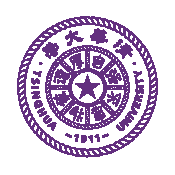
\includegraphics[height=3cm]{thu-fig-logo}}%
  \hspace{4em}%
  \subcaptionbox{第二个小图形,注意这个图略矮些。如果标题很长的话,它会自动换行\label{fig:subfig2}}
      {
\includegraphics[height=2cm]{thu-text-logo}}
  \caption{包含子图形的大图形(subcaptionbox示例)}
  \label{fig:big1-subcaptionbox}
\end{figure}
\begin{figure}[h]
  \centering%
  \begin{subfigure}{3cm}
    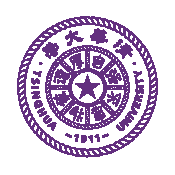
\includegraphics[height=3cm]{thu-fig-logo}
    \caption{第一个小图形}
  \end{subfigure}%
  \hspace{4em}%
  \begin{subfigure}{0.5\textwidth}
    
\includegraphics[height=2cm]{thu-text-logo}
    \caption{第二个小图形,注意这个图略矮些。subfigure中同一行的子图在顶端对齐。}
  \end{subfigure}
  \caption{包含子图形的大图形(subfigure示例)}
  \label{fig:big1-subfigure}
\end{figure}

古之学者必有师。师者,所以传道受业解惑也。人非生而知之者,孰能无惑?惑而不从师,
其为惑也,终不解矣。生乎吾前,其闻道也固先乎吾,吾从而师之;生乎吾後,其闻道也亦
先乎吾,吾从而师之。吾师道也,夫庸知其年之先後生於吾乎!是故无贵无贱无长无少,道
之所存,师之所存也。

嗟乎!师道之不传也久矣,欲人之无惑也难矣。古之圣人,其出人也远矣,犹且从师而问焉;
今之众人,其下圣人也亦远矣,而耻学於师。是故圣益圣,愚益愚。圣人之所以为圣,愚
人之所以为愚,其皆出於此乎?爱其子,择师而教之,於其身也,则耻师焉,惑焉。彼童子
之师,授之书而习其句读者,非吾所谓传其道、解其惑者也。句读之不知,惑之不解,或师
焉,或不焉,小学而大遗,吾未见其明也。巫医、乐师、百工之人不耻相师,  士大夫之族
曰“师”曰“弟子”之云者,则群聚而笑之。问之,则曰:彼与彼年相若也,道相似也,位
卑则足羞,官盛则近谀。呜呼!师道之不复,可知矣。巫医、乐师、百工之人。吾子不齿,
今其智乃反不能及,其可怪也欤!圣人无常师。孔子师郯子、苌子、师襄、老聃。郯子之徒,
其贤不及孔子。孔子曰:“三人行,必有我师。”是故弟子不必不如师,师不必贤於弟子。
闻道有先後,术业有专攻,如是而已。

如果要把编号的两个图形并排,那么小页就非常有用了:
\begin{figure}
\begin{minipage}{0.48\textwidth}
  \centering
  
\includegraphics[height=2cm]{thu-whole-logo}
  \caption{并排第一个图}
  \label{fig:parallel1}
\end{minipage}\hfill
\begin{minipage}{0.48\textwidth}
  \centering
  
\includegraphics[height=2cm]{thu-whole-logo}
  \caption{并排第二个图}
  \label{fig:parallel2}
\end{minipage}
\end{figure}

李氏子蟠,年十七,好古文、六艺,经传皆通习之,不拘於时,学於余。余嘉其能行古
道,作师说以贻之。

\hfill —— 韩愈(唐)

 \chapter{绪论}
 % \documentclass{article}
 % \usepackage{ctex}
 % \usepackage{amsmath}
 % \begin{document}
 % \newtheorem{theorem}{定理}

\section{问题背景}
粘弹性流体广泛存在于日常生活中,粥、冰淇凌、油漆、细胞液等都是粘弹性流体。由于这些流体中存在高分子物质,它们表现出一定的弹性效应。流体在流动中同时表现出粘性和弹性的性质称为粘弹性。材料粘弹性行为的数学模型已经有很长的研究历史\cite{maxwell2013scientific,kelvin1887stability,oldroyd1950formulation,weissenberg1947continuum,zimm1956dynamics,ferry1980viscoelastic,larson1999structure} 。随着近些年来材料科学和生命科学的发展,越来越多的新材料被发现,例如液晶、凝胶、活性物质等\cite{de1975physics,prost2015active,marchetti2013hydrodynamics,ramaswamy2010mechanics,berthier2013non},并且对这些流体粘弹性性质的研究也获得了快速发展\cite{lin2012some,larson1999structure,joseph2013fluid}。

由于实际中的粘弹性流体大多是水溶液,目前大部分模型假设流体不可压缩。然而随着纳米科学等学科的发展,一些粘弹性流体的压缩性变得不可忽略\cite{yu2015compressible,galstyan2015note,chakraborty2015constitutive,pelton2009damping,kim1999numerical,lind2013bubble}。另外,目前大部分模型并没有考虑温度的影响,而实际上粘弹性流体的流动行为与温度密切相关。如何将流体的压缩性和温度纳入粘弹性流体的模型中,是一个具有挑战性的问题\cite{grmela1997dynamicsI,ottinger1997dynamicsII,larson1999structure}。

另外,由于粘弹性效应,粘弹性流体在热力学上处于非平衡态。经典平衡态热力学无法很好地对其进行描述。近些年来随着非平衡态热力学的发展,许多理论被应用于粘弹性流体的建模中\cite{jou1996extended,beris2013thermodynamics,ottinger2005beyond,coleman1961foundations,coleman1964thermodynamics,truesdell2012rational,truesdell2004non,eringen2012microcontinuum,eringen1965theory,zhu2014conservation}。然而,目前大多数理论是从物理原理出发,缺乏数学上对方程适定性的分析。如何建立一个既满足物理原理,又能够满足数学上要求的理论,对于粘弹性流体的数学建模具有重要意义\cite{zhu2014conservation,larson1999structure}。

本文的研究目的,就是推广Zhu、Hong、Yang、Yong提出的非平衡态热力学的守恒-耗散理论,为非等温可压粘弹性流体的建模提供新的手段。利用这些手段本文发展了几类非等温可压粘弹性流体模型并对其进行了数学分析。本文的结果,对于完善守恒-耗散理论、对于粘弹性流体的建模具有重要的意义,所提出的非等温可压粘弹性流体模型,完善了经典的不可压粘弹性流体力学理论。对模型的数学分析是对粘弹性流体进行数学上统一处理的一个尝试,并为粘弹性流体模型的数学分析提供了新的思路。

% 为了研究这些问题,本文考虑的粘弹性流体仅限于简单的高分子溶液。

\section{粘弹性流体建模的研究历程与现状}
对物质粘弹性建模的早期研究出现在19世纪下半叶,Maxwell从阻滞弹簧的模型出发提出了Maxwell线性粘弹性模型\cite{maxwell2013scientific}。经典的Maxwell模型方程如下
\begin{eqnarray*}
\frac {d\epsilon} {dt} = \frac {\sigma} {\eta} + \frac {1} {E} \frac {d\sigma} {dt},
\end{eqnarray*}
其中$\sigma$和$\epsilon$分别为材料的应力张量和应变张量,$\eta$和$E$分别为材料的粘性系数和弹性常数(模量)。在流体中$\frac {d\epsilon} {dt}$一般采用速度梯度量$\nabla v$的对称部分$D=\frac{1}{2} (\nabla v + (\nabla v)^T)$来代替,从而可以得到粘弹性流体的Maxwell模型如下
\begin{equation} \label{eq:maxwell}
			\partial_t \sigma + v \cdot \nabla \sigma - D = -\frac{\sigma}{\xi}. 
\end{equation}
交换上面方程中的应力应变张量得到的模型称为Kelvin-Voigt模型,由物理学家Kelvin和Voigt在19世纪末提出\cite{kelvin1887stability}。

19世纪中叶Weissenberg发现了Weissenberg效应。这一效应是指当转动的杆置于粘弹性流体中时,流体将会沿着杆“爬上”或者“爬下”\cite{weissenberg1947continuum}。为了解释这一效应,Oldroyd提出了粘弹性建模的重要法则:客观性原理。这一原理是说模型不应依赖于坐标系的选取。基于这一原理,他提出了客观导数的概念,并提出了经典的Oldroyd-B模型,这一模型如下
\begin{equation} \label{eq:Oldroyd}
	{\sigma} + \lambda_1 \stackrel{\nabla}{{\sigma}} = 2\eta_0 ({D} + \lambda_2 \stackrel{\nabla}{{D}}).
\end{equation}
其中$\sigma$为应力张量,$\lambda_1$和$\lambda_2$分别为松弛时间和迟滞时间,$\eta_0$为流体的粘性系数,${\stackrel{\nabla} \sigma}= \partial_t \sigma + v \cdot \nabla \sigma - (\nabla v)\  \sigma - \sigma (\nabla v)^T$为$\sigma$的上对流Maxwell导数\cite{oldroyd1950formulation}。Oldroyd的这一论文对粘弹性流体的建模产生了深远的影响。基于这一原理,修改经典Maxwell模型和Kelvin-Voigt模型中的导数为客观导数可以得到许多模型\cite{lin2005hydrodynamics,larson1999structure}。

我们一般将经典的Maxwell等不包含客观导数的模型称为线性粘弹性模型,而将Oldroyd-B等包含客观导数的模型称为非线性粘弹性模型。由上面的方法直接推广的非线性粘弹性模型仅能考虑简单的情况,不能很好地纳入温度的影响。为了解决这些问题,热力学家和力学家提出了许多理论,这些理论主要有两个方向:一是非平衡态热力学理论\cite{jou1996extended,ottinger2005beyond,zhu2014conservation},二是基于热力学原理和有限形变理论的记忆衰减理论\cite{coleman1961foundations,truesdell2012rational}。

\subsection{非平衡态热力学在粘弹性流体建模中的应用}
热力学第二定律告诉我们热力学体系非平衡状态的存在性。为了研究热力学不可逆过程,科学家发展了非平衡态热力学。Onsager在1931和1932年的两篇文章中提出了著名的Onsager倒易关系\cite{onsager1931reciprocal,onsager1931reciprocalII}。由Onsager与Prigogine等人发展的经典非平衡态热力学理论(Classical Irreversible Thermodynamics,简称CIT),自20世纪40年代以来获得了蓬勃发展,并且得到了广泛的承认\cite{jou1996extended,truesdell2012rational}。CIT理论可以将经典的Newton本构关系和Fourier热传导定律纳入其中,然而无法将Maxwell粘弹性模型和Cattaneo热传导模型纳入其理论框架中来。为了推广经典的CIT理论,许多新的非平衡态热力学理论被提出,其中包括理性热力学(Rational Thermodynamics,简称RT)、扩展不可逆热力学(Extended Irreversible Thermodynamics,简称EIT)、非平衡可逆-不可逆一般方程(General Equation for the Non-Equilibrium Reversible-Irreversible Coupling,简称GENERIC)、守恒-耗散理论(Conservation-Dissipation Formalism of irreversible thermodynamics,简称CDF)等\cite{truesdell2012rational,jou1996extended,ottinger2005beyond,zhu2014conservation}。

考虑一般的流体方程
\begin{subequations} \label{eq:fluid}
	\begin{align}
		\partial_t \rho + \nabla \cdot (\rho v) = 0 ,\\
		\partial_t (\rho v) + \nabla \cdot (\rho v \otimes v + P) =  0, \\
		\partial_t[\rho (u + \frac{1}{2} v^2)] + \nabla \cdot [q + \rho (u+\frac{1}{2}v^2) v + P \cdot v] = 0.
	\end{align}
\end{subequations}
其中$\rho,v,u$分别表示流体的密度、速度和内能,$P$表示流体的应力张量。这三个方程分别表示质量守恒、动量守恒和能量守恒。CIT假设平衡态的热力学状态参量仍然可以用来描述非平衡态,并且体系的熵依赖于这些状态变量。这里我们假设体系的比熵(单位质量的熵)为$s=s(\frac{1}{\rho},u)$,利用经典平衡态热力学的Gibbs关系,有
\begin{equation*}
	T ds = du + p d(\frac{1}{\rho}).
\end{equation*}
通过计算可以得到
\begin{equation*}
	\rho \dot{s} = - \frac{1}{T} \nabla \cdot q - \frac{1}{T} P: \nabla v,
\end{equation*}
其中$\dot{s} = \partial_t s + v \cdot \nabla s$表示物质导数。根据热力学第二定律,为保证不可逆过程熵函数的增长,需要$\rho \dot{s} \ge 0 $。根据Onsager倒易关系,热力学流和热力学力之间为线性关系。假设$P$可以分解为$P = p + \pi I + \mathring{P}$,其中$\mathring{P} = P - \frac{1}{3} \mbox{Tr}(P) I$为$P$的无迹部分。根据Onsager倒易关系,我们可以得到下面的本构关系
\begin{eqnarray*}
	q = -\lambda \nabla T, \\
	\pi =  - \zeta \nabla \cdot v, \\
	\mathring{P} = - 2 \eta \mathring{D}.
\end{eqnarray*}
此即热传导的Fourier定律与应力张量的Stokes和Newton本构关系

然而,由于局部平衡假设的存在,CIT仅能描述远离平衡态不远的系统。为了拓展CIT,大部分理论假设非平衡态的描述不仅需要平衡态变量,也需要非平衡态变量。Coleman、Truesdell、Noll等人发展了理性热力学RT。理性热力学理论认为非平衡态不仅依赖于平衡态状态变量,还依赖于状态变量的空间梯度。通过推广Clausius-Duhem不等式,利用Onsager倒易关系得到本构关系。Fourier-Stokes-Newton定律可以由RT理论导出\cite{jou1996extended}。另外,Jou、Lebon等人发展了扩展不可逆热力学EIT。EIT通过拓展非平衡态状态变量,将CIT中的热力学流引入非平衡态状态变量中,来对不可逆过程进行建模。例如我们将$q,\pi,\mathring{P}$引入非平衡态状态变量中,并假设$s = s(\frac{1}{\rho}, u,q,\pi,\mathring{P} )$,则通过计算可以得到熵的产生率为
\begin{equation*}
		\rho \dot{s} = - \frac{1}{T} \nabla \cdot q - \frac{1}{T} P: \nabla v - \alpha_1 \pi \cdot \dot{\pi} - \alpha_2 q \cdot \dot{q} - \alpha_3 \mathring{P} : ({\mathring{P} })^. ,
\end{equation*}
其中$\alpha_1,\alpha_2,\alpha_3$为常数。EIT仍然假设Onsager倒易关系成立,利用Onsager关系,可以得到下面的本构关系。
\begin{subequations} \label{eq:EITconstitutive}
		\begin{align}
	\nabla T^{-1} - \alpha_2 \dot{q} = \mu_1 q - \beta^{''}\nabla \cdot \mathring{P} - \beta' \nabla \pi, \\
	-T^{-1} \nabla \cdot v - \alpha_1 \dot{\pi} = \mu_0 \pi - \beta' \nabla \cdot q , \\
	-T^{-1} \mathring{D} - \alpha_3 (\mathring{P})^. = \mu_2 \mathring{P} - \beta^{''} (\mathring{\nabla q})^s,
		\end{align}
\end{subequations}
其中$A^s = \frac{1}{2} (A+A^T)$表示张量$A$的对称部分。通过取合适的参数可以得到Maxwell-Cattaneo定律。
\begin{eqnarray*}
	\tau_1 \dot{q} + q = - \lambda \nabla T, \\
 	\tau_0 \dot{\pi } + \pi = -\zeta \nabla \cdot v, \\
 	\tau_2 (\mathring{P})^. + \mathring{P} = -2 \eta \mathring{D}.
\end{eqnarray*}
其中$\sigma = \pi I + \mathring{P}$。对于不可压流体,我们可以得到Maxwell模型。EIT可以很好地用于线性粘弹性流体模型,然而对于含客观导数的非线性粘弹性本构关系,缺乏简单的处理方式\cite{jou1996extended}。

为了处理复杂的非线性粘弹性流体模型,Beris和Edwards等人通过拓展经典力学的Hamilton理论,在Possion括号之外引入耗散括号(dissipative bracket)来描述能量的耗散和不可逆过程熵的增长\cite{edwards1990remarks,beris2013thermodynamics}。假设$X$为非平衡态系统的状态变量,系统的广义Hamilton函数设为$H=H(X)$,则$X$的演化方程为
\begin{equation*}
	\frac{dX}{dt} = L(X) \cdot \frac{\delta H(X)}{\delta X} + M(X) \cdot \frac{\delta H(X)}{\delta X}, 
\end{equation*}
其中$L=L(x)$和$M=M(x)$为体系的Possion矩阵和耗散矩阵。这一理论通过给出系统的能量和熵函数,并选取合适的$L$和$M$而得到描述体系的方程。 为了满足能量守恒和熵增原理,我们假设$L$与$M$可以定义Possion括号和耗散括号
\begin{equation*}
	\{ A,B \} = \frac{\delta A(X)}{\delta X} \cdot L(X) \cdot \frac{\delta B(X)}{\delta X}, \quad  [ A,B ] = \frac{\delta A(X)}{\delta X} \cdot M(X) \cdot \frac{\delta B(X)}{\delta X}. 
\end{equation*}
其中$L$的选取需要满足经典的Possion括号定义,$M$的选取使得下面的条件成立
\begin{equation*}
	[\int \rho(x) dx, H]=0,[\int \rho(x) v(x) dx, H]=0, \quad [E,H] = 0,
\end{equation*}
以及
\begin{equation*}
	[S,H] \ge 0,
\end{equation*}
由此可知守恒率和热力学第二定律成立。对于不可压粘弹性流体,我们忽略温度的影响,则可以取状态变量$X= 
 \{v,c\}$,其中张量$c$表示非平衡态变量(与粘弹性引起的应变能耗散有关)。取Hamilton量为
 \begin{equation*}
 	H = \int \frac{1}{2} v^2(x) + \frac{1}{2} \mbox{
 	Tr}(c(x))- \frac{1}{2}  \ln \det c(x) dx,
 \end{equation*}
以及Possion矩阵和耗散矩阵为
\begin{equation*}
	L = \left( \begin{array}{cc} 
			u \cdot \nabla &  L_{12} \\
			L_{21}& 0
		\end{array}\right), \quad
	M =	\left( \begin{array}{cc} 
			0  & 0 \\
			0  & c \otimes I
		\end{array}\right),
\end{equation*}
其中
\begin{eqnarray*}
	(L_{12})_{l,kj} = - \frac{\partial}{\partial x_m} c_{mk} \delta_{jl} -  \frac{\partial}{\partial x_m} c_{jm} \delta_{kl}, \\
	(L_{21})_{jk,l} = -c_{mk} \delta_{jl} \frac{\partial}{\partial x_m} - c_{jm} \delta_{kl} \frac{\partial}{\partial x_m}.
\end{eqnarray*}
这里$m$对$1$到$n$求和,$n$为空间维数。本文中如无特别说明,我们采用Einstein求和约定,相同的指标表示求和。
取能量和熵函数为
\begin{equation*}
	E = \int \frac{1}{2} v^2(x)dx, \quad S = -\int \frac{1}{2} \mbox{
 	Tr}(c(x))- \frac{1}{2}  \ln \det c(x) dx.
\end{equation*}
我们可以得到下面的上对流Maxwell模型
\begin{subequations}\label{eq:chap1UCMmaxll}
\begin{align}
	v_t + v \cdot \nabla v + \nabla p  - \nabla \cdot (c - I) = 0, \\
	c_t + v \cdot \nabla c - (\nabla v)c - c (\nabla v)^T = -\frac{c-I}{\lambda}.
\end{align}
\end{subequations}

由于Beris和Edwards理论对耗散括号要求的复杂性,如何提出满足要求的耗散矩阵是一个很有挑战性的问题。为了解决这一问题,\"Ottinger与Grmela发展了GENERIC理论\cite{ottinger2005beyond}。GENERIC并不假设非平衡态Hamilton函数的存在,而是仅仅假设能量和熵的存在性。假设$X$为非平衡态系统的状态变量,其演化方程可以写为
\begin{equation*}
	\frac{dX}{dt} = L(X) \cdot \frac{\delta E(X)}{\delta X} + M(X) \cdot \frac{\delta S(X)}{\delta X} ,
\end{equation*}
其中$E=E(X)$和$S=S(X)$分别为系统的能量和熵,$L=L(x)$和$M=M(x)$为体系的Possion矩阵和耗散矩阵。GENERIC通过给出系统的能量和熵函数,选取合适的$L$和$M$即可得到描述体系的方程。 为了满足能量守恒和熵增原理,我们假设$L$与$M$可以定义Possion括号和耗散括号
\begin{equation*}
	\{ A,B \} = \frac{\delta A(X)}{\delta X} \cdot L(X) \cdot \frac{\delta B(X)}{\delta X}, \quad  [ A,B ] = \frac{\delta A(X)}{\delta X} \cdot M(X) \cdot \frac{\delta B(X)}{\delta X}. 
\end{equation*}
其中$L$的选取需要满足经典的Possion括号定义,$M$的选取使得下面的条件成立
\begin{equation*}
	[A,B] = [B,A], \quad [A,A] \ge 0.
\end{equation*}
假设系统的能量为$E$,熵函数为$S$,我们假设$L,M$满足下面的退化条件
\begin{equation}
	L \frac{\delta S}{\delta X} = 0, \quad M \frac{\delta E}{\delta X} = 0,
\end{equation}
那么任意泛函$A$的演化方程为
 \begin{equation*}
	\frac{d A}{dt} = \frac{\delta A(x)}{\delta x} \cdot \frac{dx}{dt} = \{ A,E\} + [A,S].
\end{equation*}
于是可以得到
\begin{eqnarray*}
	\frac{d E}{dt} = \{E,E\} +[S,E] = 0, \\
	\frac{d S}{dt} = [S,S] \ge 0. 
\end{eqnarray*}
这里我们用到了退化条件$[E,S] = 0$。在GENERIC中关键的是选取合适的Possion矩阵和耗散矩阵,使之满足Possion括号和耗散括号的定义以及退化条件。GENERIC将物理量的演化分成了两个部分,一部分是由可逆过程引起的,而另一部分是由不可逆过程引起的,具体通过Possion括号和耗散括号实现,并且与退化条件一起保证了热力学第一定律和第二定律的成立。然而在上面上对流Maxwell模型的例子中,却很难将可逆过程和不可逆过程的影响通过这种方式分开,如果我们采用上面的能量和熵函数$E,S$,以及矩阵$L,M$,那么可以验证$L$不满足退化条件。  

由于EIT缺乏对含客观导数的非线性粘弹性模型的考虑,Beris-Edwards中Possion矩阵和耗散矩阵选取的复杂性以及GENERIC对可逆部分和不可逆部分耦合方式的简单性,这些理论都没有完美地解决粘弹性流体的建模问题。另一方面,这些理论建立在物理定律的基础上,缺乏对方程数学性质的分析。除上面提到的非平衡态热力学理论之外,也有很多其他的非平衡态热力学理论试图解决粘弹性流体的建模问题,可以参看\cite{stratonovich2012nonlinear,huo1993nonequilibrium,eu1992kinetic}。

基于Yong的双曲方程守恒-耗散结构条件\cite{yong2008interesting},Zhu、Hong、Yang、Yong发展了不可逆热力学的守恒-耗散理论(CDF)\cite{zhu2014conservation}。Yong等发展的守恒-耗散理论(以下简称守恒-耗散理论)通过守恒-耗散结构条件保证了热力学第一定律和第二定律的成立,并且得到的方程组满足Yong的稳定性条件,从而有着良好的数学性质\cite{yong1992singular}。守恒-耗散理论已经顺利地应用于线性粘弹性流体力学模型\cite{zhu2014conservation}。然而,由于目前的守恒-耗散理论考虑的是守恒形式的方程,而客观导数的存在将会导致方程不再可以写成守恒形式,所以守恒-耗散理论在应用到非线性粘弹性流体模型时遇到了困难。本文将推广这一理论并将其应用于非线性粘弹性流体的建模中。

\subsection{粘弹性流体的记忆衰减理论}
由于粘弹性流体可以看作连续介质,所以可以采用连续介质力学的理论对其进行建模。前文提到的模型一般都是通过小变形连续介质力学得到的,而对于粘弹性流体来说,尤其是高弹性的流体,小形变假设不再适用。基于此,Coleman和Noll等人提出了利用有限形变理论对粘弹性流体进行建模的方法\cite{coleman1961foundations,coleman1964thermodynamics,coleman2012viscometric}。该理论认为物质的状态依赖于其形变的历史,而形变可以用形变张量$F$来描述。这里$F$定义为流动图$x = x(X,t)$的梯度$F_{ij} = \frac{\partial x_i}{\partial X_j}$,其中$x,X$分别对应于流体质点的Euler和Lagrange坐标。根据定义可以得到
\begin{equation}\label{eq:Feq}
	\partial_t F + v \cdot \nabla F = (\nabla v) F.
\end{equation}
这一理论认为应力张量是$F$的历史和温度$\theta$的历史的函数。假设体系的自由能为
\begin{equation*}
	\psi = \mathop{\psi} \limits_{\tau=0}^{t}( C(t), C^t(\tau),\theta(t),\theta^t(\tau)).
\end{equation*}
其中$C(t) = F^T(t) F(t),C^t(\tau) = C(t - \tau)$。$\psi$依赖于从初始时刻到当前时刻$t$的应变历史。利用Gibbs关系,可以得到
\begin{equation}\label{eq:en}
	\rho \frac{d\psi}{dt} + \rho \eta \frac{d \theta}{dt} - T: \frac{dC}{dt} + w = 0.
\end{equation}
其中$T$代表第二Piola-Kirchhoff张量,与Cauchy应力张量$\sigma$的关系为$\sigma = \rho F T F^T$,$w$代表能量的耗散。由$\psi$的表达式可以得到
\begin{equation*}
	\frac{d\psi}{dt} = \frac{\partial \psi}{\partial C} : \frac{d C}{dt}+ \frac{\partial \psi}{\partial \theta} \frac{d\theta}{dt} + \delta \psi.
\end{equation*}
代入\eqref{eq:en}中得到
\begin{equation*}
	(\rho \frac{\partial \psi}{\partial C} - T) : \frac{dC}{dt} + \rho (\frac{\partial \psi}{\partial \theta} + \eta) d\theta + (w + \rho \delta \psi) dt  =0.
\end{equation*}
从而得到
\begin{eqnarray*}
	T = \rho \frac{\partial \psi}{\partial C} = \mathop{\mathcal{F}}\limits_{\tau=0}^{t} ( C(t), C^t(\tau),\theta(t),\theta^t(\tau)), \\
	\eta = -\frac{\partial \psi}{\partial \theta},\\
	w = -\rho \delta \psi.
\end{eqnarray*}
热力学第二定律由$w \ge 0$保证\cite{coleman1961foundations,dimitrienko2010nonlinear}。

例如经典的上对流Maxwell模型的熵函数可以取作(忽略温度)
\begin{equation*}
	\psi  = \psi(t) = - \frac{1}{\lambda}  \ln \det (F^T(t) F(t)) + F^T(t) F(t) : \frac{1}{\lambda}  \int_{0}^t e^{-\frac{t-s}{\tau}} F^{-1}(\tau) F^{-T}(\tau) d\tau,
\end{equation*}
于是有
\begin{equation*}
	T = \frac{1}{\lambda}  \int_{0}^t e^{-\frac{t-s}{\tau}} F^{-1}(\tau) F^{-T}(\tau) d\tau -\frac{1}{\lambda}  F^{-1} F^{-T} .
\end{equation*}
应力张量$\sigma$可以写为
\begin{equation*}
	\sigma = \frac{1}{\lambda} \int_{0}^{t} e^{-\frac{(t-s)}{\lambda} } F(t)  F^{-1}(s) F^{-T}(s) F^T(t)  dx.
\end{equation*}
注意上面的积分是沿流线的积分。于是根据\eqref{eq:Feq},可以得出$\sigma$满足上对流Maxwell模型,该模型的能量耗散为
\begin{equation*}
	w = - \rho \frac{1}{\lambda} \mbox{Tr}(I) = -\frac{3\rho}{\lambda} < 0.
\end{equation*}
这违背了热力学第二定律对$w>0$的要求。所以这一理论不能很好地包括上对流Maxwell模型。


另外,Lin、Liu、Zhang在文献\cite{lin2005hydrodynamics}中提出了下面的模型
\begin{subequations}\label{eq:linincompressible}
	\begin{align}
		\nabla \cdot v = 0, \\
		v_t + v \cdot \nabla v + \nabla p = \mu \Delta v + \nabla \cdot( F F^T), \\
		F_t + v \cdot \nabla F = \nabla v F.
	\end{align}
\end{subequations}
Lei、Liu、Zhou在\cite{lei2008global}中发展这一方程组至可压缩形式。可压形式的方程组如下
\begin{subequations}\label{eq:lincompressible}
	\begin{align}
		\rho_t + \nabla \cdot (\rho v) = 0, \\
		(\rho v)_t + \nabla \cdot (\rho v \otimes v) + \nabla p = \mu \Delta v + \mu' \nabla \nabla \cdot v+ \nabla \cdot( \rho F F^T), \\
		F_t + v \cdot \nabla F = \nabla v F.
	\end{align}
\end{subequations}
这一模型实际上对应于无穷大Weissenberg数Oldroyd模型\cite{lei2008global},以下简称这一模型为Lin等人的模型。这里的模型实际上是Navier-Stokes方程的一个推广,利用有限形变理论将弹性形变$\rho F F^T$包含在了应力张量之中。这一模型因为有着良好的数学结构而得到了许多数学上好的结果\cite{lin2012some},但是尚缺乏在实际中的应用实例。

综上所述,有限形变理论是一个描述连续介质力学的很好工具。利用有限形变理论,结合非平衡态热力学的方法发展起来的热力学理论在粘弹性流体的建模方面有一定的优势,但是也存在一些问题。

本论文将讨论基于守恒-耗散理论和有限形变理论的粘弹性流体建模方法。

\section{粘弹性流体的数学分析}
由于粘弹性流体方程的重要性和复杂性,其数学分析一直以来都吸引了很多数学家的兴趣\cite{lin2012some,li2007mathematical,weinan2002convergence,fabrizio1992mathematical,renardy2008mathematical,joseph1987hyperbolicity,guillope2010regular,saut2012lectures,yong2014newtonian,qian2010well,hu2011global,lei2005global,fang2014incompressible}。目前的分析主要集中于不可压方程,主要包括Oldroyd-B模型、上对流Maxwell模型、FENE模型、以及Lin等人的模型\cite{elgindi2015global,saut2012lectures,renardy2000mathematical,masmoudi2011global,lions2000global,masmoudi2008well,lei2010remarks}。近些年来,也有部分工作讨论了可压粘弹性流体方程\cite{fang2014incompressible,hu2012strong,qian2010global,qian2011initial}。
\subsection{经典粘弹性流体力学模型的数学分析}
经典的粘弹性流体模型主要包括线性粘弹性流体力学模型Maxwell模型\eqref{eq:maxwell}和Kelvin-Voigt模型,以及非线性粘弹性流体模型上对流Maxwell模型\eqref{eq:chap1UCMmaxll}、Oldroyd-B模型\eqref{eq:Oldroyd}和采用其他客观导数的类似模型等。对这些方程的分析主要集中于方程弱解的全局存在性、光滑解的局部存在性、平衡态附近解的整体存在性,以及松弛参数(通常为Weissenberg数)趋于$0$时的极限分析。我们这里只考虑宏观模型,对于微观模型的数学结果可以参看Masmoudi、Li、Zhang、E、Sun等人的工作\cite{masmoudi2013global,masmoudi2008well,li2007mathematical,li2004local,li2004well,lions2007global,weinan2002convergence,constantin2010remarks}。

对于线性粘弹性流体的分析结果可以参看\cite{fabrizio1992mathematical,renardy2000mathematical}。书中对线性粘弹性的数学结果做了总结,主要讨论并证明了方程解的存在性和唯一性、稳定性和稳态方程解的存在性和唯一性。由于线性粘弹性流体的适用范围的局限性,大部分分析工作均围绕非线性粘弹性流体模型。最简单的非线性粘弹性流体模型是对流导数Maxwell模型和Oldroyd模型。首先我们考虑对流导数的Maxwell模型
\begin{subequations}\label{eq:Oldroyda}
\begin{align}
	\lambda \frac{\mathcal{D}_a \sigma}{\mathcal{D} t} + \sigma = 2 \eta D, \\
	\partial_t v + v \cdot \nabla v  + \nabla p = \nabla \cdot \sigma, \\
	\nabla \cdot v = 0,
\end{align}
\end{subequations}
其中
\begin{equation*}%\label{eq:convectderivative}
	\frac{\mathcal{D}_a \sigma}{\mathcal{D} t} = \partial_t \sigma + v \cdot \nabla \sigma + \sigma W- W \sigma - a(D \sigma + \sigma D), \ W = \frac{1}{2}(\nabla v - (\nabla v)^T).
\end{equation*}
当$a=1$时\eqref{eq:Oldroyda}为上对流Maxwell模型\eqref{eq:chap1UCMmaxll},$a=-1,0$分别对应于Jaumann和下对流导数Maxwell模型。针对方程组\eqref{eq:Oldroyda},Rutkevich等人对其双曲性进行了分析\cite{rutkevich1969some,rutkevich1970propagation},Joseph、Saut、Renardy等人发展了Rutkevich的结果\cite{joseph1987hyperbolicity,joseph1986change}。由这些工作,可以得到方程组\eqref{eq:Oldroyda}在下面的条件下会出现Hadamard不稳定性:
\begin{equation*}
	\frac{1-a}{2} \Lambda_M - \frac{1+a}{2} \Lambda_m > \frac{\eta}{\lambda}.
\end{equation*}
其中$\Lambda_M$和$\Lambda_m$分别为$\sigma$的最大和最小特征值。根据这一分析,可以得到不稳定性仅可能在$a\in (-1,1)$时发生。对于上对流和下对流导数(分别对应于$a=-1$和$1$),模型\eqref{eq:Oldroyda}是双曲的,不会出现Hadamard不稳定性。
% 另外Joseph、Saut、Renardy等人还对稳态方程的双曲性进行了分析。
另外对该模型解的存在性结果可以参看\cite{saut2012lectures}。

由于Oldroyd模型的广泛应用和重要性,大部分数学工作都是围绕这一方程进行的。这一模型的一般方程为
\begin{subequations}\label{eq:Oldroydb}
\begin{align}
	\lambda \frac{\mathcal{D}_a \sigma}{\mathcal{D} t} + \sigma = 2 \eta_p D, \\
	\partial_t v + v \cdot \nabla v  + \nabla p = \nabla \cdot \sigma + 2 \eta_s \Delta v, \\
	\nabla \cdot v = 0.
\end{align}
\end{subequations}
其中$\eta_s,\eta_p$分别为溶剂和溶质的粘性系数。这一模型与对流导数Maxwell模型\eqref{eq:Oldroyda}的区别是在动量方程中添加了溶剂粘性$2\eta_s \Delta v$一项。
下面我们将讨论这一模型的主要数学结果。首先其解的局部存在性定理由Guillope、Saut等人在\cite{guillope1990existence}给出。证明主要采用了包含时间的Stokes问题的解的存在性结果\cite{temam1995navier},并利用了Sobolev演算不等式\cite{majda2012compressible}和经典的不动点理论。例如对于\eqref{eq:Oldroydb}中$\sigma$的估计,$\sigma$的方程两端与$\sigma$做内积可以得到
\begin{equation*}
	\frac{d}{dt} \|\sigma\|_{L^2}^2  =  -\frac{1}{\lambda} \|\sigma\|_{L^2}^2 + 2 (\frac{\eta}{\lambda} D, \sigma) + \left( (a(D \sigma + \sigma D) - (\sigma W -W \sigma)),\sigma \right).
\end{equation*}
右端第二项可以利用H\"older不等式估计如下
\begin{equation*}
	(\frac{\eta}{\lambda} D, \sigma) \le \frac{\eta}{\lambda} \|\sigma\|_{L^2} \|\nabla v\|_{L^2}.
\end{equation*}
第三项可以估计为
\begin{equation*}
	 \left( (a(D \sigma + \sigma D) - (\sigma W -W \sigma)),\sigma \right) 
%\le \|\sigma\|_{L^2}^2 \|\nabla v\|_{L^\infty} 
\le \|\sigma\|^2_{L^2} \|\nabla v\|_{H^2}
.
\end{equation*}
上式中最后一个不等号由Sobolev嵌入定理得到。为了估计$\|\nabla v\|_{H^2}$,需要对$v$的方程估计,最终可以得到\cite{guillope1990existence}
\begin{equation*}
		\frac{d}{dt} \|\sigma\|_{H^2}^2 + \frac{1}{\lambda} \|\sigma\|_{H^2}^2 \le C \frac{\eta}{\lambda} \|v\|_{H^3} \|\sigma\|_{H^2} + C \|v\|_{H^3} \|\sigma\|_{H^2}^2.
\end{equation*}
从而得到$\sigma \in L^\infty([0,T],H^2)$。然后利用Stokes问题的结论,最终可以证明下面的局部存在性定理:
\begin{theorem}(Guillope,Saut等\cite{guillope1990existence,saut2012lectures})
	假设$\sigma_0 \in H^2(\mathbf{R}^3),v_0 \in D(A)$,$D(A)$为$L^2$上Stokes算子的定义域。那么存在时间$T>0$,使得方程组\eqref{eq:Oldroydb}存在唯一的光滑解$(v,p,\sigma)$,且满足
	\begin{equation*}
		v \in L^2([0,T],H^3) \cap C([0,T],D(A)), \ p \in L^2([0,T],H^2) \ \sigma \in C([0,T],H^2).
	\end{equation*}
\end{theorem}
方程\eqref{eq:Oldroydb}的平衡点$(v=0,\sigma=0)$附近解的整体存在性首先由文献\cite{guillope1990existence}给出,其中假设了$\eta_s/\eta_p$足够大。这一假设是为了保证粘性项$ 2 \eta_s \Delta v$的耗散足够好从而使得$\sigma$的范数可以被$v$的范数控制。采用不同的方法,这一假设被移除,更一般的整体存在性结果也已经被证明\cite{chupin2004some,molinet2004global,molinet2004existence}。Molinet等人采用了$\|\mathcal{P}\nabla \cdot \sigma\|_{H^1}$来代替文献\cite{guillope1990existence}中的$\|\nabla \cdot \sigma\|_{H^1}$估计,从而得到更好的结果如下\cite{molinet2004global,molinet2004existence}:
\begin{theorem}(Molinet等\cite{molinet2004existence})
	假设$\sigma_0 \in H^2(\mathbf{R}^3),v_0 \in D(A)$足够小,那么方程组\eqref{eq:Oldroydb}在$t\in [0,\infty)$上存在唯一的光滑解$(v,p,\sigma)$,且满足
	\begin{eqnarray*}
		v \in L^2([0,\infty],H^3) \cap C([0,\infty],D(A)), \ p \in L^2([0,\infty],H^2), \ \sigma \in C([0,\infty],H^2).
	\end{eqnarray*}
\end{theorem}

在$L^p$框架下方程组\eqref{eq:Oldroydb}解的存在性证明可以参见Fernandez、Zhang和Fang的工作\cite{fernandez1998some,zhang2012global}。Besov空间的存在性结果见Chemin和Masmoudi的工作\cite{chemin2001lifespan}。

对于方程组\eqref{eq:Oldroydb}的弱解的整体存在性,Constantin和Sun证明了空间$C^\alpha(\mathbf{R}^n) \cap L^1(\mathbf{R}^n)$中弱解的存在性\cite{constantin2010remarks,saut2012lectures}。对于$a=0$的情况,$L^2$意义下弱解的整体存在性被Lions和Masmoudi证明\cite{lions2000global}。这一证明利用了对于$a=0$的模型,方程组\eqref{eq:Oldroydb}中$\sigma$成立下面的估计
\begin{equation*}
	\frac{d}{dt} \left(\frac{1}{2} \|v\|_{L^2}^2 +  \frac{\lambda}{4 \eta_p} \|\sigma\|_{L^2}^2 \right) + \frac{1}{2\eta_p} \|\sigma\|_{L^2}^2 + {2 \eta_s} \|\nabla v\|_{L^2}^2 = 0,
\end{equation*}
然而由于对于一般的情况,这一估计并不成立,弱解的存在性也尚未得到证明\cite{saut2012lectures}。

另外一个重要的数学问题为$\lambda$趋于$0$时方程组\eqref{eq:Oldroydb}的极限分析。形式上$\lambda$为$0$时我们得到Navier-Stokes方程组,即Newton流体模型。这一问题也经常被称为Newton极限问题。我们将$\sigma$的方程写成下面的形式
\begin{equation*}
	 \sigma = -	\lambda \frac{\mathcal{D}_a \sigma}{\mathcal{D} t} +  2 \eta_p D.
\end{equation*}
$\lambda=0$时,$\sigma= 2 \eta_p D$,从而方程组\eqref{eq:Oldroydb}成为经典的不可压Navier-Stokes方程组:
\begin{subequations} \label{eq:innavierstokes}
\begin{align}
	\partial_t v + v \cdot \nabla v  + \nabla p &= \nabla \cdot \sigma + 2 \eta \Delta v, \\
	\nabla \cdot v &= 0.
\end{align}
\end{subequations}
其中$\eta= \eta_s + \eta_p$。Molinet和Talhouk基于Fourier分析,通过对低频和高频情况的分析,得到了\eqref{eq:Oldroydb}和上面的Navier-Stokes方程组\eqref{eq:innavierstokes}兼容性的分析。证明了下面的定理:
\begin{theorem}(Monlinet和Talhouk\cite{molinet2008newtonian})
	令$n=2,3$,$(v_0,\sigma_0) \in H^s(\mathbf{R}^n) \times H^s(\mathbf{R}^{n^2}), s>\frac{n}{2}$。假设$v$为方程组\eqref{eq:innavierstokes}以$v_0$为初值的解,在$[0,T_0],T_0>0$上存在且$v \in C([0,T_0],H^s)$。那么对于任意的$\delta \in (0,1)$,存在
	\begin{equation*}
		\varepsilon_0 = \varepsilon_0 (n,\lambda,\eta_p,\eta_s,\delta, \|v\|_{{L_{T_0}^\infty}H^s}, \|\nabla v\|_{{L^2_{T_0}}H^s}, \|\sigma_0\|_{H^s}) >0,
	\end{equation*}
	使得对任意的$0 < \lambda < \varepsilon_0$,满足$0 < \frac{\eta_p}{\eta} \le 1- \delta$的方程组\eqref{eq:Oldroydb}存在唯一解
	\begin{equation*}
		v_\lambda \in C([0,T_0],H^s),\ \nabla v_{\lambda} \in L^2([0,T_0],H^s), \ \sigma_{\lambda} \in C ([0,T_0],H^s),
	\end{equation*}
	且当$\lambda \rightarrow 0$时,成立
	\begin{eqnarray*}
		v_\lambda \rightarrow v \quad \text{在} C([0,T_0],H^s) \text{中}, \\ 
		\sigma_\lambda - 2\eta_p D[v_\lambda]  \rightarrow v \quad \text{在} L^2([0,T_0],H^s) \text{中}, \\ 
		\lambda^{\frac{1}{2}} \sigma_\lambda \rightarrow v \quad \text{在} C([0,T_0],H^s) \text{中}.
	\end{eqnarray*}
\end{theorem}
这样对于$\eta_s \neq 0, \eta_p \neq 0$的情况,方程组\eqref{eq:Oldroydb}和Navier-Stokes方程组\eqref{eq:innavierstokes}的兼容性得到了严格地分析。另外,对于弱解下的Newton极限的分析,可以参看\cite{bresch2014newtonian}。


近些年来,一些可压缩粘弹性流体力学模型的数学分析开始吸引一些数学家的兴趣,主要集中于推广的Oldroyd模型。Bollada和Phillips总结了关于可压粘弹性模型的数学建模工作\cite{bollada2012mathematical},并利用Lie导数和微分几何导出了可压上对流Maxwell模型。关于这些模型的分析工作目前主要集中于局部存在性和平衡态附近的整体存在性的证明以及不可压极限的分析\cite{zhang2012global,fang2013strong,fang2014incompressible,matuvsuu1999existence,fang2013strong,barrett2016existence,salloum2011local}。例如,Fang和Zi等\cite{fang2013strong}给出了下面的可压Oldroyd-B模型
\begin{subequations}
	\begin{align*}
	\rho_t + \nabla \cdot (\rho v) = 0. \\
	(\rho v)_t + \nabla \cdot (\rho v \otimes v)  + \nabla p = \nabla \cdot \sigma + 2 \eta_s \Delta v, \\
	\lambda \frac{\mathcal{D}_a \sigma}{\mathcal{D} t} + \sigma = 2 \eta_p D
	\end{align*}
\end{subequations}
的局部存在性结果。其不可压极限为\eqref{eq:Oldroydb}的分析在\cite{fang2014incompressible}给出。

另外,也有许多关于其他模型的数学分析工作,例如FENE模型\cite{masmoudi2008well,zhang2006local,jourdain2004existence,liu2008boundary}、Giesekus模型\cite{renardy1984existence}等等。

\subsection{Lin等人的模型的数学分析}
由于Lin等人的模型有着良好的数学结构,其吸引了许多数学家的兴趣\cite{lin2005hydrodynamics,lebon2008classical,qian2010well,qian2011initial,hu2012formation,hu2015global}。在\cite{lin2005hydrodynamics}中,该方程在二维的Cauchy问题的局部存在性和在平衡态附近的整体存在性均得到了证明。证明基于力学上的适应性条件$\nabla \cdot F^T=0$,由此可以找到势函数$\phi$,使得$F = \nabla \times \phi$,在二维时
\begin{equation*}
	F = \left( \begin{matrix}
		-\partial_{x_2} \phi_1 & -\partial_{x_2} \phi_2 \\
		\partial_{x_1} \phi_1 & \partial_{x_1} \phi_2
	\end{matrix}\right).
\end{equation*}
于是方程组\eqref{eq:linincompressible}可以写为下面的形式
\begin{eqnarray*}
	\nabla \cdot v = 0, \\
	v_t + v \cdot \nabla v + \nabla p =  \mu \Delta v - \sum_{i=1}^2 \Delta \phi_i \nabla \phi_i, \\
	\phi_t + v \cdot \nabla \phi = 0.
\end{eqnarray*}
利用Galerkin逼近,其解的局部存在性可以得到证明\cite{lin2005hydrodynamics},证明过程采用了Gagliardo–Nirenberg插值不等式
\begin{equation*}
	\|v\|_{L^4}^2 \le C \|v\|_{L^2} \| \nabla v\|_{L^2} ,\ \|\nabla \phi\|_{L^4}^2 \le C \|\nabla \phi\|_{L^2}^{3/2} \|\nabla \Delta \phi\|_{L^2}^{1/2}.
\end{equation*}
利用基本的能量估计和上面的不等式,对高阶导数进行估计,可以得到下面的存在性定理:
\begin{theorem}(Lin、Liu、Zhang\cite{lin2005hydrodynamics})
	令$s \ge 2$,$\nabla \phi_0 \in H^s(\mathbf{R}^2),v_0 \in H^s(\mathbf{R}^2)$。那么存在仅仅依赖于$\|\nabla \phi_0\|_{H^2}$和$\|v_0\|_{H^2}$的时间$T>0$,使得方程\eqref{eq:linincompressible}在时间区间$[0,T]$上存在唯一解$U=(v,F=\nabla \phi) \in C([0,T],H^s) \cap C([0,T],H^{s+1})$。且如果解的最大存在时间为$T^*$,那么
	\begin{equation*}
		\int_0^{T^*} \|\nabla v\|_{H^2}^2 ds = + \infty.
	\end{equation*}
\end{theorem}

为了分析方程\eqref{eq:linincompressible}在二维时解在平衡态附近的整体存在性。取$\psi(x) = \phi(x)-x$,并令$w=v-\frac{1}{\mu}\psi$,而将方程组\eqref{eq:linincompressible}写成下面的形式
\begin{eqnarray*}
	\nabla \cdot v =0 , \\
	w_t - \mu \Delta w = - v \cdot \nabla w - \nabla p = - \Delta \psi \nabla \psi + \frac{v}{\mu}, \\
	\psi_t + v \cdot \nabla \psi = -v.
\end{eqnarray*}
这样一来在平衡态附近$w$由于右端项$-v$的衰减效应,以及$w$方程的抛物效应,该方程的整体解存在,下面的定理成立:
\begin{theorem}(Lin、Liu、Zhang\cite{lin2005hydrodynamics})
	令$s \ge 2$,$\nabla \phi_0 \in H^s(\mathbf{R}^2),\det(\phi_0) = 1, v_0 \in H^s(\mathbf{R}^2)$。那么对于足够小的$\|\nabla \psi_0\|_{H^2}$和$\|v_0\|_{H^2}$,方程\eqref{eq:linincompressible}存在唯一的整体光滑解$U=(v,F-I=\nabla \psi) \in C([0,\infty],H^s)$,且满足
	\begin{equation*}
		\|v\|_{H^2}^2 +\|\nabla \psi\|_{H^2}^2 + \int_0^\infty \|\nabla v\|_{H^2}
^2ds \le C \|\nabla \psi_0\|_{H^2} + \|v_0\|_{H^2}.
	\end{equation*}
	\end{theorem}
	在二维的情形,证明中利用了力学上的适应性条件$\nabla \cdot F^T = 0$和$\det F =1$。其中第一个条件保证了势函数$\phi$的存在,第二个条件保证了$\nabla \cdot \psi$充分小,从而可以得到整体存在性定理。
对于三维的情形,Lei等人在\cite{lei2008global}中证明了其解的局部存在性和整体存在性。其局部存在性证明方法与\cite{lin2005hydrodynamics}类似,但是采用了三维情况下的Gagliardo–Nirenberg插值不等式。对于整体解存在性的证明,其采用了$E=F-I$的适应性条件$E_{lj}\partial_{x_l} E_{ik}=E_{lk}\partial_{x_l} E_{ij}$以及$\nabla \cdot F^T=\nabla \cdot E^T=0$。
%从而$\Delta E$可以采用Hodge分解得到
% \begin{equation*}
% 	\Delta E = \nabla \nabla \cdot E^T -  \nabla \time \nabla E.
% \end{equation*}
% 于是成立下面的估计
% \begin{equation*}
% 	\|\Delta E\|^2_{L^2} \le C \|E\|_{H^2}^2 \|\Delta E\|_{L^2}^2.
% \end{equation*}
% 于是$E$很小时可以得到$\|\Delta E\|^2_{L^2}$有界,从而可以得到整体存在性定理的证明\cite{lin2005hydrodynamics}。

另外,这一模型还可以推广到可压缩模型\eqref{eq:lincompressible}。其可压缩模型的局部存在性和平衡态附近解的整体存在性定理的证明可以参看Qian、Zhang、Hu、Wang等人的工作\cite{qian2010global,hu2011global,hu2012strong}等。其中的证明采用了Besov空间,并利用了Danchine等关于Navier-Stokes小解整体存在性的证明思路和方法\cite{danchin2000global},且很好地利用了力学上的适应性条件。例如\cite{qian2010global}中考虑平衡点$\rho=\rho_e,v=0,F=I$附近解的存在性,通过定义
\begin{equation*}
	d:=\Lambda^{-1} \nabla \cdot v, \ e:= \Lambda^{-1} \nabla v, \ \Lambda :=(-\Delta)^{-\frac{1}{2}},
\end{equation*}
以及
\begin{equation*}
	E=F-I, \ \sigma = \frac{\gamma}{\rho_e} (\rho - \rho_e), \ \gamma = (p_{\rho}(\rho_e))^{1/2},
\end{equation*}
可以将方程\eqref{eq:lincompressible}写成下面的双曲-抛物方程组
\begin{eqnarray*}
	\sigma_t + v \cdot \nabla \sigma + \gamma \Lambda d = G_1, \\
	e_t + v \cdot \nabla e - \mu \Delta e - \mu' \nabla \nabla d + \gamma \Lambda^{-1} \nabla \nabla \sigma \Lambda E = G_2, \\
	E_t + v \cdot \nabla E - \Lambda e = G_3.
\end{eqnarray*}
通过对这一系统利用Fourier变换和Besov空间中的不等式做估计,下面的定理可以得到证明:
\begin{theorem}(Qian、Zhang\cite{qian2010global}、Hu、Wang\cite{hu2011global})
	假设初值$\rho=\rho_0(x),v=v_0(x),F=F_0(x)$满足
	\begin{equation*}
		(\rho - \rho_e,v_0,F_0-I) \in \dot{B}_{2,1}^{n/2} \times \dot{B}_{2,1}^{n/2-1} \times \dot{B}_{2,1}^{n/2-1},
	\end{equation*}
	且对应的范数足够小。那么存在整体唯一解$(\rho,v,F)$,满足
	\begin{eqnarray*}
		\rho - \rho_e \in L^2(\mathbf{R}^+,\dot{B}_{2,1}^s) \cap C(\mathbf{R}^+,\dot{B}_{2,1}^s\cap \dot{B}_{2,1}^{s-1}),\\
		v \in \left( L^1(\mathbf{R}^+,\dot{B}_{2,1}^{s+1}) \cap C(\mathbf{R}^+,\dot{B}_{2,1}^s \cap \dot{B}_{2,1}^{s-1}) \right)^n, \\
		F- I \in \left( L^2(\mathbf{R}^+,\dot{B}_{2,1}^s) \cap C(\mathbf{R}^+,\dot{B}_{2,1}^s \cap \dot{B}_{2,1}^{s-1}) \right)^{n^2},
	\end{eqnarray*}
其中$s = \frac{n}{2}$。
\end{theorem}

对于该方程初边值问题、间断解等的分析可以参看文献\cite{qian2011initial,lin2008initial,lei2010remarks,hu2012formation,hu2015global}等。

\section{研究思路和主要工作}
从当前的研究可以看出各种非平衡态热力学理论对粘弹性流体的建模存在各种各样的问题,亦缺乏数学上的考虑。%且温度和压缩型的影响没有得到充分考虑。
另外,对粘弹性流体力学方程的数学分析工作目前仍然是具体模型具体分析,缺乏一个统一的框架。

为了解决这些问题,本文通过推广Zhu、Hong、Yang、Yong发展的守恒-耗散理论,提出了几类非等温可压粘弹性流体模型,并对其中的一些模型进行了数学分析。主要完成了以下工作:
%本论文的主要目的,一方面是推广经典的不可压粘弹性流体力学模型,使之考虑压缩性以及温度的影响。另一方面是基于双曲方程的相关理论对粘弹性流体力学模型进行数学分析。在建模方面,我们通过推广守恒-耗散理论CDF,使之可以纳入带客观导数的非线性粘弹性模型。在分析方面,我们考察了可压上对流Maxwell模型的主要完成了以下工作:
\begin{enumerate}
\item 利用守恒-耗散理论推广了Guyer-Krumhansl热传导定律,并应用于粘弹性流体模型中(模型\eqref{eq:CNSTgeneral})。
\item 推广守恒-耗散理论使之能够纳入含有客观导数的非线性粘弹性模型,由此推广了经典不可压Maxwell模型、FENE-P模型至可压缩形式(模型\eqref{eq:genUCM}和\eqref{eq:generalizedFENEP}),并提出了非等温可压上对流Maxwell模型(模型\eqref{eq:ECDFsecond})。
\item 结合有限形变理论和守恒-耗散理论提出了有限形变守恒—耗散理论,由此推广了Lin等人的模型而提出了有限形变Maxwell模型(模型\eqref{eq:lingen})。
\item 利用Yong的双曲平衡律方程组小解整体存在性理论和双曲方程松弛极限理论,证明了等温可压Maxwell模型和一维等温可压上对流Maxwell模型平衡态附近解的整体存在性(定理\ref{th:Kawashima}和定理\ref{theoremglobal}),以及松弛参数趋于$0$时同经典Navier-Stokes方程的兼容性(定理\ref{th:chapmanenskog}和定理\ref{theoremCE})。
% \item 利用雍稳安发展的含熵守恒律方程组整体存在性的数学结果证明了等温可压线性粘弹性流体力学模型的平衡态附近解的整体存在性(定理\ref{th:Kawashima}),并且利用雍稳安、杨再宝对双曲松弛系统Chapman-Enskog展开的数学结果严格分析了其同经典Navier-Stokes方程的兼容性(定理\ref{th:chapmanenskog})。
% \item 利用雍稳安发展的含熵守恒律方程组整体存在性理论分析了等温可压上对流Maxwell模型在一维时的平衡态附近解的存在性(定理\ref{theoremglobal}),并且利用雍稳安、杨再宝对双曲松弛系统Chapman-Enskog展开的分析方法分析了松弛参数趋于$0$时该模型和经典Navier-Stokes方程的兼容性(定理\ref{theoremCE})。
\item 验证了Lin等人的模型不满足双曲—抛物方程组的Kawashima条件,并且通过对力学适应性条件的分析,给出了这一模型平衡态附近整体解存在性的一个新的证明。
% 利用双曲-抛物方程组的Kawashima理论给出了林芳华等人提出的粘弹性流体力学模型平衡态附近解的整体存在性的一个新的证明(定理\ref{theoremcom}),分析了力学适应性条件在方程解的存在性证明中的作用。
\end{enumerate}

\section{文章结构}
本论文共分五章。
\begin{itemize}
\item 第二章首先回顾了守恒-耗散理论及其在粘弹性流体建模中的应用。然后利用守恒-耗散理论提出了推广的Guyer-Krumhansl热传导定律并应用于粘弹性流体模型中。最后利用Yong的双曲平衡律方程组整体存在性理论和双曲方程松弛极限理论分析了等温可压线性Maxwell粘弹性流体模型平衡态附近解的整体存在性,及其同经典Navier-Stokes方程组的兼容性。
\item 第三章提出了推广的守恒-耗散理论,并利用推广的守恒-耗散理论推广了不可压Maxwell模型和FENE-P模型。然后导出了非等温可压上对流Maxwell模型。最后利用Yong的双曲平衡律方程组整体存在性理论和双曲方程松弛极限理论分析了一维可压上对流Maxwell模型平衡态附近解的整体存在性和松弛参数趋于$0$时该模型和经典Navier-Stokes方程组的兼容性。
\item 第四章结合有限形变理论和守恒-耗散理论,提出了有限形变守恒-耗散理论,由此推广Lin等人的模型而提出了有限形变Maxwell模型,最后利用双曲-抛物方程组的Kawashima理论给出了Lin等人的模型平衡态附近解的整体存在性的一个新的证明。
\item 第五章对上面的工作进行了总结,并提出了未来研究的发展方向。
\end{itemize}





	  % \bibliography{ref}
	  % \bibliographystyle{plain}

 % \end{document}

 \chapter{守恒-耗散理论与线性粘弹性流体力学模型}
%  \documentclass{article}
%  \usepackage{ctex}
%  \usepackage{amsmath}
%  \usepackage{}
%  \usepackage{amsthm}
% \newtheorem{theorem}{定理}

 % \begin{document}
 	非平衡态热力学的核心是热力学第二定律,由热力学第二定律可以知道不可逆过程必然伴随熵增,如何描述这一定律是非平衡态热力学的核心问题。无论是CIT、EIT,还是RT、GENERIC等非平衡态热力学理论,其出发点均为热力学第二定律。这些理论通过引入非平衡状态变量,拓展经典平衡态热力学的Gibbs关系,采用合适的方式描述热力学熵的增长,来达到对不可逆过程建模的目的\cite{ottinger2005beyond,jou1996extended}。然而,由Yong等人提出的非平衡态热力学的守恒-耗散理论是从双曲方程数学上所要满足的结构性条件出发,基于Yong的守恒-耗散结构条件来对非平衡过程进行建模的,这些数学上的结构条件保证了物理上热力学第一和第二定律的成立\cite{zhu2014conservation}。
	
	本章第一节将回顾Yong等提出的守恒-耗散理论的一般框架,第二节回顾其在粘弹性建模中的应用,第三节讨论了热传导定律的守恒-耗散结构,提出了推广的Guyer-Krumhansl定律并应用于粘弹性模型中,第四节对等温可压线性粘弹性Maxwell模型进行了数学上的分析,利用Yong的双曲平衡律方程组整体存在性理论和双曲方程松弛极限理论考察了平衡态附近解的整体存在性及其同Navier-Stokes模型的兼容性。
	%与Newton极限问题。

	\section{守恒-耗散理论}
	本节我们回顾由Yong、Zhu、Hong、Yang发展的不可逆热力学的守恒-耗散理论(以下简称守恒-耗散理论)\cite{zhu2014conservation}。

	首先,守恒-耗散理论认为,热力学过程可以由守恒过程和耗散过程来描述。守恒率可以采用守恒变量$U_c$来描述,例如$U_c$可以是质量、动量、能量等守恒量。耗散过程采用耗散变量$U_d$来描述,守恒-耗散理论假设不可逆过程可以用下面的偏微分方程来描述
	\begin{equation}\label{eq:CDF}
		\partial_t U + \sum_{j=1}^n \partial_{x_j} F_j(U) = \mathcal{Q} (U) .
	\end{equation}
	其中$n$为空间的维数,且
	\begin{equation*}
		U = \left( \begin{array}{c}
			U_c \\ U_d 
			\end{array} \right) , \quad
			F_j(U)= \left( \begin{array}{c}
			f_j(U) \\ g_j(U)
			\end{array} \right), \quad 
			\mathcal{Q}(U) = \left( \begin{array}{c}
			0 \\ \mathcal{q} (U) 
			\end{array} \right).
	\end{equation*}
	% $n$为空间的维数。
	% 根据文献\cite{yong1999singular,yang2015validity,yong2008interesting},如果假设$Q(U)$前有参数$\frac{1}{\epsilon}$。当$\epsilon$很小时我们期望方程和平衡态的方程相近。基于数学上的考虑,结合热力学第二定律,守恒-耗散理论的假设如下\cite{zhu2014conservation}。
	基于Yong提出的双曲方程组的守恒-耗散结构条件,守恒-耗散理论的假设如下\cite{zhu2014conservation}:
	\begin{enumerate}
		\item 存在严格上凸函数$\eta = \eta (U)$,使得$\eta_{UU} F_{jU}$对称。我们称$\eta$为系统的熵函数。
		\item 存在正定矩阵$M = M(U)$,使得$\mathcal{q}(U) = M \eta_{U_d}$。我们称$M$为耗散矩阵。
	\end{enumerate}

	这两个条件保证了Yong的守恒-耗散结构条件的成立。这一条件为\cite{yong2008interesting}
	\begin{enumerate}
		\item 存在严格下凸函数$\tilde{\eta} = \tilde{\eta} (U)$,使得$\tilde{\eta}_{UU} F_{jU}$对称;
		\item 存在对称非负定矩阵$L = L(U)$,使得$\mathcal{Q}(U) = L \tilde{\eta}_{U}$;
		\item 矩阵$L(U)$的左零空间不依赖于$U$。
	\end{enumerate}
	实际上取$\tilde{\eta} = - \eta, L = diag( 0, M(U))$,可以看出守恒-耗散理论的第一条假设对应于守恒-耗散结构的第一个条件,守恒-耗散理论的第二条假设保证了守恒-耗散结构后两个条件的成立,$L$的零空间为$(U_c,U_d=0)$不依赖于$U$。

	由守恒-耗散理论的假设可以得到,存在$J = J(U)$使得下面的式子成立
	\begin{equation*}
		\eta_t + \nabla \cdot J = \eta_{U_d}^T M \eta_{U_d} \ge 0.
	\end{equation*}
	由此可以看出熵的产生率大于等于0。实际上,第一个假设保证了熵流$J$的存在性(由$\eta_{UU} F_{jU}$对称及Poincare引理),第二个假设保证了熵增大于等于0($M$正定)。于是守恒-耗散理论通过这两个条件使得热力学第二定律得到满足,且熵增由耗散变量引起\cite{zhu2014conservation}。
	
% 	另外,一般我们假定$M$的零空间不依赖于$U$。这样我们可以得到熵的产生率为$0$对应着$\eta_U (U_d)= 0$。我们可以将对应的$U_d=U_{de}(U_c)$称为平衡态时耗散变量的值。此时我们可以得到下面的模型。
% 	\begin{equation*}
% 		\partial_t U_c + \sum_{j=1}^3 \partial_{x_j} f_j(U,U_d) = 0 .
% 	\end{equation*}	
%  	我们可以得到下面的简单定理。
% 	\begin{theorem}
% 		存在$\eta' = \eta'(U_c)$和$J' = J'(U_c)$,使得下面的式子成立
% 		\begin{equation*}
% 			\eta' + \nabla \cdot J' = 0.
% 		\end{equation*}
% 	\end{theorem}
% 	\begin{proof}
% 		首先由$\eta_{UU} F_{jU}$对称可知$\eta_{U_c U_c} f_{jU_c}(U_c,U_d)$对称。从而$\eta_{U_c U_c} f_{jU_c}(Uc, U_{de})$对称。
% 		2%		May be uncorrect
% %		\begin{equation*}
% %			\eta_{U_c} (U_c,U_d) F_{j U_c} (U_c,U_d) + \eta_{U_d} (U_c,U_d) F_{jU_d} (U_c,U_d) = J_{jU_c} (U_c,U_d)
% %		\end{equation*}
% 	\end{proof}
% 	$Q(U) = 0$时对应的体系可以看作平衡态的方程。
% 	另一方面,如果我们令$M=0$,从而系统的演化方程为
% 	\begin{equation*}
% 			\partial_t U + \sum_{j=1^3} \partial_{x_j} F_j(U) = 0 .
% 	\end{equation*}
% 	体系的熵函数$\eta$满足
% 	\begin{equation*}
% 		\eta_t + \nabla \cdot J = 0,
% 	\end{equation*},
% 	从而我们可以将这个方程所描述的体系也视为平衡态。这样我们可以得到守恒-耗散理论所描述的非平衡态体系实际上是介于两个平衡态体系之间的。如果没有耗散,则为平衡态$M=0$,,如果时间趋于无穷则方程会趋于另一平衡态体系。这于Elliott Lieb等所讨论的非平衡态的概念有些类似\cite{lieb2000fresh,lieb2013entropy,lieb2014entropy}。他们认为非平衡态为由一个平衡态到另一个平衡态的演化过程。
	
	守恒-耗散理论中耗散矩阵$M$一般假设为对称的,这可以看做是Onsager倒易关系的一个推广。实际上如果熵函数是耗散变量的二次函数$\eta = -\frac{\mu}{2} |U_d|^2 + \cdots$,耗散矩阵取单位矩阵$M=I$,那么$\eta_{U_d} = - \mu U_d$,而熵的产生率
	\begin{equation*}
		\Delta = \eta_{U_d}^T M \eta_{U_d} = (\mu U_d)^T M (\mu U_d)% \mu^2 |U_d|^2.
	\end{equation*}
	在Onsager理论中,熵的产生率为热力学力$X$和热力学流$J_X$的乘积。Onsager倒易关系认为热力学流和力之间的关系是线性的,即存在矩阵$M$,使得
	\begin{eqnarray*}
		J_X = M X ,\\
		\Delta'= J_X \cdot X = X^T M X.
	\end{eqnarray*}
	从而令$X=\mu U_d$我们可以得到Onsager关系。
	% 这也是EIT理论中大部分熵函数都是二次的一个原因。
	由于Onsager倒易关系的线性性,导致了无法考虑远离平衡态的情况。然而守恒-耗散理论假设$X$不再为平衡态状态变量,而是熵对耗散变量的导数,从而可以包含更加复杂的热力学流和力之间的关系。

	守恒-耗散理论同GENERIC一样均采用了耗散矩阵来表示熵的耗散。然而其避免了GENERIC理论中Possion括号和耗散括号定义的复杂性,给耗散矩阵的选取带来了更大的自由度。%然而,由于守恒-耗散理论假设了方程都可以写成守恒的形式,从而为应用带来了局限。

	守恒-耗散理论可以成功地用于线性粘弹性流体的建模。然而,由于客观导数的非守恒形式,在应用到非线性粘弹性模型时会遇到困难,如何推广守恒-耗散理论并应用于非线性粘弹性流体模型将在下一章给出。这里,我们首先考察线性粘弹性流体力学模型。

	\section{守恒-耗散理论在线性粘弹性流体模型中的应用}
	本节首先回顾Yong、Zhu、Hong、Yang在\cite{zhu2014conservation}中发展的线性粘弹性流体力学模型,然后分析其与微观方法导出的Maxwell模型的联系,最后给出这一模型在等温时对应的方程组。
	\subsection{线性粘弹性流体力学模型}
	首先考虑流体运动的守恒率方程\eqref{eq:fluid}。我们取
	\begin{equation*}
		U_c = \{\rho, \rho v, \rho e\},
	\end{equation*}
	其中$e = \frac{1}{2} v^2 + u$为单位质量流体的总能量。由于我们希望考虑流体的粘弹性和热传导,从而我们希望采用与流体应力张量和热流所对应的非平衡态变量。我们取
	\begin{equation*}
		U_d = \{ \rho w,\rho c\}
	\end{equation*}
	作为耗散变量,分别用来描述热传导的能量损失和应变能的衰减。假设熵函数$\eta = \eta (\rho,\rho v ,\rho e, \rho w, \rho c)$,根据熵函数的可加性,比熵$s$(单位质量的熵$\eta = \rho s$)可以写为
	\begin{equation*}
		s = s(\nu, u, w, c).
	\end{equation*}
	其中$\nu = \frac{1}{\rho}$,$w$、$c$分别为向量和张量。根据Gibbs关系,我们可以定义系统的温度和静压力
	\begin{equation*}
		\theta^{-1} = s_u,\ \theta^{-1} p = s_{\nu},
		% , \quad \theta^{-1} \tau = s_c.
	\end{equation*}
	另外我们假设下面的广义Gibbs关系成立
	\begin{equation*}
		\theta^{-1} \tau = s_c,
	\end{equation*}
	其中$\tau = P - pI$。%前两个式子来源于平衡态热力学的Gibbs关系,最后一个式子是我们的假设(广义Gibbs关系)。
    下面计算熵的产生率
	\begin{eqnarray*}
		\eta_t + \nabla \cdot (\eta v) &=& \rho (s_t + v \cdot \nabla s) \\
		&=& -\nabla \cdot (\theta^{-1} q) + s_w \cdot [\rho (w_t + v \cdot \nabla w) + \nabla \theta^{-1}] \\
		&&+ (s_c:[\rho (c_t + v \cdot \nabla c)] - \theta^{-1} \tau : D) \\
		&& = -\nabla \cdot J + \Delta.
	\end{eqnarray*}
	这里$A:B = \sum_{i,j}A_{ij}B_{ij}$,$D = \frac{1}{2} [\nabla v + (\nabla v)^T], J =\theta^{-1} q $,
	\begin{equation*}
		\Delta = s_w \cdot [\rho (w_t + v \cdot \nabla w) + \nabla \theta^{-1}] + (s_c:[\rho (c_t + v \cdot \nabla c)] - \theta^{-1} \tau : \nabla v) .
	\end{equation*}
	这里我们用到了$\tau$的对称性,这是动量矩守恒的自然结果\cite{dimitrienko2010nonlinear}。并且假设了$q =s_w,\tau = \theta s_c$。

	根据守恒-耗散理论,我们得到
	\begin{equation} \label{eq:CDFgeneral  }
		\left( \begin{array}{c} 
			(\rho w)_t +  \nabla \cdot (\rho w \otimes v)  + \nabla \theta^{-1} \\
			(\rho c)_t +  \nabla \cdot (\rho c \otimes v)  - D
		\end{array} \right) = M \cdot
		\left( \begin{array}{c} 
			q \\ \theta^{-1} \tau
		\end{array}\right).
	\end{equation}
	其中$M=M(\nu,u,w,c)$是正定的,这里假设其也是对称的。

	% 考虑不可压缩流体并忽略温度的影响,则$c$的演化方程可以写为
	% \begin{equation*}
	% 	\partial_t c + v \cdot \nabla c - D = M \tau.
	% 	\end{equation*}
	% 这与不可压线性粘弹性的Maxwell模型相类似。只是这里左端$c$代替了$\tau$。而$\tau$可以表达为$c$的复杂函数。当$\tau$和$c$之间存在线性关系时,例如$\tau = c$时,$\tau$的演化方程为
	% \begin{equation*}
	% 	\partial_t \tau+ v \cdot \nabla \tau - D = M \tau.
	% \end{equation*}
	% 这就是我们第一章提到的Maxwell模型。

	为了推广Maxwell模型以考虑压缩性和温度的影响,假设熵函数是二次的且有下面的形式
	\begin{equation}\label{eq:entropyf}
		s = s_0(\nu,u)  - \frac{1}{2\nu \alpha_0} w^2 - \frac{n}{2\nu \alpha_1} \dot{c}^2- \frac{1}{2\nu\alpha_2 } \mathring{c}:\mathring{c}.
	\end{equation}
	其中$s_0(\nu,u)$为平衡态时的熵函数,$\dot{A} = \frac{1}{n} \mbox{Tr} (A), \mathring{A} = \frac{1}{2} (A + A^T) - \frac{1}{n} \mbox{Tr} (A) $分别表示张量的迹部分和无迹对称部分。为了满足守恒-耗散理论的第一条假设,我们要求$s$为其变量的上凸函数,易知这一要求与$\eta$上凸等价,从而$s=s(\nu,u,w,c)$的Hessian矩阵
	\begin{equation*}
		\left(    \begin{array}{cccc}
			s_{0\nu\nu} - \frac{1}{\nu^3 \alpha_0} w^2 - \frac{1}{\nu^3 \alpha_1} \dot{c}^2- \frac{1}{\nu^3 \alpha_2} \mathring{c}:\mathring{c} & s_{0\nu u} & \frac{w}{\nu^2 \alpha_0} & \frac{\dot{c}}{\nu^2 \alpha_1} + \frac{\mathring{c}}{\nu^2 \alpha_1} \\
			s_{0u\nu} & s_{0uu} & 0 & 0 \\
			\frac{w}{\nu^2\alpha_0} & 0 & -\frac{1}{\nu \alpha_0} & 0 \\
			\frac{\dot{c}}{\nu^2 \alpha_1} + \frac{\mathring{c}}{\nu^2 \alpha_1} & 0 & 0 & -\frac{1}{\nu \alpha_1} \dot{\mathcal{T}}  -\frac{1}{\nu \alpha_2} \mathring{\mathcal{T}} 
		\end{array} \right)
	\end{equation*}
	为负定的,于是得到$s_0(\nu,u)$负定,以及$\alpha_0,\alpha_1,\alpha_2$均大于$0$。这里$\dot{\mathcal{T}}, \mathring{\mathcal{T}}$均为四阶张量,其坐标表示为$\dot{\mathcal{T}}_{kl,k'l'} = \frac{1}{n}\delta_{kl} \delta_{k'l'}, \mathring{\mathcal{T}}_{kl,k'l'} =\frac{1}{2}(\delta_{kk'}\delta_{ll'} + \delta_{kl'} \delta_{lk'} ) -\frac{1}{n}\delta_{kl} \delta_{k'l'} $,$\dot{\mathcal{T}} A = \dot{A} I,\mathring{\mathcal{T}} A = \mathring{A}$。
	综上,这里对熵函数做下面的假设
	\begin{itemize}
		\item $\alpha_0,\alpha_1,\alpha_2>0, \quad s_0(\nu,u) \text{负定。}$
	\end{itemize}

	取耗散矩阵$M$为
	\begin{equation*}
		M = \left( \begin{array}{ccc} 
			\frac{1}{\theta^2 \lambda} & 0 \\
			0 &  \theta(\frac{1}{\kappa} \dot{\mathcal{T}} + \frac{1}{\xi} \mathring{\mathcal{T}})  
		\end{array} \right).
	\end{equation*}
	这里假设
	\begin{itemize}
		\item $\theta,\lambda,\kappa,\xi > 0$.
	\end{itemize}
	从而$M$为正定的,这样守恒-耗散理论的两条假设成立。

	由上面的分析,我们可以得到系统的本构方程为\cite{zhu2014conservation}
	\begin{subequations}\label{eq:CDFMaxwell}
		\begin{align}
			\alpha_0 [\partial_t q +  \nabla \cdot (q \otimes v)] - \nabla \theta^{-1} = -\frac{q}{\theta^2 \lambda}, \\
			\alpha_1[\partial_t (\theta^{-1} \dot{\tau}) + \nabla \cdot (\theta^{-1} \dot{\tau} \otimes v)] + \dot{D} = -\frac{\dot{\tau}}{\kappa}, \\
			\alpha_2[\partial_t (\theta^{-1} \mathring{\tau}) + \nabla \cdot (\theta^{-1} \mathring{\tau} \otimes v)] + \mathring{D} = -\frac{\mathring{\tau}}{\xi}. 
		\end{align}
	\end{subequations}
	% 当$\alpha_0, \alpha_1, \alpha_1$趋于0时,可以得到
	% \begin{equation*}
	% 	q = -\lambda \nabla \theta, \quad \tau = - \xi \mathring{D} - \kappa \dot{D} I.
	% \end{equation*}
	% 分别为经典的Fourier-Newton-Stokes本构关系\cite{zhu2014conservation,jou1996extended}。
	此即Yong等在文献\cite{zhu2014conservation}中提出的非等温可压粘弹性流体Maxwell模型。

	在不可压缩和忽略温度的情形,$\nabla \cdot v = 0, \dot{\tau}=0$,$\tau = \mathring{\tau}$,则$\sigma = -\tau$的演化方程为
	\begin{equation*}
		\partial_t \sigma + v \cdot \nabla \sigma - D = -\frac{\sigma}{\xi}. 
	\end{equation*}
	此即Maxwell粘弹性流体力学模型\eqref{eq:maxwell}。从而守恒-耗散定律得到的模型\eqref{eq:CDFMaxwell}推广了经典的Maxwell模型,并考虑了热传导和流体的压缩性。	

	考虑更加一般的情况,我们亦可选取$M$为
	\begin{equation*}
		M_{ikl,i'k'l'} = \left( \begin{array}{ccc} 
			\mu_1 \delta_{ii' } & \frac{1}{n}\beta'_i \delta_{k'l'} +  [\frac{1}{2} (\beta''_{k'} \delta_{il'} + \beta''_{l'} \delta_{ik'}) - \frac{1}{n} \beta_{i} \delta_{k'l'}]\\
			\frac{1}{n}\beta'_{i'} \delta_{kl} +  [\frac{1}{2} (\beta''_{k} \delta_{i'l} + \beta''_{l'} \delta_{i'k}) - \frac{1}{n} \beta_{i''} \delta_{kl}] &  \frac{1}{\kappa} \dot{\mathcal{T}} + \frac{1}{\xi} \mathring{\mathcal{T}}  
		\end{array} \right),
	\end{equation*} 
	注意参数$\mu_1,\beta',\beta'',\kappa,\zeta$的选取需要保证$M$的正定型。
	从而得到一般的线性本构关系为
	\begin{subequations}
		\begin{align*}
			\alpha_0 [\partial_t q +  \nabla \cdot (q \otimes v)] - \nabla \theta^{-1} = - \mu_1 q -\beta' \theta^{-1} \dot{\tau} - \beta'' \theta^{-1} \mathring{\tau} , \\
			\alpha_1[\partial_t (\theta^{-1} \dot{\tau}) + \nabla \cdot (\theta^{-1} \dot{\tau} \otimes v)] + \dot{D} = -\frac{\dot{\tau}}{\kappa} - \frac{1}{n}(\beta' \cdot q) I, \\
			\alpha_2[\partial_t (\theta^{-1} \mathring{\tau}) + \nabla \cdot (\theta^{-1} \mathring{\tau} \otimes v)] + \mathring{D} = -\frac{\mathring{\tau}}{\xi} - \frac{1}{2} (\beta''  \otimes q + q \otimes \beta'') + \frac{1}{n}(\beta'' \cdot q) I. 
		\end{align*}
	\end{subequations}
	这与第一章EIT得到的本构关系\eqref{eq:EITconstitutive}类似。这里我们采用耗散变量$w,c$替代了EIT中的$\nabla T, \nabla \dot{\tau}$和$\nabla \cdot{\mathring{\tau}}$。
    
	\subsection{与微观方法得到的Maxwell方程的联系}

	由\eqref{eq:CDFMaxwell}得到考虑温度的不可压Maxwell模型为
	\begin{subequations} \label{eq:Tmaxwell}
	\begin{align}
		v_t + v \cdot \nabla v + \nabla \cdot (-\theta \frac{c}{\alpha_2}) = 0, \\
		c_t + v \cdot \nabla c - D = -\frac{1}{\xi} c.
		\end{align}
	\end{subequations}
	下面我们说明这一方程与微观方法得到的线性Maxwell模型相同。

	由微观方法得到的高分子稀溶液的模型为 \cite{le2009multiscale,larson1999structure}
	\begin{eqnarray*}
		v_t + v \cdot \nabla v = \eta_p \nabla \cdot (H A - KT I), \\
		A_t + v \cdot \nabla A - \nabla v A - A(\nabla v)^T  = -\frac{4 H}{\zeta} A+ \frac{4kT}{\zeta} I.
	\end{eqnarray*}
	其中$H = \frac{3kT}{Nb^2}$.其中$k$为Boltzmann常数,$N$为高分子链弹簧模型的弹簧个数,$b$为弹簧长度。取$\beta = \frac{H}{kT} = \frac{3}{Nb^2}$,则应力张量$\sigma = k T(\beta A-I)$。令$c'=\frac{1}{2}(\beta A-I)$,可以得到$c'$的方程如下
	\begin{equation}\label{eq:MicroUCM}
		c'_t + v \cdot \nabla c'- \nabla v c' - c'(\nabla v)^T -  D  = -\frac{2 kT \beta}{\zeta} c'.
	\end{equation}
	其对应的线性模型为
	\begin{eqnarray*}
		v_t + v \cdot \nabla v = \frac{1}{2} \nabla \cdot (\eta_p kT c'), \\
		c'_t + v \cdot \nabla c' -  D  = -\frac{2 kT \beta}{\zeta} c'.
	\end{eqnarray*}
	在\eqref{eq:Tmaxwell}中令$\alpha_2 = \frac{2}{\eta_p k}, T = \theta,\xi = \frac{\zeta}{2 kT \beta}$即可以得到本模型。

	\subsection{等温可压Maxwell模型}
	考虑模型\eqref{eq:CDFMaxwell}等温的情况,取$\theta=1$。取$\alpha_1=\alpha_2=1$,平衡态熵函数$s_0(\nu)$如下
	\begin{equation*}
		s_0 = - \int_{1/\nu_0}^{1/\nu} \frac{\pi(\zeta)}{\zeta^2} d\zeta,
	\end{equation*}
	其中$\pi=\pi(\rho)$为密度的函数。$s_0$的上凸性等价于
	\begin{equation*}
		s_{0\nu \nu} < 0 \Rightarrow \rho^2 \pi_\rho >0.
	\end{equation*}
	这与静压力随密度增长这一物理上的要求一致。在这里假设这一条件成立,
	于是由Gibbs关系可以得到
	\begin{eqnarray*}
		p = s_{\nu}= \pi + \frac{n(\rho \dot{c})^2}{2} + \frac{\rho \mathring{c}:\rho \mathring{c}}{2}, \\
		\tau = \theta s_c = s_c = - \rho \mathring{c} - \rho \dot{c} I.
	\end{eqnarray*}
	我们最终可以得到下面的等温可压Maxwell模型。
	\begin{subequations}\label{eq:CDFalphaConst}
		\begin{align}
			\rho_t + \nabla \cdot (\rho v) = 0, \\
			(\rho v)_t + \nabla \cdot (\rho v \otimes v) + \nabla p - \nabla \cdot ( \rho \dot{c} I +  \rho \mathring{c}) = 0, \\
			(\rho \dot{c})_t  + \nabla \cdot(\rho \dot{c} \otimes v) -  \frac{1}{n} \nabla \cdot v = - \frac{\rho \dot{c}}{\kappa}, \\
			(\rho \mathring{c})_t + \nabla \cdot (\rho \mathring{c} \otimes v) - \frac{1}{2} (\nabla v + (\nabla v)^T - \frac{2}{n} \nabla \cdot v) = - \frac{\rho \mathring{c}}{\xi}.
		\end{align}
	\end{subequations}
	其中$p = \pi + \frac{n(\rho \dot{c})^2}{2} + \frac{\rho \mathring{c}:\rho \mathring{c}}{2}$。

	由本节对线性粘弹性流体的建模过程可以看出,守恒-耗散理论可以很好地用来对线性粘弹性进行建模。

	\section{粘弹性流体力学热传导模型的守恒-耗散理论}
	粘弹性流体中的热传导模型目前研究较少,目前大部分模型采用的仍然是Fourier热传导定律或者Cattaneo定律。本小节首先将推广热传导的Cattaneo定律而导出热质理论,然后推广Guyer-Krumhansl热传导定律,最后将给出推广的Guyer-Krumhansl定律在粘弹性流体力学模型中的应用。

首先我们仅考虑热传导而忽略流体的运动和压缩性(假设$\rho = 1$),那么体系的方程可以写为
\begin{equation*}
	 u_t  + \nabla \cdot q = 0 .	
\end{equation*}
$w$的方程为
\begin{equation*}
	 w_t + \nabla \theta^{-1} = M' q. 
\end{equation*}
其中$q = S_w,\ M'>0$。

\subsection{推广的Cattaneo定律}
% 上一节熵的选取为$s = s(u)  -\frac{1}{2 \alpha_0} w^2, M' = \frac{1}{\theta^2 \lambda} $。得到的热传导定律为
% \begin{equation*}
% 	\alpha_0 \partial_t q  - \nabla \theta^{-1} = -\frac{q}{\theta^2 \lambda}.
% \end{equation*}
% 若选取$\alpha_0 = \frac{\chi}{\lambda\theta^2}$,那么可以得到经典的Cattaneo热传导定律
% \begin{equation*}
% 	 \chi  \partial_t q = - (q +\lambda \nabla \theta).
% \end{equation*}
% 此时假设$u = C_u \theta, s_0 = C_u \ln \theta$,那么可以得到$s = s (\theta,w)$的Hessian矩阵为
% \begin{equation*}
% 	\left( \begin{array}{cc} 
% 		-\frac{C_u}{\theta^2} - \frac{\lambda}{\chi} w^2 & \frac{2 \theta \lambda w }{\chi} \\
% 		\frac{2 \theta \lambda w }{\chi}  & -\frac{\lambda \theta^2}{\chi }
% 	\end{array} \right).
% \end{equation*}
%  这一矩阵在$C_u >0$时对一切$\theta, w$均为负定的。即熵函数为上凸的。

%\subsection{推广的Cattaneo定律}
 % 然而注意到$\alpha_0$假设是常数,所以这里我们需要$\frac{\chi}{\lambda \theta^2}$为常数。
取熵函数
$$s = s_{eq}(u)  -\frac{1}{2 \alpha(u)} w^2,$$
其中$s_{eq} = s_{eq}(u)$为平衡态熵函数,$\alpha$依赖于内能$\alpha=\alpha(u)$。且我们假设内能$u$为平衡态温度$T$的线性函数,即
$$u=C_u T,$$
其中$C_u$为比热。热流
$$q=s_w = -\frac{w}{\alpha(u)}.$$
根据上一节的结果\eqref{eq:CDFMaxwell},$q$的方程应写为
\begin{equation*}
({\alpha(u)}{q})_t-\nabla \theta^{-1}= -M'{q},
\end{equation*}
其中$M'>0$。我们称这个方程为推广的Cattaneo定律。

如果我们采用平衡态温度$T$来替代$\theta$,由$T$定义
\begin{equation*}
	T^{-1}=\frac{\partial s_{eq}(u)}{\partial u},
\end{equation*}
可以得到
\begin{equation*}
\theta^{-1}=T^{-1}-\frac{1}{2}(\frac{1}{\alpha(u)})'{c}^2,
\end{equation*}
这里$()'$为对$u$的导数。从而
\begin{equation*}
{w}_t+\nabla(T^{-1}-\frac{1}{2}(\frac{1}{\alpha(u)})' {w}^2)=M'{q},
\end{equation*}
或
\begin{equation*}
({\alpha(u)}{{q}})_t-\nabla(T^{-1} + \frac{\alpha'(u){q}^2}{2})+M' {q}=0.
\end{equation*}

假设$\alpha(u)$为$u$的指数函数且存在不依赖于$u$的函数$C$使得
$$\alpha(u) = \frac{C}{u^3}.$$
将其代入上面的式子得到
$$\frac{C}{u^3} q_t - \frac{3C C_u}{u^4}q T_t + \frac{1}{T^2} \nabla T + \frac{3C}{u^4} (\nabla q)^T \cdot q - \frac{6C C_u q^2}{u^5}  \nabla T + M' q=0.$$
取
\begin{equation*}
M'=\frac{1}{\lambda T^2}, \ C = \frac{\rho C_u}{2 \gamma},
\end{equation*}
可以得到下面的模型
% 令$M=\frac{1}{\lambda T^2}, \alpha(u)=\frac{\rho C_u}{2\gamma u^3}=\frac{\rho}{2\gamma C_u^2 T^3}$,其中$\rho$为流体的密度,$C_u$为比热。
% 最终我们得到
\begin{equation}\label{eq:TMmodel}
\tau_{TM} {q}_t-3C_u {L}T_t+3(\nabla {q})^T \cdot {L}+\lambda(1-6M_H^2)\nabla T+{q}=0,
\end{equation}
其中
\begin{equation*}
\tau_{TM}=\frac{\lambda T^2 C}{u^3}=\frac{\lambda \rho}{2 \gamma C_u^2 T}, \quad {L}=\frac{\lambda T^2 C q}{u^4}=\frac{\lambda \rho}{2 \gamma C_u^3 T^2}{q}, \quad M_H^2=\frac{ T^2C C_u q^2}{u^5}=\frac{ \rho {q}^2}{2\gamma C_u^3 T^3}.
\end{equation*}

由过增元等人发展的热质理论的模型为\cite{dong2011generalized,zeng2006motion,sellitto2013entropy}
\begin{equation*}
\tau_{TM} {q}_t-C_u {L}T_t+\nabla {q} \cdot {L}+\lambda(1-M_H^2)\nabla T+{q}=0.
\end{equation*}
这里我们导出的模型\eqref{eq:TMmodel}和上面的热质理论的模型仅系数有略微差异。

下面我们来考察$s=s(u,w)$的上凸性。由$s$上凸可以得到$-s$的Hessian矩阵为正定的,即
\begin{eqnarray*}
\left( \begin{array}{ll} \frac{1}{C_u T^2}+\frac{1}{2}(\frac{1}{\alpha(u)})'' {w}^2 & -(\frac{1}{\alpha})'{w} \\ -(\frac{1}{\alpha})'{w} & \frac{1}{\alpha(u)} \end{array} \right)
\end{eqnarray*}
为正定的。为保证这一矩阵的正定性,上述矩阵应该满足对角元大于$0$且所有顺序主子式的行列式大于$0$,从而可以得到$C_u >0,
\alpha(u)>0$与
\begin{eqnarray*}
\left| \begin{array}{ll} \frac{1}{C_u T^2}+\frac{1}{2}(\frac{1}{\alpha(u)})'' {w}^2 & -(\frac{1}{\alpha})'{w} \\ -(\frac{1}{\alpha})'{w} & \frac{1}{\alpha(u)} \end{array} \right|>0.
\end{eqnarray*}
由此得到
\begin{eqnarray*}
|{q}|=\left|\frac{w}{\alpha(u)}\right| \le \frac{\rho C_u T}{\sqrt{6}} \sqrt{\frac{\lambda}{\rho C_u \tau_{TM}}},
\end{eqnarray*}
其中 $\sqrt{\frac{\lambda}{\rho C_u \tau_{TM}}}$ 为热波的最大速度\cite{jou1996extended}。 所以熵函数仅在热流小于特定值时为负定的,这一特定值对应于热波允许的最大速度。

从这一例子可以看出,简单的熵函数形式就可以导出复杂的热传导本构关系。推广的Cattaneo定律在特定的参数选择下可以得到与热质理论方程类似的模型。

\subsection{推广的Guyer-Krumhansl模型}
物质中的热传导可以采用线性化的声子Boltzmann方程来导出。采用这一办法,1966年Guyer和Krumhansl发展了固体结构热传导的Guyer-Krumhansl模型\cite{guyer1966solution}。由于粘弹性流体中高分子也具有一定的结构,这一模型也可以用来描述液晶等粘弹性流体中的热传导\cite{van2002weakly,van2005exploiting}。

由于晶格等结构的存在,在固体中热传导可能出现各向异性。同样的,在粘弹性流体中也可能存在与高分子取向等结构引起的热传导各向异性。这里我们采用张量$Q$来描述热传导的各向异性,假设张量${Q}$对称,其可以分解为${Q}=\mathring{{Q}}+\dot{Q}{I}$。

假设熵具有形式
\begin{equation*}
s(u,{w},\mathring{{Q}},\dot{Q})=s_{eq}(u)-\frac{1}{2 \alpha_0}{w}^2-\frac{1}{2\tau_1} {\mathring{{Q}}}:{\mathring{{Q}}}-\frac{1}{2\tau_2}\dot{Q}^2.
\end{equation*}
由计算可以得到(利用Gibbs关系)
\begin{eqnarray*}
s_t &=& \theta^{-1} u_t +s_{w} \cdot {w}_t + s_{\mathring{{Q}}}:\mathring{{Q}}_t+s_{\dot{Q}} \dot{Q}_t \\
    &=& -\nabla \cdot (\theta^{-1} {q}+ (s_{\mathring{{Q}}}+s_{\dot{Q}}) \cdot {q})\\
    	&&+({w}_t+\nabla \cdot (s_{\mathring{{Q}}}+s_{\dot{Q}})+\nabla \theta^{-1}) \cdot {q} \\
&& +s_{\mathring{{Q}}}:(\mathring{{Q}}_t+(\mathring{\nabla {q}})^{sym})+s_{\dot{Q}}(\dot{Q}_t+\frac{1}{3}\nabla \cdot {q}).
\end{eqnarray*}
为了保证熵的产生率大于0(守恒-耗散理论的第二条假设)的成立,我们这里假设存在矩阵$M''$,使得
\begin{equation*}
\left( \begin{array}{ll} {w}_t+\nabla \cdot (s_{\mathring{{Q}}}+s_Q)+\nabla \theta^{-1} \\ \mathring{{Q}}_t+(\mathring{\nabla {q}})^{sym} \\ \dot{Q}_t+\frac{1}{3} \nabla \cdot {q} \end{array} \right) = M'' \left( \begin{array}{l} {q} \\ s_{\mathring{{Q}}} \\s_{\dot{Q}} \end{array} \right).
\end{equation*}
我们考虑最简单的情况,取
\begin{equation*}
	M''=\left( \begin{array}{lll} M_0 & 0 & 0 \\0 & M_1 & 0 \\0 & 0 & M_2 \end{array} \right),
\end{equation*}
其中$M_0,M_1,M_2$均为正定的。

我们有
\begin{eqnarray*}
\mathring{{Q}}_t+(\mathring{\nabla {q}})^{sym}=-\frac{M_1}{\tau_1}\mathring{{Q}}, \\
\dot{Q}_t+\frac{1}{3} \nabla \cdot {q}=-\frac{M_2}{\tau_2}\dot{Q}.
\end{eqnarray*}
当 $\tau_1 \to 0, \tau_2 \to 0$时,上面的方程近似为
\begin{eqnarray*} 
\mathring{{Q}}=-\frac{\tau_1}{M_1}(\mathring{\nabla {q}})^{sym} ,\quad   s_{\mathring{Q}}=\frac{1}{M_1}(\mathring{\nabla {q}})^{sym} \\
\dot{Q}=-\frac{\tau_2}{3M_2}\nabla \cdot {q} , \quad   s_{\dot{Q}}=\frac{1}{3M_2} \nabla \cdot {q}
\end{eqnarray*}
取$M''$为
\begin{equation}
M_0=\frac{1}{\lambda \theta^2},\ M_1=\frac{\lambda \theta^2}{d\tau},\ M_2=\frac{2\lambda \theta^2}{5d\tau},
\end{equation}
与
$$\alpha_0=\frac{\tau_0}{\lambda \theta^2},$$
我们可以得到Guyer-Krumhansl模型(以$T$代替$\theta$)\cite{jou1996extended}
\begin{equation}
{q}_t+\frac{{q}}{\tau_0}+\frac{\lambda}{\tau_0}\nabla T=\frac{1}{2}d(\nabla^2 {q}+2\nabla \nabla \cdot {q}).
\end{equation}
注意这里我们假设了$a_0,\tau_1,\tau_2$均为常数。

% 在$\alpha_0,\tau_1,\tau_2$均为常数时,熵函数的Hessian矩阵为
% \begin{eqnarray*}
% \left(\begin{array}{llll}  -\frac{1}{C_u \theta^2} & 0 & 0 & 0 \\
%                                            0  & -\frac{1}{\alpha_0} & 0 & 0 \\
% 										   0 & 0 & -\frac{1}{2\tau_1} & 0 \\
% 										   0 & 0 & 0 & -\frac{1}{2\tau_2}
% 										   \end{array} \right).
% \end{eqnarray*}
% 熵的上凸性等价于$C_u$和参数$\alpha_0,\tau_1,\tau_2$为正的。

我们最终导出的推广的Guyer-Krumhansl模型如下
\begin{subequations}\label{eq:EGK}
	\begin{align}
(\alpha_0 {q})_t - \nabla \cdot ({\frac{1}{\tau_1} \mathring{{Q}}}+\frac{1}{\tau_2}\dot{Q})+\nabla \theta^{-1} = M_0 {q}, \\
\mathring{{Q}}_t+(\mathring{\nabla {q}})^{sym}=-\frac{M_1}{\tau_1}\mathring{{Q}}, \\
\dot{Q}_t+\frac{1}{3} \nabla \cdot {q}=-\frac{M_2}{\tau_2} \dot{Q}.
	\end{align}
\end{subequations}

% 利用推广的Guyer-Krumhansl模型可以得到热质理论和Guyer-Krumhansl模型的组合模型。即令$M_0=\frac{1}{\lambda T^2}, \alpha_0 = \alpha_0 (u) =\frac{\rho C_u}{2\gamma u^3}=\frac{\rho}{2\gamma C_u^2 T^3}$,于是可以得到
% \begin{eqnarray*}
% \tau_{TM} {q}_t-C_u {L}T_t+\nabla {q} \cdot {L}+\lambda(1-M_H^2)\nabla T+{q} - \lambda T^2 \nabla \cdot ({\frac{1}{\tau_1} \mathring{{Q}}}+\frac{1}{\tau_2}\dot{Q})=0, \\
% \mathring{{Q}}_t+(\mathring{\nabla {q}})^{sym}=-\frac{M_1}{\tau_1}\mathring{{Q}}, \\
% \dot{Q}_t+\frac{1}{3} \nabla \cdot {q}=-\frac{M_2}{\tau_2} \dot{Q}.
% \end{eqnarray*}
% 令$\tau_1,\tau_2$趋于0,并取$M_1 = \frac{\lambda T^2}{d}, M_2 = \frac{2\lambda T^2}{5 d }$,可以得到下面的Guyer-Kramhansl-Thermomass热传导模型。
% \begin{eqnarray*}
% 	\tau_{TM} {q}_t-C_u {L}T_t+\nabla {q} \cdot {L}+\lambda(1-M_H^2)\nabla T+{q} = \frac{1}{2}d (\nabla^2 q +2 \nabla \nabla \cdot q). \\
% \end{eqnarray*}


\subsection{含推广Guyer-Krumhansl热传导定律的线性粘弹性流体模型}
上面对热传导模型的分析可以用于粘弹性流体力学的建模之中。我们仍然选取守恒变量$U_c$为密度、动量和能量,耗散变量我们选取$\rho w, \rho Q$和$ \rho c$。假设熵函数
\begin{equation*}
	\eta = \eta (\rho,\rho v,\rho e,\rho w,\rho \dot{Q},\rho \mathring{Q},\rho c) = \rho s(\nu,u,w,\dot{Q},\mathring{Q},c).
\end{equation*}
是其变量的上凸函数。
根据Gibbs关系我们有
\begin{equation*}
			ds = \theta^{-1} pd\nu + \theta^{-1} du + s_w \cdot dw + s_{\dot{Q}} d \dot{Q} + s_{\mathring{Q}} : d \mathring{Q}+ s_c : dc.
\end{equation*}
仍然将张量$Q,c$进行分解$Q = \mathring{Q} +\dot{Q}I$,
从而可以得到熵的产生率
\begin{eqnarray*}
		\eta_t + \nabla \cdot (\eta v) &=& \rho (s_t + v \cdot \nabla s), \\
		&=& -\nabla \cdot (\theta^{-1} q + (s_{\mathring{{Q}}}+s_{\dot{Q}}) \cdot {q} )  \\
		&&+ q \cdot [\rho (w_t + v \cdot \nabla w) + \nabla \cdot (s_{\mathring{{Q}}}+s_{\dot{Q}}) + \nabla \theta^{-1}] \\
		&&+ (s_c:[\rho (c_t + v \cdot \nabla c)] - \theta^{-1} \tau : D) \\
		&&+s_{\mathring{{Q}}}:(\rho (\mathring{{Q}}_t + v \cdot \nabla \mathring{Q})+(\mathring{\nabla {q}})^{sym}) \\
		&&+s_{\dot{Q}}(\rho (\dot{Q}_t + v \cdot \nabla \dot{Q})+\frac{1}{3}\nabla \cdot {q}) \\
		&& = -\nabla \cdot J + \Delta. 
\end{eqnarray*}
这里我们用到了$q=s_w,\tau = \theta s_c$。为了满足守恒-耗散理论的第二条假设,我们假设存在正定对称矩阵$M$,使得下面的本构关系成立
\begin{equation*}
   	\left( \begin{array}{c} 
			(\rho w)_t +  \nabla \cdot (\rho w \otimes v)  + \nabla \theta^{-1} + \nabla \cdot (s_{\mathring{{Q}}}+s_{\dot{Q}})\\
			(\rho c)_t +  \nabla \cdot (\rho c \otimes v)  - D \\
			(\rho \mathring{{Q}})_t + \nabla \cdot (\rho \mathring{Q} \otimes v)+(\mathring{\nabla {q}})^{sym} \\ (\rho \dot{Q})_t + \nabla \cdot (\rho \dot{Q} v)+\frac{1}{3} \nabla \cdot {q}
		\end{array} \right) = M \cdot
		\left( \begin{array}{c} 
			q \\ \theta^{-1} \tau \\s_{\mathring{{Q}}} \\s_{\dot{Q}}
		\end{array}\right).
\end{equation*} 
假设熵函数是二次的且具有下面的形式
	\begin{equation*}
		s = s_0(\nu,u)  - \frac{1}{2\nu \alpha_0} w^2 - \frac{1}{2\nu \alpha_1} \dot{c}^2- \frac{1}{2\alpha_2 \nu} \mathring{c}:\mathring{c} - \frac{1}{2 \tau_1 \nu} \mathring{Q}: \mathring{Q} - \frac{1}{2  \tau_2 \nu} \dot{Q}^2.
 	\end{equation*}  
我们得到了含推广Guyer-Krumhansl热传导定律的线性粘弹性流体模型:
\begin{equation}\label{eq:CNSTgeneral}
   	\left( \begin{array}{c} 
			(\alpha_0 q)_t +  \nabla \cdot (\alpha_0  q \otimes v)  + \nabla \theta^{-1} + \nabla \cdot (\frac{1}{\tau_1} \rho \mathring{{Q}}+\frac{1}{\tau_2} \rho \dot{Q} I)\\
			(\alpha_1 \theta^{-1} \dot{\tau})_t +  \nabla \cdot (\alpha_1 \theta^{-1} \dot{\tau} \otimes v)  - \dot{D} \\
			(\alpha_2 \theta^{-1} \mathring{\tau})_t +  \nabla \cdot (\alpha_1 \theta^{-1} \mathring{\tau} \otimes v)  - \mathring{D} \\
			(\rho \mathring{{Q}})_t + \nabla \cdot (\rho \mathring{Q} \otimes v)+(\mathring{\nabla {q}})^{sym} \\ (\rho \dot{Q})_t + \nabla \cdot (\rho \dot{Q} v)+\frac{1}{3} \nabla \cdot {q}
		\end{array} \right) = M \cdot
		\left( \begin{array}{c} 
			q \\ \theta^{-1} \dot{\tau} \\ \theta^{-1} \mathring{\tau} \\ -\frac{1}{\tau_1} \rho \mathring{{Q}} \\ -\frac{1}{\tau_2} \rho \dot{{Q}}
		\end{array}\right).
\end{equation}
% 可以取耗散矩阵$M$为对角的,即
% \begin{equation*}
% 	M = \left(\begin{array}{cccc}
% 	M_0 & & & \\
% 	& M_1 & & \\
% 	& & M_2 & \\
% 	& & & M_3 \end{array} \right).
% \end{equation*}
% 通过选取合适的参数,我们可以得到Navier-Stokes-GGK模型(这里GGK代表Generalized Guyer-Krumhansl模型)。

从上面的建模过程可以看出,守恒-耗散理论十分简洁。其应用的步骤可以总结如下:
\begin{enumerate}
	\item 选取合适的守恒变量$U_c$和耗散变量$U_d$。
	\item 假设熵函数$\eta = \eta(U_c,U_d)$为守恒变量和耗散变量的函数。假设熵函数的形式并保证其为上凸的(可以包含参数),利用Gibbs关系将熵的产生率写成$\eta_t+ \nabla \cdot (\eta v) + \nabla \cdot J = \Delta$的形式。
	\item 选取合适的耗散矩阵$M$使得方程组满足守恒-耗散理论的第二条假设。
	\item 选取合适的参数得到本构关系。
\end{enumerate}
可以看出整个过程的关键在于选取合适的熵函数和耗散矩阵,而守恒-耗散理论明确给出了这两者选取的准则,即分别满足守恒-耗散理论的第一条和第二条假设。

% 与EIT相比,守恒-耗散理论采用的耗散变量具有更大的自由度。EIT经常采用温度梯度、热流等量作为耗散变量,而守恒-耗散理论同GENERIC等理论一样,并不事先假设耗散变量的具体形式。类似GENERIC,我们认为系统的不可逆性是由其内部结构决定的,而描述这一耗散结构经常需要微观的建模。采用$w,c$而不是$q,\tau$可以为建模带来更大的自由度,有时甚至可以与微观模型的统计量产生联系。另外EIT采用的熵函数大部分为二次的。虽然我们上面讨论的模型中熵函数大部分也为二次的,但是守恒-耗散理论仅仅假设熵函数的上凸性。由于这两点,我们认为守恒-耗散理论可以为远离平衡态的体系提供建模的框架。另外守恒-耗散理论对耗散矩阵仅仅要求是正定的。虽然大部分情况下我们假定其也为对称的(如果类似Onsager的倒易关系成立)。这样我们避免了GENERIC等理论对于耗散矩阵的复杂要求。

另外守恒-耗散理论还具有很好的数学基础。下一节将讨论由守恒-耗散理论导出的等温可压Maxwell模型的一些数学结果。

	\section{等温可压Maxwell模型的数学分析}
	守恒-耗散理论一方面基于Yong的双曲方程组的守恒-耗散结构条件,另一方面这一条件保证了热力学第一定律和第二定律及Onsager倒易关系等物理原理的成立。数学上,熵函数的存在性和方程的守恒形式共同保证了方程可以被对称化,从而根据对称双曲组的经典理论,方程的局部适定性可以保证\cite{kato1975cauchy,majda2012compressible}。对于平衡态附近解的整体存在性,可由Yong的双曲平衡律方程组小解的整体存在性理论进行分析\cite{yong2004entropy,kawashima2009decay}。守恒-耗散理论的两条假设使得到的方程满足Yong的双曲松弛系统的稳定性条件\cite{yong1999singular},从而可以保证右端项含有松弛参数$\epsilon$时的松弛极限有着良好的性质。本节将分析由守恒-耗散理论导出的等温可压Maxwell模型\eqref{eq:CDFalphaConst}的解的存在性与Newton极限,由本节的分析可以看出,守恒-耗散理论的两个假设保证了方程的良好数学性质。
	%很小时可以与形式上得到的方程相近似,从而保证了离平衡态“很近”的体系可以很好地采用平衡态体系近似。

	% 守恒-耗散理论得到的方程均为可对称双曲方程组,所以可以采用对称双曲组的相关理论对方程的解进行分析。例如在平衡态附近方程解的全局适定性可以采用Kawashima理论进行分析\cite{}。可压缩模型的小马赫数极限可以采用类似可压Euler方程的小马赫数极限进行分析\cite{}。方程的弱解的存在性和间断解可以采用相关的理论进行分析\cite{}。
	第一小节将给出方程组\eqref{eq:CDFalphaConst}的对称子,从而得到光滑解局部存在。第二小节说明其满足Yong的稳定性条件,第三小节将利用Yong的双曲平衡律方程组小解的整体存在性理论证明方程组\eqref{eq:CDFalphaConst}平衡态附近解的整体存在性\cite{yong2004entropy,kawashima2009decay}。最后一节将利用Yong、Yang发展的双曲松弛系统Chapman-Enskog展开的数学分析结果\cite{yang2015validity}证明方程组\eqref{eq:CDFalphaConst}与可压Navier-Stokes方程的兼容性。

	\subsection{局部存在性}
	方程组\eqref{eq:CDFalphaConst}可以写成下面的形式
	\begin{equation*}
		U_t + \sum_{j=1}^n A_j(U) U_{x_j} = \mathcal{Q}(U).
	\end{equation*}
	其中
	\begin{eqnarray*} 
		&& U =\left( \begin{array}{cccc} 
			\rho \\ \rho v_i \\ \rho \dot{c} \\ \rho \mathring{c}_{kl}
		\end{array}\right), \quad 
		\mathcal{Q}(U) = 
		\left( \begin{array}{cccc} 
			0 & & & \\
			& 0 & & \\
			& &  -\frac{1}{\rho \kappa} & \\
			& & & -\frac{1}{\rho\xi}  \\
 		\end{array}\right) U, \\%\quad  \\
	 		&&  A_{j}(U) =
 		\left( \begin{matrix} 
 		0 & \delta_{i'j} & 0 & 0  \\
 		-v_i v_j  + \pi_\rho \delta_{ij} & v_i \delta_{i'j} + v_j \delta_{ii'}   &  n \rho \dot{c} \delta_{ij} - \delta_{ij} & a_{24}  \\
 		-\dot{c} v_j + \frac{v_j}{n \rho} & (\dot{c} - \frac{1}{n \rho}) \delta_{i'j} &  v_j & 0 \\
 		-\mathring{c}_{kl} v_j + \frac{1}{2 \rho} (v_k \delta_{jl} + v_l \delta_{jk} - \frac{2}{n} \delta_{kl} v_j) & a_{42} & 0 & v_j 
 		\end{matrix} \right).
	\end{eqnarray*}
	其中$a_{24}=\rho \mathring{c}_{k'l'} \delta_{ij}- \frac{1}{2}(\delta_{ik'}\delta_{jl'} + \delta_{jk'}\delta_{il'} - \frac{2}{n} \delta_{k'l'} \delta_{ij})$,$a_{42} =  \mathring{c}_{kl} \delta_{i'j}  - \frac{1}{2\rho} (\delta_{jk} \delta_{i'l} + \delta_{jl} \delta_{i'k} - \frac{2}{n} \delta_{kl} \delta_{i'j})$。

	由守恒-耗散理论的第一条假设,存在正定对称矩阵$A_0(U)  = -\eta_{UU}$使得$A_0(U) A_j(U)$对称,其中$A_0$的正定性可由$\eta$的上凸性得到。由熵函数表达式\eqref{eq:entropyf}得到
	\begin{equation*}
		-\eta = \frac{1}{2} \rho v^2 + \rho \int_{\rho_0}^\rho \frac{\pi(\zeta)}{\zeta^2} d \zeta + \frac{1}{2} n (\rho \dot{c})^2 + \frac{1}{2} \rho \mathring{c} : \rho \mathring{c}.
	\end{equation*}
	$A_0$的表达式如下
	\begin{equation*}
		A_0(U) = -\eta_{UU}(U) = \left(\begin{array}{cccc}
			\frac{\pi_\rho + v^2}{\rho} & -\frac{v_{i'}}{\rho} & 0 & 0\\
			-\frac{v_i} \rho & \frac{1}{\rho} \delta_{ii'} & 0 & 0\\ 
			0 & 0 & n & 0\\
			0 & 0 & 0 &\delta_{kk'} \delta_{ll'} 
		\end{array} \right).
	\end{equation*}
	于是$A_0(U) A_j(U)$为
	\begin{equation*}
		\left( \begin{smallmatrix} 
 		* & \frac{\pi_\rho \delta_{i'j} - v_{i'} v_j }{\rho} & -v_j n \dot{c} + \frac{v_j}{\rho} & -\mathring{c}_{k'l'} v_j + \frac{1}{2 \rho} (v_{k'} \delta_{jl'} + v_{l'} \delta_{jk'}- \frac{2}{n}v_j\delta_{k'l'}) \\
 		\frac{-v_i v_j  + \pi_\rho \delta_{ij}}{\rho} & *   &  (n \dot{c} - \frac{1}{\rho}) \delta_{ij} &  \mathring{c}_{k'l'} \delta_{ij}- \frac{1}{2 \rho}(\delta_{ik'}\delta_{jl'} + \delta_{jk'}\delta_{il'} - \frac{2}{n} \delta_{ij}\delta_{k'l'})  \\
 		- v_j n\dot{c} + \frac{v_j}{\rho} & (n \dot{c} - \frac{1}{\rho}) \delta_{i'j} &  * & 0 \\
 		-\mathring{c}_{kl} v_j + \frac{1}{2 \rho} (v_k \delta_{jl} + v_l \delta_{jk} - \frac{2}{n} v_j \delta_{kl}) & \mathring{c}_{kl} \delta_{i'j}  - \frac{1}{2\rho} (\delta_{jl} \delta_{i'k} + \delta_{jk} \delta_{i'l} - \frac{2}{n} \delta_{i'j}\delta_{kl}) & 0 & * 
 		\end{smallmatrix} \right)
	\end{equation*}
	对称。于是根据对称双曲组解的局部存在性定理,如果$U_0 =U_0(x) \in H^{s}(\mathbf{R}^n)$,其中$s>\frac{n}{2} +1$。那么存在时间区间$[0,T]$,其中$T>0$,使得方程\eqref{eq:CDF}对于初值问题$U(x,t=0)=U_0(x)$,存在唯一解$U = U(x,t) \in C([0,T],H^s)$\cite{kato1975cauchy,majda2012compressible}。

	% 近些年来,Iftimie、Chae和徐江等人证明了Besov空间下(临界指数下)的双曲对称方程组解的存在唯一性定理\cite{}。文献\cite{}证明的定理如下。
	% \begin{theorem}
	% 	假设$U_0 =U_0(x) \in B_{2,1}^{s}(R^n)$,其中$s=\frac{n}{2} +1$。那么存在时间区间$[0,T]$,其中$T>0$,使得方程\eqref{eq:CDF}对于初值问题$U=U_0(x)$,存在唯一解$U = U(x,t) \in C^1([0,T],R^n)$满足
	% 	\begin{equation*}
	% 		u \in \tilde{C}_{T}([0,T],B_{2,1}^s(R^n)) \cap \tilde{C}^1_T(B_{2,1}^{s-1}).
	% 	\end{equation*}
	% 	其中$T$依赖于$\|u_0\|_{B^{s}_{2,1}}$。这里$\tilde{C}_T$为Chemin-Lerner空间,定义为
	% 	\begin{eqnarray*}
	% 		\tilde{C}_T(B_{2,1}^s):= \tilde{L}_T^\infty(B_{2,1}^s) \cap C([0,T],B_{2,1}^s), \\
	% 		\tilde{L}_T^\infty(B_{2,1}^s) :=\{ u \in L^\infty: \|u\|_{\tilde{L}_T^\infty (B_{2,1}^s)} < \infty\}.
	% 	\end{eqnarray*}
	% \end{theorem}
	% \subsection{雍稳安的结构稳定性条件}
	% 雍稳安在其博士论文\cite{yong1992singular}中针对一阶双曲对称组
	% \begin{equation*}
	% 	U_t + \sum_{j=1}^n A_j(U) U_{x_j} = \mathcal{Q}(U)
	% \end{equation*}
	% 提出了下面的结构性条件
	% \begin{enumerate}
		
	% \end{enumerate}
	\subsection{Yong的稳定性条件}
% 	针对包含源项的双曲守恒律方程组,雍稳安在2008年提出了下面的守恒耗散结构,本文我们称其为雍稳安守恒-耗散结构条件。
% \begin{enumerate}
% 	\item 	存在严格下凸熵函数$\tilde{\eta} = \tilde{\eta}(U)$,使得$\tilde{\eta}_{UU} F_{jU}$对称。
% 	\item	存在对称半正定矩阵$L=L(U)$,使得$\mathcal{Q}(U) = -L \tilde{\eta}_{U}(U)$。%实际上我们取$L = diag(0,M)$即可满足要求。
% 	\item  $L(U)$的零空间不依赖于$U$。%这对$L = diag(0,M)$显然成立。
% \end{enumerate}
% 实际上,守恒耗散理论就是根据这一结构提出的。
% \begin{itemize}
% 	\item 守恒耗散理论的第一条假设保证了守恒耗散结构的第一个条件,取$\tilde{\eta}=-\eta$即可。
% 	\item 守恒耗散理论的第二条假设保证了守恒耗散结构的后两个条件,取$L = diag\{0,M\}$。
% \end{itemize}

根据第一节的分析,由守恒-耗散理论导出的模型满足Yong的守恒-耗散条件,本小节将说明Yong的稳定性条件也成立。

% 还可得到守恒耗散理论导出的方程组满足雍稳安提出的结构稳定性条件,本文我们称这一条件为雍稳安稳定性条件。
设平衡流形$\mathcal{E}:=\{U|\mathcal{Q}(U)=0\}$,Yong在博士论文\cite{yong1992singular}中提出了下面的稳定性条件:
	\begin{enumerate}
		\item 存在可逆矩阵$P=P(U)$,使得
			\begin{equation*}
				P(U)\mathcal{Q}(U) = \left( \begin{matrix}
				0 & \\
				& \hat{\mathcal{Q}}(U) 
				\end{matrix} \right) P(U)
			\end{equation*}
			对任意$U \in \mathcal{E}$成立;
		\item 存在对称正定矩阵$A_0=A_0(U)$,使得$A_0(U)A_j(U)$对称;
		\item 对任意$U \in \mathcal{E}$,成立
		\begin{equation} \label{eq:yongstability}
			A_0(U) \mathcal{Q}_U(U) +\mathcal{Q}_U(U) A_0(U) \le  - P^T(U) \left(\begin{matrix} 0 & \\ & I \end{matrix} \right) P(U). 
		\end{equation}
	\end{enumerate}
取$P=I,A_0 = -\eta_{UU}$可以得到这三个条件成立,前两个条件容易验证,第三个条件的验证见\cite{yong2008interesting}。%(雍,2008)。

这一稳定性条件的成立保证了当$\epsilon$趋于$0$时,守恒-耗散理论得到的方程组的一阶摄动展开的结果可以近似原方程组。

	\subsection{平衡态附近解的整体存在性(定理2.1)}
	本小节考虑在平衡态$U=U_e = (\rho = \rho_e, \rho v = 0, \rho \dot{c} = 0, \rho \mathring{c} =0)$附近方程组\eqref{eq:CDFalphaConst}解的整体存在性。  

	对于含熵函数的双曲平衡律方程组,Yong研究了其小解的整体存在性\cite{yong2004entropy},并提出了整体存在性成立的充分性条件。本节将采用其中的结果证明下面的定理:
	\begin{theorem} \label{th:Kawashima}
		设整数$s \ge [\frac{n}{2}]+2$,$U_0 = U_0(x) \in H^s(\mathbf{R}^n)$且$\|U_0 -U_e\|_{H^s}$足够小,
		那么方程组\eqref{eq:CDFalphaConst}以$U_0$为初值的Cauchy问题存在唯一的整体解$U=U(x,t) \in C([0,\infty),H^s(\mathbf{R}^n))$,且对任意$T>0$下面的估计成立
		\begin{eqnarray*}
			&& \|U(\cdot,T) - U_e \|_{H^s}^2 + \int_0^T \| \mathcal{Q}(U)(\cdot,t)\|_{H^s}^2 dt + \int_0^T \|\nabla U (\cdot,t)\|_{H^{s-1}}^2 dt \\
			&& \le C \| U_0 -U_e\|_{H^s}^2.
		\end{eqnarray*}
		其中常数$C$与$T$无关。
	\end{theorem}

	\begin{remark}
	定理\ref{th:Kawashima}可以推广到Besov空间,参看Xu等人的工作\cite{xu2014global,xu2014optimal}。
	\end{remark}

	\begin{proof}
		根据Yong提出的整体存在性理论\cite{yong2004entropy},定理\ref{th:Kawashima}对方程组\eqref{eq:CDFalphaConst}成立的充分条件是
		\begin{enumerate}
			\item 雅克比矩阵$\mathcal{q}_{U_d}(U_e)$可逆;
			\item 存在严格下凸函数$\tilde{\eta}(U)$,使得$\tilde{\eta}_{UU}F_{jU}$对称;
			\item (Yong的熵产不等式)存在正常数$c_G >0$,使得$[\tilde{\eta}_{U}(U) - \tilde{\eta}_{U}(U_e)]^T \mathcal{Q}(U) \le - c_G |\mathcal{Q}|^2$;
			\item (Kawashima条件)雅克比矩阵$\mathcal{Q}_U(U_e)$的零空间不包含符号矩阵$\sum_{j} \omega_j F_{jU}(U_e)$,$ \omega =(\omega_1, \cdot,\omega_n) \in \mathbf{S}^{n-1}$的特征向量($\mathbf{S}^{n-1}$表示$\mathbf{R}^n$的单位球)。
		\end{enumerate}

		下面我们一一验证这些条件成立。首先由$\mathcal{q}(U)$的表达式可以得到
		\begin{equation*}
			\mathcal{q}_{U_d}(U) = \left( \begin{array}{cc} 
				-\frac{1}{\kappa} & 0 \\
				0 & -\frac{1}{\xi}
			\end{array}\right)
		\end{equation*}
		显然可逆,从而第一个条件成立。对于第二个条件,即为守恒-耗散理论的第一条假设,取$\tilde{\eta} = -\eta$即可。第三个条件可由守恒-耗散理论第二条假设得到,首先由$\eta_{U_d}(U_e) = 0$得到
		\begin{eqnarray*}
			(\tilde{\eta}_{U}(U) - \tilde{\eta}_{U}(U_e))^T \mathcal{Q}(U) = -\eta_{U_d}(U)^T  \mathcal{q}(U) = -\eta_{U_d}^T M \eta_{U_d} \\
			= -\eta_{U_d}^T M^T M^{-T} M \eta_{U_d} \le -\mu |M\eta_{U_d}|^2 = - \mu |\mathcal{Q}|^2 ,
		\end{eqnarray*}
	其中$\mu$为$M^{-1}$的最小特征值,即$\mu= \min\{\kappa, \xi\}$。从而守恒-耗散理论的两条假设保证了方程组\eqref{eq:CDFalphaConst}满足前三个条件,我们只需验证第四个条件成立,则定理\eqref{th:Kawashima}根据\cite{yong2004entropy}成立。

	下面我们验证条件4对方程组\eqref{eq:CDFalphaConst}成立。
	首先假设$W = (W_1,W_2,W_3,W_4)^T$在雅克比矩阵$\mathcal{Q}_U(U_e)$的零空间中,从而$\mathcal{Q}_U(U_e) W = 0$,于是$\mathcal{q}_{U_d}(U_e) W=0$,
	\begin{equation*}
		\left( \begin{array}{cc} 
		-\frac{1}{\kappa} & \\
		& -\frac{1}{\xi} 
		\end{array} \right) 
		\left( \begin{array}{c} W_3 \\W_4 \end{array} \right) = 0,
	\end{equation*}
	从而$W_3=0,W_4=0$。

	我们假设$W$亦为矩阵$\sum_j \omega_j A_j(U_e)$的特征向量,即存在$\mu$,使得$\sum_j \omega_j A_j(U_e) W = \mu W$。由$A_j(U_e)$表达式
	\begin{eqnarray*}
	    A_{j}(U) =
 		\left( \begin{smallmatrix} 
 		0 & \delta_{i'j} & 0 & 0  \\
 		\pi_\rho(\rho_e) \delta_{ij} & 0  &  - \delta_{ij} & -\frac{1}{2}(\delta_{ik'}\delta_{jl'} + \delta_{jk'} \delta_{il'} - \frac{2}{n} \delta_{k'l'}\delta_{ij}) \\
 		0 & - \frac{1}{n \rho_e} \delta_{i'j} & 0 & 0 \\
 		0 & -\frac{1}{2\rho_e}(\delta_{i'k}\delta_{jl} + \delta_{jk} \delta_{i'l} - \frac{2}{3} \delta_{kl} \delta_{i'j}) & 0 & 0
 		\end{smallmatrix} \right),
 	\end{eqnarray*}
	得到
	\begin{eqnarray*}
		&& \sum_j \omega_j \left( \begin{smallmatrix} 
 		0 & \delta_{i'j} & 0 & 0  \\
 		\pi_\rho(\rho_e) \delta_{ij} & 0  &  - \delta_{ij} & -\frac{1}{2}(\delta_{ik'}\delta_{jl'} + \delta_{jk'} \delta_{il'} - \frac{2}{n} \delta_{ij} \delta_{k'l'}) \\
 		0 & - \frac{1}{n \rho_e} \delta_{i'j} & 0 & 0 \\
 		0 & -\frac{1}{2\rho_e}(\delta_{i'k}\delta_{jl} + \delta_{jk} \delta_{i'l} - \frac{2}{n} \delta_{kl} \delta_{i'j}) & 0 & 0
 		\end{smallmatrix} \right) \\
 		&& = \mu \left( \begin{array}{c} W_1 \\ W_{2i'} \\W_{3} \\W_{4k'l'} \end{array} \right).
	\end{eqnarray*}
	从而
	\begin{eqnarray*}
		\omega \cdot W_2 = \mu W_1, \\ 
		\pi_{\rho}(\rho_e) W_1 \omega_{i} =\mu W_{2i}, \\
		-\frac{1}{n \rho_e} W_2 \cdot \omega  = 0, \\
		-\frac{1}{\rho_e} (\omega_{k}  W_{2l} +  \omega_{l} w_{2k} - \frac{2}{n} \omega \cdot W_2 \delta_{kl}) = 0.
	\end{eqnarray*}
	由第三个式子得到$W_2 \cdot \omega = 0$,第四个式子两边同乘以$\omega_k$并对$k$求和得到
	\begin{equation*} \label{eq:Womega}
		\sum_k W_{2k} \omega_k \omega_l + W_{2l} \omega_k^2 = W_{2l} |\omega|^2=0.
	\end{equation*}
	由于上式对任意$l$恒成立,且$|\omega| \neq 0$,我们得到$W_2 = 0$。再由第二个式子得到$W_1=0$,于是最终可以得到$W=0$,即第四个条件成立,定理得证。
	\end{proof}

% 	这里我们考察方程在$\mathcal{q}(U)=0$对应状态$U=U_e$的行为。这样一来,熵增
% 	\begin{equation*}
% 		\Delta = \eta_{U_d}^T M \eta_{U_d} = 0
% 	\end{equation*}
% 	对应的$U$满足$\eta_{U_d}(U) = 0$。
% 	注意到守恒耗散理论的第一条假设和第二条假设以及$M$的零空间不依赖于$U$正好构成了文献\cite{}中对方程\eqref{eq:CDF}的三条假设。而由于$M$的正定性,其零空间为0,不依赖于$U$。从而根据\cite{}中的定理2.4,我们有
% 	\begin{theorem}
% 		假设方程\eqref{eq:CDF}满足守恒-耗散定理的两条基本假设,耗散矩阵$M$对称且零空间不依赖于$U$。那么下面的结论成立(文献\cite{}定理2.4)。
% 		\begin{enumerate}
% 			\item $$-\eta_{U_d}^T (U) \mathcal{q}(U) \le -\lambda^{-1}(U) |\mathcal{q}(U)|^2$$对任意的$U$成立。这里$\lambda(U)$为$M$的最大特征值。
% 			\item $\mathcal{Q} (U) = 0$等价于$\eta_{U_d} (U) = 0$。
% 			\item 若$U$满足$\mathcal{Q}(U)=0$,那么对应的$\mathcal{q}_{U_d}(U) \eta_{U_d U_d}^{-1}(U)$对称且正定。
% 			\item 若$U$满足$\mathcal{Q}(U)=0$,那么对应的$\mathcal{q}_{U_d}(U)$是可逆的。
% 		\end{enumerate}
% 	\end{theorem}
% 	下面我们证明这些结果。
% 	\begin{proof}
% 		文献\cite{}考虑的第一个条件即为守恒-耗散理论的第一条假设(只不过\cite{}假设熵函数为下凸的,即对应于我们的$-\eta$)。第二个条件为存在对称半正定矩阵$\mathcal{L} = \mathcal{L}(U)$使得$\mathcal{Q}(U) = \mathcal{L}(U) \eta_{U} (U)$。第三个条件为$\mathcal{L}(U)$的零空间不依赖于$U$。在守恒-耗散理论中我们假设的$\mathcal{L}$为
% 		\begin{equation*}
% 			\mathcal{L} (U)= \left( \begin{array}{cc}
% 			0 & 0 \\ 0 & M(U)
% 			\end{array} \right).
% 		\end{equation*}
% 		其中$M$的假设为负定的。即守恒-耗散理论的假设要强于文献\cite{}的假设。而由于$M$的正定性$\mathcal{L}$的零空间即$(U_c,U_d = 0)$(对应$\mathcal{L}(U) = 0$,注意这里为简单采用了$U$表示其零空间的向量,并不代表方程的解)。于是文献\cite{}中定理2.4的(1)、(2)、(4)、(5)分别对应这里的四个结论。下面我们给出这四个结论的直接证明。
% 		\begin{enumerate}
% 			\item 由于$M$的最大特征值为$\lambda$,下面的式子成立。
% 			\begin{equation*}
% 				\eta_{U_d}^T M \eta_{U_d} = (M \eta_{U_d})^T M^{-1} M \eta_{U_d}  \ge \lambda^{-1} | M\eta_{U_d}|^2. 
% 			\end{equation*}
% 			从而结论1成立。
% 			\item 由$\mathcal{Q}(U) = 0$,得到$ \mathcal{q}(U) = M\eta_{U_d} = 0$。由$M$的正定性可以得到$\eta_{U_d}(U) = 0$。反之亦然。
% 			\item $U$满足$\mathcal{Q}(U) = 0$,从而由第二条结论$\eta_{U_d}{Q}(U) = 0$。于是
% 			\begin{equation*}
% 				\mathcal{q}_{U_d} (U) = (M(U) \eta_{U_d}(U))_{U_d} = M_{U_{d}}(U)\eta_{U_d}(U) +M(U) \eta_{U_d U_d} = M(U) \eta_{U_d U_d}(U).  
% 			\end{equation*}
% 			所以$\mathcal{q}_{u_d}(U) \eta_{U_d U_d}^{-1} = M(U)$是对称正定的。
% 			\item 因$\mathcal{q}_{U_d} (U) = M(U) \eta_{U_d U_d}(U)$,其中$M$正定,$\eta_{U_d U_d}$负定,均非奇异,所以$\mathcal{q}_{U_d} (U)$可逆。
% 			\end{enumerate}
% 	\end{proof}

% 	由本定理的结论1,2,4可以得到文献\cite{}中的假设(i),(ii),(iii)成立。即$\mathcal{q}_{u_d}(U)$可逆,$\eta_{U U} F_{jU}$对称,且存在$c_G = \lambda^{-1}$,使得
% 	\begin{equation*}
% 		[\eta_U(U) - \eta_U (U_e)] \mathcal{Q}(U) \le -c_G |\mathcal{Q}(U)|^2.
% 	\end{equation*}
% 	由文献\cite{},可知如果方程\eqref{eq:CDF}还满足Kawashima条件
% 	\begin{itemize}
% 		\item 矩阵$\sum_j \omega_j F_{jU}(U_e), \omega = (\omega_1,\omega_2, \cdots,\omega_n) \in S^{n-1}$ ($\mathbf{R}^n$中的单位球)的特征向量不在$\mathcal{Q}$的Jacobi矩阵$\mathcal{Q}_{U}(U_e)$的零空间中。
% 	\end{itemize}
% 	根据文献\cite{},我们可以得到下面的平衡态$U=U_e$附近方程\eqref{eq:CDF}的整体存在性定理。
% 	% \begin{theorem} \label{th:Kawashima}
% 	% 	设整数$s \ge [\frac{n}{2}]+2$,且方程\eqref{eq:CDF}满足守恒-耗散理论的两个假设,其中耗散矩阵$M$为正定对称的。且满足Kawashima条件。那么存在常数$C_1,C_2$,若$U_0 = U_0(x) \in H^s(\mathbf{R}^n)$满足
% 	% 	\begin{equation*}
% 	% 		\|U_0 -U_e\|_{H^s} \le C_1.
% 	% 	\end{equation*}
% 	% 	则方程\eqref{eq:CDF}以$U_0$为初值的Cauchy问题存在唯一的整体解$U=U(x,t) \in C([0,\infty),H^s(\mathbf{R}^d)]$,且对任意$T>0$满足下面的估计。
% 	% 	\begin{eqnarray*}
% 	% 		&& \|U(\cdot,T) - U_e \|_{H^s}^2 + \int_0^T \| \mathcal{Q}(U)(\cdot,t)\|_{H^s}^2 dt + \int_0^T \|\nabla U (\cdot,t)\|_{H^{s-1}}^2 dt \\
% 	% 		&& \le C_2 \| U_0 -U_e\|_{H^s}^2
% 	% 	\end{eqnarray*}
% 	% \end{theorem}
% 	% 定理的证明见\cite{}。

% 	下面我们考虑可压线性粘弹性流体模型的Kawashima条件。
%     {}
% 	首先我们讨论温度不变的情况,即$\theta = 1$。选取$\alpha_1 = \alpha_2 =\rho$,
% 	\begin{equation*}
% 		M = \left( \begin{array}{cc} \frac{1}{\kappa} & 0 \\ 0 & \frac{1}{\xi} \end{array} \right)
% 	\end{equation*}
% 	此时方程\eqref{eq:fluid}、\eqref{eq:CDFMaxwell}可以写为
% 	\begin{subequations}\label{eq:CDFspecific}
% 		\begin{align}
% 			\rho_t + \nabla \cdot (\rho v) = 0, \\
% 			(\rho v)_t + \nabla \cdot (\rho v \otimes v) + \nabla p - \nabla \cdot ( \dot{c} I +  \mathring{c}) = 0, \\
% 			(\rho \dot{c})_t  + \nabla \cdot(\rho \dot{c} \otimes v) -  \nabla \cdot v = - \frac{\dot{c}}{\kappa}. \\
% 			(\rho \mathring{c})_t + \nabla \cdot (\rho c \otimes v) - \frac{1}{2} (\nabla v + (\nabla v)^T) = - \frac{ \mathring{c}}{\xi}.
% 		\end{align}
% 	\end{subequations}
% 	其中$p(\rho) = s_{\nu}(\nu) = -s_{\rho} \rho^2$。可以写成下面的坐标分量的形式。
% 	\begin{eqnarray*}
% 		U_t + \sum_j A_j(U) U_{x_j} = \mathcal{Q}(U), \\
% 		U =\left( \begin{array}{cccc} 
% 			\rho \\ \rho v_i \\ \rho \dot{c} \\ \rho \mathring{c}_{kl}
% 		\end{array}\right), \quad 
% 		\mathcal{Q}(U) = 
% 		\left( \begin{array}{cccc} 
% 			0 & & & \\
% 			& 0 & & \\
% 			& & -\frac{1}{\rho \kappa} &\\
% 			& & & -\frac{1}{\rho \xi}
%  		\end{array}\right) U,  A^{j}(U) =  \\
%  		{\left( \begin{smallmatrix}
%  		v_j & \rho \delta_{i'j} & 0 & 0 \\
%  		-v_i v_j + p_{\rho} \delta_{ij} + \frac{\dot{c}}{\rho} \delta_{ij}  + \frac{\mathring{c}_{ij}}{\rho} & v_i \delta_{i'j} + v_j \delta_{ii'} & -\frac{1}{\rho}\delta_{ij} & -\frac{1}{\rho}(\delta_{ik'} \delta_{jl'}+\delta_{jk'}\delta_{il'}) \\
%  		- \dot{c} v_j + \frac{v_j}{\rho} & \frac{\dot{c}}{\rho} \delta_{i'j} - \frac{1}{\rho} \delta_{i'j} & v_{j} & 0 \\
%  		- \mathring{c}_{kl} v_j + \frac{1}{2}(\frac{v_k}{\rho} \delta_{jl} + \frac{v_l}{\rho} \delta_{jk}) & \frac{\mathring{c}_{kl}}{\rho} \delta_{i'j} - \frac{1}{\rho}(\delta_{i'k} \delta_{jl} + \delta_{jk} \delta_{il}) & 0 & v_j \delta_{kk'} \delta_{ll'}  
%  		\end{smallmatrix}
%  		\right) }.
% 	\end{eqnarray*}
% 	在平衡态附近$\rho = \bar{\rho},v=0,\dot{c} = 0,\mathring{c}=0$,对应的$A_j(U_e)$为
% 	\begin{eqnarray*}
% 		A^{j}(U_e) = \left( \begin{array}{cccc} 
%  		0 & \bar{\rho} \delta_{i'j} & 0 & 0 \\
%  		p_{\rho}(\bar{\rho}) \delta_{ij} & 0 & -\frac{1}{\bar{\rho}}\delta_{ij} & -\frac{1}{\bar{\rho}}(\delta_{ik'} \delta_{jl'}+\delta_{jk'}\delta_{il'}) \\
%  		0 & -\frac{1}{\bar{\rho}} \delta_{i'j} & 0 & 0 \\
%  		0 & - \frac{1}{\bar{\rho}}(\delta_{i'k} \delta_{jl} + \delta_{jk} \delta_{il}) & 0 & 0 
%  		\end{array}\right).
% 	\end{eqnarray*}
% 	假设$W = (W_1,W_2,W_3,W_4)^T$满足$\mathcal{Q}_U(U_e) W = 0$,由
% 	\begin{equation*}
% 		\mathcal{Q}_U(U) = \left( \begin{array}{cccc} 
% 			0 & & & \\
% 			& 0 & & \\
% 			\frac{\rho \dot{c}}{\kappa} & 0 & -\frac{1}{\rho \kappa} & 0 \\
% 			\frac{\rho \mathring{c}}{\kappa} & 0 & 0 & -\frac{1}{\rho \kappa}  
% 		\end{array}\right)
% 	\end{equation*}
% 	得到
% 	\begin{equation*}
% 		\left( \begin{array}{cccc} 
% 		0 & & & \\
% 		& 0 & & \\
% 		& & -\frac{1}{\bar{\rho}\kappa} & \\
% 		& & & \frac{1}{\bar{\rho}\xi} 
% 		\end{array} \right) 
% 		\left( \begin{array}{c} W_1 \\ W_2 \\W_3 \\W_4 \end{array} \right) = 0.
% 	\end{equation*}
% 	从而$W_3=0,W_4=0$。假设$W$为矩阵$\sum_j \omega_j A_j(U_e)$的特征向量,即存在$\mu$,使得$A_j(U_e) W = \mu W$。
% 	\begin{eqnarray*}
% 		&& \sum_j \omega_j \left( \begin{array}{cccc} 
%  		0 & \bar{\rho} \delta_{i'j} & 0 & 0 \\
%  		p_{\rho}(\bar{\rho}) \delta_{ij} & 0 & -\frac{1}{\bar{\rho}}\delta_{ij} & -\frac{1}{\bar{\rho}}(\delta_{ik'} \delta_{jl'}+\delta_{jk'}\delta_{il'}) \\
%  		0 & -\frac{1}{\bar{\rho}} \delta_{i'j} & 0 & 0 \\
%  		0 & - \frac{1}{\bar{\rho}}(\delta_{i'k} \delta_{jl} + \delta_{jk} \delta_{il}) & 0 & 0 
%  		\end{array}\right) \left( \begin{array}{c} W_1 \\ W_2 \\W_3 \\W_4 \end{array} \right) \\
%  		&& = \mu \left( \begin{array}{c} W_1 \\ W_2 \\W_3 \\W_4 \end{array} \right).
% 	\end{eqnarray*}
% 	得到
% 	\begin{eqnarray*}
% 		\bar{\rho} \omega \cdot W_2 = \mu W_1, \\ \quad [(\bar{\rho} p_{\rho}(\bar{\rho}) W_1 - W_3) I - W_4] \cdot \omega =\mu W_2, \\
% 		-\frac{1}{\bar{\rho}} W_2 \cdot \omega  = 0, \\
% 		-\frac{1}{\bar{\rho}} (\omega \otimes W_2 + W_2 \otimes \omega) = 0.
% 	\end{eqnarray*}
% 	假设$\mu \neq 0$,将第三个式子代入第一个得到$W_1 = 0$,再将$W_2=0,W_3=0,w_4=0$代入第二个式子得到$W_2 = 0$,从而$W = 0$。若$\mu = 0$,由第四个式子得到
% 	\begin{equation*} \label{eq:Womega}
% 		W_{2k} \omega_l + W_{2l} \omega_k = 0.
% 	\end{equation*}
% 	由第一或第三个式子得到
% 	\begin{equation}\label{eq:omega}
% 		\sum_{j} \omega_j W_{2j} = 0.
% 	\end{equation}
% 	在等式\eqref{eq:Womega}两边同乘以$\omega_k$并对$k$求和,利用\eqref{eq:omega}得到
% 	\begin{equation*}
% 		\sum_{k} W_{2l} \omega_k^2 = W_{wl} = 0
% 	\end{equation*}
% 	对任意的$l$成立。即$W_2=0$。从而$W=0$。这样我们说明了不存在非零向量$W$使得$A^j(U_e) W= \mu W $和$\mathcal{Q}_U(U_e) W=0$同时成立,即Kawashima条件成立。

% 	于是对方程组\eqref{eq:CDFspecific},定理\ref{th:Kawashima}成立。

% 	对于$\alpha_1,\alpha_2$为常数的情况,此时$p$不仅依赖于$\rho$,还依赖于$\dot{c},\mathring{c}$。
% 	\begin{equation*}
% 		p = s_\nu = s_{0\nu} +\frac{1}{2\nu^2 \alpha_1} \dot{c}^2 + \frac{1}{2\nu^2 \alpha_2} \mathring{c} : \mathring{c}. 
% 	\end{equation*}
% 	设$\pi= \pi(\rho) = s_{0\nu}$。取$\alpha_1=\alpha_2=1$。则此时的粘弹性流体模型的方程为   
% 	% \begin{subequations}\label{eq:CDFalphaConst}
% 	% 	\begin{align}
% 	% 		\rho_t + \nabla \cdot (\rho v) = 0, \\
% 	% 		(\rho v)_t + \nabla \cdot (\rho v \otimes v) + \nabla \pi(\rho) + \frac{1}{2} \nabla [ (\rho \dot{c})^2+ (\rho \mathring{c}) : (\rho \mathring{c})]- \nabla \cdot ( \rho \dot{c} I +  \rho \mathring{c}) = 0, \\
% 	% 		(\rho \dot{c})_t  + \nabla \cdot(\rho \dot{c} \otimes v) -  \nabla \cdot v = - \frac{\rho \dot{c}}{\kappa}. \\
% 	% 		(\rho \mathring{c})_t + \nabla \cdot (\rho c \otimes v) - \frac{1}{2} (\nabla v + (\nabla v)^T) = - \frac{\rho \mathring{c}}{\xi}.
% 	% 	\end{align}
% 	% \end{subequations}
% 	此时由于动量方程中出现的高阶项$\nabla [ (\rho \dot{c})^2+ (\rho \mathring{c}) : (\rho \mathring{c})]$在平衡态附近的线性化为0。所以方程\eqref{eq:CDFalphaConst}的线性化与方程\eqref{eq:CDFspecific}的线性化结果类似。从而亦满足Kawashima条件。于是对于方程组\eqref{eq:CDFalphaConst},定理\ref{th:Kawashima}亦成立。

% 	对于包含温度的情况,我们取$\alpha_0=\alpha_1=\alpha_2=\rho$,令$\pi(\rho) = s_\nu(\nu)$,得到下面的模型。
% 	\begin{subequations}\label{eq:CDFTemp}
% 		\begin{align}
% 			\rho_t + \nabla \cdot (\rho v) = 0, \\
% 			(\rho v)_t + \nabla \cdot (\rho v \otimes v) + \nabla (\theta \pi) - \nabla \cdot ( \theta \dot{c} I + \theta \mathring{c}) = 0, \\
% 			(\rho  e)_t + \nabla \cdot (\rho e v) + \nabla \cdot q + \nabla \cdot (P \cdot v) = 0\\
% 			(\rho w)_t + \nabla \cdot (\rho w \otimes v) + \nabla \theta^{-1} = - \frac{1}{\lambda \theta^2} w \\
% 			(\rho \dot{c})_t  + \nabla \cdot(\rho \dot{c} \otimes v) -  \nabla \cdot v = - \frac{\dot{c}}{\kappa}. \\
% 			(\rho \mathring{c})_t + \nabla \cdot (\rho c \otimes v) - \frac{1}{2} (\nabla v + (\nabla v)^T - \frac{2}{3} \nabla \cdot v) = - \frac{ \mathring{c}}{\xi}.
% 		\end{align}
% 	\end{subequations}
% 其中$q= -w,P = (\pi - \theta \dot{c}) I - \theta \mathring{c}$。写成坐标的形式为
% 	\begin{eqnarray*} 
% 		U_t + \sum_j A_j(U) U_{x_j} = \mathcal{Q}(U), \\
% 		U =\left( \begin{array}{cccc} 
% 			\rho \\ \rho v_i \\ \rho e \\ \rho w_m \\ \rho \dot{c} \\ \rho \mathring{c}_{kl}
% 		\end{array}\right), \quad 
% 		\mathcal{Q}(U) = 
% 		\left( \begin{array}{cccccc} 
% 			0 & & & & &\\
% 			& 0 & & & &\\
% 			& & 0 & & & \\
% 			& & &  -\frac{1}{\rho \lambda \theta^2} & &  \\
% 			& & & & -\frac{1}{\rho \kappa} & \\
% 			& & & & & -\frac{1}{\rho\xi}  \\
%  		\end{array}\right) U, \\
% 	 		 A^{j}(U) =  \\
%  		\left( \begin{smallmatrix} 
%  		v_j & \rho \delta_{i'j} & 0 & 0 & 0 & 0  \\
%  		-v_i v_j + P_{ij} (-\frac{e}{\rho} + \frac{v^2}{\rho} ) + (\pi_\rho + \frac{\dot{c}}{\rho^2})\theta \delta_{ij} + \frac{\mathring{c}_{ij} \theta}{\rho}  & v_i \delta_{i'j} + v_j \delta_{ii'} - \frac{P_{ij}}{\rho} v_{i'}  & \frac{P_{ij}}{\rho} & 0 & -\frac{\theta}{\rho} \delta_{ij} & -\frac{\theta}{2\rho} (\delta_{ik'}\delta_{jl'} + \delta_{jk'}\delta_{il'})  \\
%  		-e v_j - \frac{w_j}{\rho} -\frac{P_{ij} v_i}{\rho} + v_j (\pi_\rho + \frac{\dot{c}}{\rho}) + \frac{\mathring{c}_{ij} v_i}{\rho}   & e \delta_{i'j} + \frac{P_{ij}}{\rho} \delta_{ii'} & v_{j} & \frac{1}{\rho} \delta_{jm}  & -\frac{v_j}{\rho} & -\frac{v_i}{\rho} \delta_{ik'} \delta_{jl'} \\
%  		-w_m v_j - \theta^{-2} (-\frac{e}{\rho} + \frac{v^2}{\rho}) \delta_{jm} & w_m \delta_{i'j} + \frac{\theta^{-2} v_{i'}}{\rho} \delta_{jm} & -\frac{\theta^{-2}}{\rho} \delta_{jm} & v_j \delta_{m m'} & 0 & 0 \\
%  		-\dot{c} v_j + \frac{v_j}{\rho} & \dot{c} - \frac{1}{\rho} & 0 & 0 & v_j & 0 \\
%  		-\mathring{c}_{kl} v_j + \frac{1}{2} (v_k \delta_{jl} + v_l \delta_{jk}) & - \frac{1}{2\rho} (\delta_{jk} \delta_{i'l} + \delta_{jl} \delta_{i'k}) + \mathring{c}_{kl} \delta_{i'j} & 0 & 0 & 0 & v_j 
%  		\end{smallmatrix} \right).
% 	\end{eqnarray*}
% 	在平衡态$\rho=\bar{\rho},v=0,e=\bar{e} = \bar{\theta},w= 0,\dot{c} = 0, \mathring{c}=0$,$\bar{P} = \bar{\theta} \pi(\bar{\rho}) I$,假设$W=(W_1,W_2,W_3,W_4,W_5,W_6)$在$\mathcal{Q}_U(U_e)$的零空间中。由
% 	\begin{equation*}
% 		\mathcal{Q}_U(U) = 
% 		\left( \begin{array}{cccccc} 
% 			0 & & & & &\\
% 			& 0 & & & &\\
% 			& & 0 & & & \\
% 			\frac{w}{\rho \lambda \theta^2} + \frac{2w}{\lambda \theta^3 \rho}(-e + v^2) & \frac{2 w \otimes v}{\rho \lambda \theta^3} & \frac{2w}{\rho \lambda \theta^3} &  -\frac{1}{\rho \lambda \theta^2} & &  \\
% 			\frac{\rho \dot{c}}{\kappa} & & & & -\frac{1}{\rho \kappa} & \\
% 			\frac{\rho \mathring{c}}{\xi}& & & & & -\frac{1}{\rho \xi} \end{array} \right).
% 	\end{equation*}
% 	于是$\mathcal{Q}_U(U_e) W=0$可以推出$W_3 = W_4 = W_5 = 0$。而
% 	平衡态点$A_j(U_e)$取值如下
% 	\begin{equation*}
% 		 \tiny{ \left( \begin{array}{cccccc} 
%  		0 & \bar{\rho} \delta_{i'j} & 0 & 0 & 0 & 0  \\
%  		\bar{\theta} \pi(\bar{\rho}) (-\frac{\bar{\theta}}{\bar{\rho}} ) \delta_{ij} + \pi_\rho(\bar{\rho})\bar{\theta} \delta_{ij}   &  0  & \frac{\bar{\theta} \pi(\bar{\rho})}{\bar{\rho}}\delta_{ij} & 0 & -\frac{\bar{\theta}}{\bar{\rho}} \delta_{ij} & -\frac{\bar{\theta}}{2\bar{\rho}} (\delta_{ik'}\delta_{jl'} + \delta_{jk'}\delta_{il'})  \\
%  		0  & \bar{\theta} \delta_{i'j} + \frac{\bar{\theta} \pi(\bar{\rho})}{\rho} \delta_{ji'} & 0 & \frac{1}{\bar{\rho}} \delta_{jm}  & 0 & 0 \\
%  		- \bar{\theta}^{-2} (-\frac{\bar{\theta}}{\rho} ) \delta_{jm} & 0 & -\frac{\bar{\theta}^{-2}}{\rho} \delta_{jm} & 0 & 0 & 0 \\
%  		0 &  -\frac{1}{\rho} & 0 & 0 & 0 & 0 \\
%  		0 & -\frac{1}{2\bar{\rho}} (\delta_{jk} \delta_{i'l} + \delta_{jl} \delta_{i'k}) & 0 & 0 & 0 & 0  
%  		\end{array}\right) }.
% 	\end{equation*}
% 	假设$W$为矩阵$\sum_j \omega_j A_j(U_e)$的特征值,即存在$\mu$,使得$\sum_h \omega_j A_j(U_e)W = \mu W$。我们得到
% 	\begin{eqnarray*}
% 				\bar{\rho} \omega \cdot W_2 = \mu W_1, \\ 
% 				\quad [( (\bar{\theta}  \pi_{\rho}(\bar{\rho})-\frac{\pi(\bar{\rho})\bar{\theta}^2}{\bar{\rho}}) W_1 + \frac{\bar{\theta} \pi(\bar{\rho})}{\bar{\rho}}W_3 I - \frac{\bar{\theta}}{\bar{\rho}} W_5 )I- \frac{\bar{\theta} \pi(\bar{\rho})}{\bar{\rho}} W_6] \cdot \omega =\mu W_2, \\
% 				\left( (\bar{\theta} + \frac{\bar{\theta} \pi(\bar{\theta})}{\bar{\rho}})W_2 + \frac{1}{\bar{\rho}} W_3 I \right) \cdot \omega = \mu W_3 \\
% 				\frac{\bar{\theta}^{-1}}{\bar{\rho}} W_1 -\frac{\bar{\theta}^{-2}}{\bar{\rho}} W_3 = \mu W_4\\
% 		-\frac{1}{\bar{\rho}} W_2 \cdot \omega  = \mu W_5, \\
% 		-\frac{1}{\bar{\rho}} (\omega \otimes W_2 + W_2 \otimes \omega) = \mu W_6.
% 	\end{eqnarray*}
% 	首先根据前面的分析我们知道第五个和第六个式子给出$W_2=0$。$\mu \neq 0$时将其代入第一个式子得到$W_1=0$。代入第四个式子得到$W_3=0$。从而$W=0$。$\mu=0$时,将$W_2=0$代入第三个式子得到$W_3=0$。将$W_3=0$代入第四个式子可得到$W_1=0$,从而$W=0$。这样我们验证了Kawashima条件成立。即对于模型\eqref{eq:CDFTemp},定理\ref{th:Kawashima}也成立。

	\subsection{与Navier-Stokes方程组的兼容性(定理2.2)}%松弛极限}
	实际中经常需要考虑系统在平衡态附近的情况,这时方程\eqref{eq:CDF}的源项经常会包含小参数,即方程\eqref{eq:CDF}具有下面的形式
	\begin{equation}\label{eq:CDFSingular}
		\partial_t U + \sum_{j=1}^n \partial_{x_j} F_j(U) = \frac{1}{\epsilon}\mathcal{Q} (U) .
	\end{equation}
	这里$\epsilon$很小。Yong在\cite{yong1999singular}中给出了奇异摄动展开的严格分析,Yong、Yang在文献\cite{yang2015validity}中讨论了$\epsilon \rightarrow 0$时采用Maxwell迭代(Chapman-Enskog展开)得到的近似方程的有效性。下面我们将利用Yong、Yang的结果\cite{yang2015validity},证明等温可压Maxwell模型当$\kappa=\xi \rightarrow 0$时与由Maxwell迭代得到的Navier-Stokes方程组的兼容性。这里兼容性是指当$\kappa=\xi \rightarrow 0$时Navier-Stokes方程组可以很好地近似等温可压Maxwell模型。
	% 线性粘弹性流体力学模型。为了简单我们在本节考虑模型\eqref{eq:CDFspecific}。其他情况的计算复杂些但思想是相同的。我们的主要目的是要说明当$\epsilon$很小时可以采用Navier-Stokes方程组近似本章发展的粘弹性流体力学模型。
	% \subsubsection{线性粘弹性模型的摄动展开}

	\subsubsection{Maxwell迭代}
	首先我们从形式上说明方程组\eqref{eq:CDFalphaConst}当松弛参数$\kappa,\xi$同时趋于$0$时可以趋于Navier-Stokes方程组。为此我们采用Maxwell迭代,首先方程组\eqref{eq:CDFalphaConst}中$\dot{c}$和$\mathring{c}$的方程可以写作
	\begin{eqnarray*}
			\rho \dot{c} = - \kappa \left( (\rho \dot{c})_t  + \nabla \cdot(\rho \dot{c} \otimes v) - \frac{1}{n} \nabla \cdot v  \right), \\
			\rho \mathring{c} = -\xi \left( (\rho \mathring{c})_t + \nabla \cdot (\rho \mathring{c} \otimes v) - \frac{1}{2} (\nabla v + (\nabla v)^T - \frac{2}{n} \nabla \cdot v I) \right).
	\end{eqnarray*}
	迭代一次得到
	\begin{eqnarray*}
		\rho \dot{c} = \frac{1}{n} \kappa \nabla \cdot v + O(\kappa^2), \\
		\rho \mathring{c} =  \frac{\xi}{2}  (\nabla v + (\nabla v)^T - \frac{2}{n} \nabla \cdot v I) + O(\xi^2).
	\end{eqnarray*}
	将其代入方程组\eqref{eq:CDFalphaConst},得到下面的Navier-Stokes方程组
	\begin{subequations}\label{eq:CDFalphaConstNS}
		\begin{align}
			\rho_t + \nabla \cdot (\rho v) &=0, \\
			(\rho v)_t + \nabla \cdot (\rho v \otimes v) + \nabla \pi &= \frac{\xi}{2} \Delta v + (\frac{\kappa - \xi}{n} + \frac{\xi}{2}) \nabla \nabla \cdot  v \\ % \nabla \cdot (\frac{\kappa}{n} \nabla \cdot v I + \xi  (\frac{\nabla v + (\nabla v)^T}{2} - \frac{1}{n} \nabla \cdot v I), \\
			(\rho \dot{c})_t  + \nabla \cdot(\rho \dot{c} \otimes v) -  \frac{1}{n} \nabla \cdot v &= - \frac{\rho \dot{c}}{\kappa}. \\
			(\rho \mathring{c})_t + \nabla \cdot (\rho \mathring{c} \otimes v) - \frac{1}{2} (\nabla v + (\nabla v)^T - \frac{2}{n} \nabla \cdot v I) &= - \frac{\rho \mathring{c}}{\xi}.
		\end{align}
	\end{subequations}
	这样我们从形式上说明了当松弛参数$\kappa,\xi$同时趋于$0$时,方程组\eqref{eq:CDFalphaConst}趋近于Navier-Stokes方程组\eqref{eq:CDFalphaConstNS}。

	下面我们将利用Yong、Yang的结果\cite{yang2015validity}对这一过程进行严格地数学分析。首先我们假设$\kappa$和$\xi$具有相同的无穷小的阶,从而不妨设$\kappa = \xi$。
	%假设方程\eqref{eq:CDFalphaConst}的解为$U = (U^I,U^{II})$,其中$U^I = (\rho, \rho v)$,$U^{II}= (\rho \dot{c},\rho \mathring{c})$。
	假设方程组\eqref{eq:CDFalphaConstNS}的解为$W = (\rho,\rho v)$,由文献\cite{yang2015validity}可以得到如果方程组\eqref{eq:CDFalphaConst}满足一定的条件,则下面的定理成立:
	\begin{theorem} \label{th:chapmanenskog}
		令整数$s \ge \frac{1}{2}n+1$。假设$\kappa=\xi$,方程组\eqref{eq:CDFalphaConst}和\eqref{eq:CDFalphaConstNS}的初值分别为$U_0(x,\kappa) = (U_{c0}(x,\kappa),U_{d0}(x,\kappa))$和$W_0(x,\kappa)$,且满足
		\begin{eqnarray*}
			U_0 \in H^s(\mathbf{R}^n), W_0 \in H^s(\mathbf{R}^n),
		\end{eqnarray*}
		以及
		\begin{equation*}
			\|U_{c0}(\cdot,\kappa) - W_0(\cdot, \kappa) \|_{H^s} = O(\kappa^2).
		\end{equation*}
		那么存在不依赖于$\kappa$的时间常数$T>0$和常数$K(T)$,使得以$U_0$和$W_0$为初值的方程组\eqref{eq:CDFalphaConst}和\eqref{eq:CDFalphaConstNS}的解$U=U(x,t)$和$W=W(x,t)$在空间$C([0,T],H^s)$中存在且唯一,并且对充分小的$\kappa$,下面的式子成立
		\begin{equation}
			\sup_{t \in [0,T]} \| U(\cdot,t) - W(\cdot,t) \|_{H^s} \le K(T) \kappa^2.
		\end{equation}
	\end{theorem}

	\begin{proof}
		我们只需要验证方程组满足\cite{yang2015validity}中定理2.1的条件,这样根据其中的定理2.1可知这里的定理\ref{th:chapmanenskog}成立。这些条件的前三条即为守恒耗散结构条件,由第一节的分析,守恒耗散结构条件成立。%可以由守恒耗散理论的假设得到。即
		% \begin{enumerate}
		% 	\item 	存在严格下凸熵函数$\tilde{\eta} = \tilde{\eta}(U)$使得$\tilde{\eta}_{UU} F_{jU}$对称;%取$\tilde{\eta} = - \eta$即可;
		% 	\item 	存在对称半正定矩阵$L=L(U)$,使得$\mathcal{Q}(U) = -L(U) \eta_{U}(U)$;%实际上我们取$L = diag(0,M)$即可满足要求。
		% 	\item   $L(U)$的零空间不依赖于$U$,这对$L = diag(0,M)$显然成立;
		% \end{enumerate}
		% 实际上,取$\tilde{\eta} = - \eta,\ L = diag(0,M)$,容易验证这三个条件成立。
		为了使定理\ref{th:chapmanenskog}成立,方程还需要满足各向同性条件(“isotropic condition”),即
		\begin{itemize}
			\item 矩阵$\sum_{j=1}^n f_{jU_d} \omega_j$的左零空间不依赖于$\omega = (\omega_1,\omega_2,\cdots,\omega_n) \neq 0$和满足$\eta_{U_d}(U)=0$的$U$。
		\end{itemize}
		由方程\eqref{eq:CDFalphaConst}可得
		\begin{equation*}
			\sum_{j=1}^n f_{jU_d} \omega_j = \left( \begin{matrix}
				0 & 0 \\
				-\frac{1}{n \rho} \omega_i & -\frac{1}{2 \rho} (\omega_{l'} \delta_{ik'} + \omega_{k'} \delta_{il'} - \frac{2}{n} \omega_i \delta_{k'l'})
			\end{matrix}
			\right)
		\end{equation*}
		的左零空间不依赖于$\omega$和$U$,从而定理得证。
	\end{proof}
	% \subsection{可压模型的不可压极限}
	% 经典可压Euler方程的小马赫数极限的数学分析依赖于Euler方程的双曲性\cite{}。由于守恒-耗散理论得到的方程是对称双曲的,前面导出的可压粘弹性流体力学方程的小马赫数极限问题可以采用类似Euler方程的分析方法进行处理。本小节我们将忽略热传导并假设压力$p$为密度的函数,满足$p(\rho) = \kappa \rho^\gamma, \gamma>1$。
	\section{本章小结}
	本章我们利用守恒-耗散理论讨论了线性粘弹性流体的数学建模,推广了Guyer-Krumhansl理论并应用于粘弹性流体的模型之中,另外我们还对由守恒-耗散理论得到的等温可压Maxwell方程的数学性质进行了讨论。利用Yong的双曲平衡律方程组的小解整体存在性理论和双曲方程松弛极限理论证明了这一模型平衡态附近解具有整体存在性(定理\ref{th:Kawashima}),以及当松弛参数趋于$0$时该模型\eqref{eq:CDFalphaConst}和Navier-Stokes方程组\eqref{eq:CDFalphaConstNS}相兼容(定理\ref{th:chapmanenskog})。通过这些建模和分析,我们可以看出守恒-耗散理论可以很好地用来描述线性粘弹性模型,且守恒-耗散理论所提出的的结构条件保证了这些模型具有很好的数学性质。
	 % \bibliography{ref}
	 % \bibliographystyle{unsrt}


	% \end{document}

 \chapter{非线性粘弹性流体的守恒-耗散理论}
%   \documentclass{article}
% \usepackage{ctex}
% \usepackage{amsfonts}
% \usepackage{amsmath}
% \usepackage{amsthm}
% \usepackage{cite}
% %\usepackage{showkeys}
% \theoremstyle{plain}
%  \newtheorem{theorem}{定理}
%  \newtheorem{remark}{注释}
%  \newtheorem{thm}{Theorem}
%  \newtheorem{lemma}{Lemma}
%  \theoremstyle{definition}
%  \theoremstyle{Remark}
% \newtheorem{rem}{Remark}
% \newtheorem{defn}{Definition}

% \begin{document}
上一章我们利用守恒-耗散理论讨论了线性粘弹性流体力学的模型。然而,线性粘弹性模型由于违背粘弹性流体建模的一个重要法则——客观性原理,因而无法很好地描述粘弹性流体的行为\cite{oldroyd1950formulation,dimitrienko2010nonlinear,edwards1990remarks}。为了在模型中考虑这一原理,我们需要包含张量的客观导数。但是由于这一导数并不是守恒形式的,所以守恒-耗散理论对方程守恒形式的假设并不成立。
% 为了发展守恒-耗散理论以纳入包含客观导数的非线性粘弹性流体力学模型,
本章通过放松对方程守恒形式的要求而推广守恒-耗散理论,以对非线性粘弹性进行建模。

第一节我们将首先讨论客观性原理。第二节提出推广的守恒-耗散理论。第三节利用推广的守恒-耗散理论发展了非线性粘弹性流体力学模型,推广了不可压上对流Maxwell方程和FENE-P模型,并提出了非等温可压上对流Maxwell模型。最后我们利用Yong的双曲平衡率方程组小解整体存在性理论和双曲方程松弛极限理论分析了一维等温可压上对流Maxwell方程的数学性质。

\section{粘弹性流体建模的客观性原理}
1949年J. G. Oldroyd发表了题为《流变学状态方程的构建》(On the formulation of rheological equations of state)一文\cite{oldroyd1950formulation}。这篇文章提出了一个重要的概念——客观性原理(Principle of Objectivity),或称为物质坐标不变性原理(Material Indifference Principle)。根据这一原理,描述物质运动的方程不依赖于坐标系的选取。
%物质附着的随体坐标系的运动方程在转换到固定参考坐标系时需要满足客观性原理。
如果我们假设连续介质的物质坐标系(Lagrange坐标系)为$X$,运动到时间$t$时的空间坐标系(Euler坐标系)为$x$,则物质的运动方程的可以采用下面的函数来描述
\begin{equation*}
	x = x (t,X).
\end{equation*}
假设物质的速度为$v = v (t,X)$,那么速度的向量场相伴着下面的自治微分方程
\begin{equation*}
	\frac{d}{dt} x(t) = v (x(t)).
\end{equation*}
其以$x|_{t=0}=X$为初始条件的积分曲线(解)可以记做
\begin{equation*}
	x = \mathcal{F}_t (X) = x (t,X).
\end{equation*}
这样我们可以建立微分同胚的单参数局部群和速度向量场的对应关系。即采用上面的方法可以定义局部单参数微分同胚群$\mathcal{F}_t$,且如果有$\mathcal{F}_t$我们可以采用下面的公式求得速度向量场
\begin{equation*}
	v = \frac{d}{dt} \mathcal{F}_t \big|_{t=0}.
\end{equation*}
根据这一定义,我们可以定义张量在Lagrange坐标系$X$和Euler坐标系$x$之间的转换关系。定义在$x$上的张量$T^{i_1,\cdots,i_p}_{j_1, \cdots,j_q}$转移到$X$上的坐标表示为
\begin{equation*}
	(\mathcal{F}_t T)^{i_1,\cdots,i_p}_{j_1, \cdots,j_q} = T^{l_1,\cdots,l_p}_{k_1, \cdots,k_q} \frac{\partial x^{k_1}}{\partial x_0^{j_1}} \cdots \frac{\partial x^{k_q}}{\partial x_0^{j_q}} \frac{\partial x_0^{i_1}}{\partial x^{l_1}} \cdots \frac{\partial x_0^{i_p}}{\partial x^{l_p}},  
\end{equation*}
其中的上下标分别表示协变坐标和共变坐标。张量$T$沿速度场的李导数定义为
\begin{equation*}
	{\mathcal{L}_v T^{i_1 \cdots i_p}_{j_1 \cdots j_q} =\frac{d}{dt} (\mathcal{F}_t T)} |_{t=0}.
\end{equation*}
李导数给出了张量$T$沿速度向量场$v$的变化。通过计算我们可以得到上面的李导数的坐标表示如下
\begin{eqnarray} \label{eq:Lie}
	 {\mathcal{L}_v T^{i_1 \cdots i_p}_{j_1 \cdots j_q} = \frac{d}{dt} (\mathcal{F}_t T)} |_{t=0}  = && v^s \frac{T^{i_1 \cdots i_p}_{j_1\cdots j_q}}{\partial x^s} + T^{i_1 \cdots i_p}_{k j_2 \cdots j_q}\frac{\partial v^k}{\partial x^{j_1}} + \cdots + T^{i_1 \cdots i_p}_{j_1\cdots j_{q-1}k}\frac{\partial v^k}{\partial x^{j_q}} \nonumber
	\\ && - T^{li_2 \cdots i_p}_{j_1\cdots j_q}\frac{\partial v^{i_1}}{\partial x^l}- \cdots - T^{i_1 \cdots i_{p-1}l}_{j_1\cdots j_q}\frac{\partial v^{i_p}}{\partial x^l}. 
\end{eqnarray}
在连续介质力学中我们还要考虑应力张量$T$本身随时间的变化,所以通常采用的是全导数,定义为
\begin{equation*}
	\frac{\mathcal{D} T}{\mathcal{D}t} = \frac{\partial T}{\partial t} + \mathcal{L}_v T. 
\end{equation*}
这样我们就得到了张量演化的全导数,这一导数很好地描述了速度向量场$v$对应的单参数微分同胚群$\mathcal{F}_t$引起的空间形变\cite{dubrovinmodern}。

J. G. Oldroyd定义的导数实际上就是张量场的李导数。李导数的定义是同坐标系的选取无关的,不同坐标系下张量坐标的转换满足张量坐标变换的一般原理。如果采用共变基底描述Cauchy应力张量$\sigma$,那么应力张量可以写作
\begin{equation*}{}
	\sigma^{ij} e_i \otimes e_j.
\end{equation*}
从而根据\eqref{eq:Lie},我们可以得到
\begin{equation}
	\left( \frac{\mathcal{D} \sigma}{\mathcal{D}t}  \right)_{ij} = \partial_t \sigma_{ij} + v^s \frac{\partial \sigma^{ij}}{\partial x^s} - \sigma^{lj} \frac{\partial v_i}{\partial x_l} -  \sigma^{il} \frac{\partial v_j}{\partial x_l}. 
\end{equation}
该导数即为Oldroyd论文中定义的右不变导数,又称作上对流Maxwell导数,记做$\stackrel{\nabla} \sigma$。如果采用反变坐标描述,则应力张量为$\sigma_{ij} e^i \otimes e^j$,其李导数为
\begin{equation}
	\left( \frac{\mathcal{D} \sigma}{\mathcal{D}t} \right)_{ij} = \partial_t \sigma_{ij} + v^s \frac{\partial \sigma_{ij}}{\partial x^s} + \sigma_{kj} \frac{\partial v_k}{\partial x_i} +  \sigma_{ik} \frac{\partial v_k}{\partial x_j}. 
\end{equation}
我们称这一导数为下对流Maxwell导数(或称作Cotter-Rivlin导数),记做$\stackrel{\Delta} \sigma$\cite{oldroyd1950formulation,dimitrienko2010nonlinear}。当然也可以采用混合基底来描述应力张量$\sigma$,从而可以定义混合导数。在连续介质力学中还存在其他客观导数,如Jaumann导数等。由于大部分粘弹性流体模型采用上对流Maxwell导数,我们在本章中仅考虑含上对流导数的模型,对于含其他导数的模型可以采用类似的方法得到。

另外,J. G. Oldroyd定义的张量变换关系考虑了空间压缩性的影响,此时张量的变换关系变为
\begin{equation*}
	(\mathcal{F}_t T)^{i_1,\cdots,i_p}_{j_1, \cdots,j_q} = {\det}^\gamma({\frac{\partial X}{\partial x}}) T^{l_1,\cdots,l_p}_{k_1, \cdots,k_q} \frac{\partial x^{k_1}}{\partial x_0^{j_1}} \cdots \frac{\partial x^{k_q}}{\partial x_0^{j_q}} \frac{\partial x_0^{i_1}}{\partial x^{l_1}} \cdots \frac{\partial x_0^{i_p}}{\partial x^{l_p}},  
\end{equation*}
% 定义形变张量
% \begin{equation*}
% 	F = \frac{\partial x}{\partial X}.
% \end{equation*}
从而我们可以得到$T$的全导数(考虑压缩性的导数记为$\frac{\mathcal{d}}{\mathcal{d} t}$,以上对流Maxwell导数为例)为
\begin{equation*}
	\frac{\mathcal{d} T}{\mathcal{d} t} =  T_t +v \cdot \nabla T + \gamma T \nabla \cdot v - (\nabla v) T - T(\nabla v)^T.   
\end{equation*}

由于坐标系的变形对张量演化的影响,张量的客观导数一般不是守恒形式的。这也意味着守恒-耗散理论对方程守恒形式的假设不适用于张量。对于第二章考虑的线性粘弹性流体力学模型实际上不满足客观性原理,从而应用受到了很大的局限。通过直接将张量的导数$\partial_t \sigma  + v \cdot \nabla \sigma$写成客观导数的形式,可以推广线性Maxwell模型,例如下面的不可压粘弹性流体的上对流Maxwell模型就是通过推广线性的Maxwell模型得出的\cite{oldroyd1950formulation}:
\begin{subequations} \label{eq:UCM}
	\begin{align}
		\nabla \cdot v &= 0, \\
		v_t + v \cdot \nabla v + \nabla p  &= \nabla \cdot \sigma, \\
		\stackrel{\nabla} \sigma - \frac{2\eta_p}{\lambda} D &= - \frac{\sigma}{\lambda}
	\end{align}
\end{subequations}
其中$\eta_p$为高分子引起的粘性系数。
另外通过微观的方法推导出的粘弹性模型也经常包含客观导数,例如Giesekus模型、Phan-Thien-Tanner模型和FENE-P模型等。这些模型均具有下面的形式
\begin{equation*}
	\lambda \stackrel{\nabla} \tau  -2 \eta_p D = - \mathcal{G}(\tau,D),
\end{equation*}
其中$\mathcal{G}$的表达式为\cite{le2009multiscale}:
\begin{itemize}
\item Giesekus 模型:$\mathcal{G} = \tau_p + \alpha \frac{\lambda}{\eta_p} \tau_p\tau_p$。
\item PTT 模型:$\mathcal{G} = e^{\phi \lambda \frac{\mbox{Tr}(\tau_p)}{\eta_p}}\tau_p + \frac{\xi}{2} \lambda (D \tau_p + \tau_p D)$。
\item FENE-P 模型:$\mathcal{G}  = Z(\mbox{Tr}(\tau_p))\tau_p  -\lambda (\tau_p + \frac{\eta_p}{\lambda} I)\left( (\partial_t + v \cdot \nabla) \ln \mbox{Tr}(\tau_p) \right), Z(\mbox{Tr}(\tau_p)) = 1 + \frac{d}{b} (1+ \lambda \frac{\mbox{Tr}{(\tau_p)}}{d \eta_p})$。
\end{itemize}
% 另外,对于高分子熔融液,需要考虑高分子纠缠效应,例如Doi-Edwards模型的一个简单形式(Larson近似)
% \begin{equation}
% 	\stackrel{\nabla} \sigma + \frac{2}{3G} D:\sigma \sigma + \frac{1}{\lambda}(\sigma - G I) = 0
% \end{equation}
% 也包含上对流Maxwell导数\cite{larson2015modeling}。

上面提到的模型均为不可压模型,且没有考虑温度的影响。而由于张量客观导数的非守恒性,应力张量方程的形式不是守恒的,从而不满足守恒-耗散理论耗散变量演化方程为守恒形式的假设。为了克服这些困难,我们将推广守恒-耗散理论以纳入含客观导数的非线性粘弹性流体模型。

%see http://imechanica.org/files/Cauchy_Sress_Tensor.pdf

\section{推广的守恒-耗散理论}
我们仍然认为热力学过程可以采用守恒过程和耗散过程来描述。与经典守恒-耗散理论不同的是,我们在这里不再假设耗散变量$U_d$满足守恒形式的方程。我们仍然假设守恒变量$U_c$满足
\begin{equation*}
	\partial_t U_c + \sum_{j=1}^n \partial_{x_j} f_j(U) = 0.
\end{equation*}
耗散变量$U_d$的方程假设有形式(其中$\frac{\mathcal{D} }{\mathcal{D} t}$为客观导数)
\begin{eqnarray*}
	\frac{\mathcal{D} U_d}{\mathcal{D} t} + \sum_{j=1}^n B_{j}(U)U_{x_j} = \mathcal{q}(U).
\end{eqnarray*}
为使热力学第二定律成立,我们仍然假设熵函数的存在性。然而由于耗散变量$U_d$方程的非守恒性质,我们不能假设$\eta_{UU}F_{jU} = 0$,而假设熵函数满足类似守恒-耗散理论中熵函数的方程。对于源项,我们采用同样的方式描述。推广的守恒-耗散理论的基本假设如下:
\begin{enumerate}
		\item 存在严格上凸函数$\eta = \eta (U)$,称$\eta$为系统的熵函数,使得存在$J=J(U),\Delta = \Delta(U)$,成立
		\begin{equation}
			\eta_t + \nabla \cdot J = \Delta.
		\end{equation}
		\item 存在正定矩阵$M = M(U)$,称为耗散矩阵,使得$\mathcal{q}(U) = M \eta_{U_d}$。
	\end{enumerate}
	由这两条假设我们得到
	\begin{equation*}
		\Delta = \eta_{U_d}^T M \eta_{U_d} \ge 0,
	\end{equation*}
从而熵增大于0,即热力学第二定律成立。推广的守恒-耗散理论仅仅通过改变耗散变量方程的形式来推广守恒-耗散理论,而守恒-耗散理论的核心假设仍然不变。守恒变量的守恒方程保证了物理守恒律,例如质量、动量、能量守恒的成立,熵的存在性保证了热力学第二定律的成立。另外,与经典守恒-耗散理论相同,我们一般假设$M$对称。

% 然而与经典守恒-耗散理论不同的是,熵函数的存在无法保证得到的方程是对称双曲组,从而其适定性需要单独考虑。另外形式上$\mathcal{Q}(U)=0$可以得到平衡态时耗散变量的值$U_d = U_{de}(U_c)$。此时可以得到对应的平衡态方程
% \begin{equation*}
% 	\partial_t U_c + \sum_{j=1}^d \partial_{x_j} f_j(U_c,U_{de}(U_c))=0.
% \end{equation*}
% 如何说明这一模型在$\mathcal{Q}$很小时对原模型的近似性也是需要单独考虑的一个问题。

% 我们期待类似第二章定理1的结论成立。needproof

% 另外,第二章提到的一样,我们可以令$\mathcal{q}=0$而得到下面的方程
% \begin{eqnarray*}
% 	\partial_t U_c + \sum_{j=1}^d f_j(U) = 0, \\
% 	\mathcal{D}_t U_d + \sum_{j=1}^d B_j(U) U_{x_j} = 0.	
% \end{eqnarray*}
% 这一模型亦可视为另一个平衡态体系的方程,对应的熵函数$\eta$满足$\eta_t + \nabla J = 0$。即我们可以认为推广的守恒-耗散理论所描述的体系是介于两个平衡态之间的。由一个平衡态到另一个平衡态的演化过程是非平衡态过程\cite{lieb2000fresh,lieb2013entropy,lieb2014entropy}。

下面我们将利用推广的守恒-耗散理论建立非线性粘弹性模型。

\section{推广的守恒-耗散理论在非线性粘弹性流体建模中的应用}
与上一章相同,我们取$U_c = \{ \rho,\rho v,\rho e\}$,满足方程\eqref{eq:fluid}。耗散变量仍取作$U_d =\{\rho w, \rho c\}$,假设熵函数$\eta =\eta(\rho,\rho v,\rho e,\rho w,\rho c)$可以表示成
\begin{equation*}
	\eta = \rho s(\nu,u,w,c).
\end{equation*}
其中$s$为比熵,$\nu = \frac{1}{\rho}$,$u$为系统的内能。根据Gibbs关系
\begin{equation*}
		\theta^{-1} = s_u, \quad \theta^{-1} p = s_{\nu}.
\end{equation*}
下面计算熵的产生率
\begin{eqnarray*}
		&&\eta_t + \nabla \cdot (\eta v) \\
		&=& \rho (s_t + v \cdot \nabla s) \\
		&=& -\nabla \cdot (\theta^{-1} q) + s_w \cdot [\rho (w_t + v \cdot \nabla w) + \nabla \theta^{-1}] \\
		&&+ (s_c:[\rho (c_t + v \cdot \nabla c - (\nabla v) c - c (\nabla v)^T) + \rho (\nabla v c + c (\nabla v)^T)] - \theta^{-1} \tau : D) \\
		&=& -\nabla \cdot (\theta^{-1} q) + s_w \cdot [\rho (w_t + v \cdot \nabla w) + \nabla \theta^{-1}] + [ s_c:\rho \stackrel{\nabla}{c} + (\rho s_c c - \frac{1}{2} \theta^{-1} \tau): 2 D]   \\
		&=& -\nabla \cdot J + \Delta.
	\end{eqnarray*}	
	这里我们假设了$q=s_w$,$c$为对称的。$w$的方程同经典的守恒-耗散理论相同。为了得到$c$的方程,有两个选择,一是令
	\begin{equation*}
		\theta^{-1} \tau = 2 \rho s_c c,
	\end{equation*}
	得到
	\begin{equation} \label{eq:ECDFgeneral1}
		\left( \begin{array}{c} 
			(\rho w)_t +  \nabla \cdot (\rho w \otimes v)  + \nabla \theta^{-1} \\
			(\rho c)_t +  \nabla \cdot (\rho c \otimes v) - (\nabla v) \rho c - (\rho c) (\nabla v)^T 
		\end{array} \right) = M \cdot
		\left( \begin{array}{c} 
			q \\ s_c
		\end{array}\right).
	\end{equation}
	我们称这样的选择得到的模型为第一类模型。
	另一个选择为令$\theta^{-1} \tau = 2 s_c + 2 \rho s_c c$,此时本构方程可以写为
	\begin{equation}
	\left( \begin{array}{c} 
			(\rho w)_t +  \nabla \cdot (\rho w \otimes v)  + \nabla \theta^{-1} \\
			(\rho c)_t +  \nabla \cdot (\rho c \otimes v) - (\nabla v) \rho c - (\rho c) (\nabla v)^T - 2 D 
		\end{array} \right) = M \cdot
		\left( \begin{array}{c} 
			q \\ s_c
		\end{array}\right).	
	\end{equation}
	我们称这样的选择得到的模型为第二类模型。

	\subsection{第一类模型}
	% 许多经典的模型都可以归为此类。
	这里我们将利用推广的守恒-耗散理论推广经典的不可压上对流Maxwell模型和FENE-P模型。
	\subsubsection{上对流Maxwell模型}
	首先我们推导上对流导数的Maxwell模型。取熵函数的形式为
	\begin{equation*}
			s = s_0(\nu,u)  - \frac{1}{2  \alpha_0} w^2 - \frac{1}{2  \alpha_1} (\mbox{Tr}(c) - \ln \det c).
	\end{equation*}
	其中$\alpha_0,\alpha_1$大于$0$,且$s_0(\nu,u)$为严格上凸函数,显然熵函数$\eta = \rho s$此时为上凸的。
	

	取$q=s_w=-\frac{ w}{\alpha_0},\tau = 2\theta \rho s_c c = \frac{1}{\alpha_1} \rho \theta (I-c)$,$M$为
	\begin{equation*}
		M = \left( \begin{array}{ccc} 
			\frac{1}{\theta^2 \lambda} & 0 \\
			0 &  \frac{2 \rho^2 \theta c \otimes I}{\xi}   
		\end{array} \right).
	\end{equation*}
	我们得到
	\begin{eqnarray*}
		\alpha_0 [\partial_t q +  \nabla \cdot (q \otimes v)] - \nabla \theta^{-1} = -\frac{q}{\theta^2 \lambda}, \\
		\alpha_1[\partial_t (\theta^{-1} {\tau}) + \nabla \cdot (\theta^{-1} {\tau} \otimes v) - \nabla v \theta^{-1} \tau - \theta^{-1}\tau (\nabla v)^T] + 2 \rho D = -\frac{{\rho \tau}}{\xi}.
	\end{eqnarray*}
	
	形式上当$\alpha_0, \alpha_1$趋于0时,可以得到
	\begin{equation*}
		q = -\lambda \nabla \theta, \quad \tau = - 2 \xi {D} .
	\end{equation*}
	从而可知形式上这一模型与Fourier定律和Newton定律一致。
	
	下面我们来推导压力$p$的表达式。设$\pi= s_{0\nu}$,由$\theta^{-1} p = s_\nu$,我们可以得到
	\begin{equation*}
		p = \theta s_\nu = \theta \pi . 
	\end{equation*}
	我们得到的最终方程为 
% \newpage
	\begin{subequations} \label{eq:genUCM}
		\begin{align}
			\rho_t + \nabla \cdot (\rho v) = 0 ,\\
			(\rho v)_t + \nabla \cdot (\rho v \otimes v) + \nabla (\theta \pi)  + \nabla \cdot ( \frac{\rho \theta(I-c)}{\alpha_1}) =0 ,\\
			(\rho e)_t + \nabla \cdot q + \nabla \cdot (P \cdot v) = 0, \\
			(\rho w)_t + \nabla \cdot (\rho w \otimes v) + \nabla \theta^{-1} = -\frac{1}{\lambda \theta^2 \alpha_0} w, \\
			(\rho c)_t +  \nabla \cdot (\rho c \otimes v) - (\nabla v) \rho c - (\rho c) (\nabla v)^T  = -\frac{2 \rho^2 \theta (c-I) }{\xi \alpha_1}.
		\end{align}
	\end{subequations}
	其中$P = pI + \tau,q =-\frac{w}{\alpha_0}$。

	在不可压缩($\rho=1$)和忽略温度的情形($\theta=1$),$\nabla \cdot v = 0$,应力$\sigma = -\tau$的演化方程为
	\begin{equation*}
		\partial_t \sigma + v \cdot \nabla \sigma - \nabla v \sigma - \sigma (\nabla v)^T - 2 D = -\frac{\sigma}{\xi}. 
	\end{equation*}
	此即上对流Maxwell粘弹性流体力学模型\eqref{eq:UCM}.	

	考虑温度的不可压Maxwell模型为
	\begin{eqnarray*}% \label{eq:Tmaxwell}
		v_t + v \cdot \nabla v + \nabla \cdot (-\theta \frac{c-I}{\alpha_1}) = 0, \\
		c_t + v \cdot \nabla c - (\nabla v) c - c (\nabla v)^T - 2 D = -\frac{1}{\xi} c.
	\end{eqnarray*}
	取$\alpha_1 = \frac{2}{\eta_p k}, T = \theta,\xi = \frac{\zeta}{2 kT \beta}$,即可得到由微观理论推出的含温度上对流Maxwell模型\eqref{eq:MicroUCM}。	实际上,上对流Maxwell模型微观上可以通过稀疏高分子溶液的Hooke弹簧模型得到\cite{larson1999structure,le2009multiscale}。弹簧受到的力$F_s$一般写作
	\begin{equation*}
		F_s = H R = 2 k_B T \beta^2 R.
	\end{equation*}
	其中$H$为弹性常数,$R$为位移。实际上可以推出$\langle RR \rangle$满足的方程同$c$一样(其中$\langle \cdot \rangle$表示对$R$的积分)\cite{larson1999structure},这样$c$实际上代表了微观量的统计量$c = \langle RR \rangle$。

	
	% 向第二章一样,如果假设熵函数的形式为
	% \begin{equation*}
	% 		s = s_0(\nu,u)  - \frac{1}{2 \nu \alpha_0} w^2 - \frac{1}{2 \nu \alpha_1} (\mbox{Tr}(c) - \ln \det c).
	% \end{equation*}
	% 其中$\alpha_0,\alpha_1$为常数。这样我们可以得到
	% \begin{equation*}
	% 	q = s_w = -\frac{\rho w}{\alpha_0} ,\quad \theta^{-1} \tau = \rho s_c c = \frac{1}{\alpha_1} \rho^2  (I-c).
	% \end{equation*}
	% 由压力$p$的定义,可以得到
	% \begin{equation*}
	% 	\theta^{-1} p = s_\nu = \pi +\frac{\rho^2}{2} w^2 + \frac{\rho}{2} c:c.
	% \end{equation*}
	% 取\begin{equation*}
	% 	M = \left( \begin{array}{ccc} 
	% 		\frac{1}{\theta^2 \lambda} & 0 \\
	% 		0 &  \frac{2 \rho^2 \theta c \otimes I}{\xi}   
	% 	\end{array} \right),
	% \end{equation*}	
	% 可以得到体系的方程为
	% \begin{subequations}\label{eq:generalizedUCM}
	% 	\begin{align}
	% 		\rho_t + \nabla \cdot (\rho v) = 0 ,\\
	% 		(\rho v)_t + \nabla \cdot (\rho v \otimes v) + \nabla (\theta \pi + \frac{\rho^2}{2} w^2 + \frac{\rho}{2} c:c)  + \nabla \cdot ( \frac{\rho^2 \theta(I-c)}{\alpha_1}) =0 ,\\
	% 		(\rho e)_t + \nabla \cdot q + \nabla \cdot (P \cdot v) = 0, \\
	% 		(\rho w)_t + \nabla \cdot (\rho w \otimes v) + \nabla \theta^{-1} = -\frac{1}{\lambda \theta^2} w, \\
	% 		(\rho c)_t +  \nabla \cdot (\rho c \otimes v) - (\nabla v) \rho c - (\rho c) (\nabla v)^T  = -\frac{\rho (c-I) }{\xi}.
	% 	\end{align}
	% \end{subequations}

	\subsubsection{FENE-P模型}
	由于粘弹性流体的弹簧模型中的Hooke弹簧是可以无限延展的,对于大分子这一假设并不成立,所以人们发展了FENE(Finitely Extensible, Nonlinear Elastic)模型。FENE模型假设弹簧受力满足
	\begin{equation*}
		F_s = \frac{2 \beta^2 k_B T}{1-(|R|/L)^2} R = H(R^2)R.
	\end{equation*}
	由于FENE模型无法写成宏观方程的形式\cite{le2009multiscale},人们将$H$对$R^2$的依赖关系改为对$R^2$的空间平均的依赖,从而得到FENE-P模型(这里$P$代表Peterlin矩封闭\cite{larson1999structure,le2009multiscale,masmoudi2011global})。FENE-P模型的应力张量的表达式如下\cite{larson1999structure}
	\begin{equation} \label{eq:FENEP}
		\sigma = \mu k_B T [ \beta^2 (1- \frac{\text{\footnotesize $\mbox{Tr}$}(S)}{2L^2})^{-1}S - I],  \quad \stackrel{\nabla} S + \frac{1}{\lambda} (\frac{S}{1-\frac{\text{\footnotesize $\mbox{Tr}$}(S)}{2L^2}} - \beta^{-2}I) = 0. 
	\end{equation}

	下面我们利用推广的守恒-耗散理论推广这一模型到可压缩、包含温度的情形。根据\cite{masmoudi2011global,hu2007new},我们取熵函数有形式
	\begin{equation*}
		s = s_0(\nu,u)  - \frac{1}{2  \alpha_0} w^2 + \frac{1}{2 \alpha_1} (a \ln \det c + b \ln(1-\frac{\text{\footnotesize $\mbox{Tr}$} (c)}{b})).
	\end{equation*}
	从而$q=s_w=-\frac{ w}{\alpha_0},\tau =  2\theta \rho s_c c = \frac{1}{\alpha_1} \rho \theta (a I-\frac{c}{1-{\text{\footnotesize $\mbox{Tr}$} (c)}/{b}})$。取$M$为
	\begin{equation*}
		M = \left( \begin{array}{ccc} 
			\frac{1}{\theta^2 \lambda} & 0 \\
			0 &  \frac{2 \rho  c \otimes I}{\xi}   
		\end{array} \right).
	\end{equation*}
	我们得到
	\begin{subequations}\label{eq:generalizedFENEP}
		\begin{align}
			(\rho w)_t + \nabla \cdot (\rho w \otimes v) + \nabla \theta^{-1} = -\frac{1}{\lambda \theta^2 \alpha_0} w, \\
			(\rho c)_t +  \nabla \cdot (\rho c \otimes v) - (\nabla v) \rho c - (\rho c) (\nabla v)^T  = -\frac{\rho (\frac{c}{1-	{\text{\footnotesize $\mbox{Tr}$}(c)}/{b}}-a I) }{\xi}.
		\end{align}
	\end{subequations}
	取$\alpha_1 = \frac{\beta^2}{\mu k_B},a=\beta^{-2},b=2L^2,\xi = \lambda$,假设流体不可压($\rho=1$),那么我们可以由$c=S,\tau = -\sigma$得到\eqref{eq:FENEP},即我们得到了FENE-P模型。

	这一节我们利用了守恒-耗散理论推广了经典的不可压上对流Maxwell模型和FENE-P模型,通过本节的分析可以看出,推广的守恒-耗散理论可以很方便地对经典模型进行推广。

	\subsection{第二类模型:非等温可压上对流Maxwell模型}
	\subsubsection{模型的推导}
	下面我们将采用第二种方法推导非等温可压上对流Maxwell模型。
% 	首先选取熵函数为
% 	\begin{equation*}
% 			s = s_0(\nu,u)  - \frac{1}{2  \alpha_0} w^2 - \frac{1}{2  \alpha_1} c:c.
% 	\end{equation*}
% 	从而$q=s_w=-\frac{ w}{\alpha_0},\tau = - \frac{2}{\alpha_1}  \theta ( c + \rho c \cdot c)$。取$M$为
% 	\begin{equation*}
% 		M = \left( \begin{array}{ccc} 
% 			\frac{1}{\theta^2 \lambda} & 0 \\
% 			0 &  \frac{2 \rho^2 \theta c \otimes I}{\xi}   
% 		\end{array} \right).
% 	\end{equation*}
% 	我们得到
% \begin{eqnarray*}
% 			(\rho w)_t +  \nabla \cdot (\rho w \otimes v)  + \nabla \theta^{-1} = -\frac{1}{\lambda \theta^2}  w \\
% 			(\rho c)_t +  \nabla \cdot (\rho c \otimes v) - (\nabla v) \rho c - (\rho c) (\nabla v)^T - 2 D = - \frac{c}{\xi} .
% \end{eqnarray*}
% 从而流体的方程可以写为\begin{subequations}
% 		\begin{align*}
% 			\rho_t + \nabla \cdot (\rho v) = 0 ,\\
% 			(\rho v)_t + \nabla \cdot (\rho v \otimes v) + \nabla (\theta \pi)  - \nabla \cdot ( \frac{1}{\alpha_1}  \theta ( c + \rho c \cdot c)) =0 ,\\
% 			(\rho e)_t + \nabla \cdot q + \nabla \cdot (P \cdot v) = 0, \\
% 			(\rho w)_t + \nabla \cdot (\rho w \otimes v) + \nabla \theta^{-1} = -\frac{1}{\lambda \theta^2} w, \\
% 			(\rho c)_t +  \nabla \cdot (\rho c \otimes v) - (\nabla v) \rho c - (\rho c) (\nabla v)^T - 2 D = - \frac{c}{\xi} .
% 		\end{align*}
% 	\end{subequations}

	首先我们假设熵函数有形式(为了方便取$\alpha_0=\alpha_1=1$)
	\begin{equation*}
			s = s_0(\nu,u)  - \frac{1}{2 \nu } w^2 - \frac{1}{2  \nu } c:c.
	\end{equation*}
	从而$q=s_w=-{\rho w},\tau = \theta(2s_c + 2 \rho s_c c)= - \theta (2 \rho c + 2 \rho c \cdot \rho c)$。取$M$为
	\begin{equation*}
		M = \left( \begin{array}{ccc} 
			\frac{1}{\theta^2 \lambda} & 0 \\
			0 &  (\frac{1}{\kappa}\dot{\mathcal{T}}  +  \frac{1}{\xi}\mathring{\mathcal{T}}  )
		\end{array} \right).
	\end{equation*}
	我们得到
\begin{eqnarray*}
			(\rho w)_t +  \nabla \cdot (\rho w \otimes v)  + \nabla \theta^{-1} = -\frac{1}{\lambda \theta^2}  \rho w, \\
			(\rho c)_t +  \nabla \cdot (\rho c \otimes v) - (\nabla v) \rho c - (\rho c) (\nabla v)^T - D = - \frac{\rho \dot{c}I}{\kappa} -  \frac{\rho \mathring{c}}{\xi} .
\end{eqnarray*}
假设$\pi=\pi(\nu,u) = s_{0\nu}(\nu,u)$,可以得到静压力$p$的表达式为
\begin{equation*}
			\theta^{-1} p = s_\nu = \pi +\frac{\rho^2}{2} w^2 + \frac{1}{2} \rho c: \rho c.
\end{equation*}
从而流体的方程可以写为
\begin{subequations} \label{eq:ECDFsecond}
		\begin{align}
			\rho_t + \nabla \cdot (\rho v) = 0 ,\\
			(\rho v)_t + \nabla \cdot (\rho v \otimes v) + \nabla [\theta(\pi +\frac{1}{2} (\rho w)^2 + \frac{1}{2} \rho c: \rho c)] \nonumber \\
			 - \nabla \cdot (\theta (2 \rho c + 2 \rho c \cdot \rho c)) =0 ,\\
			(\rho e)_t + \nabla \cdot (\rho e v) + \nabla \cdot q + \nabla \cdot (P \cdot v) = 0, \\
			(\rho w)_t + \nabla \cdot (\rho w \otimes v) + \nabla \theta^{-1} = -\frac{1}{\lambda \theta^2} w, \\
			(\rho c)_t +  \nabla \cdot (\rho c \otimes v) - (\nabla v) \rho c - (\rho c) (\nabla v)^T - 2 D = - \frac{\rho \dot{c}I}{\kappa} -  \frac{\rho \mathring{c}}{\xi}  .
		\end{align}
	\end{subequations}
	我们称这一模型为非等温可压上对流Maxwell模型。
	%本文中我们将这一模型称为粘弹性流体第二模型。我们将在后文讨论这一模型的数学性质。

	\subsubsection{与\"Ottinger模型的对比}
	上面的模型是受GENERIC启发提出的。文献\cite{ottinger2005beyond}第五章讨论了下对流导数的一个模型,我们在这里称其为\"Ottinger模型。下面我们将其中的Possion矩阵的下对流导数换为上对流导数,并选取简单的熵函数来采用GENERIC理论推导类似\eqref{eq:ECDFsecond}的模型。首先我们根据GENERIC理论选取描述系统的状态变量为$X=(\rho,\rho v, s ,w ,c)$,其中$\rho,v,s$分别代表密度、速度和熵。$w,c$与守恒-耗散理论中的选取相同,分别用来描述热传导和粘弹性流动的不可逆性。假设能量函数有下面的形式
	\begin{equation*}
		E(X) =	\int \frac{1}{2} \rho(x) v(x)^2 + \epsilon(x) dx,
	\end{equation*}
	其中$\epsilon$是内能密度。根据文献\cite{ottinger2005beyond}中5.1.1节的假设
	\begin{equation*}
		\epsilon = \epsilon (\rho,s,\mbox{Tr}(c^2),w^2) .
	\end{equation*}
	假设$\epsilon$为$\mbox{Tr}(c^2),w^2$的线性函数,即
	\begin{equation*}
		\epsilon = \epsilon_0(\rho,s) + \frac{1}{2} \phi_0 w^2  + \frac{1}{4} \phi_1 \mbox{Tr}(c^2) .
	\end{equation*}
	从而我们有
	\begin{equation*}
		\mu = \frac{\epsilon}{\rho},\quad T = \frac{\partial \epsilon}{\partial s}, \phi_0 = 2 \frac{\partial \epsilon}{\partial w}, \quad \phi_1 = 4 \frac{\partial \epsilon}{\partial \mbox{Tr}(c^2)}.
	\end{equation*}
	于是我们可以得到
	\begin{equation*}
		\frac{\delta E(X)}{ \delta X} = \left( \begin{array}{c} \mu - \frac{1}{2} v^2 \\ v \\ T \\ \phi_0 w \\ \frac{1}{2} \phi_1 c \end{array} \right).
	\end{equation*}
	Possion矩阵选为
	\begin{equation*}
		L(X) = -\left( \begin{array}{ccccc}
		0 & \frac{\partial}{\partial {x_{i'}}} \rho & 0 & 0 & 0 \\
		\rho \frac{\partial}{\partial {x_i}} & \frac{\partial}{\partial {x_{i'}}} ({\rho v_i}) + \rho v_{i'} \frac{\partial}{\partial {x_i}} & s \frac{\partial}{\partial {x_i}} & -[\frac{\partial w_m'}{\partial x_i}] + (\frac{\partial}{\partial {x_m'}} w_i) & L_{25} \\
		0 & \frac{\partial}{\partial x_{i'}} s & 0 & \frac{\partial }{\partial x_{m'}} & 0 \\
		0 & [\frac{\partial w_m}{\partial x_{i'}}] + w_{i'} \frac{\partial}{\partial x_{m}} & \frac{\partial}{\partial {x_m}} & 0 & 0  
		\end{array}\right)
	\end{equation*}
	其中
	\begin{eqnarray*}
		(L_{52})_{kl,i'} = [\frac{\partial {c_{kl}}}{\partial x_{i'}}] - (c_{ki'} + \delta_{ki'}) \frac{\partial}{\partial x_l} - ( c_{li'} + \delta_{li'}) \frac{\partial}{\partial x_{k}}, \\
		(L_{52})_{i,k'l'} = -[\frac{\partial {c_{k'l'}}}{\partial x_{i}}] - \frac{\partial}{\partial x_{k'}} (c_{il'} + \delta_{il'})  - \frac{\partial}{\partial x_{l'}} ( c_{ik'} + \delta_{ik'}).
	\end{eqnarray*}
	注意这里$[\cdot]$表示该项作为一个量,$(\cdot)$表示作为一个算子,
	可以验证$L(X)$满足Possion矩阵的性质。

	% 选取熵函数$s$为二次的。
	% \begin{equation*}
	% 	s = s_0(\rho, \epsilon) - \frac{1}{2} ( w^2 +  \mbox{Tr} (c^2) ).
	% \end{equation*}
	熵
	\begin{equation*}
		S(X) = \int s(x) dx
	\end{equation*}
	的导数为
	\begin{equation*}
		\frac{\delta S(X)}{ \delta X} = \left( \begin{array}{c} 0 \\ 0 \\ 1 \\  0 \\ 0 \end{array} \right).
	\end{equation*}
	这里我们假设了平衡态熵满足
	\begin{equation*}
		\frac{\delta \int s_0(x) dx}{ \delta X} = 0. 
	\end{equation*}
	假设耗散矩阵取值$M$如下
	\begin{equation*}
		M = \left( \begin{array}{ccccc} 
		0 & & & & \\
		& 0 & & &  \\
		& & \frac{1}{T \tau_1} \phi_0 w^2 + \frac{\phi_1 \dot{c}^2}{2 T \tau_0} + \frac{\phi_1 \mathring{c}:\mathring{c}}{2 T \tau_2} & -\frac{w}{\tau_1} & -\frac{1}{\tau_0} \dot{c} I - \frac{1}{\tau_2} \mathring{c} \\  
		& &  -\frac{w}{\tau_1} & \frac{T}{\tau_1} \phi_0^{-1} & 0  \\
	    & &  -\frac{1}{\tau_0} \dot{c} I - \frac{1}{\tau_2} \mathring{c} & 0 & \frac{2T}{\tau_0} \dot{\mathcal{T}}   + \frac{2T}{\tau_2}  \mathring{\mathcal{T}}   
		\end{array} \right).
	\end{equation*}
	我们假设参数$\tau_0,\tau_1,\tau_2,\phi_0,\phi_1$均为正数,从而$M$为半正定的。
	根据GENERIC理论,系统的方程可以写为
	\begin{equation*}
		\frac{dX}{dt} = L(X) \cdot \frac{\delta E(X)}{\delta X} + M(X) \cdot \frac{\delta S(X)}{\delta X} .
	\end{equation*}
	具体形式为
	
	\begin{subequations}\label{eq:Ottinger}
		\begin{align} 
			\partial_t \rho + \nabla \cdot (\rho v) = 0, \\
			\partial_t (\rho v) + \nabla \cdot (\rho v v ) + \nabla \cdot P + s \nabla T = 0, \\
			\partial_t s + \nabla \cdot (s v) + \phi_0  \nabla w = \frac{\phi_0 w^2}{T \tau_1} + \frac{1}{2} \frac{\phi_1 \dot{c}^2}{T \tau_0} + \frac{1}{2} \frac{\phi_1 \mathring{c}:\mathring{c}}{T \tau_2}, \\
			\partial_t w + v \cdot \nabla w + (\nabla v)^T \cdot w + \nabla T  = -\frac{w}{\tau_1}, \\
			\partial_t c + v \cdot \nabla c - (\nabla v) c - c (\nabla v)^T - (\nabla v + (\nabla v)^T) = -\frac{\dot{c}I}{\tau_0} - \frac{\mathring{c}}{\tau_1}.
		\end{align}
	\end{subequations}
	其中
	\begin{equation*}
		P = (\rho \mu + sT - \epsilon) I  - \phi_1(c^2 + c) + \phi_0 w^2 I.
	\end{equation*}
	采用\"Ottinger的理论得到的模型\eqref{eq:Ottinger}与模型\eqref{eq:ECDFsecond}的相同之处在于$w$和$c$的方程类似,且应力的表达式均出现了$c^2+c$和$w^2$。不同之处在于\eqref{eq:Ottinger}引入了熵函数作为系统的状态变量,在$w$的方程中包含了$(\nabla v)^T \cdot w$一项,并且$c$的演化方程并不包含密度$\rho$。
	%而实际上,$w$作为一个向量,其客观导数就是其Lagrange导数。$(\nabla v)^T \cdot w$一项的引入似乎没有意义。另一方面,$c$的方程中采用了上对流Maxwell导数,且在应力张量中含有$c$的项也不含有密度,
	\"Ottinger提出的模型抓住了系统的守恒律并采用耗散矩阵对不可逆过程进行了描述。但是我们认为这一模型无法很好地描述压缩性对应力张量的影响,也不符合J. G. Oldroyd提出的应力张量转换原理\cite{oldroyd1950formulation}。在耗散矩阵$M$的选取中,右下角$2\times 2$的子矩阵对于方程没有影响,但是对$M$的正定性影响很大。我们采用推广的守恒-耗散理论避免了GENERIC中对Possion矩阵、耗散矩阵选取的复杂性,并且仅仅假设耗散矩阵的正定性,抓住了不可逆过程建模最关键的两个原理:热力学第一和第二定律,并且这里得到的模型\eqref{eq:ECDFsecond}也具有类似GENERIC的耗散Hamilton结构。%下面我们将会看出,采用推广的守恒-耗散理论导出的粘弹性流体第二模型具有很好的数学结构。

%	\subsection{推广的守恒-耗散理论应用于热传导}
%	由于Cattaneo定律和热质理论均采用向量来描述热流,采用经典的守恒-耗散理论就可以很好地处理。对于推广的Guyer-Krumhansl理论\eqref{eq:EGK},我们采用了张量$Q$来描述热传导。从而我们也需要$Q$的导数满足客观性原理。

\section{一维等温可压上对流Maxwell模型的数学分析}
由于推广的守恒-耗散理论破坏了方程的守恒结构,因而熵函数的存在无法保证方程的对称双曲性质。对于一般情况下由推广的守恒-耗散理论得到的模型的数学分析目前尚缺乏一般的结果。我们在本节将考虑采用第二种方法得到的非等温可压上对流Maxwell模型\eqref{eq:ECDFsecond}在等温时的情形。此情形下($\theta=1$),$s_0$只依赖于$\nu$,从而$\pi = s_{0\nu}$只依赖于密度$\rho$,此时我们得到
	\begin{subequations} \label{eq:ECDFsecondisothermal}
		\begin{align}
			\rho_t + \nabla \cdot (\rho v) = 0 ,\\
			(\rho v)_t + \nabla \cdot (\rho v \otimes v) + \nabla (\pi + \frac{1}{2} \rho c: \rho c)  - \nabla \cdot ( 2 \rho c + 2 \rho c \cdot \rho c) =0 ,\\
			(\rho c)_t +  \nabla \cdot (\rho c \otimes v) - (\nabla v) \rho c - (\rho c) (\nabla v)^T - 2 D = - \frac{\rho \dot{c}I}{\kappa} -  \frac{\rho \mathring{c}}{\xi}  .
		\end{align}
	\end{subequations}
	在本文中,我们称这一模型为等温可压上对流Maxwell模型。下面我们将会验证这一模型的熵函数的Hessian矩阵无法对称化方程组\eqref{eq:ECDFsecondisothermal},但是对于一维的情况
% 由于推广的守恒-耗散理论破坏了方程的守恒结构,因而熵函数的存在无法保证方程的对称双曲性质。对于一般情况下由推广的守恒-耗散理论得到的模型的数学分析目前尚缺乏一般的结果。我们在本节将考虑采用第二种方法得到的等温可压上对流Maxwell模型\eqref{eq:ECDFsecondisothermal}一维情形时的数学性质。在一维时,对应的方程为
\begin{subequations} \label{eq:ECDFsecond1D}
		\begin{align}
			\rho_t + \partial_x (\rho v) = 0 ,\\
			(\rho v)_t + \partial_x (\rho v^2) + \partial_x (\pi)   -  (2+ 3 \rho c) \partial_x (  \rho c) =0 ,\\
			(\rho c)_t +  \partial_x (\rho c  v) - 2 \rho c \partial_x  v  - 2 \partial_x v = - \frac{\rho {c}}{\kappa}  .
		\end{align}
\end{subequations}
对称子可以找到,从而可以采用双曲方程的相关理论进行分析。本节我们将利用Yong的双曲平衡率方程组小解整体存在性理论和双曲方程松弛极限理论证明方程组\eqref{eq:ECDFsecond1D}平衡态附近的整体存在性和与一维可压Navier-Stokes方程组的兼容性。

下面我们首先给出其对称子,然后利用Yong的双曲平衡率方程组小解整体存在性理论\cite{yong2004entropy}证明其平衡态附近解的整体存在性,最后我们利用Yong、Yang提出的Chapman-Enskog展开的数学理论\cite{yang2015validity}证明当$\kappa$趋于$0$时方程组\eqref{eq:ECDFsecond1D}与由Maxwell迭代得到的一维Navier-Stokes方程组的兼容性。由于方程的非守恒形式,这里的分析无法直接利用\cite{yong2004entropy,yang2015validity}的结果,但其中对方程的估计方法仍然适用。

% draft of the paper, built on Sep.29 by Huo Xiaokai, Email: hxk12@mails.tsinghua.edu.cn
% Chang on Dec. 3
% Revised on Dec. 7
% this is a combination of Oldroydnew1 and Oldroyddecay
% \documentclass{article}
% \usepackage{ctex}
% \usepackage{amsfonts}
% \usepackage{amsmath}
% \usepackage{amsthm}
% \usepackage{cite}
% %\usepackage{showkeys}
% \theoremstyle{plain}
% \begin{document}
%  \newtheorem{theorem}{定理}
%  \newtheorem{remark}{注释}
%  \newtheorem{thm}{Theorem}
%  \newtheorem{lemma}{Lemma}
%  \theoremstyle{definition}
%  \theoremstyle{Remark}
% \newtheorem{rem}{Remark}
% \newtheorem{defn}{Definition}
% \begin{subequations} \label{eq:ECDFsecondisothermal}
% 		\begin{align}
% 			\rho_t + \nabla \cdot (\rho v) = 0 ,\\
% 			(\rho v)_t + \nabla \cdot (\rho v \otimes v) + \nabla (p + \frac{1}{2} \rho c: \rho c)  - \nabla \cdot ( (2 \rho c + 2 \rho c \cdot \rho c)) =0 ,\\
% 			(\rho c)_t +  \nabla \cdot (\rho c \otimes v) - (\nabla v) \rho c - (\rho c) (\nabla v)^T - 2 D = - \frac{\rho \dot{c}I}{\kappa} -  \frac{\rho \mathring{c}}{\xi}  .
% 		\end{align}
% \end{subequations}
% 在一维时,对应的方程为
% \begin{subequations} \label{eq:ECDFsecond1D}
% 		\begin{align}
% 			\rho_t + \partial_x (\rho v) = 0 ,\\
% 			(\rho v)_t + \partial_x (\rho v^2) + \partial_x (p)   -  (2+ 3 \rho c) \partial_x (  \rho c) =0 ,\\
% 			(\rho c)_t +  \partial_x (\rho c  v) - 2 \rho c \partial_x  v  - 2 \partial_x v = - \frac{\rho \dot{c}}{\kappa}  .
% 		\end{align}
% \end{subequations}

虽然模型\eqref{eq:ECDFsecond1D}的熵函数存在,但是由于方程不是守恒形式,熵函数的Hessian矩阵无法对称化这个一维方程组。我们在本小节中将会首先给出这一方程组的一个对称子。然后验证其满足Kawashima条件,从而证明平衡态附近解的整体存在性定理。最后我们讨论了源项含有小参数时的松弛极限,并给出了松弛参数趋于0时其近似一维Navier-Stokes方程的严格分析。

\subsection{熵函数和对称性}
首先由前面的分析,我们可以得到方程\eqref{eq:ECDFsecondisothermal}的比熵为
\begin{equation*}
	s (\nu, c ) =  -\int_{\rho_0}^{1/\nu} \frac{\pi(z)}{z^2} dx - \frac{1}{2 \nu}  \mbox{Tr} (c^2).
\end{equation*}
令$U = (\rho, \rho v, \rho c)^T$。我们可以得到方程的熵函数
\begin{equation*}
	\eta = \eta(U) = \frac{(\rho v)^2}{2\rho}+\rho \int_{\rho_0}^{\rho} \frac{\pi(z)}{z^2} dz + \frac{1}{2}  \mbox{Tr} \left((\rho c)^2\right).
\end{equation*}
注意我们在这里采用的熵函数$\eta$的符号与之前正好相反。%实际上这里$\eta$代表的是Hemholtz自由能。
$\eta$为其变量的下凸函数。这是因为
\begin{equation*}
	\eta_{U_{i''k''l''}U_{ikl}} = \left( \begin{array}{ccc} 
		\frac{p_\rho}{\rho} + \frac{v^2}{\rho} & -\frac{v_i}{\rho} & 0 \\
		-\frac{v_{i''}}{\rho} & \frac{1}{\rho} & 0 \\
		0 & 0 & \delta_{k''k}\delta_{l''l}
	\end{array}\right)
\end{equation*}
当$\pi_\rho>0$时是正定的。而因为静压力$\pi$为$\rho$的单调增函数$\pi_\rho>0$成立。

通过计算,我们可以得到熵的演化方程
\begin{eqnarray}\label{23}
	\eta_t &=&  - \nabla \cdot ( \eta v+ \pi v - (2\rho c + 2 \rho c \cdot \rho c) \cdot v) - \frac{1}{\kappa} \rho c: \rho c \nonumber\\
  &\equiv& -\nabla \cdot J(U) + \Delta.	
\end{eqnarray}
其中$\Delta \ge 0$。

对于含有熵函数的守恒律方程组\cite{friedrichs1971systems},我们知道熵函数的Hessian矩阵可以对称化该方程组。然而由于方程组\eqref{eq:ECDFsecondisothermal}不是守恒形式,熵函数的Hessian矩阵不能对称化这个方程组,下面我们来说明这一点。

首先我们将$U$的方程表示成下面的形式
\begin{equation*}
	U_t + \sum_{j=1}^n A_j(U) U_{x_j} = \mathcal{Q}(U).
\end{equation*}
其中$A_j$和$\mathcal{Q}$的表达式如下
\begin{eqnarray*}
	&&\mathcal{Q} (U)= \left( \begin{array}{c}
		0 \\ 0 \\-\frac{1}{\kappa} \rho c
	\end{array} \right), \quad A_j(U)_{ikl,i'k'l'} = \\
	 &&\left( \begin{array}{ccc}
		0 & \delta_{i'j} & 0 \\
		p_\rho -v_i v_j & v_i \delta_{i'j}+v_j \delta_{i'i} & (23) \\
		- c_{kl} v_j + c_{jl} v_k + c_{kj} v_l + \frac{1}{\rho}({v_k} \delta_{jl} + v_l \delta_{jk})  & (32) & v_j \delta_{kk'} \delta_{ll'}
	\end{array} \right)
\end{eqnarray*}
其中$(23)=\rho (c_{k'l'} \delta_{ij} - 2\delta_{ik'} c_{jl'} - 2\delta_{il'} c_{jk'} ) - (\delta_{ik'} \delta_{jl'} + \delta_{il'} \delta_{jk'}),(32)= c_{kl} \delta_{i'j}- \frac{1}{\rho} ( \delta_{i'k} c_{jl} + \delta_{i'l} c_{jk} + \delta_{ik} \delta_{jl} + \delta_{il} \delta_{jk})$
而熵函数的Hessian矩阵$\eta_{UU}$与$A_j$的乘积为
\begin{eqnarray*}
	\eta_{UU}  A_j(U) = \\
		 \left( \begin{array}{ccc}
		* & \frac{\pi_\rho -v_{i} v_j}{\rho}  & (13)  \\
		\frac{\pi_\rho -v_i v_j}{\rho} & * &  (23) \\
		(31) & (32) & *
	\end{array} \right)
\end{eqnarray*}
其中$(13)=- c_{k'l'} v_j + 2 c_{jl'} v_{k'} + 2 c_{k'j} v_{l'} + \frac{1}{\rho}({v_{k'}} \delta_{j{l'}} + v_{l'} \delta_{jk'}), (31)=- c_{k''l''} v_j + c_{jl''} v_{k''} + c_{k''j} v_{l''} + \frac{1}{\rho}({v_{k''}} \delta_{j{l''}} + v_{l''} \delta_{jk''}),(23)=c_{k'l'} \delta_{ij} -( \delta_{ik'} c_{jl'} + \delta_{il'} c_{jk'} +\delta_{ik'} \delta_{jl'} + \delta_{il'} \delta_{jk'}),(32) =c_{k''l''} \delta_{i'j} -( \delta_{i'k''} c_{jl''} + \delta_{i'l''} c_{jk''} + \delta_{ik''} \delta_{jl''} + \delta_{il''} \delta_{jk''}) $。
注意到该矩阵的$(1,3)$和$(3,1)$项中$c_{jl''} v_{k''}+ c_{k''j} v_{l''}$与$c_{jl'} v_{k'}+ c_{k'j} v_{l'}$前的系数不同。
%由于上对流Maxwell导数中包含非守恒形式的项$(\nabla v) \rho c$和$\rho c (\nabla v)^T$,
从而熵的Hessian矩阵无法对称化方程组\eqref{eq:ECDFsecondisothermal}。

然而,对于一维的情况,
\begin{equation*}
	A(U) = \left( \begin{array}{ccc}
		0 & 1 & 0 \\
		\pi_\rho - v^2 & 2v & -3 \rho c - 2 \\
		\frac{ (\rho c + 2) v}{\rho} & -  \frac{\rho c + 2}{\rho} & v 
	\end{array}\right).
\end{equation*}
我们可以找到下面的对称子
\begin{eqnarray}\label{31}
A_0(U) = \frac{1}{\rho} \left( \begin{array}{ccc}
	 \pi_\rho  +v^2 & -v & 0 \\ [2mm]
	-v & 1 & 0 \\[2mm]
	0 & 0 & \frac{3\rho c+2}{\rho c+2}\rho  \end{array} \right),
\end{eqnarray}
使得$A_0(U)$和
\begin{eqnarray*}
A_0(U) A(U) = \frac{1}{\rho} \left( \begin{array}{ccc}
		-(\pi_{\rho}-v^2)v & {p_\rho -v^2} & {(3\rho c + 2)v} \\[2mm]
		{\pi_\rho-v^2} & {v} & -{(3 \rho c+2)} \\[2mm]
		{(3 \rho c+ 2)v} & -{(3 \rho c+2)} & \frac{3\rho c+2}{\rho c + 2}\rho v
		\end{array} \right)
\end{eqnarray*}
都是对称的。并且当
\begin{eqnarray*}
\pi_\rho > 0 \quad \mbox{and} \quad \rho c > -\frac{2}{3} \quad \mbox{or} \quad  \rho c < -2 
\end{eqnarray*}
时,$A_0(U)$为正定的。在这里,我们取
\begin{equation}\label{37}
G := \{(\rho,\rho v, \rho c): \rho>0, \quad \rho c> - \frac{2}{3}\}
% \ \mbox{or} \ > 1
\end{equation}
作为1维模型\eqref{eq:ECDFsecond1D}的定义域。

另外,我们可以得到对于平衡态$U=U_e = (\rho_e,0,0)$,有
\begin{equation}\label{32}
A_0(U_e)Q_U(U_e) + Q_U^T(U_e)A_0(U_e) =-\frac{2}{\kappa}\mbox{diag}(0, 0, 1)
\end{equation}
从而\eqref{eq:ECDFsecond1D}在文献\cite{yong1992singular,yong1999singular}中定义的意义下是耗散的。

\subsection{Kawashima条件}
对于存在熵函数的带松弛源项的双曲守恒律方程组,其平衡态附近的整体存在性已经在文献\cite{yong2004entropy,hanouzet2003global}中给。其整体存在性的证明是基于Kawashima理论。对于非守恒形式含有熵的方程\eqref{eq:ECDFsecond1D}的整体存在性,无法采用一般的Kawashima理论直接得到。在这里我们将验证方程组\eqref{eq:ECDFsecond1D}满足Kawashima条件并给出补偿矩阵(Compensating Matrix)$K$\cite{kawashima1985systems},然后利用Kawashima理论来做估计得到整体存在性定理的证明。

令
\begin{eqnarray}\label{33}
K=\left( \begin{array}{ccc}
	0 & 1 & 0 \\
	-1 & 0 & -\rho_e \\
	0 & \rho_e & 0
	\end{array} \right),
\end{eqnarray}
和$\bar{L} = \eta\mbox{diag}(0, 0, 1)$(\eqref{32}的对角矩阵)。计算可得
\begin{eqnarray*}
K A(U_e) + (K A(U_e))^T + \bar{L} =
	\left( \begin{array}{ccc}
	2 \pi_\rho(\rho_e) & 0 & \rho_e \pi_\rho(\rho_e) -2  \\
	0 & 2 & 0 \\
	\rho_e \pi_\rho(\rho_e) - 2 & 0 & \eta -4 	
	\end{array} \right).
\end{eqnarray*}
在下面的条件下该矩阵为正定的。
\begin{eqnarray*}
\pi_\rho  > 0, \ \eta > 4 \rho, \ 2\pi_\rho(\eta - 4)-(\pi_{\rho}-2)^2 = 2 \pi_\rho \eta  - (2 +  \rho \pi_\rho)^2 >0.
\end{eqnarray*}
第一个条件是物理上对压力的要求。后两个在
$$
\eta \ge 2 \rho_e +\frac{(2 + \rho_e \pi_\rho(\rho_e))^2}{2 \pi_\rho(\rho_e)}.
$$
时成立。
从而对于足够大的$\eta$,我们有
\begin{eqnarray}\label{35}
K A(U_e) + (K A(U_e))^T + \bar{L} \ge C_s I
\end{eqnarray}
其中$C_s$为仅依赖于$\rho_e$的常数。

\subsection{平衡态附近解的整体存在性}
本小节我们考虑方程组\eqref{eq:ECDFsecond1D}在平衡态$U_e$附近解的整体存在性。我们将采用\cite{yong2004entropy,kawashima2009decay}中对于双曲守恒系统的相关估计得到\eqref{eq:ECDFsecond1D}的整体解存在的证明。虽然这里的方程是非守恒形式的,然而由于熵函数的存在、耗散性条件的成立\eqref{32}以及Kawashima条件的成立,我们仍然可以得到相关的估计及整体存在性定理。本小节的主要结果如下。
% 我们期望方程组\eqref{eq:ECDFsecond1D}在平衡点$U_e$附近存在整体光滑解。这里主要的问题是处理上对流导数中非守恒形式的项。本小节的主要结果为下面的定理。

\begin{theorem} \label{theoremglobal}
令整数$s \ge 2$。假设$U_0=U_0(x) \in H^s(\mathbb{R})$且$\|U_0 -U_e\|_{H^s}$足够小。那么方程组\eqref{eq:ECDFsecond1D}以$U_0$为初值的Cauchy问题存在唯一的整体解$U=U(x,t)$。且对于任意的$T>0$,$U$满足
$$
U-U_e \in C([0,+\infty),H^s(\mathbb{R}))
$$
与
\begin{eqnarray}\label{41}
\|U(T)-U_e\|^2_{H^s} + \int_0^T \left[ \|c(t)\|^2_{H^s} + \|\partial_x U(t)\|^2_{H^{s-1}} \right] dt \le C \|U_0 -U_e\|^2_{H^s}
\end{eqnarray}
其中$C$为与时间$T$无关的正常数。
\end{theorem}

\begin{proof}
由于方程组\eqref{eq:ECDFsecond1D}是对称双曲组,根据相关理论\cite{majda1984compressible, kato1975cauchy},其存在唯一的局部解$U \in H^s$。为了证明解的整体存在性,我们只需要证明先验估计(a priori estimate)\eqref{41},然后解的整体存在性可以通过标准的分析得到\cite{yong2004entropy}。下面我们证明\eqref{41}成立。我们分三步证明。

\emph{第一步:}我们首先利用熵函数得到$U-U_e$的$L^2$估计。

定义
\begin{eqnarray*}
E=E(U,U_e) = \eta(U)-\eta(U_e)-\eta_U(U_e)(U-U_e).
\end{eqnarray*}
因为$\eta=\eta(U)$是严格下凸的,所以存在正常数$c_1$ 和 $C_1$,使得对于充分靠近$U_e$的$U$,有
\begin{eqnarray}\label{42}
c_1 |U-U_e|^2 \le E(U,U_e) \le C_1 |U-U|^2
\end{eqnarray}
下面我们计算$E$的演化方程。根据\eqref{eq:ECDFsecond1D}和\eqref{23},
\begin{eqnarray}\label{43}
E_t &= \eta_t - \eta_U(U_e)U_t = -\nabla \cdot \left(J(U) +( \int_{\rho_0}^{\rho_e} \frac{\pi(z)}{z^2} dz + \frac{\pi(\rho_e)}{\rho_e})\rho v \right) - \frac{(\rho c)^2}{\kappa} \nonumber \\
& - S_U(U_e)(\mathcal{Q}(U) - A(U)U_x).
\end{eqnarray}
这里我们用到了
\begin{eqnarray*}
\eta_U(U_e) A(U) U_x &=& ( \int_{\rho_0}^{\rho_e} \frac{\pi(z)}{z^2} dz + \frac{\pi(\rho_e)}{\rho_e}, 0, 0)
\left( \begin{array}{ccc}
		0 & 1 & 0 \\
		\pi_\rho - v^2 & 2v & -3 \rho c - 2 \\
		cv + \frac{2 v}{\rho} & -  \rho c - 2 & v 
	\end{array}\right)
\left( \begin{array}{ccc}
\rho \\ \rho v \\ \rho c \end{array} \right)_x \\
&=& \left( \int_{\rho_0}^{\rho_e} \frac{\pi(z)}{z^2} dz + \frac{\pi(\rho_e)}{\rho_e}\right) (\rho v )_x.
\end{eqnarray*}
在$(x, t)\in(-\infty, + \infty)\times[0,T]$对\eqref{43}积分可以得到
\begin{eqnarray*}
\int_\mathbb{R}E(U(x, T), U_e)dx - \int_\mathbb{R} E(U_0, U_e)dx = - \int_0^T\int_\mathbb{R} \frac{c^2(x, t)}{\kappa} dx dt.
\end{eqnarray*}
结合\eqref{42},我们最后可以得到下面的$L^2$估计。
\begin{eqnarray}\label{44}
\|U(\cdot, T)-U_0\|^2_{L^2} + \int_0^T \|c(\cdot, t)\|^2_{L^2}dt \le C\|U_0 - U_e\|^2_{L^2},
\end{eqnarray}

\emph{第二步:}下面我们对高阶导数的$L^2$范数进行估计。

首先对方程\eqref{eq:ECDFsecond1D}的两端求$l\le s$($l$为整数)阶导数。 
\begin{eqnarray*}
\partial^l_x U_t + A(U) \partial^l_x U_x = \partial^l_x Q(U) + [A(U),\partial^l_x]U_x.
\end{eqnarray*}
其中$[X,Y]=XY-YX$为交换子。由于$A_0(U)$和$A_0(U)A(U)$对称,对上面的式子与$A_0(U)\partial^l_x U$取$L^2$内积得到
\begin{multline}\label{45}
  (A_0(U)\partial^l_x U,\partial^l_x U)_t + \int (\partial^l_x U^T A_0(U)A(U)\partial^l_x U)_x dx \\
  = ((\partial_t A_0(U)+\partial_x(A_0(U)A(U)))\partial^l_x U,\partial^l_x U) \\
  + 2(A_0(U)[A(U),\partial^l_x]U_x,\partial^l_x U) + 2(A_0(U) \partial^l_x Q(U), \partial^l_x U).
\end{multline}
对任意的时间$t$,$U(\cdot, t)\in H^s(\mathbb{R})$,所以上式左端第二项为0。右端三项估计如下。
%It follows from the postive definite property of $A_0(U)$ that

对第一项,有
\begin{eqnarray}\label{HsEST:1}
  && ((\partial_t A_0(U) + \partial_x (A_0(U)A(U)))\partial^l_x U, \partial^l_x U) \nonumber\\
  &\le&|\partial_t A_0(U) + \partial_x (A_0(U)A(U))|_{L^\infty}\|\partial^l_x U\|_{L^2}^2 \nonumber\\
  &\le& C (|\partial_t U|_{L^\infty}+|\partial_x U|_{L^{\infty}})\|\partial^l_x U\|_{L^2}^2  \\
  &\le& C (|\partial_x U|_{L^\infty}+|Q(U)|_{L^\infty})\|\partial^l_x U\|_{L^2}^2\nonumber\\
  &\le& C (|\partial_x U|_{L^\infty} + |c|_{L^\infty}) \|\partial^l_x U\|_{L^2}^2\nonumber \\
  &\le& C \|U-U_e\|_{H^s} \|\partial^l_x U\|_{L^2}^2. \nonumber
\end{eqnarray}
第二项可以估计如下
\begin{eqnarray*}
  2(A_0(U) [A,\partial^l_x] U_x, \partial^l_x U) \le C |A_0(U)|_{L^\infty} \|[A(U),\partial^l_x] U_x\|_{L^2} \|\partial^l_x U\|_{L^2}.
\end{eqnarray*}
对于含交换子的项我们可以采用Sobolev空间中的演算不等式\cite{majda1984compressible}。
\begin{eqnarray*}
  \|[A(U),\partial^l_x] U_x\|_{L^2} &\le& C (\|\partial_x^s A(U)\|_{L^2}|U_x|_{L^\infty} + |\partial_x A(U)|_{L^{\infty}} \|\partial_x^{s-1} U_x\|_{L^2})  \\
  &\le& C|U_x|_{L^\infty} \|\partial_x^s U\|_{L^2}.
\end{eqnarray*}
于是我们得到
\begin{eqnarray}\label{HsEST:2}
  2(A_0(U) [A,\partial_x^l] U_x,\partial^l_x U) \le C \|U-U_e\|_{H^s}\|\partial_x U\|_{H^{s-1}}^2.
\end{eqnarray}
对于第三项,回忆$Q(U)$和$A_0(U)$的表达式,我们得到
\begin{eqnarray}\label{HsEST:3}
&& 2(A_0(U)\partial^l_x Q(U),\partial^l_x U) \nonumber \\
&=& 2( A_0(U_e)\partial^l_x Q(U),\partial^l_x U) + 2((A_0(U)-A_0(U_e)) \partial^l_x Q(U),\partial^l_x U) \nonumber \\
&\le&  -2 \|\partial^l_x c\|_{L^2}^2 + C|U-U_e|_{L^\infty} \|\partial^l_x U\|_{L^2}^2 \nonumber \\
&\le& -2 \|\partial^l_x c\|_{L^2}^2 + C\|U-U_e\|_{H^s} \|\partial^l_x U\|_{L^2}^2.
\end{eqnarray}

由估计\eqref{HsEST:1}、\eqref{HsEST:2}和\eqref{HsEST:3},我们在$[0,T]$对\eqref{45}积分得到
\begin{eqnarray}\label{49}
  \|\partial^l_x U(T)\|_{L^2}^2&  + & \int_0^T \|\partial^l_x c(t)\|^2_{L^2}dt \le C\|\partial^l_x U(0)\|_{L^2}^2  \nonumber\\[3mm]
 & +& C\sup_{t \in [0,T]}\|U(t)-U_e\|_{H^s} \int_0^T \|\partial_x U(t)\|^2_{H^{s-1}}dt .
\end{eqnarray}
这里我们用到了
\begin{eqnarray*}
   C^{-1} \|\partial^l_x U\|_{L^2}^2 \le  (A_0(U) \partial^l_x U,\partial^l_x U) \le C \|\partial^l_x U\|_{L^2}^2.
\end{eqnarray*}
将\eqref{44}和\eqref{49}($1 \le l \le s$)相加可以得到
  \begin{eqnarray}\label{210}
    && \|U(T)-U_e\|^2_{H^{s}}  +  \int_0^T \|c(t)\|^2_{H^s} dt \nonumber \\
    & \le & C \|U_0-U_e\|_{H^{s}}^2 + C \sup_{t \in [0,T]} \|U(t) - U_e\|_{H^s} \int_0^T \|\partial_x U\|_{H^{s-1}}^2dt.
%  \\  \le C \|\partial_x U_0\|^2_{H^{s-1}} + C M(t)D_0(t)^2
\end{eqnarray}

\emph{第三步:}下面我们利用Kawashima条件来得到上式\eqref{210}中最后一项的估计。

首先将\eqref{eq:ECDFsecond1D}写作
\begin{eqnarray*}
  U_t + A(U_e) U_x  = (A(U_e) -A(U))U_x + Q(U).
\end{eqnarray*}
对两边求$l$阶导数并用$K$乘以方程两边得到
\begin{eqnarray*}
  K \partial^l_x U_t + K A(U_e) \partial^l_x U_x  = K \partial^l_x ((A(U_e)-A(U))U_x) + K\partial^l_x Q(U).
\end{eqnarray*}
然后与$\partial^l_x U_x$ 取$L^2$内积得到
\begin{eqnarray}\label{211}
  (K \partial^l_x U_t, \partial^l_x U_x) + (KA(U_e) \partial^l_x U_x, \partial^l_x U_x) \nonumber \\ = (K \partial^l_x((A(U_e)-A(U))U_x),\partial^l_x U_x) + (\partial^l_x( K Q(U) ),\partial^l_x U_x).
\end{eqnarray}
由$K$反对称,左端第一项可以处理如下。
\begin{eqnarray}\label{212}
  (K\partial^l_x U_t, \partial^l_x U_x) &=& \frac{1}{2} \int_\mathbb{R} \left[(\partial^l_x U^T_x K \partial^l_x U )_t -  (\partial^l_x U_t^T K\partial^l_x U  )_x \right]dx  \nonumber \\
  &=& \frac{1}{2}(K \partial^l_x U,\partial^l_x U_x)_t .
\end{eqnarray}
对第二项,利用\eqref{35}得到
\begin{eqnarray}\label{213}
  2(KA(U_e) \partial^l_x U_x,\partial^l_x U_x) &=& ( (KA(U_e)+ (K A(U_e))^T +\bar{L}) \partial^l_x U_x, \partial^l_x U_x) - (\bar{L}\partial^l_x U_x, \partial^l_x U_x) \nonumber\\
  &\ge& C_s \|\partial^l_x U_x \|^2_{L^2} -\eta \|\partial^l_x c\|^2_{L^2},
\end{eqnarray}

\eqref{211}的右端可以估计如下
\begin{eqnarray}\label{214}
  (K \partial^l_x Q(U),\partial^l_x U_x) \le \epsilon \|\partial^l_x U_x\|_{L^2}^2 + \frac{C}{\epsilon} \|\partial^l_x c\|_{L^2}^2
\end{eqnarray}
以及
\begin{eqnarray}\label{215}
  && (K\partial^l_x ((A(U_e)-A(U))U_x),\partial^l_x U_x) \le \epsilon\|\partial^l_x U_x\|_{L^2}^2 + \frac{C}{\epsilon} \|\partial^l_x( (A(U_e)-A(U))U_x)\|_{L^2}^2 \nonumber \\
  &\le& \epsilon \|\partial^l_x U_x \|_{L^2}^2 + C(\epsilon)( |A(U_e)-A(U )|_{L^\infty}^2 \|\partial^l_x U_x\|^2_{L^2}+\|\partial^l_x A(U)\|_{L^2}^2|U_x|_{L^\infty}^2) \nonumber \\
  &\le& \epsilon \|\partial^l_x U_x\|_{L^2}^2 + C(\epsilon) (|U-U_e|_{L^\infty}^2 \|\partial^l_x U_x\|_{L^2}^2 + |U_x|_{L^\infty}^2 \|\partial^l_x U\|_{L^2}^2).
\end{eqnarray}
这里我们也用到了交换子的估计。

利用估计\eqref{212}—\eqref{215},我们从\eqref{211}可以得到
\begin{multline*}
  C_s \|\partial^l_x U_x\|^2_{L^2} \le (\eta+\frac{C}{\epsilon}) \|\partial^l_x c\|_{L^2}^2-\frac{1}{2} (K \partial^l_x U,\partial^l_x U_x)_t  + 2\epsilon \|\partial^l_x U_x\|^2_{L^2} \\
  +C(\epsilon) |U-U_e|_{L^\infty}^2 \|\partial^l_x U_x\|_{L^2}^2 + C(\epsilon) |U_x|_{L^\infty}^2 \|\partial^l_x U\|_{L^2}^2.
\end{multline*}
选取足够小的$\epsilon$(例如$\epsilon = C_s/4$)。在$[0,T]$上对上述不等式积分,我们得到对于$1\le l \le s-1$,估计
\begin{multline*}
  \int_0^T \|\partial^l_x U_x(t)\|^2_{L^2} dt \le C \int_0^T \|\partial^l_x c(t)\|^2_{L^2} dt
  +C\|\partial^l_x U(T)\|_{H^1}^2 + C\|\partial^l_x U_0\|_{H^1}^2 \\
  + C \sup_{t\in [0,T]} (|U(t)-U_e|_{L^\infty}^2 + |U_x(t)|_{L^\infty}^2) \int_0^T \|\partial^l_x U(t)\|_{L^2}^2 dt
\end{multline*}
成立。对$1 \le l \le s-1$求和可以得到
\begin{multline}\label{216}
  \int_0^T \|\partial_x U(t)\|^2_{H^{s-1}} dt \le C \int_0^T \|c(t)\|^2_{H^s} dt + C\|U_0-U_e\|^2_{H^s} + C\|U(T)-U_e\|^2_{H^s} \\+C \sup_{0 \le t \le T}(|U(t)-U_e|_{L^\infty}^2 + |U_x(t)|_{L^\infty}^2) \int_0^T \|\partial_x U(t)\|_{H^{s-1}}^2 dt \\
  \le C \int_0^T \|c(t)\|_{H^s}^2 dt + C \|U_0-U_e\|_{H^s}^2 + C\|U(T) -U_e\|_{H^s}^2  \\ + C \sup_{t \in [0,T] }\|U(t)-U_e\|_{H^s}^2 \int_0^T \|\partial_x U(t)\|_{H^{s-1}}^2 dt.
\end{multline}

令$\alpha>0$,用$\alpha$乘式子\eqref{216} 并将结果与\eqref{210}相加可以得到
\begin{eqnarray*}
  \|U(T)-U_e\|_{H^s}^2 + \int_0^T \|c(t)\|_{H^s}^2 dt + \alpha \int_0^T \|\partial_x U(t)\|_{H^{s-1}}^2 dt \\
  \le C \alpha \int_0^T \|c(t)\|_{H^s}^2 dt +C(1+\alpha)\|U_0 -U_e\|_{H^s}^2 + C \alpha \|U(T)-U_e\|_{H^s}^2  \\ + C(\sup_{t \in [0,T]} \|U(t)-U_e\|_{H^s} + \alpha \sup_{t \in [0,T]} \|U(t)-U_e\|_{H^s}^2)  \int_0^T \|\partial_x U\|_{H^{s-1}}^2 dt.
\end{eqnarray*}
$\alpha$足够小时,由上述不等式可以导出
\begin{eqnarray*}
  \|U(T)-U_e\|_{H^s}^2 + \int_0^T \|c(t)\|_{H^s}^2 dt + \int_0^T \|\partial_x U(t)\|_{H^{s-1}}^2 dt \\
  \le C \|U_0-U_e\|_{H^s}^2 + C \sup_{t \in [0,T]} \|U(t)-U_e\|_{H^s} \int_0^T \|\partial_x U(t)\|_{H^{s-1}}^2 dt \\
  +C\alpha  \sup_{t \in [0,T]} \|U(t)-U_e\|_{H^s}^2 \int_0^T \|\partial_x U(t)\|_{H^{s-1}}^2 dt.
\end{eqnarray*}
由此定理\ref{theoremglobal}中的先验估计对于足够小的$\|U_0 -U_e\|_{H^s}$成立,这样我们证明了定理\ref{theoremglobal}。
\end{proof}

\subsection{与一维Navier-Stokes方程组的一致性}

当$\kappa$足够小时,我们可以认为粘弹性的效应足够小,这时我们有理由相信仅考虑粘性效应足以对粘弹性流体做很好的近似描述。在本小节中,我们将说明一维的等温可压上对流导数Maxwell模型\eqref{eq:ECDFsecond1D}与经典的可压Navier-Stokes方程在$\kappa$很小时是一致的,即$\kappa$很小时Navier-Stokes方程可以很好地近似等温可压上对流导数Maxwell模型。

首先采用Maxwell迭代可以得到方程组\eqref{eq:ECDFsecond1D}形式上的近似Navier-Stokes方程组。将\eqref{eq:ECDFsecond1D}写为
\begin{eqnarray*}
 \rho c= -\kappa(( \rho c)_t + v \partial_x (\rho c) -  \rho c \partial_x v + 2 \partial_x v.
\end{eqnarray*}
迭代一次得到
\begin{eqnarray*}
  \rho c = 2 \kappa \partial_x v + O(\kappa^2)。
\end{eqnarray*}
带入\eqref{eq:ECDFsecond1D}中的动量方程,并忽略高阶项,可以得到下面的一维Navier-Stokes方程组。
\begin{align}\label{51}
  \partial_t \rho + \partial_x (\rho v ) = 0, \nonumber \\
  \partial_t (\rho v) + \partial_x( \rho v^2 + \pi) = 4 \kappa \partial^2_x v
\end{align}
其中$4\kappa$为粘性系数。这一形式近似的合理性由下面的定理保证。

% 由\eqref{32},方程组\eqref{eq:ECDFsecond1D}满足文献\cite{yong1999singular}中的条件。从而可以得知其一阶摄动展开方程组的解可以很好地近似原方程组的解。这样我们只需证明Navier-Stokes方程组可以很好地近似其摄动展开方程组。

% 我们的分析基于\cite{yang2015validity},但是我们需要处理\eqref{eq:ECDFsecond1D}中的非守恒项。本小节的主要结果如下。
\begin{theorem}\label{theoremCE}
令整数$s \ge 2$, ${\bar u} =({\bar \rho}(x),\bar{\rho}(x){\bar v}(x))$满足
  \begin{eqnarray*}
    \bar{u}\in H^{s+2},\ \inf_{x} \bar{\rho}(x)>0.
 \end{eqnarray*}
那么存在与松弛参数$\kappa$无关的时间$T_*>0$,使得方程组\eqref{eq:ECDFsecond1D}以$(\bar{u},0)$为初值的Cauchy问题和Navier-Stokes方程组\eqref{51}以${\bar u}$为初值的Cauchy问题分别有唯一解$(u^\kappa=(\rho^\kappa,\rho^\kappa v^\kappa), c^\kappa)(x,t),u^\kappa_p=(\rho^\kappa_p,\rho^\kappa_p v^\kappa_p)(x,t) \in C([0,T_*], H^s)$。且对于充分小的$\kappa$,它们满足
  \begin{equation}\label{52}
    \sup_{t \in [0, T_*]} \|(u^\kappa-u^\kappa_p)(\cdot,t)\|_{H^s} \le C(T_*) \kappa^2
  \end{equation}
 其中$C(T_*)>0$不依赖于$\kappa$.
\end{theorem}

% \begin{remark}
% 简单起见,定理\ref{theoremCE}中方程组\eqref{eq:ECDFsecond1D}和\eqref{51}的初值相同。但是对于一般的初值,对\eqref{51}取初值${\tilde u}_p =({\tilde \rho}_p(x, \kappa),\tilde{\rho}_p(x,\kappa){\tilde v}_p(x, \kappa))$,对$\eqref{eq:ECDFsecond1D}$取$({\tilde u} =({\tilde \rho}(x, \kappa),\tilde{\rho}(x,\kappa){\tilde v}(x, \kappa)),\tilde{\rho} \tilde {c}(x, \kappa))$,那么只要初值只要满足
% \begin{eqnarray*}
%     \tilde{u}_p(\cdot,\kappa),\tilde{u}(\cdot,\kappa) \in H^{s+2}, \quad  \inf_{x, \kappa} \tilde{\rho}_p(x,\kappa), \inf_{x, \kappa} \tilde{\rho}(x,\kappa)>0, \quad \inf_{x, \kappa} \tilde{c}(x,\kappa)> -2/3, \nonumber  \\
%     \|\tilde{\rho}(\cdot,\kappa)-\tilde{\rho}_p(\cdot,\kappa)\|_{H^s}, \| \tilde{\rho} \tilde{v}(\cdot,\kappa)-\tilde{\rho}_p\tilde{v}_p(\cdot,\kappa)- \frac{3}{2} \kappa \bar{c}_{0x} \bar{c}_0 +2 \kappa \bar{c}_{0x}\|_{H^s}  = O(\kappa^2)
%  \end{eqnarray*}
%   其中$\bar{c}_0=\tilde{c}(x,0)$。那么定理\ref{theoremCE}仍然成立,只是估计\eqref{52}变为
% \begin{equation*}\label{eq:Result}
%     \sup_{t \in [-\kappa\ln\kappa, T_*]} \|(u^\kappa-
%     %u'_\kappa-
%     u^\kappa_p)(\cdot,t)\|_{H^s} \le C(T_*) \kappa^2,
%   \end{equation*}
%   这是因为对一般的初始值边界层可能存在。只需要对下面的证明做微小改动就可以得到一般情况的证明。
% \end{remark}

为了证明上述定理,我们注意到方程组\eqref{eq:ECDFsecond1D}满足文献\cite{yong1992singular,yong1999singular}中的结构条件。从而,其中的一阶双曲偏微分方程的奇异摄动理论可以用于本方程组。于是我们得到\eqref{eq:ECDFsecond1D}以$(\bar{u},0)$为初值的解$U^\kappa = (\rho^\kappa, \rho^\kappa v^\kappa, c^\kappa)^T$和一阶摄动展开对应的方程组的解$U_\kappa^1=(\rho_\kappa^1,\rho_\kappa^1 v_\kappa^1, c^1_\kappa)^T$在$[0,T_*]$上满足
\begin{eqnarray}\label{53}
  \sup_{t \in [0, T_*]} \|U^\kappa(\cdot, t) - U_\kappa^1(\cdot, t)\|_{H^s} \le K\kappa^2,
\end{eqnarray}
其中$K$为不依赖与$\kappa$的正常数。从而$U^\kappa$在$[0,T_*]$的解亦存在。

$U^\kappa_1$的表达式可由\cite{yong1992singular,yong1999singular}中的方法得到。假设其形式为
\begin{eqnarray*}
U^1_\kappa  = U_0(x,t) + \kappa U_1(x,t) + U'_0(x,t') + \kappa U'_1(x,t'),
\end{eqnarray*}
其中$t'=t/\kappa$。
对于外展开$U_0=(u_0, (\rho c)_0)$和$U_1=(u_1, (\rho c)_1)$满足
\begin{eqnarray}
 (\rho c)_0 = 0, \quad
  \partial_t u_0+ \partial_x f(u_0,0)=0 , \nonumber \\
  (\rho c)_1 = 2\partial_x v_0, \quad
  \partial_t u_1 + \partial_x (f_u(u_0,0) u_1 + f_{\rho c}(u_0,0)(\rho c)_1)  = 0 \label{54},
	\end{eqnarray}
其中
\begin{eqnarray*}
  f(\rho,\rho v,\rho c) = \left( \begin{array}{cc} \rho v \\ \rho v^2 + \pi - \frac{3}{2} (\rho c)^2 - 2\rho c \end{array} \right);
\end{eqnarray*}
由随后一个方程可得
\begin{equation*}
	  \partial_t u_1 + \partial_x (f_u(u_0,0) u_1   = \left( \begin{matrix}
	  		0 \\ 4 \partial_x^2 v_0
	  \end{matrix} \right).
\end{equation*}
内展开$U_0'=(u_0', (\rho c)_0')$和$U_1'=(u_1', (\rho c)_1')$满足
\begin{eqnarray*}
 \partial_{t'} u'_0 = 0,  \quad \partial_{t'} (\rho c)'_0 = -(\rho c)'_0 , \\
  \partial_{t'} u'_1 = \partial_x(f(\bar u_0,0) - f(\bar u_0,(\rho c)'_0)), \\
  \partial_{t'} (\rho c)'_1 = - (\rho c)'_1 - \bar v_0 \partial_x (\rho c)_0' -2 (\rho c)_0'\partial_x \bar v_0.
\end{eqnarray*}
其初值由下面的匹配条件决定。
\begin{eqnarray*}
  \lim_{t' \to \infty} U'_0(x,t') = 0 , \quad \lim_{t' \to \infty} U'_1(x,t') = 0 .
\end{eqnarray*}
从而有
\begin{eqnarray*}
 u'_0 =0, \quad u_0(x,0) = \bar{u}(x), \quad  (\rho c)'_0 = (\rho c)'_0(x,0)e^{-t/\kappa}=0 , \\[4mm]
 u'_1(x,0) = -\partial_x\int_0^{+\infty} (f(\bar u_0,0) - f(\bar u_0,(\rho c)'_0)) dt'=0\\
% = \partial_x\int_0^{+\infty} \left( \begin{array}{cc} 0 \\  \frac{3}{2} (c_0')^2 - 2c'_0 \end{array} \right) dt' =
 %\left( \begin{array}{cc} 0 \\  \frac{3}{2} \bar c_{0x}\bar c_0 - 2\bar c_{0x} \end{array} \right), \\[4mm]
 u_1(x,0) =  - u'_1(x,0)=0, \quad (\rho c)'_1(x,0) = - 2\partial_x\bar v_0(x).
\end{eqnarray*}
这与式子\eqref{53}给出下面的估计
\begin{eqnarray*}
  \|u^\kappa(\cdot, t) - u_0 (\cdot, t) - \kappa u_1(\cdot, t) \|_{H^s} \le K \kappa^2
\end{eqnarray*}
对$t \in [0,T_*]$成立。从而为了证明定理\ref{theoremCE},只需证明下面的结果。



\begin{lemma}\label{lemmaCE}
在定理\ref{theoremCE}的条件下,方程组\eqref{51}以$\bar{u}$为初值的Cauchy问题有唯一解$u_p^\kappa \in C([0,T_*],H^s)$,且对充分小的$\kappa$其满足
\begin{eqnarray}\label{eq:wcediff}
  \sup_{t \in [0,T_*]} \| u^\kappa_p(\cdot,t) - u_0 (\cdot, t) - \kappa u_1(\cdot, t)\|_{H^s} \le C \kappa^2
\end{eqnarray}
这里$C=C(T_*)$与$\kappa$无关。
\end{lemma}

\begin{proof}
由Navier-Stokes方程的存在性定理\cite{kawashima1984systems},方程组\eqref{51}存在唯一解$u^\kappa_p=u^\kappa_p(x,t)$,且其满足$u^\kappa_p \in C([0,T],H^s)$。对集合$G_1\subset\subset G= \{(\rho, \rho v, \rho c): \rho>0,\ \rho c > -2/3\}$,我们定义其解的最大存在时间为
\begin{eqnarray*}
  T^\kappa :=\sup \{T>0 : u_p^\kappa  \in C([0,T],H^s), u^\kappa_p(x,t) \in G_1 \}.
\end{eqnarray*}
由\cite{yong2001basic}中结果可知只要下面的估计成立就有$\kappa$趋于$0$时
$T^\kappa > T_*$
成立。
\begin{eqnarray*}
\sup_{x,t} |u_p^\kappa(x,t) - u_0 (x, t) - \kappa u_1(x,t)|=o(1), \\
\sup_t \| u_p^\kappa(\cdot ,t) - u_0 (\cdot, t) - \kappa u_1(\cdot, t) \|_{H^s} = O(1)
\end{eqnarray*}
对$t \in [0,\min\{T_*,T^\kappa\})$成立。这样我们只需证明误差估计\eqref{eq:wcediff}(其中$T_*$由$\min\{T_*,T^\kappa\}$代替)。

方便起见,我们估计$w=(\rho,v)$从而得到$u=(\rho,\rho v)$的估计。这里我们将$u^\kappa_p$记做$u^\kappa$。由Sobolev演算不等式\cite{majda1984compressible},$w$的范数与$u$的范数等价。

令
\begin{eqnarray*}
  a(w) = \left( \begin{array}{cc} v & \rho \\ \frac{\pi_\rho}{\rho} & v \end{array} \right) \ \ \mbox{与} \ \
  a_0(w) = \left( \begin{array}{cc} \frac{\pi_\rho}{\rho^2} & 0 \\ 0 & 1 \end{array} \right).
\end{eqnarray*}
这里$a_0(w)$是对称正定的且$a_0(w)a(w)=a^T(w)a_0(w)$。
方程组\eqref{51}可以写作
\begin{eqnarray}\label{57}
  \partial_t w^\kappa + a(w^\kappa) \partial_x w^\kappa = \left( \begin{array}{cc} 0 \\ \frac{4 \kappa}{\rho^\kappa} \partial^2_x v^\kappa \end{array} \right) .
\end{eqnarray}

另外,由\eqref{54}得到$u_\kappa \equiv u_0 +\kappa u_1$满足下面的方程
\begin{eqnarray*}
  &&\partial_t u_\kappa + f(u_\kappa,0)_x \nonumber \\
  &=&  (f(u_\kappa,0) - \kappa f_u(u_0,0)u_1 - f(u_0,0))_x + \left( \begin{array}{c} 0 \\ 4 \kappa \partial^2_x v_0 \end{array} \right) \nonumber \\
	&=& \left( \begin{array}{c} 0 \\ 4 \kappa \partial^2_x v_\kappa \end{array} \right)   + R
\end{eqnarray*}
其中
$$
R=(f(u_\kappa,0) - \kappa f_u(u_0,0)u_1 - f(u_0,0))_x -\left( \begin{array}{c} 0 \\ 4 \kappa^2 \partial^2_x v_1 \end{array} \right).
$$
易知$w_\kappa$满足
\begin{eqnarray}\label{580}
  \partial_t w_\kappa + a(w_\kappa) \partial_x w_\kappa = \left( \begin{array}{cc} 0 \\ \frac{4 \kappa}{\rho_\kappa} \partial^2_x v_\kappa \end{array} \right) + \hat R
\end{eqnarray}
其中
\begin{eqnarray*}
\hat{R} = \left( \begin{array}{cc} 1 & 0 \\ 0 & 1/\rho_\kappa \end{array} \right)R .
\end{eqnarray*}
由Sobolev演算不等式\cite{majda1984compressible}与$u_\kappa \in H^{s+2}$得到
\begin{eqnarray*}
  \|\partial^2_x v_1 \|_{H^s} &\le&  \|v_1\|_{H^{s+2}}
\end{eqnarray*}
与
\begin{eqnarray*}
  \|(f(u_\kappa,0) &-& \kappa f_u(u_0,0)u_1 - f(u_0,0))_x\|_{H^s} \\
  &=& \kappa^2 \| u_1^Tf_{uu}(u_0+\kappa \theta_2 \theta_1  u_1,0) \theta_1 u_1\|_{H^{s+1}} \\
  &\le&  C \kappa^2 \|u_1\|_{H^{s+1}}^2 \|u_0+\kappa \theta_2 \theta_1  u_1\|_{H^{s+1}},
\end{eqnarray*}
其中$\theta_1,\theta_2 \in (0,1)$,从而$\|\hat{R}\|_{H^s} =O(\|R\|_{H^s})= O(\kappa^2)$。


取$E = w^\kappa - w_\kappa$,由\eqref{57}和\eqref{57}得到
\begin{eqnarray*}
  \partial_t E + a(w^\kappa) \partial_x E = (a(w_\kappa) - a(w^\kappa)) \partial_x w_\kappa + \left( \begin{array}{cc} 0 \\ \frac{4\kappa}{\rho^\kappa} \partial^2_x v^\kappa - \frac{4\kappa}{\rho_\kappa} \partial^2_x v_\kappa \end{array} \right) - \hat{R}.
\end{eqnarray*}
这可以重写为
\begin{eqnarray*}
   \partial_t E + a(w^\kappa) \partial_x E = (a(w_\kappa) - a(w^\kappa)) \partial_x w_\kappa + \left( \begin{array}{cc} 0 \\ \frac{4\kappa}{\rho^\kappa} \partial^2_x (v^\kappa - v_\kappa) \end{array} \right) \\
   + \left( \begin{array}{cc} 0 \\ 4\kappa(\frac{1}{\rho^\kappa} -\frac{1}{ \rho_\kappa})\partial^2_x v_\kappa \end{array} \right)- \hat{R}.
\end{eqnarray*}
两边求$l$阶导数($0 \le l \le s$)得到
\begin{eqnarray*}
  \partial_t \partial^l_x E + a(w^\kappa) \partial^l_x E_x  = [a(w^\kappa),\partial^l_x] E_x  + \left( \begin{array}{cc} 0 \\4\kappa \partial^l_x(\frac{1}{\rho^\kappa} \partial^2_x (v^\kappa-v_\kappa)) \end{array} \right) \\  + \left( \begin{array}{cc} 0 \\ 4 \kappa \partial^l_x ((\frac{1}{\rho^\kappa} - \frac{1}{\rho_\kappa}) \partial^2_x v_\kappa) \end{array} \right) -\partial^l_x \hat{R} + \partial^l_x ((a(w_\kappa)-a(w^\kappa))\partial_x w_\kappa).
\end{eqnarray*}
将上述等式乘以$\partial^l_x E^Ta_0(w^\kappa)$并对空间$x$积分得到
\begin{eqnarray}\label{58}
&& (a_0(w^\kappa) \partial^l_x E,\partial^l_x E)_t + \int ( \partial^l_x E^T a_0(w^\kappa) a(w^\kappa) \partial^l_x E )_x dx \nonumber \\
&=&  ((a_0(w^\kappa)_t + (a_0(w^\kappa)a(w^\kappa))_x) \partial^l_x E,\partial^l_x E)
+ 2(a_0(w^\kappa)[a(w^\kappa),\partial^l_x] E_x,\partial^l_x E)\nonumber \\
&& + 2 (4\kappa \partial^l_x (\frac{1}{\rho^\kappa} \partial^2_x (v^\kappa-v_\kappa)),\partial^l_x (v^\kappa-v_\kappa)) + 2(4\kappa \partial^l_x ( (\frac{1}{\rho^\kappa}-\frac{1}{\rho_\kappa})\partial^2 v_\kappa),\partial^l_x (v^\kappa-v_\kappa)) \nonumber\\
&& - 2(a_0(w^\kappa)\partial^l_x\hat{R},\partial^l_x E)+ 2(a_0(w^\kappa)\partial^l_x((a(w_\kappa)-a(w^\kappa))\partial_x w_\kappa),\partial^l_x E) \nonumber \\
& \equiv& I_1 +I_2 +I_3 +I_4+I_5 + I_6.
\end{eqnarray}

下面我们估计上述方程中的项。首先我们注意到左端第二项为$0$。并且$w^\kappa$在紧集$G_1$中取值,$\|w_\kappa(\cdot, t)\|_{H^{s+2}}$对$\kappa$一致有界。 利用Sobolev演算不等式\cite{majda1984compressible},$I_2, I_4, I_5$和$I_6$可以估计如下。
\begin{eqnarray*}
  I_2 &\le& 2 |a_0(w^\kappa)|_{L^\infty} \|[a(w^\kappa),\partial^l_x]E_x\|_{L^2} \|\partial^l_x E\|_{L^2} \nonumber \\
  &\le& C \|\partial^l_x E\|_{L^2} (|\partial_x a(w^\kappa)|_{L^\infty}\|\partial^{s-1}_x E_x\|_{L^2} + |E_x|_{L^\infty} \|\partial^s_x a(w^\kappa)\|_{L^2})  \nonumber \\
  &\le& C \|w^\kappa\|_{H^s} \|E\|_{H^s}^2 \le C (1+\|E\|_{H^s}) \|E\|_{H^s}^2, \nonumber \\
  I_4 &\le&  C \kappa \|\partial^l_x (v^\kappa-v_\kappa)\|_{L^2} \|\frac{1}{\rho^\kappa}-\frac{1}{\rho_\kappa}\|_{H^s} \|\partial^2_x v_\kappa\|_{H^s}
  \le C \kappa \|E\|_{H^s}^2, \nonumber\\
  I_5 &\le& C \|\partial^l_x \hat{R}\|_{L^2} \|\partial^l_x E\|_{L^2} \le C\kappa^2\|\partial^l_x E\|_{L^2} \le C \kappa^4 + C \|\partial^l_x E\|_{L^2}^2, \nonumber \\
  I_6 &\le& C\|\partial^l_x ((a(w_\kappa)-a(w^\kappa))\partial_x w_\kappa)\|_{L^2} \|\partial^l_x E\|_{L^2}\nonumber\\
      &\le&  C \|w_\kappa-w^\kappa\|_{H^s} \|w_\kappa\|_{H^{s+1}} \|\partial^l_x E\|_{L^2} \nonumber\\
      &\le&  C \|E\|_{H^s}^2. \label{515}
\end{eqnarray*}

对第一项,利用\eqref{51}得到
\begin{eqnarray*}
  I_1 &\le&  |a_0(w^\kappa)_t + (a_0(w^\kappa) a(w^\kappa))_x|_{L^\infty} \|\partial^l_x E\|_{L^2}^2 \nonumber\\
      &\le& C (|w^\kappa_t|_{L^\infty} + |w^\kappa_x|_{L^\infty}) \|\partial^l_x E\|_{L^2}^2 \nonumber\\
      &\le& C (|w^\kappa_x|_{L^\infty} + \kappa |\partial^2_x v^\kappa|_{L^\infty}) \|\partial^l_x E\|_{L^2}^2 \nonumber\\
      &\le& C (\|w^\kappa\|_{H^s} + \kappa \|\partial_x(v^\kappa-v_\kappa)\|_{H^s} + \kappa \|\partial_x v_\kappa\|_{H^s} )\|\partial^l_x E\|_{L^2}^2 \nonumber\\
      &\le& C (\|w^\kappa-w_\kappa\|_{H^s}+\|w_\kappa\|_{H^s}+\kappa\|v_\kappa\|_{H^{s+1}} + \kappa \|\partial_x(v^\kappa-v_\kappa)\|_{H^s}) \|\partial^l_x E\|_{L^2}^2 \nonumber\\
      &\le& C (1+\|E\|_{H^s} + \kappa \|\partial_x (v^\kappa-v_\kappa)\|_{H^s}) \|E\|_{H^s}^2. \label{516}
\end{eqnarray*}
第三项$I_3$的处理需要采用分部积分。
\begin{eqnarray*}
  I_3 &=& 8 \kappa ([\partial^l_x,\frac{1}{\rho^\kappa}] \partial^2_x(v^\kappa-v_\kappa) + \frac{1}{\rho^\kappa} \partial^{l+2}_x(v^\kappa-v_\kappa),\partial^l_x (v^\kappa-v_\kappa) )\\
  &=& 8 \kappa ([\partial^l_x,\frac{1}{\rho^\kappa}] \partial^2_x(v^\kappa-v_\kappa),\partial^l_x (v^\kappa-v_\kappa))  -8 \kappa(\partial_x (\frac{1}{\rho^\kappa}) \partial^l_x(v^\kappa-v_\kappa),\partial^{l+1}_x (v^\kappa-v_\kappa)) \\ && -8\kappa ( \frac{1}{\rho^\kappa} \partial^{l+1}_x(v^\kappa-v_\kappa), \partial^{l+1}_x (v^\kappa-v_\kappa)) \\
  &\le& 8\kappa \|[\partial^l_x,\frac{1}{\rho^\kappa}]\partial^2_x(v^\kappa-v_\kappa)\|_{L^2} \|\partial^l_x (v^\kappa-v_\kappa)\|_{L^2} \\ & &+8\kappa |\partial_x \frac{1}{\rho^\kappa}|_{L^\infty} \|\partial^l_x (v^\kappa-v_\kappa)\|_{L^2} \|\partial^{l+1}_x(v^\kappa-v_\kappa)\|_{L^2}  -C_0 \kappa \|\partial^{l+1}_x (v^\kappa-v_\kappa)\|_{L^2}^2\\
  &\le& C\kappa \|\partial^l_x (v^\kappa-v_\kappa)\|_{L^2} (|\partial_x \frac{1}{\rho^\kappa}|_{L^\infty} \|\partial_x^{s-1} \partial^2_x(v^\kappa-v_\kappa)\|_{L^2} + |\partial^2_x (v^\kappa-v_\kappa)|_{L^\infty} \|\partial^s_x \frac{1}{\rho^\kappa}\|_{L^2})  \\ & & + C\kappa \|\rho^\kappa\|_{H^s} \|v^\kappa-v_\kappa\|_{H^s}\|\partial_x (v^\kappa-v_\kappa)\|_{H^s} -C_0 \kappa\|\partial^{l+1}_x (v^\kappa-v_\kappa)\|_{L^2}^2\\
  &\le& C\kappa (1+ \|E\|_{H^s})\|E\|_{H^s} \|\partial_x (v^\kappa-v_\kappa)\|_{H^s}-C_0 \kappa \|\partial^{l+1}_x (v^\kappa-v_\kappa)\|_{L^2}^2 ,
\end{eqnarray*}
其中$C_0 =\frac{ 8}{{\max_{x,t,\kappa} \{\rho^\kappa(x,t) \}}}$.

结合\eqref{58}和上面$I_k$的估计,我们得到
\begin{eqnarray*}
 && \sum_{l=0}^s  (a_0(w^\kappa) \partial^l_x E,\partial^l_x E)_t + C_0 \kappa \|\partial_x (v^\kappa-v_\kappa)\|_{H^s}^2 \\
 &\le& C (1+\|E\|_{H^s})\|E\|_{H^s}^2 + C \kappa(1+\|E\|_{H^s})\|E\|_{H^s} \|\partial_x(v^\kappa-v_\kappa)\|_{H^s} + C \kappa^4  \\
 &\le& C (1+\|E\|_{H^s})\|E\|_{H^s}^2 + \frac{C_0\kappa}{2} \|\partial_x(v^\kappa-v_\kappa)\|_{H^s}^2 + C \kappa (1+\|E\|_{H^s})^2 \|E\|_{H^s}^2 + C \kappa^4.
\end{eqnarray*}
从而
\begin{eqnarray*}
  \sum_{l=0}^s  (a_0(w^\kappa) \partial^l_x E,\partial^l_x E)_t + \frac{C_0}{2} \kappa \|\partial_x (v^\kappa-v_\kappa)\|_{H^s}^2 \le   C (1+\|E\|_{H^s}^2)\|E\|_{H^s}^2 + C \kappa^4.
\end{eqnarray*}
回忆$a_0(w^\kappa)$是正定的。我们将上述不等式在$t \in [0,T],\ T \le \min \{T_*,T^\kappa\}$上积分得到
\begin{eqnarray} \label{59}
 && \|E(T)\|_{H^s}^2 + \kappa \int_0^T \|\partial_x(v^\kappa(t)-v_\kappa(t))\|_{H^s}^2 dt \nonumber \\
& \le &  C\int_0^T (1+\|E(t)\|_{H^s}^2)\|E(t)\|_{H^s}^2 dt +CT_* \kappa^4.
\end{eqnarray}
这里我们用到了$E(x, 0)=0$。

令
\begin{eqnarray*}
  \phi(T) =  \int_0^T (1+\|E(t)\|_{H^s}^2)\|E(t)\|_{H^s}^2 dt + T_* \kappa^4.
\end{eqnarray*}
由\eqref{59}得到
\begin{eqnarray*}
  \phi' \le C  \phi(1+C\phi)
\end{eqnarray*}
或
\begin{eqnarray*}
  -(\frac{1}{\phi})_t \le -C (-\frac{1}{\phi})+C^2.
\end{eqnarray*}
采用Gronwall不等式我们得到
\begin{eqnarray*}
  \phi(T) \le \frac{e^{CT} \phi_0}{1-C e^{CT}  \phi_0}\le\frac{e^{CT_*} \phi_0}{1-C e^{CT_*} \phi_0} .
\end{eqnarray*}
选取充分小的$\kappa$以使$C e^{CT_*} \phi_0 \le \frac{1}{2}$,我们最终得到
\begin{eqnarray*}
  \phi(T) \le 2T_*e^{CT_*}\kappa^4.
\end{eqnarray*}
于是
\begin{eqnarray*}
  \|E(T)\|_{H^s} \le C(T_*) \kappa^2
\end{eqnarray*}
对$T \in [0,\min\{T_*,T^\kappa\})$成立。我们证明了引理\ref{lemmaCE},从而定理\ref{theoremCE}成立。
\end{proof}

% \bibliography{ref}
% \bibliographystyle{unsrt}

 % \end{document}







\section{本章小结}
本章通过推广守恒-耗散理论将含有客观导数的非线性粘弹性流体模型纳入了守恒-耗散理论的框架中。利用推广的守恒-耗散理论我们推广了上对流Maxwell模型和FENE-P模型,包含了温度和压缩性的影响。另外,我们还导出了非等温可压上对流Maxwell模型(模型\eqref{eq:ECDFsecond})。最后利用Yong的双曲平衡率方程组小解的整体存在性理论和双曲方程松弛极限理论证明了一维等温可压上对流Maxwell模型光滑解在平衡态附近的整体存在性(定理\ref{theoremglobal})以及当松弛参数$\kappa$趋于$0$时与Navier-Stokes方程组的兼容性(定理\ref{theoremCE})。
%应力张量的方程由于满足客观性原理不可以写成守恒形式,然而物理上的守恒律和熵增原理仍然成立。通过假设熵函数的存在性而放松对方程守恒形式的要求,推广的守恒-耗散理论很好地纳入了客观导数。本章利用推广的守恒-耗散理论推广了上对流Maxwell模型\eqref{eq:generalizedUCM}和FENE-P模型\eqref{eq:generalizedFENEP},这些模型包含了温度和压缩性的影响。另外,我们还利用守恒-耗散理论导出了类似\"Ottinger的一个模型——粘弹性流体力学第二模型\eqref{eq:ECDFsecond}。这一模型有很好的Hamilton结构。另外我们证明了其在一维时的光滑解在平衡态附近的整体存在性以及严格分析了在右端松弛参数趋于$0$时与Navier-Stokes方程组的一致性。


 % \bibliography{ref}
 % \bibliographystyle{unsrt}

% \end{document}
%\chapter{有限形变理论在粘弹性流体建模中的应用}

\documentclass{article}
\usepackage{ctex}
\usepackage{amsmath}
\usepackage{cite}
\usepackage{amssymb}
\usepackage{amsthm}
\newtheorem{theorem}{定理}
\newtheorem{remark}{注释}
\newtheorem{lemma}{引理}

\begin{document}
本章我们将考虑有限形变理论在粘弹性流体力学中的应用。在第一章绪论中,我们已经看到积分形式的记忆衰减理论无法很好地用于粘弹性流体的建模。在本章中我们将利用守恒-耗散理论和有限形变理论对粘弹性流体力学进行建模。而有限形变理论采用形变张量$F$对流体的变形进行度量,由于形变张量满足力学上的适应性条件,可以将其方程写成守恒形式。从而我们可以将形变张量加入守恒变量中并可以利用守恒-耗散理论对粘弹性流通进行建模。在第一节中我们将给出连续介质运动方程的一般描述。第二节给出有限形变守恒-耗散理论的主要假设和一般框架。第三节讨论其在粘弹性流体中应用的几个例子。最后一节我们将讨论其中一个例子对应方程组的平衡态附近解的整体存在性。

\section{连续介质的一般方程}
在第二章第一节中,我们已经讨论了对连续介质变形的数学描述。连续介质的形变可以用函数$x=\mathcal{F}_t (X,t)$来描述。定义形变张量
\begin{equation*}\label{eq:Fdef}
	F_{ij} = \frac{\partial x_i}{\partial X_j}.
\end{equation*}
$F$的运动方程为
\begin{eqnarray}\label{eq:Feq}
F_t + v \cdot \nabla F = \nabla v F.
\end{eqnarray}
由$F$的定义\eqref{eq:Fdef},$F$满足下面的适应性条件
% \begin{eqnarray}
\begin{subequations}
\begin{align}
\nabla \cdot (\rho F^T) = 0,\label{eq:compatibility1} \\
 F_{lj} \partial_{x_l} F_{ik} = F_{lk} \partial_{x_k} F_{il} , \label{eq:compatibility2} \\
 \rho \det F = 1. \label{eq:compatibilty3} 
% \end{eqnarray}
\end{align}
\end{subequations}
这三个适应性条件中不是独立的。由\eqref{eq:compatibility2}和\eqref{eq:compatibilty3}可以推出\eqref{eq:compatibility1}。实际上,由
Jacobi公式
$$
\partial_{x_i}\det A = \det A \mbox{Tr}(A^{-1} \partial_{x_i} A),
$$
成立
\begin{eqnarray*}
\nabla \cdot (\rho F^T)  & = &\partial_{x_i} ( \rho F_{ij}) = \partial_{x_i} ( \frac{1}{\det F} F_{ij})  \\
&=& \frac{1}{\det F} \partial_{x_i} F_{ij}  - \frac{1}{(\det F)^2} F_{ij} \det F \mbox{Tr}(F^{-1} \partial_{x_i} F) \\
&=&\frac{1}{\det F} (\partial_{x_i} F_{ij} - F_{ij} (F^{-1})_{mn} \partial_{x_i} F_{nm}) \\
&=& \frac{1}{\det F} (\partial_{x_i} F_{ij} - (F^{-1})_{mn} F_{ij} \partial_{x_i} F_{nm}) \\
&=&  \frac{1}{\det F} (\partial_{x_i} F_{ij} - (F^{-1})_{mn} F_{im} \partial_{x_i} F_{nj}) \\
&=&  \frac{1}{\det F} (\partial_{x_i} F_{ij} - \delta_{in} \partial_{x_i} F_{nj}) \\
&=&  \frac{1}{\det F} (\partial_{x_i} F_{ij} - \partial_{x_i} F_{ij}) =0 ,
\end{eqnarray*}
其中倒数第五个等式用到了条件\eqref{eq:compatibilty2}
由适应性条件\eqref{eq:compatibility1},$\rho F$的演化方程可以写成守恒形式
\begin{eqnarray*}
(\rho F)_t + \nabla \cdot (\rho \otimes v) - \nabla \cdot (\rho v \otimes F^T) = 0 .
\end{eqnarray*} 

将$F$的方程加入描述连续介质运动的一般方程\eqref{eq:fluid}中,我们得到对连续介质的运动描述如下。
\begin{subequations}\label{eq:continuum}
\begin{align}
\rho_t + \nabla \cdot (\rho v )=0, \\
(\rho v)_t + \nabla \cdot (\rho v \otimes v) + \nabla \cdot P = 0, \\
(\rho e)_t + \nabla \cdot (\rho e v) + \nabla \cdot q + \nabla \cdot (P \cdot v) = 0 ,\\
(\rho F)_t + \nabla \cdot (\rho F \otimes v) - \nabla \cdot (\rho v \otimes F^T) = 0 .
\end{align}
\end{subequations}

在有限形变理论中应力$P$为形变张量$F$的函数。如何得到它们之间的本构关系是热力学理论的主要目的。而在粘弹性流体力学中,由于粘弹性的存在,应变能是耗散的,如何描述这一不可逆过程是非平衡态热力学理论的一个重要目的和粘弹性流体建模的关键。

\section{有限形变守恒-耗散理论}
为了描述粘弹性流体流动的不可逆性,我们仍然借助非平衡态热力学的守恒-耗散理论。由于$\rho F$的方程是守恒形式,我们可以将其加入守恒量中。选取守恒量
$$U_c = (\rho, \rho v, \rho e, \rho F).$$
我们仍引入耗散变量$U_d = (\rho w,\rho c)$来描述不可逆过程。$U$满足方程\eqref{eq:FCDF},即
\begin{equation}\label{eq:FCDF}
		\partial_t U + \sum_{j=1}^3 \partial_{x_j} F_j(U) = \mathcal{Q} (U) .
\end{equation}
假设系统存在熵函数函数$\eta$如下
\begin{eqnarray*}
\eta(U) = \eta(\rho, \rho v, \rho e,\rho F,\rho w, \rho c) = \rho s(\nu,u,F,w,C)
\end{eqnarray*}
其中$s$为比熵。

由Gibbs关系我们得到
$$\theta^{-1}:=s_{u} (\nu,u,F, w,C), \quad \theta^{-1} p := s_\nu (\nu,u,w,C).$$
计算熵的变化率得到
\begin{eqnarray*}
		\eta_t + \nabla \cdot (\eta v) &=& \rho (s_t + v \cdot \nabla s), \\
		&=& -\nabla \cdot (\theta^{-1} q) + s_w \cdot [\rho (w_t + v \cdot \nabla w) + \nabla \theta^{-1}] + \rho s_F : \nabla v F  \\
		&& + (s_c:[\rho (c_t + v \cdot \nabla c)] - \theta^{-1} \tau : D) \\
		&=& -\nabla \cdot (\theta^{-1} q) + s_w \cdot [\rho (w_t + v \cdot \nabla w)+\nabla \theta^{-1}] + \rho s_F F^T : D  \\
		&& + (s_c:[\rho (c_t + v \cdot \nabla c)] - \theta^{-1} \tau : D + \rho s_F F^T : D)  \\
		&& = -\nabla \cdot J + \Delta.
\end{eqnarray*}
这里我们假设了$q=s_w$。并且假设
\begin{equation}
	s_F F^T = F s_F^T.	
\end{equation}
这个假设是角动量守恒的要求得到的\cite{dimitrienko2010nonlinear,dafermos2010hyperbolic},下面可以看出其保证了应力张量的对称性。
对于$\tau$,像在第三章第二节中的那样,我们有两种选择。一是令
\begin{eqnarray*}
\theta^{-1} \tau = \rho s_F F^T 
\end{eqnarray*}
得到本构关系
\begin{eqnarray}\label{eq:finite1}
\left( \begin{array}{c} \partial_t (\rho w) + \nabla \cdot (\rho w \otimes v) + \nabla \theta^{-1}) \\
	\partial_t (\rho c) + \nabla \cdot (\rho c \otimes v) \end{array} \right)
=
M \cdot \left( \begin{array}{c} q \\ s_c \end{array} \right)
\end{eqnarray}
我们称这样的选择得到是第一类模型。另外我们可以选取
\begin{eqnarray*}
	\theta^{-1} \tau = \rho s_F F^T + s_c.
\end{eqnarray*}
得到
\begin{eqnarray}\label{eq:finite2}
\left( \begin{array}{c} \partial_t (\rho w) + \nabla \cdot (\rho w \otimes v) + \nabla \theta^{-1}) \\
	\partial_t (\rho c) + \nabla \cdot (\rho c \otimes v) - D \end{array} \right)
=
M \cdot \left( \begin{array}{c} q \\ s_c  \end{array} \right)
\end{eqnarray}
我们称这样的选择的得到的模型是第二类模型。

由于我们的选取使得熵函数$\eta$的演化均可以写作以下形式
\begin{equation}\label{eq:entropypro}
	\eta_t + \nabla \cdot J = \eta_U^T M \eta_U.
\end{equation}
为了保证熵增大于等于$0$,我们仍然假设守恒-耗散理论的第二个假设成立,即耗散矩阵$M$是正定的。

然而由于在方程组的守恒性需要适应性条件\eqref{eq:compatibility1}来保证。所以守恒-耗散理论第一条假设中$\eta_{UU} F_{jU}$对称的条件不一定满足。但是实际上方程组\eqref{eq:FCDF}满足带对合条件(involutions)的守恒形式方程组\cite{dafermos1986quasilinear,dafermos2013non,benzoni2007multi}。即存在$n$个矩阵$R_j,j=1,2,\cdots,n$,使得
\begin{equation*}
	M_i F_{j} + M_j F_i = 0, \ i,j = 1, \cdots,n .
\end{equation*}
其中$M_j$为($U= (\rho,\rho v_i,\rho e, \rho F_{kl},\rho w_m, \rho c_{rs})$)
\begin{equation*}
	M_{j} = \left( \begin{array}{ccccccc}
		0 \\
		& 0 \\
		& & 0 \\
		& & & \delta_{jk'}\delta_{ll'} \\
		& & & & 0 \\
		& & & & & 0
	\end{array} \right).
\end{equation*}
从而
\begin{equation}\label{eq:involutions}
	M_j \partial_j U = 0.
\end{equation}
该条件称为对合条件。该对合条件的具体形式为
\begin{equation*}
	\partial_{j} F_{jl} = 0
\end{equation*}
这就是第一个适应性条件\eqref{eq:compatibility1}。对于带对合的双曲守恒律方程组,Serre等发展了附随熵(contingent entropy entropy)的概念。如果存在函数$\eta = \eta(U)$和函数$J_j=J_j(U),j=1, \cdots n$使得
\begin{equation*}
	J_{jU}  = \eta_U F_{jU} + \Xi(U)^T M_j,\quad j=1,2, \cdots n,
\end{equation*}
那么成立
\begin{equation*}
	\partial_t U + \sum_{j=1}^n \partial_{x_j} J_{j}(U) = \eta_U^T \mathcal{Q}(U).
\end{equation*}
所以守恒-耗散理论的第一条假设中$\eta_{UU} F_{jU}$应改为存在函数$\Xi(U)$,使得
\begin{equation}\label{eq:invsym}
	\eta_{UU} F_{jU} + \Xi_U^T M_j = F_{jU}^T \eta_{UU} + M_j \Xi_U(U).
\end{equation}
另外对于本章考虑的两种选择得到的方程组\eqref{eq:FCDF}(其中$w,c$满足\eqref{eq:finite1}或\eqref{eq:finite2})与适应性条件\eqref{eq:compatibility1},如果存在函数$\eta = \eta(U)$满足\eqref{eq:entropypro},则存在$\Xi$,使得\eqref{eq:invsym}成立。实际上在我们的计算中采用的是下面的方程
\begin{equation*}
	\rho F_t + v \nabla \cdot F = \nabla v F.
\end{equation*}
或者写作
\begin{equation*}
(\rho F)_t + \nabla \cdot (\rho F \otimes v) - \nabla \cdot (\rho v \otimes F^T) + v \otimes \nabla \cdot (\rho F^T) = 0 .
\end{equation*}
所以$U$的方程为
\begin{equation*}
	\partial_t U + \sum_{j=1}^3 (\partial_{x_j} F_j(U) + v\otimes M_j \partial_{x_j} U)= \mathcal{Q} (U) .
\end{equation*}
由\eqref{eq:entropypro},和两种方法的计算过程可知
\begin{equation*}
	\eta_U F_{jU} + \eta_{U} (v \otimes M_{j}) = J_{jU}.
\end{equation*}
从而实际上取$\Xi = \eta_U \otimes v^T$即可得到$\eta$满足\eqref{eq:invsym}。

在守恒-耗散理论中,我们还假设熵函数$\eta=\eta(U)$为$U$的上凸函数。然而对于守恒律方程组\eqref{eq:continuum},如果我们不考虑$w,c$而假设系统处于平衡态,那么根据连续介质的相关理论\cite{ball1976convexity,dimitrienko2010nonlinear,dafermos2013non},比熵函数$s$不一定是$F$的上凸函数。实际上,根据动量矩守恒和客观性原理,$s$需要满足
\begin{equation}\label{eq:sObjective}
	s_F F^T = F s_F F^T, \ s(OF) = O s(F).
\end{equation}
其中$O$为旋转矩阵\cite{dafermos2013non}。而根据\cite{ball1976convexity},满足这两个条件的凸函数必须是二次的。在弹性力学中,人们考虑的弹性能函数不仅仅是二次的,$s$只需要是$F$的秩一上凸函数(Rank-One concave),即存在$\mu>0$使得
\begin{equation*}
	\frac{\partial^2 s(F)}{\partial F_{i\alpha} \partial F_{j\beta}} \xi_i \xi_j \nu_\alpha \nu_\beta \le -\mu |\xi|^2 |\nu|^2, \xi \in \mathbf{R}^n, \ \nu \in \mathbf{R}^n. 
\end{equation*}
恒成立。然而对于我们考虑的系统$s$还依赖于非平衡态变量$c,w$,我们假设$s$是$c,w$的凸函数,且为$F$的秩一上凸函数,且对$s=s(W),\ W= (\nu,u,F,c,w)$成立
\begin{eqnarray}
	\Omega^T s_{WW} \omega \le -\mu |\Omega|^2, \label{eq:FCDFconvex}\\ 
	\Omega = \left( \begin{array}{c}
		\omega_1 \\ \omega_2 \\ \omega_3 \\ \xi \otimes \nu \\ \omega_5 \\ \omega_6
	\end{array}\right). \nonumber
\end{eqnarray}
其中$\omega_1,\omega_2,\omega_3,\omega_5,\omega_6$分别为任意量,大小分别与$\rho, v,e, F,w,c$相同。

综上所述,我们得到有限形变守恒-耗散理论的两条基本假设如下。
\begin{enumerate}
		\item 存在函数$\eta = \eta (U) = \rho s(\nu,u,F,w,c)$,满足\eqref{eq:FCDFconvex}与\eqref{eq:sObjective},且存在$\Xi=\Xi(U)$,使得$\eta_{UU} F_{jU} + \Xi_U^T M_j $。我们称$\eta$为系统的熵函数($s$为比熵函数)。
		\item 存在正定矩阵$M = M(U)$,使得$\mathcal{q}(U) = M \eta_{U_d}$。我们称$M$为耗散矩阵。
\end{enumerate}
\begin{remark}
这里对熵函数的假设\eqref{eq:FCDFconvex}实际上保证了对应Lagrange坐标$X$的下的方程是双曲的。根据\cite{dafermos2010hyperbolic},不考虑温度时体系\eqref{eq:continuum}在Lagrange坐标下的方程满足
\begin{subequations}\label{eq:continuum}
\begin{align*}
	\rho_0 \partial_t = \nabla \cdot S, \\
	\partial_t F = \nabla v.\\
\end{align*}
\end{subequations}
而$c$的方程满足
\begin{equation*}
	\rho_0 \partial_t c = M s_c,
\end{equation*}
或者取
\begin{equation*}
	\rho_0 \partial_t c - \frac{1}{2} (\nabla_X v + (\nabla_X v)^T)= M s_c.
\end{equation*}
根据\cite{dafermos2010hyperbolic},条件\eqref{eq:FCDFconvex}可以保证这样的体系的双曲性。
\end{remark}



\subsection{第一类模型}
由于第一类模型中熵函数不依赖于耗散变量时,应力张量$\tau$不依赖于耗散变量$c$,此时我们无法描述粘弹性流体的不可逆过程。所以在这里我们假设熵函数包含$F$和$c$的耦合项。由于我们要求\eqref{eq:sObjective}成立,所以我们假设$s$有下面的形式 
 $$s = s_0(\nu,u) - \frac{1}{2 \nu \alpha_0} |w|^2 - \Phi (F) + \mbox{Tr} (FcF^T) - \Psi(c) .$$
由有限形变守恒耗散理论的第一条假设,我们要求$s$满足\eqref{eq:FCDFconvex},从而有
\begin{equation*}
	s_0(\nu,u) - \frac{1}{2\nu \alpha_0}|w|^2
\end{equation*}
为$\nu,u$的上凸函数。假设$u = c_v \ln \theta$且$p$仅依赖于密度$\rho$,$s_0(\nu,u) = c_v \ln u - \int_{\rho_0}^\rho \frac{p(z)}{z^2}dz$,那么$s_0$下凸给出
\begin{equation*}
	s_{0\nu u,\nu u} = \left( \begin{array}{ccc}
		- \rho^2 \frac{\partial p}{\partial \rho} - \frac{\rho^3}{\alpha_0}|w|^2 & 0 & 0 \\
		0 & -\frac{c_v}{u^2} & 0 \\
		0 & 0 & -\frac{\rho}{2\alpha_0}
	\end{array}\right)
\end{equation*}
负定。从而我们要求$\rho>0,\alpha_0>0$与$p_\rho>0$。这与物理上的要求相同。对于$\Phi(F)$和$\Psi(c)$,我们要求
\begin{eqnarray*}
	&&\left( \begin{array}{cc}
		\xi_k \zeta_l & \omega_{rs} 
	\end{array}\right)
	\left( \begin{array}{cc}
		\Phi_{F_{kl}F_{k'l'}} - 2\delta_{kk'} c_{ll'}& -2 F_{kr'} \delta_{ls'} \\
		-2 F_{k'r} \delta_{l's} & \Psi_{c_{rs}c_{r's'}}
	\end{array}\right) 
	\left( \begin{array}{c}
		\xi_{k'}  \zeta_{l'} \\ \omega_{s'r'} 
	\end{array}\right) \\
	&&\ge \mu |\xi|^2|\zeta|^2 + \mu \omega:\omega
\end{eqnarray*}

\subsection{第二类模型}
在第二类模型中$\tau$可以看做由弹性应力$\tau_p = \theta \rho s_F F^T$和粘弹性应力$\tau_v=\theta s_c$
两部分构成的。假设熵函数有形式
\begin{equation*}
 	s = s_0(\nu,u) - \frac{1}{2 \nu \alpha_0} |w|^2 - \Phi (F)  - \frac{1}{2\nu \alpha_1}c:c .
\end{equation*}
其中为了满足\eqref{eq:FCDFconvex},我们要求$\Phi(F)$为秩一下凸的。选取
\begin{equation*}
	M = \left( \begin{array}{ccc} 
			\frac{1}{\theta^2 \lambda} & 0 \\
			0 &  \theta(\frac{1}{\kappa} \dot{\mathcal{T}} + \frac{1}{\xi} \mathring{\mathcal{T}})  ,
		\end{array} \right)
\end{equation*}
从而我们根据\eqref{eq:finite2}得到
	\begin{subequations}
		\begin{align*}
			\alpha_0 [\partial_t q +  \nabla \cdot (q \otimes v)] - \nabla \theta^{-1} = -\frac{q}{\theta^2 \lambda}, \\
			\alpha_1[\partial_t (\theta^{-1} \dot{\tau}) + \nabla \cdot (\theta^{-1} \dot{\tau_v} \otimes v)] + \dot{D} = -\frac{\dot{\tau_v}}{\kappa}, \\
			\alpha_1[\partial_t (\theta^{-1} \mathring{\tau}) + \nabla \cdot (\theta^{-1} \mathring{\tau_v} \otimes v)] + \mathring{D} = -\frac{\dot{\tau_v}}{\xi}. 
		\end{align*}
	\end{subequations}
这与第二章得到的线性粘弹性模型\eqref{eq:CDFMaxwell}相同。但是我们这里应力张量应取作
\begin{equation*}
	\tau = -\theta \rho \Phi_F F^T - \theta \frac{\rho c}{\alpha_1}.
\end{equation*}
取$\Phi(F)$为最简单的二次函数,$\Phi(F) = F:F$,那么
\begin{equation*}
	\tau = -\theta \rho F F^T - \theta \frac{\rho c}{\alpha_1}.
\end{equation*}

不考虑温度($\theta=1$)的等温方程为
\begin{subequations}\label{eq:compressibleRelax}
  \begin{align}
  \rho_t + \nabla \cdot (\rho v) = 0, \\
  (\rho v)_t + \nabla \cdot ( \rho v \otimes v) + \nabla p = \nabla \cdot (\rho F F^T) + \nabla \cdot ( \rho c), \\
  (\rho F)_t + \nabla \cdot (F \otimes \rho v) - \nabla \cdot (v \otimes \rho F^T), \\
  (\rho c)_t + \nabla \cdot (\rho c) - D  = -\frac{\rho \dot{c}}{\kappa} - -\frac{\rho \mathring{c}}{\kappa}
\end{align}
\end{subequations}
%\documentclass{article}
%\usepackage{ctex}
% \usepackage{amssymb}
% \usepackage{amsmath}
% \usepackage{amsthm}
% \newtheorem{theorem}{定理}
% \newtheorem{remark}{注释}
% \newtheorem{lemma}{引理}
% \begin{document}
\section{有限形变粘弹性流体模型的数学分析}
本小节将讨论方程\eqref{eq:compressibleRelax}的Maxwell迭代一阶近似方程组的整体存在性。首先由\eqref{eq:compressibleRelax}中$c$的方程得到
\begin{eqnarray*}
    (\rho \dot{c})_t + \nabla \cdot (\rho \dot{c}) -  \nabla \cdot v  = - \frac{1}{\kappa} (\rho  \dot{c}), \\
    (\rho \mathring{c})_t + \nabla \cdot (\rho \mathring{c}) -  \frac{1}{2} (\nabla v + (\nabla v)^T  - \frac{2}{3} \nabla \cdot v I)  = - \frac{1}{\xi} (\rho  \mathring{c}).
\end{eqnarray*}
可以写为
\begin{eqnarray*}
    \rho \dot{c} = - \kappa\left( (\rho \dot{c})_t + \nabla \cdot (\rho \dot{c}) -  \nabla \cdot v\right), \\
    \rho \mathring{c} = - \xi \left( (\rho \mathring{c})_t + \nabla \cdot (\rho \mathring{c}) -  \frac{1}{2} (\nabla v + (\nabla v)^T  - \frac{2}{3} \nabla \cdot v I) \right).
\end{eqnarray*}
假设$\kappa,\xi$很小,迭代一次得到
\begin{equation*}
    \rho \dot{c} = \kappa \nabla \cdot v + O(\kappa^2), \ \rho \mathring{c} =  \frac{\xi}{2} (\nabla v + (\nabla v)^T  - \frac{2}{3} \nabla \cdot v I) + O(\xi^2).
\end{equation*}
代入方程\eqref{eq:compressibleRelax}中可以得到
\begin{subequations}\label{eq:compressible}
  \begin{align}
  \rho_t + \nabla \cdot (\rho  v ) = 0, \\
  (\rho  v )_t + \nabla \cdot ( \rho  v  \otimes  v ) + \nabla p = \nabla \cdot (\rho F F^T) + \mu \Delta  v  + \mu' \nabla \nabla \cdot  v , \\
  (\rho F)_t + \nabla \cdot (F \otimes \rho  v ) = (\nabla  v ) \rho F
\end{align}
\end{subequations}
其中$\mu = \kappa,\ \mu'=\xi + \frac{\kappa}{3}$均大于$0$。

下面我们将考虑该方程组在平衡态附近整体解的存在性。首先我们将说明该方程组可以看作对称双曲-抛物系统。从而其整体存在性可由Kawashima等人的理论\cite{}进行研究。然而通过验证,Kawashima条件并不成立。幸运的是我们可以通过力学上的适应性条件来弥补这一缺陷,从而可以采用Kawashima的一般框架得到存在性定理的证明。

为了方便本小节假设$U = (\rho, v ,F)$,而采用$W$表示上文中的$U$,即$W=(\rho, \rho v ,\rho F)$。平衡态取$U_e$定义为$\rho=\rho_e>0,  v =0 $和$F=I_{n^2}$ ($I_k$表示$k$阶单位矩阵)。本节的主要结果如下。
\begin{theorem}\label{theoremcom}
令正整数$s > \frac{n}{2}+1$。假设$U_0-U_e\in H^s$且$\|U_0-U_e\|_{H^s}$足够。并且$U_0 = U_0(x)$满足适应性条件\eqref{eq:compatibility1}和\eqref{eq:compatibility2}。那么方程组\eqref{eq:compressible}以$U_0$为初值的Cauchy问题存在唯一整体解$U=U(x,t)$,满足
    \begin{eqnarray}\label{eq:thmincom}
       U - U_e\in C([0,+\infty), H^s) \cap L^2([0,+\infty), H^{s}), \nonumber \quad
         v \in L^2([0,+\infty), H^{s+1}),\\[2mm]
      \|U(T)-U_e\|_{H^s}^2 +  \int_0^T \left[\|\nabla  v (t) \|_{H^s}^2 + \|\nabla U(t)\|_{H^{s-1}}^2\right] dt
      \le C \|U_0-U_e\|_{H^s}^2 .
    \end{eqnarray}
\end{theorem}

实际上,本定理已经在\cite{qian2010global,hu2011global}中得到证明。对于不可压缩的情形,文献\cite{lin2005hydrodynamics,lei2008global,chen2006global}也证明了类似的定理。在这里我们将给出一个新的证明。这一证明利用了双曲-抛物方程的Kawashima理论,给出了统一的证明方法,阐释了整体存在性成立的原因。并且这里提出的证明方法对于不可压方程仍成立。另外,我们还分析了不同适应性条件,解释了文献\cite{lin2005hydrodynamics,lei2008global,chen2006global,qian2010global,hu2011global}中不同适应性条件下整体存在性成立的原因。

我们的证明将方程\eqref{eq:compressible}的结构特点和细致的估计。首先由前面的推导可以得到系统的熵函数存在。然后我们将给出方程\eqref{eq:compressible}的对称子。注意到由有限形变的守恒-耗散理论我们并得不到该方程的对称性质。从而该方程组可以写为对称双曲-抛物方程组。接下来我们将验证其不满足Kawashima等人对双曲-抛物方程组提出的Kawashima条件。为了得到定理\ref{theoremcom},我们利用适应性条件\eqref{eq:compatibility1}和\eqref{eq:compatibility2}来得到整体存在性所需的估计。最后我们将采用\cite{kawashima1984systems,yong2004entropy}中的方法给出证明的过程。

\subsection{熵函数与对称性}
由前面的分析,我们可以得到方程组\eqref{eq:compressible}的熵函数为
\begin{eqnarray}\label{22}
  \eta(\rho,\rho  v ,\rho F) = \rho s(\nu,F) =  \rho \int_{\rho_0}^\rho \frac{p(\zeta)}{\zeta^2} d\zeta + \frac{1}{2} \rho | v |^2 + \frac{1}{2} \rho |F|^2.
\end{eqnarray}
$\eta = \eta(W)$为$W$的上凸函数。注意我们这里的$\eta$与前文的熵函数相差一个符号,这是为了之后分析的简便。

由计算可以得到熵函数的时间演化满足
\begin{eqnarray}\label{eq:entropy}
  \eta_t  &=& S_\rho \rho_t + S_{\rho  v } \cdot (\rho  v )_t  + S_{\rho F} : (\rho F)_t \nonumber \\
  &=& -S_{\rho} \nabla \cdot (\rho  v )  - S_{\rho  v  } \cdot [\nabla \cdot (\rho  v \otimes v ) + \nabla p] + S_{\rho  v } \cdot \nabla \cdot \sigma \nonumber \\
    &&- S_{\rho F} : \nabla \cdot (\rho F\otimes  v  ) + S_{\rho F}:(\nabla   v ) \rho F \nonumber \\
    &=& - \nabla \cdot (S  v +p  v  +\sigma^T \cdot v ) + (p+S - \rho S_\rho - \rho  v  \cdot S_{\rho  v } - \rho F : S_{\rho F}) \nabla \cdot  v  \nonumber \\
    &&- (\sigma - S_{\rho F} \rho F^T) : \nabla  v \nonumber \\
    &=& - \nabla \cdot (S  v +p  v  +\sigma^T \cdot v ) - \mu|\nabla  v |^2 - \mu'|\nabla\cdot v |^2.
\end{eqnarray}
从而$\eta$满足
\begin{eqnarray}\label{eq:entropyvol}
  \eta_t(W) = -\nabla\cdot J(W) + \sigma^S.
\end{eqnarray}
其中熵流$J(W)\equiv S  v +p  v  +\sigma^T \cdot v $,熵的产生率为$\sigma^S \equiv - \mu|\nabla  v |^2 - \mu'|\nabla\cdot v |^2 \le 0$。从而满足热力学第二定律。

利用\eqref{eq:compatibility1},方程\eqref{eq:compressible}可以写成如下的坐标形式
\begin{eqnarray*}
  \left( \begin{array}{c} \rho \\ v_i \\ F_{kl} \end{array} \right)_t
  +
  \left( \begin{array}{ccc} v_j & \rho \delta_{i'j} & 0 \\
    \frac{p_\rho}{\rho} \delta_{ij} & v_j \delta_{ii'} & -F_{jl'} \delta_{ik'} \\
    0 & - F_{jl}\delta_{ki'}  & v_j \delta_{kk'} \delta_{ll'} \end{array} \right)
  \left( \begin{array}{c} \rho \\ v_{i'} \\ F_{k'l'} \end{array} \right)_{x_j}
=
\left( \begin{array}{c} 0 \\ \frac{\mu}{\rho} \Delta {v_i} + \frac{\mu'}{\rho} \partial_{x_i} \partial_{x_j} v_j  \\ 0 \end{array} \right).
\end{eqnarray*}
即
\begin{eqnarray}\label{eq:symmetrichyperbolic}
  U_t + \sum_{j=1}^d A_j(U) U_{x_j} = \mathcal{Q}[U].
\end{eqnarray}
其中
\begin{eqnarray*}
  Q[U] = \frac{1}{\rho}\left( \begin{array}{c} 0\\ \mu\Delta  v + \mu'\nabla \nabla \cdot  v  \\ 0_{d^2} \end{array} \right).
\end{eqnarray*}
取正定对称矩阵
\begin{eqnarray}
  A_0(U) = \left( \begin{array}{ccc} \frac{p_\rho}{\rho^2} & 0 & 0 \\
                                                   0 & I_d & 0 \\
						   0 & 0 & I_{d^2}\end{array} \right),
\end{eqnarray}
从而可以验证$A_0(U) A_j(U)$对称,即方程组\eqref{eq:symmetrichyperbolic}存在对称子$A_0$。

\subsubsection{Kawashima条件}
下面我们将说明对于方程组\eqref{eq:compressible},Kawashima条件在平衡点$U_e$不成立。但是Kawashima等人论文\cite{}中的类似估计可以利用适应性条件\eqref{eq:compatibility1}与\eqref{eq:compatibility2}得到。

首先我们检验Kawashima条件。首先我们考虑平衡点$U_e$附近双曲-抛物组\eqref{eq:symmetrichyperbolic}的线性方程。
\begin{eqnarray}\label{eq:symmtrickawashima}
  U_t + \sum_{j=1}^n A_j(U_e) U_{x_j} -\sum_{j=1}^n \sum_{k=1}^n D_{jk}(U_e) U_{x_j x_k}=  0.
\end{eqnarray}
其中
\begin{eqnarray*}
  D_{jk}(U) = \left( \begin{array}{ccc} 0 & 0 & 0 \\ 0 & \frac{\mu}{\rho} \delta_{jk} + \frac{\mu'}{\rho} \delta_{ij}\delta_{ki'}& 0 \\ 0 & 0 & 0 \end{array} \right).
\end{eqnarray*}
令$\xi=(\xi_1, \xi_2, \cdots, \xi_d)\in S^{n-1}$($S$表示单位球)。这里我们取Kawashima条件的一个形式为
\begin{itemize}
    \item 矩阵$ \sum_{j=1}^n \xi_j A_j(U_e)$的特征向量不在矩阵$\sum_{j=1}^n \sum_{k=1}^n \xi_j \xi_k D_{jk}(U_e)$的零空间中。
\end{itemize}

假设$\hat{U} = (\hat{\rho}, \hat{ v },\hat{F})$位于矩阵$\sum_{j=1}^n \sum_{k=1}^n  \xi_j \xi_k D_{jk}(U_e)$的零空间中,那么有
\begin{equation*}
    \frac{\mu}{\rho_e} |\xi|^2 \hat{v}_i + \frac{\mu'}{\rho_e} \xi_i \xi_{i'} \hat{v}_{i'} = 0.
\end{equation*}
假设$v_{i} \neq = 0$,$v$与$\xi$方向相同,从而存在数$m \neq 0$,使得$v_i = m \xi_i$,代入上式得到
\begin{equation*}
    \mu |\xi|^2 \hat{v}_i + \mu' |\xi|^2 \hat{v}_i = 0. 
\end{equation*}
从而$v=0$。假设$\hat{U}$也是矩阵$ \sum_{j=1}^n \xi_j A_j(U_e)$的特征向量。从而存在数$\lambda$,使得
\begin{eqnarray*}
    \sum_{j=1}^n \xi_j A_j(U_e)\hat{U} = \lambda \hat{U}, \\
     \left( \begin{array}{ccc} 0 & \rho_e \xi_{i'} & 0 \\
    \frac{p_\rho(\rho_e)}{\rho_e} \xi_i & 0 & -\xi_{l'} \delta_{ik'} \\
    0 & - \xi_{l}\delta_{ki'}  & 0 \end{array} \right)
    \left(\begin{array}{c}
        \hat{\rho} \\ \hat{ v}_{i'} \\ \hat{F}_{k'l'}
    \end{array} \right) = \lambda
    \left(\begin{array}{c}
        \hat{\rho} \\ \hat{ v }_i \\ \hat{F}_{kl}
    \end{array} \right).
\end{eqnarray*}
我们得到
\begin{eqnarray*}
    \rho_e \xi \cdot \hat{v}  = \lambda \hat{\rho} , \\
    \frac{p_\rho(\rho_e)}{\rho_e} \hat{\rho} \xi_i - \hat{F}_{il} \xi_l = \lambda \hat{v}_i, \\
    -\xi_l \hat{v}_k = \lambda \hat{F}_{kl}.
\end{eqnarray*}
将$\hat{v}=0$代入可以得到$\lambda = 0$(由$\xi \neq 0$与第三个式子)。从而任意特征向量$U$满足
\begin{eqnarray} \label{eq:linear}
    \hat{ v }=0, \quad \xi_i \frac{p_\rho(\rho_e)}{\rho_e} \hat{\rho} - \xi_{l'} \hat{F}_{il'} = 0.
\end{eqnarray}
例如$\hat{U} = (1,0,\frac{p_\rho(\rho_e)}{\rho_e} I_{n^2})$即满足既是矩阵$ \sum_{j=1}^n \xi_j A_j(U_e)$的特征向量又在矩阵$\sum_{j=1}^n \sum_{k=1}^n \xi_j \xi_k D_{jk}(U_e)$的零空间中。从而Kawashima条件对于\eqref{eq:compressible}不成立。

然而我们可以利用适应性条件\eqref{eq:compatibility1}和\eqref{eq:compatibility2}来弥补Kawashima条件的缺失。在定义下面的线性算子
\begin{eqnarray}\label{eq:cformula}
{\mathcal C}_1(U) = & -\nabla\rho - \rho_e \nabla\cdot F^T, \nonumber \\
{[{\mathcal C}_2(U)]}_{kmj} = & \partial_{x_m} F_{kj} - \partial_{x_j} F_{km}
\end{eqnarray}
分别为适应性条件\eqref{eq:compatibility1}和\eqref{eq:compatibility2}在平衡点附近的线性部分。假设上面的$\hat{U}$也在算子${\mathcal C}_1(U)$和${\mathcal C}_2(U)$的符号矩阵的零空间中,我们有
\begin{eqnarray}
\xi_i \hat{\rho} + \rho_e \xi_{j} \hat{F}_{ji} = 0 , \label{eq:linear1}\\
\xi_{m} \hat{F}_{kj} - \xi_{j} \hat{F}_{km} =0. \label{eq:linear2}
\end{eqnarray}
将\eqref{eq:linear}乘以$\xi_i$,并对$i$求和。利用\eqref{eq:linear1},我们可以推出
$$
|\xi|^2 \frac{p_\rho(\rho_e)}{\rho_e} \hat{\rho}  =  \xi_i \xi_{l'} \hat{F}_{il'}  = - \xi_{l'} \frac{\xi_{l'}  }{\rho_e} \hat{\rho} = -\frac{|\xi|^2}{\rho_e} \hat{\rho},
$$
从而$\hat{\rho}=0.$将此结果代入\eqref{eq:linear}给出
 $\xi_{l'} \hat{F}_{il'} = 0 .$
乘以$\hat{F}_{im}$并对$i$求和,利用\eqref{eq:linear2}可以导出
$$0=\xi_{l'} \hat{F} _{il'} \hat{F}_{im} = \xi_m \hat{F} _{il'}\hat{F} _{il'}.$$
从上面的等式由$\xi \neq 0$可以知道$\hat{F}=0$。这样对应零特征值的非零特征向量$U$不在线性算子${\mathcal C}_1(U)$ and ${\mathcal C}_2(U)$的符号矩阵的零空间中。基于这样的结果,我们期望Kawashima条件在适应性条件的约束下成立。

在文献\cite{shizuta1985systems}中,Kawashima条件等价于存在反对称矩阵$K=K(U_e, \xi)$,使得
\begin{eqnarray*}
  K\sum_{j}\xi_j A_j(U_e) - \sum_{j}\xi_j A_j^T(U_e)K + \sum_{j, k}\xi_j\xi_kD_{jk}(U_e)
\end{eqnarray*}
对任意$\xi\in S^{d-1}$是正定的。我们上面的分析表明这样的$K$不存在,但是在适应性条件\eqref{eq:compatibility1}与\eqref{eq:compatibility2}的帮助下,成立下面的引理。
\begin{lemma}\label{lemmaK}
取反对称矩阵
$$
K_j = \mbox{diag}\left(\frac{p'(\rho_e)}{\rho_e^2}, -I_d, I_{d^2}\right)A_j(U_e),
$$
那么存在正常数$\eta$和$C_S$,使得对任意的光滑函数$U =U(x)$,下面的不等式成立。
\begin{eqnarray}\label{eq:prop}
  &&\sum_{j,m=1}^d [( \eta K_m A_j(U_e) U_{x_j},U_{x_m}) + (D_{mj}(U_e) U_{x_j},U_{x_m})]\nonumber \\
  &\ge& C_S \|\nabla U \|_{L^2}^2 +\eta\frac{2p'(\rho_e)}{\rho_e^2}({\mathcal C}_1(U - U_e), \nabla \rho) + \eta({\mathcal C}_2(U - U_e), \nabla F).
\end{eqnarray}

\end{lemma}

\begin{proof}
由\eqref{eq:compressible},我们有
$$
\sum_j A_j(U_e) U_{x_j}=\left( \begin{array}{cc} \rho_e\nabla\cdot\mathbf v\\ \frac{p'(\rho_e)}{\rho_e}\nabla\rho - \nabla\cdot F\\ -\nabla \mathbf v\end{array} \right).
$$
于是成立
$$
-\sum_j K_jU_{x_j}=-\mbox{diag}\left(\frac{p'(\rho_e)}{\rho_e^2}, -I_d, I_{d^2}\right)\sum_j A_j(U_e) U_{x_j}=\left( \begin{array}{cc} -\frac{p'(\rho_e)}{\rho_e}\nabla\cdot\mathbf v\\ \frac{p'(\rho_e)}{\rho_e}\nabla \rho - \nabla\cdot F\\ \nabla \mathbf v\end{array} \right).
$$
下面我们计算 (省略下标$e$)
\begin{eqnarray*}
   && \sum_{m,j=1}^d (K_m  A_j(U_e) U_{x_j},U_{x_m}) = -(\sum_j A_j(U_e) U_{x_j}, \sum_m K_m U_{x_m})\\
  &=& - p' \|\nabla \cdot  v \|_{L^2}^2 - \|\nabla v \|_{L^2}^2+ \|\frac{p'}{\rho} \nabla \rho \|_{L^2}^2 - 2\frac{p'}{\rho} (\nabla\rho, \nabla\cdot F) +  \|\nabla\cdot F\|_{L^2}^2  \\
  &=& - p' \|\nabla \cdot  v \|_{L^2}^2 - \|\nabla v \|_{L^2}^2+ \|\frac{p'}{\rho} \nabla \rho \|_{L^2}^2 -  \frac{2p'}{\rho}( \partial_{x_j} \rho,\partial_{x_m} F_{jm}) + ( \partial_{x_j} F_{kj},\partial_{x_m} F_{km})\\
     &=& - p' \|\nabla \cdot  v \|_{L^2}^2 - \|\nabla v \|_{L^2}^2+ \|\frac{p'}{\rho} \nabla \rho \|_{L^2}^2-  \frac{2p'}{\rho} (\partial_{x_m} \rho,\partial_{x_j} F_{jm}) +  ( \partial_{x_m} F_{kj},\partial_{x_j} F_{km})\\
     &=&  - p' \|\nabla \cdot  v \|_{L^2}^2 - \|\nabla v \|_{L^2}^2+ \|\frac{p'}{\rho} \nabla \rho \|_{L^2}^2-  \frac{2p'}{\rho}(\nabla \rho,\nabla\cdot F^T)\\
     && + \|\nabla F\|_{L^2}^2
     + ( \partial_{x_m} F_{kj} - \partial_{x_j} F_{km},\partial_{x_j} F_{km}) \\
     &=&  - p' \|\nabla \cdot  v \|_{L^2}^2 - \|\nabla v \|_{L^2}^2+ \frac{p'^2 + 2p'}{\rho^2} \|\nabla \rho \|_{L^2}^2+ \|\nabla F\|_{L^2}^2 \\
     &&+ \frac{2p'}{\rho^2}(\nabla \rho, {\mathcal C}_1(U - U_e)) + ({\mathcal C}_2(U - U_e), \nabla F).
\end{eqnarray*}
这样下面的式子成立
\begin{eqnarray*}
 && \sum_{j,m=1}^d[ ( \eta K_m A_j(U_e) U_{x_j},U_{x_m}) + (D_{mj}(U_e) U_{x_j},U_{x_m})] \\
  &=& \eta\frac{p'^2 + 2 p'}{\rho^2} \|\nabla \rho \|_{L^2}^2 + (\frac{\mu}{\rho} - \eta   ) \|\nabla v \|_{L^2}^2+ (\frac{\mu'}{\rho} - \eta  p' ) \|\nabla \cdot  v \|_{L^2}^2+ \eta \|\nabla F\|_{L^2}^2\\
  && + \eta\frac{2p'}{\rho^2}(\nabla \rho, {\mathcal C}_1(U - U_e)) + \eta({\mathcal C}_2(U - U_e), \nabla F).
\end{eqnarray*}
选取$\eta=\min\{ \frac{\mu}{2\rho}, \frac{\mu'}{2\rho p'}\}$可得\eqref{eq:prop}成立。这样我们证明了引理\ref{lemmaK}。
\end{proof}{}

\begin{remark}
引理\ref{lemmaK}中利用了适应性条件\eqref{eq:compatibility1}和\eqref{eq:compatibility2}。实际上我们亦可以采用适应性条件\eqref{eq:compatibility3}得到类似的结果。下面我们分析这三个适应性条件对Kawashima条件的影响。首先适应性条件\eqref{eq:compatibility1}可由\eqref{eq:compatibility2}和\eqref{eq:compatibility3}导出。实际上,由
Jacobi公式
$$
\partial_{x_i}\det A = \det A \mbox{Tr}(A^{-1} \partial_{x_i} A),
$$
成立
\begin{eqnarray*}
\nabla \cdot (\rho F^T)  & = &\partial_{x_i} ( \rho F_{ij}) = \partial_{x_i} ( \frac{1}{\det F} F_{ij})  \\
&=& \frac{1}{\det F} \partial_{x_i} F_{ij}  - \frac{1}{(\det F)^2} F_{ij} \det F \mbox{Tr}(F^{-1} \partial_{x_i} F) \\
&=&\frac{1}{\det F} (\partial_{x_i} F_{ij} - F_{ij} (F^{-1})_{mn} \partial_{x_i} F_{nm}) \\
&=& \frac{1}{\det F} (\partial_{x_i} F_{ij} - (F^{-1})_{mn} F_{ij} \partial_{x_i} F_{nm}) \\
&=&  \frac{1}{\det F} (\partial_{x_i} F_{ij} - (F^{-1})_{mn} F_{im} \partial_{x_i} F_{nj}) \\
&=&  \frac{1}{\det F} (\partial_{x_i} F_{ij} - \delta_{in} \partial_{x_i} F_{nj}) \\
&=&  \frac{1}{\det F} (\partial_{x_i} F_{ij} - \partial_{x_i} F_{ij}) =0 ,
\end{eqnarray*}
从而我们可知对适应性条件\eqref{eq:compatibility2}和\eqref{eq:compatibility3},引理\ref{lemmaK}成立。

另外,在二维的情况我们可以证明引理\ref{lemmaK}对适应性条件\eqref{eq:compatibility1}和\eqref{eq:compatibility3}也成立。实际上,对条件\eqref{eq:compatibility3}求导得到
$$
0=\nabla (\rho \det F) = \nabla \rho \det F + \rho \det F \mbox{Tr}(F^{-1} \nabla F).
$$
其线性化算子为
\begin{equation*} \label{3}
\mathcal{C}_3(U):=-\nabla \rho - \rho_e \nabla \mbox{Tr}(F).
\end{equation*}
从而二维$n=2$时$\mathcal{C}_2(U)$的唯一两个独立量可以用$\mathcal{C}_1$和$\mathcal{C}_3$表示如下。
\begin{eqnarray*}
\mathcal{C}_2(U)_{112}&=&\partial_{x_1}F_{12} - \partial_{x_2}F_{11}= {\mathcal{C}_3(U)}_2 - {\mathcal{C}_1(U)}_2, \\ \mathcal{C}_2(U)_{221}&=&\partial_{x_2}F_{21}-\partial_{x_1}F_{22} = {\mathcal{C}_3(U)}_1 - {\mathcal{C}_1(U)}_1.
\end{eqnarray*}
这表明算子${\mathcal C}_1(U)$同${\mathcal C}_3(U)$亦可以排除不满足Kawashima条件的非零特征向量$\hat{U}$。

然而在维数$n \ge 3$的情况,适应性条件\eqref{eq:compatibility1}和\eqref{34}并不能保证不满足Kawashima条件的非零特征向量$\hat{U}$不存在,例如$n=3$时,对$\xi = (1,0,0)$,我们可以验证$(0,0, G)$,
 $$
 G = \left( \begin{array}{ccc}
 0 & 0 & 0 \\
 0 & 1 & 0 \\
 0 & 0 & -1 \end{array} \right)
 $$
是矩阵$ \sum_{j=1}^n \xi_j A_j(U_e)$的零特征值对应的一个特征向量。从而引理\ref{lemmaK}对适应性条件\eqref{eq:compatibility1}和\eqref{eq:compatibility3}在大于二维时不成立。这也给出了文献\cite{}和\cite{}中二维和三维假设不同适应性条件的一个解释。
\end{remark}

\subsubsection{定理\ref{theoremcom}的证明}
因为方程组\eqref{eq:compressible}可以对称化,其解的局部存在性成立\cite{kawashima1984systems}。另外方程组\eqref{eq:compressible}的局部存在性定理的证明也可以在文献\cite{lin2005hydrodynamics,lei2008global,hu2013global}中找到。下面我们将推导定理\ref{theoremcom}中的\emph{先验估计}\eqref{eq:thmincom}。

证明分三步,第一步利用熵的演化方程得到$U-U_e$的$L^2$估计,然后求导得到高阶导数的估计。最后利用引理\ref{lemmaK}完成证明。

\emph{第一步:}令
\begin{eqnarray*}
  G(W) = S(W) - S(W_e) - S_W(W_e) (W-W_e).
\end{eqnarray*}
其中$W_e = (\rho_e, 0_d, \rho_e I_{d^2})$。由熵函数的上凸性可知存在常数$C_1$ and $C_2$,使得
\begin{eqnarray*}
  C_1 |W-W_e|^2 \le G(W) \le C_2 |W-W_e|^2, \quad C_1 |U-U_e|^2 \le |W-W_e|^2 \le C_2 |U-U_e|^2
\end{eqnarray*}
对于靠近$U_e$的$U$成立。于是根据\eqref{eq:entropy}与\eqref{eq:rhoF},我们得到
\begin{eqnarray*}
  G(W)_t + \nabla \cdot (J(W) + \phi(\rho_e) \rho  v  + \rho (\mbox{Tr}(F) - F) v ) = -\mu |\nabla  v |^2 - \mu' |\nabla \cdot  v |^2.
\end{eqnarray*}
其中$J(W)$同\eqref{eq:entropyvol}中的熵流,$\phi(\rho) = \frac{p(\rho)}{\rho} + \int_{\rho_0}^{\rho}\frac{p(\zeta)}{\zeta^2}d\zeta - \frac{d}{2}$。对此等式在$x\in\mathbf{R}^n$和$t\in[0, T]$上积分给出下面的估计。
\begin{eqnarray}\label{eq:EnergyESTcom}
  \|U(T) - U_e\|_{L^2}^2 + c \int_0^T[ \mu \|\nabla v (t)\|_{L^2}^2 +  \mu' \|\nabla \cdot  v (t)\|_{L^2}^2] dt
  \le C\|U_0-U_e\|_{L^2}^2 .
\end{eqnarray}

\emph{第二步:}将$\partial_x^\alpha$($\alpha$为多重指标且满足$|\alpha|\le s$)作用到方程\eqref{eq:symmetrichyperbolic}两边得到
\begin{eqnarray}\label{eq:higher}
    \partial_x^\alpha U_t + \sum_{j=1}^d A_j(U) \partial_x^\alpha U_{x_j} = \partial_x^\alpha Q[U] + \sum_{j=1}^d [A_j(U),\partial_x^\alpha] U_{x_j}.
\end{eqnarray}
与$A_0(U) \partial_x^\alpha U$取$L^2$内积得到
\begin{eqnarray}\label{eq:HighOrderInner}
  (A_0(U) \partial_x^\alpha U, \partial_x^\alpha U)_t
  %+ \sum_{j=1}^d \int (\partial_x^\alpha U^T A_0(U) A_j(U) \partial_x^\alpha U)_{x_j} dx
 & = & 2(A_0(U) \partial_x^\alpha Q[U],\partial_x^\alpha U) + 2 \sum_{j=1}^d (A_0(U) [A_j(U),\partial_x^\alpha]U_{x_j},\partial_x^\alpha U)  \nonumber\\
  &&+ \left( \big( \partial_t A_0(U) + \sum_{j=1}^d \partial_{x_j} (A_0(U) A_j(U))\big) \partial_x^\alpha U,\partial_x^\alpha U \right)  \\
  &\equiv& I_1 + I_2 + I_3 .  \nonumber
\end{eqnarray}
右端项可以采用Sobolev演算不等式\cite{majda2012compressible}估计如下。
\begin{eqnarray*}
 && I_1 = 2(\partial_x^\alpha(\frac{\mu}{\rho} \Delta  v  + \frac{\mu'}{\rho} \nabla \nabla \cdot  v ), \partial_x^\alpha  v ) \\
  &=& 2(\partial_x^\alpha (\frac{\mu}{\rho_e} \Delta  v  + \frac{\mu'}{\rho_e} \nabla \nabla \cdot  v ), \partial_x^\alpha  v ) + 2( \partial_x^\alpha ( \mu (\frac{1}{\rho}-\frac{1}{\rho_e}) \Delta  v  + \mu'(\frac{1}{\rho} - \frac{1}{\rho_e}) \nabla \nabla \cdot  v ), \partial_x^\alpha v ) \\
  &=& 2(\partial_x^\alpha (\frac{\mu}{\rho_e} \Delta  v  + \frac{\mu'}{\rho_e} \nabla \nabla \cdot  v ), \partial_x^\alpha  v )
  - 2( \partial_x^{\alpha-1} ( \mu (\frac{1}{\rho}-\frac{1}{\rho_e}) \Delta  v  + \mu'(\frac{1}{\rho} - \frac{1}{\rho_e}) \nabla \nabla \cdot  v ),\partial_x^{\alpha +1}  v ) \\
  &\le& -\frac{2\mu}{\rho_e} \|\partial_x^\alpha \nabla  v \|_{L^2}  -\frac{2\mu'}{\rho_e} \|\partial_x^\alpha \nabla \cdot  v \|_{L^2} + C(\mu+\mu')\| \rho -\rho_e \|_{H^s} \|\nabla  v \|_{H^s}^2 ,
\end{eqnarray*}
\begin{eqnarray*}
  I_2 &\le& 2|A_0(U)|_{L^\infty} \|\sum_{j=1}^d [A_j(U),\partial_x^\alpha]U_{x_j} \|_{L^2} \|\partial_x^\alpha U\|_{L^2} \\
  &\le& C \|\partial_x^\alpha U\|_{L^2} \sum_{j=1}^d (|\nabla A_j(U)|_{L^\infty} \|D^{s-1}_x U_{x_j}\|_{L^2}+ |U_{x_j}|_{L^\infty} \|D^s_x A_j(U)\|_{L^2}) \\
  &\le& C \|\partial_x^\alpha U\|_{L^2} \|\nabla U\|_{H^{s-1}}^2 \le C\|\nabla U\|_{H^{s-1}}^3,
\end{eqnarray*}
及
\begin{eqnarray*}
  I_3 &\le& C (|\rho_t|_{L^\infty} + |\nabla U|_{L^\infty}) (\partial_x^\alpha U,\partial_x^\alpha U) \\
      &\le& C |\nabla U|_{L^\infty} \|\partial_x^\alpha U\|_{L^2}^2 \\
      &\le& C \|\nabla U\|_{H^{s-1}} \|\nabla U\|_{H^{s-1}}^2.
\end{eqnarray*}
这里对$I_3$的估计利用了\eqref{eq:compressible}中密度的方程以及$A_0(U)$仅仅依赖于$\rho$这个事实。

将$I_1, I_2$和$I_3$的估计代入\eqref{eq:HighOrderInner},我们得到
\begin{eqnarray*}
  & (A_0(U)\partial_x^\alpha U,\partial_x^\alpha U)_t + \frac{2\mu}{\rho_e} \|\partial_x^\alpha \nabla  v \|_{L^2}  + \frac{2\mu'}{\rho_e} \|\partial_x^\alpha \nabla \cdot  v \|_{L^2}   \\
\le &C \| \nabla U\|_{H^{s-1}}^3 + C(\mu+\mu')\|\rho -\rho_e\|_{H^s} \|\nabla  v \|_{H^s}^2.\nonumber
\end{eqnarray*}
在$ t\in [0,T]$上对上述不等式积分并对$1 \le |\alpha| \le s$相加,结合\eqref{eq:EnergyESTcom},我们最终得到
\begin{eqnarray}\label{eq:Step2Resultcom}
  && \| U(T) - U_e\|_{H^s}^2 + c\int_0^T \|\nabla  v  (t)\|_{H^s}^2 dt  \\
  &\le& C \|U_0 - U_e\|_{H^s}^2+ C (\mu + \mu') \sup_{t \in [0,T]} (\|\rho(t) -\rho_e\|_{H^s}) \int_0^T \|\nabla  v (t)\|_{H^s}^2 dt \nonumber\\
  &&+ C \sup_{t \in [0,T]} (\|U(t) - U_e\|_{H^s}) \int_0^T \|\nabla U(t)\|_{H^{s-1}}^2 dt . \nonumber
\end{eqnarray}

\emph{第三步:}为了控制\eqref{eq:Step2Resultcom}的最后一项,我们利用引理\ref{lemmaK}。首先将\eqref{eq:higher}写为下面的形式。
\begin{eqnarray*}
  \partial_x^\alpha  U_t + \sum_{j=1}^d A_j(U_e) \partial_x^\alpha  U_{x_j}
 = \sum_{j,k=1}^d  \partial_x^\alpha ( D_{jk} (U)U_{x_i x_j} ) + \sum_{j=1}^d \partial_x^\alpha ((A_j(U_e) - A_j(U))U_{x_j}).
\end{eqnarray*}
其中$\alpha$满足$0\le|\alpha|\le s-1$。回忆引理\ref{lemmaK}中的反对称矩阵$K$。我们将上述等式与$-K_m\partial_x^\alpha U_{x_m}$做内积并将得到的结果对$m \in [1,d]$求和得到
\begin{eqnarray} \label{eq:KsDU}
  && \quad \sum_{m=1}^d  (K_m \partial_x^\alpha U_t,\partial_x^\alpha U_{x_m}) + \sum_{m,j=1}^d (K_m A_j(U_e) \partial_x^\alpha U_{x_j}, \partial_x^\alpha U_{x_m}) \\
  &=&  \sum_{m,j=1}^d(K_m\partial_x^\alpha ( (A_j(U_e) - A_j(U)) U_{x_j}), \partial_x^\alpha U_{x_m}) \nonumber \\
 && +
  \sum_{m,j,k=1}^d (K_m \partial_x^\alpha (D_{jk} (U) U_{x_i x_j} ),\partial_x^\alpha U_{x_m}) \nonumber \\
 & \le&
  C\sum_j \|\partial_x^\alpha ((A_j(U_e)-A_j(U))U_{x_j})\|_{L^2} \|\partial_x^\alpha \nabla U\|_{L^2} \nonumber \\
  && + \epsilon \|\partial_x^\alpha \nabla U\|_{L^2}^2  + \frac{C}{\epsilon} \sum_{j,k} \| \partial_x^\alpha ([D_{jk} (U_e) + D_{jk} (U) - D_{jk} (U_e)]U_{x_i x_j}) \|_{L^2}^2  \nonumber \\
 &\le& C \|U-U_e\|_{H^s} \|\nabla U\|_{H^{s-1}}^2 + \epsilon \|\partial_x^\alpha \nabla U\|_{L^2}^2 + \frac{C}{\epsilon}  \|\partial_x^{\alpha+1} \nabla  v \|_{L^2}^2  \nonumber \\
&& + \frac{C}{\epsilon}\| U-U_e\|_{H^{s-1}}^2  \|\nabla  v \|_{H^s}^2 . \nonumber
\end{eqnarray}
对等式\eqref{eq:KsDU}左端第一项,我们采用分部积分得到
\begin{eqnarray} \label{eq:L1}
  &&(K_m \partial_x^\alpha U_t,\partial_x^\alpha U_{x_m})  \\
  &=& \frac{1}{2} \int (\partial_x^\alpha U_{x_m}^T K_m \partial_x^\alpha U)_t dx - \frac{1}{2} \int (\partial_x^\alpha U^T K_m \partial_x^\alpha U_t)_{x_m} dx \nonumber \\
  &=& \frac{1}{2} (K_m \partial_x^\alpha U,\partial_x^\alpha U_{x_m})_t. \nonumber
\end{eqnarray}

对第二项,由$U$满足适应性条件\eqref{eq:compatibility1}和\eqref{eq:compatibility2},我们得到
\begin{eqnarray} \label{c}
{\mathcal C}_1(U - U_e) &=& \nabla\cdot[(\rho - \rho_e)(F^T - I_{d^2})], \nonumber\\[2mm]
{[{\mathcal C}_2(U - U_e)]}_{kmj} &=& (F_{lj} - \delta_{lj})\partial_{x_l}F_{km} - (F_{lm} - \delta_{lm})\partial_{x_l}F_{kj}.
\end{eqnarray}
其中${\mathcal C}_1$和${\mathcal C}_2$的定义见\eqref{eq:cformula}。这样由引理\ref{lemmaK}和\eqref{c},成立
\begin{eqnarray}\label{eq:L2com}
 && \sum_{j,m} (K_m A_j(U_e) \partial_x^\alpha U_{x_j}, \partial_x^\alpha U_{x_m}) = \\
  &&\sum_{j,m}[ (K_m A_j(U_e) \partial_x^\alpha U_{x_j}, \partial_x^\alpha U_{x_m}) + (D_{mj}(U_e) \partial_x^\alpha U_{x_j}, \partial_x^\alpha U_{x_m}) ] \nonumber \\
  && - \sum_{m,j} (D_{mj}(U_e) \partial_x^\alpha  U_{x_j}, \partial_x^\alpha U_{x_m}) \nonumber \\
   &\ge& C_S \|\partial_x^\alpha \nabla U\|_{L^2}^2 - \frac{\mu}{\rho_e} \|\partial_x^\alpha \nabla  v \|_{L^2}^2 -\frac{\mu'}{\rho_e} \|\partial_x^\alpha \nabla \cdot  v \|_{L^2}^2\nonumber \\
  &&+ \eta\frac{2p'(\rho_e)}{\rho_e^2}(\partial_x^\alpha{\mathcal C}_1(U - U_e), \nabla \partial_x^\alpha\rho) + \eta(\partial_x^\alpha{\mathcal C}_2(U - U_e), \nabla \partial_x^\alpha F), \nonumber\\
  &\ge& C_S \|\partial_x^\alpha \nabla U\|_{L^2}^2 - \frac{\mu}{\rho_e} \|\partial_x^\alpha \nabla  v \|_{L^2}^2 -\frac{\mu'}{\rho_e} \|\partial_x^\alpha \nabla \cdot  v \|_{L^2}^2\nonumber \\
  &&- C\|(\partial_x^\alpha{\mathcal C}_1(U - U_e)\|_{L^2}\|\nabla \partial_x^\alpha\rho\|_{L^2} - C\|\partial_x^\alpha{\mathcal C}_2(U - U_e)\|_{L^2}\|\nabla \partial_x^\alpha F\|_{L^2}\nonumber\\
  &\ge& C_S \|\partial_x^\alpha \nabla U\|_{L^2}^2  - \frac{\mu}{\rho_e} \|\partial_x^\alpha \nabla  v \|_{L^2}^2 -\frac{\mu'}{\rho_e} \|\partial_x^\alpha \nabla \cdot  v \|_{L^2}^2\nonumber \\
  &&- C\|\nabla U\|_{H^{s-1}}^2(\|\nabla \partial_x^\alpha\rho\|_{L^2} + \|\nabla \partial_x^\alpha F\|_{L^2}). \nonumber
\end{eqnarray}

将\eqref{eq:L1}和\eqref{eq:L2com}代入\eqref{eq:KsDU}中,取$\epsilon = \frac{C_S}{2}$并对$0 \le |\alpha| \le s-1$求和得到
\begin{eqnarray*}\label{eq:nablaUcom}
  C_S \|\nabla U\|_{H^{s-1}}^2 &\le& - \sum_{m} (K^m D^l_x U,D^l_x U_{x_m})_t  + C\|U-U_e\|_{H^s} \|\nabla U\|_{H^{s-1}}^2 \nonumber \\
  &&+ C \|\nabla  v \|_{H^s}^2+ C \|U-U_e\|_{H^s}^2 \|\nabla  v \|_{H^s}^2 .
\end{eqnarray*}
在$t \in [0,T]$对这个不等式积分得到
\begin{eqnarray*}
  \int_0^T \| \nabla U(t)\|_{H^{s-1}}^2 \le C \|U(T)-U_e \|_{H^s}^2 + C \|U_0 -U_e\|_{H^s}^2+ C\int_0^T \|\nabla  v \|_{H^s}^2 dt  \nonumber \\
  + C \sup_{t \in [0,T]} \|U(t)-U_e\|_{H^s} \int_0^T \|\nabla U(t)\|_{H^{s-1}}^2dt
  + C \sup_{t \in [0,T]} \|U(t)-U_e\|_{H^s}^2 \int_0^T\|\nabla  v (t)\|_{H^s}^2 dt. \nonumber
\end{eqnarray*}
结合\eqref{eq:Step2Resultcom}给出定理\ref{theoremcom}中的先验估计。从而定理得证。



%    Text of article.

%    Bibliographies can be prepared with BibTeX using amsplain,
%    amsalpha, or (for "historical" overviews) natbib style.
%\bibliographystyle{amsplain}
%    Insert the bibliography data here.
%\bibliography{ref}





%          \section{Introduction}\label{intro}
%
%          Put a general  introduction to your paper here. Separate text
%          sections with other sections.
%\newpage
%          \section{Put title of the next section here}\label{an apprpriate label}
%\newpage
%          %If you have subsections use:
%          \subsection{Subsection title.}\label{another label}
%          Don't forget to give each section, subsection, equation, theorem,
%          corollary, etc. a unique label, and when you refer to the results
%          later in the text use \ref{labelname} instead of explicitly writing
%          the number of the environment in question.
%%\begin{align}\label{labelname}
%%   &  \\
%%   & 
%%\end{align}
%          This use of \label and \ref is REQUIRED for  papers.
%
%          Similarly, always use \cite{taubes1}(biblabelname) to refer to bibliographic
%          references, which would then be entered in the bibliography via
%          %\bibitem[visible label]{<biblabelname>}.
%\newpage
%          %
%          % For figures use
%
%          %\begin{figure}
%
%          %The use of .eps files is encouraged, in which case you should
%          %un-comment the \uspackage{graphics} command above, and use the
%          %command
%          %\include{figure.eps}
%          % to insert the figure file.
%
%          %\end{figure}
%
%
%          % BibTeX users please use
%
%          % \bibliographystyle{}
%
%          % \bibliography{}
%
%          %
%
%          % Non-BibTeX users please use
%
%          \begin{thebibliography}{}
%
%          %
%
%          % and use \bibitem to create references.
%
%          %
%
%          \bibitem{mnemonic}Author, {\em title of paper}, Journal Name
%         Volume, page numbers, year.
%
%          % Format for Journal Reference. For example
%
%          \bibitem{taubes1} C. Taubes, {\em The Seiberg-Witten invariants
%          and
%          symplectic forms}, Math. Res. Letters, 1, 809--822, 1994.
%          \end{thebibliography}


%          \end{document}





\bibliographystyle{amsplain}
%    Insert the bibliography data here.
\bibliography{ref}
\end{document}
%\chapter{总结与展望}
\documentclass{article}

\usepackage{ctex}
\begin{document}
近些年来微纳米科学和材料科学的发展为粘弹性流体力学的建模提出了更大的挑战。如何发展经典的粘弹性流体力学模型以包含温度和压缩性的影响是一个重要的课题。本文基于非平衡态热力学的守恒-耗散理论,发展了粘弹性流体力学的经典模型。总结如下:
\begin{enumerate}
	\item 利用守恒-耗散理论,将传统热传导定律如热质理论、Guyer-Krumhansl理论应用于粘弹性流体力学的模型中。并提出了推广的Guyer-Krumhansl模型。
	\item 发展了守恒-耗散理论以将客观性原理纳入其中。提出了非等温可压上对流导数Maxwell模型和粘弹性流体力学第二模型。
	\item 利用有限形变理论,推广了守恒-耗散理论。基于推广的有限形变守恒-耗散理论,发展了林芳华等人提出的模型。
\end{enumerate}
基于守恒-耗散理论的数学结构,本文对粘弹性流体力学的模型做了数学分析,主要得到了以下结果。
\begin{enumerate}
	\item 验证了可压等温上对流导数Maxwell模型满足Kawashima条件,从而得到了其对应的方程组的解在平衡态附近整体存在。
	\item 利用Chapman-Enskog展开的严格数学分析结果,分析了了可压等温上对流导数Maxwell模型在源项中松弛参数趋于$0$时与经典Navier-Stokes方程组的一致性。
	\item 证明了一维粘弹性流体第二模型的平衡态附近整体解的整体存在性,以及在松弛参数趋于$0$时与一维Navier-Stokes方程的一致性。
	\item 验证了林芳华等人提出的模型不满足Kawashima条件,并基于对力学适应性条件的分析给出了其平衡态附近解的整体存在性的一个新的证明。
\end{enumerate}

尽管本文对粘弹性流体的建模和分析方面做了一些工作,但还有许多问题尚未解决。在建模方面,我们所做的守恒-耗散理论的推广仅仅是一个初步的尝试,如何推广这一理论将更加复杂的粘弹性流体模型纳入其理论框架中是一个具有挑战性的研究方向。另外,推广的守恒-耗散理论和有限形变守恒-耗散理论的数学分析尚缺乏统一的框架,例如第三章讨论的粘弹性流体第二模型在高维情况下平衡态附近解的整体存在性和松弛参数趋于$0$时与Navier-Stokes方程组的一致性需要进一步讨论。未来的研究可以从下面几个方面进行;
\begin{itemize}
	\item 发展守恒-耗散理论以包含更加复杂的流体模型,如凝胶、液晶和活性物质的模型。并推广经典的模型以考虑温度和压缩性。
	\item 讨论守恒-耗散理论的微观机理,将其应用于微观粘弹性流体模型中。
	\item 讨论粘弹性流体第二模型解的全局存在性和松弛极限。
	\item 研究有限形变守恒-耗散理论中熵函数的凸性条件极其与方程组的数学性质的关系。
	\item 研究本文得到的非等温可压粘弹性流体力学模型的数值格式,并与实验进行比较以验证本文模型的合理性。
\end{itemize}

\end{document}

%%% 其它部分
\backmatter

%% 本科生要这几个索引,研究生不要。选择性留下。
% 插图索引
% \listoffigures
% % 表格索引
% \listoftables
% % 公式索引
% \listofequations


%% 参考文献
% 注意:至少需要引用一篇参考文献,否则下面两行可能引起编译错误。
% 如果不需要参考文献,请将下面两行删除或注释掉。
\bibliographystyle{thuthesis}
\bibliography{data/contents/ref}


%% 致谢
%% 如果使用声明扫描页,将可选参数指定为扫描后的 PDF 文件名,例如:
% \begin{ack}[scan-statement.pdf]
\begin{acknowledgement}
TBA
\end{acknowledgement}


%% 附录
% \begin{appendix}
% \chapter{外文资料原文}
\label{cha:engorg}

\title{The title of the English paper}

\textbf{Abstract:} As one of the most widely used techniques in operations
research, \emph{ mathematical programming} is defined as a means of maximizing a
quantity known as \emph{bjective function}, subject to a set of constraints
represented by equations and inequalities. Some known subtopics of mathematical
programming are linear programming, nonlinear programming, multiobjective
programming, goal programming, dynamic programming, and multilevel
programming$^{[1]}$.

It is impossible to cover in a single chapter every concept of mathematical
programming. This chapter introduces only the basic concepts and techniques of
mathematical programming such that readers gain an understanding of them
throughout the book$^{[2,3]}$.


\section{Single-Objective Programming}
The general form of single-objective programming (SOP) is written
as follows,
\begin{equation}\tag*{(123)} % 如果附录中的公式不想让它出现在公式索引中,那就请
                             % 用 \tag*{xxxx}
\left\{\begin{array}{l}
\max \,\,f(x)\\[0.1 cm]
\mbox{subject to:} \\ [0.1 cm]
\qquad g_j(x)\le 0,\quad j=1,2,\cdots,p
\end{array}\right.
\end{equation}
which maximizes a real-valued function $f$ of
$x=(x_1,x_2,\cdots,x_n)$ subject to a set of constraints.

\newtheorem{mpdef}{Definition}[chapter]
\begin{mpdef}
In SOP, we call $x$ a decision vector, and
$x_1,x_2,\cdots,x_n$ decision variables. The function
$f$ is called the objective function. The set
\begin{equation}\tag*{(456)} % 这里同理,其它不再一一指定。
S=\left\{x\in\Re^n\bigm|g_j(x)\le 0,\,j=1,2,\cdots,p\right\}
\end{equation}
is called the feasible set. An element $x$ in $S$ is called a
feasible solution.
\end{mpdef}

\newtheorem{mpdefop}[mpdef]{Definition}
\begin{mpdefop}
A feasible solution $x^*$ is called the optimal
solution of SOP if and only if
\begin{equation}
f(x^*)\ge f(x)
\end{equation}
for any feasible solution $x$.
\end{mpdefop}

One of the outstanding contributions to mathematical programming was known as
the Kuhn-Tucker conditions\ref{eq:ktc}. In order to introduce them, let us give
some definitions. An inequality constraint $g_j(x)\le 0$ is said to be active at
a point $x^*$ if $g_j(x^*)=0$. A point $x^*$ satisfying $g_j(x^*)\le 0$ is said
to be regular if the gradient vectors $\nabla g_j(x)$ of all active constraints
are linearly independent.

Let $x^*$ be a regular point of the constraints of SOP and assume that all the
functions $f(x)$ and $g_j(x),j=1,2,\cdots,p$ are differentiable. If $x^*$ is a
local optimal solution, then there exist Lagrange multipliers
$\lambda_j,j=1,2,\cdots,p$ such that the following Kuhn-Tucker conditions hold,
\begin{equation}
\label{eq:ktc}
\left\{\begin{array}{l}
    \nabla f(x^*)-\sum\limits_{j=1}^p\lambda_j\nabla g_j(x^*)=0\\[0.3cm]
    \lambda_jg_j(x^*)=0,\quad j=1,2,\cdots,p\\[0.2cm]
    \lambda_j\ge 0,\quad j=1,2,\cdots,p.
\end{array}\right.
\end{equation}
If all the functions $f(x)$ and $g_j(x),j=1,2,\cdots,p$ are convex and
differentiable, and the point $x^*$ satisfies the Kuhn-Tucker conditions
(\ref{eq:ktc}), then it has been proved that the point $x^*$ is a global optimal
solution of SOP.

\subsection{Linear Programming}
\label{sec:lp}

If the functions $f(x),g_j(x),j=1,2,\cdots,p$ are all linear, then SOP is called
a {\em linear programming}.

The feasible set of linear is always convex. A point $x$ is called an extreme
point of convex set $S$ if $x\in S$ and $x$ cannot be expressed as a convex
combination of two points in $S$. It has been shown that the optimal solution to
linear programming corresponds to an extreme point of its feasible set provided
that the feasible set $S$ is bounded. This fact is the basis of the {\em simplex
  algorithm} which was developed by Dantzig as a very efficient method for
solving linear programming.
\begin{table}[ht]
\centering
  \centering
  \caption*{Table~1\hskip1em This is an example for manually numbered table, which
    would not appear in the list of tables}
  \label{tab:badtabular2}
  \begin{tabular}[c]{|m{1.5cm}|c|c|c|c|c|c|}\hline
    \multicolumn{2}{|c|}{Network Topology} & \# of nodes &
    \multicolumn{3}{c|}{\# of clients} & Server \\\hline
    GT-ITM & Waxman Transit-Stub & 600 &
    \multirow{2}{2em}{2\%}&
    \multirow{2}{2em}{10\%}&
    \multirow{2}{2em}{50\%}&
    \multirow{2}{1.2in}{Max. Connectivity}\\\cline{1-3}
    \multicolumn{2}{|c|}{Inet-2.1} & 6000 & & & &\\\hline
    \multirow{2}{1.5cm}{Xue} & Rui  & Ni &\multicolumn{4}{c|}{\multirow{2}*{\thuthesis}}\\\cline{2-3}
    & \multicolumn{2}{c|}{ABCDEF} &\multicolumn{4}{c|}{} \\\hline
\end{tabular}
\end{table}

Roughly speaking, the simplex algorithm examines only the extreme points of the
feasible set, rather than all feasible points. At first, the simplex algorithm
selects an extreme point as the initial point. The successive extreme point is
selected so as to improve the objective function value. The procedure is
repeated until no improvement in objective function value can be made. The last
extreme point is the optimal solution.

\subsection{Nonlinear Programming}

If at least one of the functions $f(x),g_j(x),j=1,2,\cdots,p$ is nonlinear, then
SOP is called a {\em nonlinear programming}.

A large number of classical optimization methods have been developed to treat
special-structural nonlinear programming based on the mathematical theory
concerned with analyzing the structure of problems.
\begin{figure}[h]
  \centering
  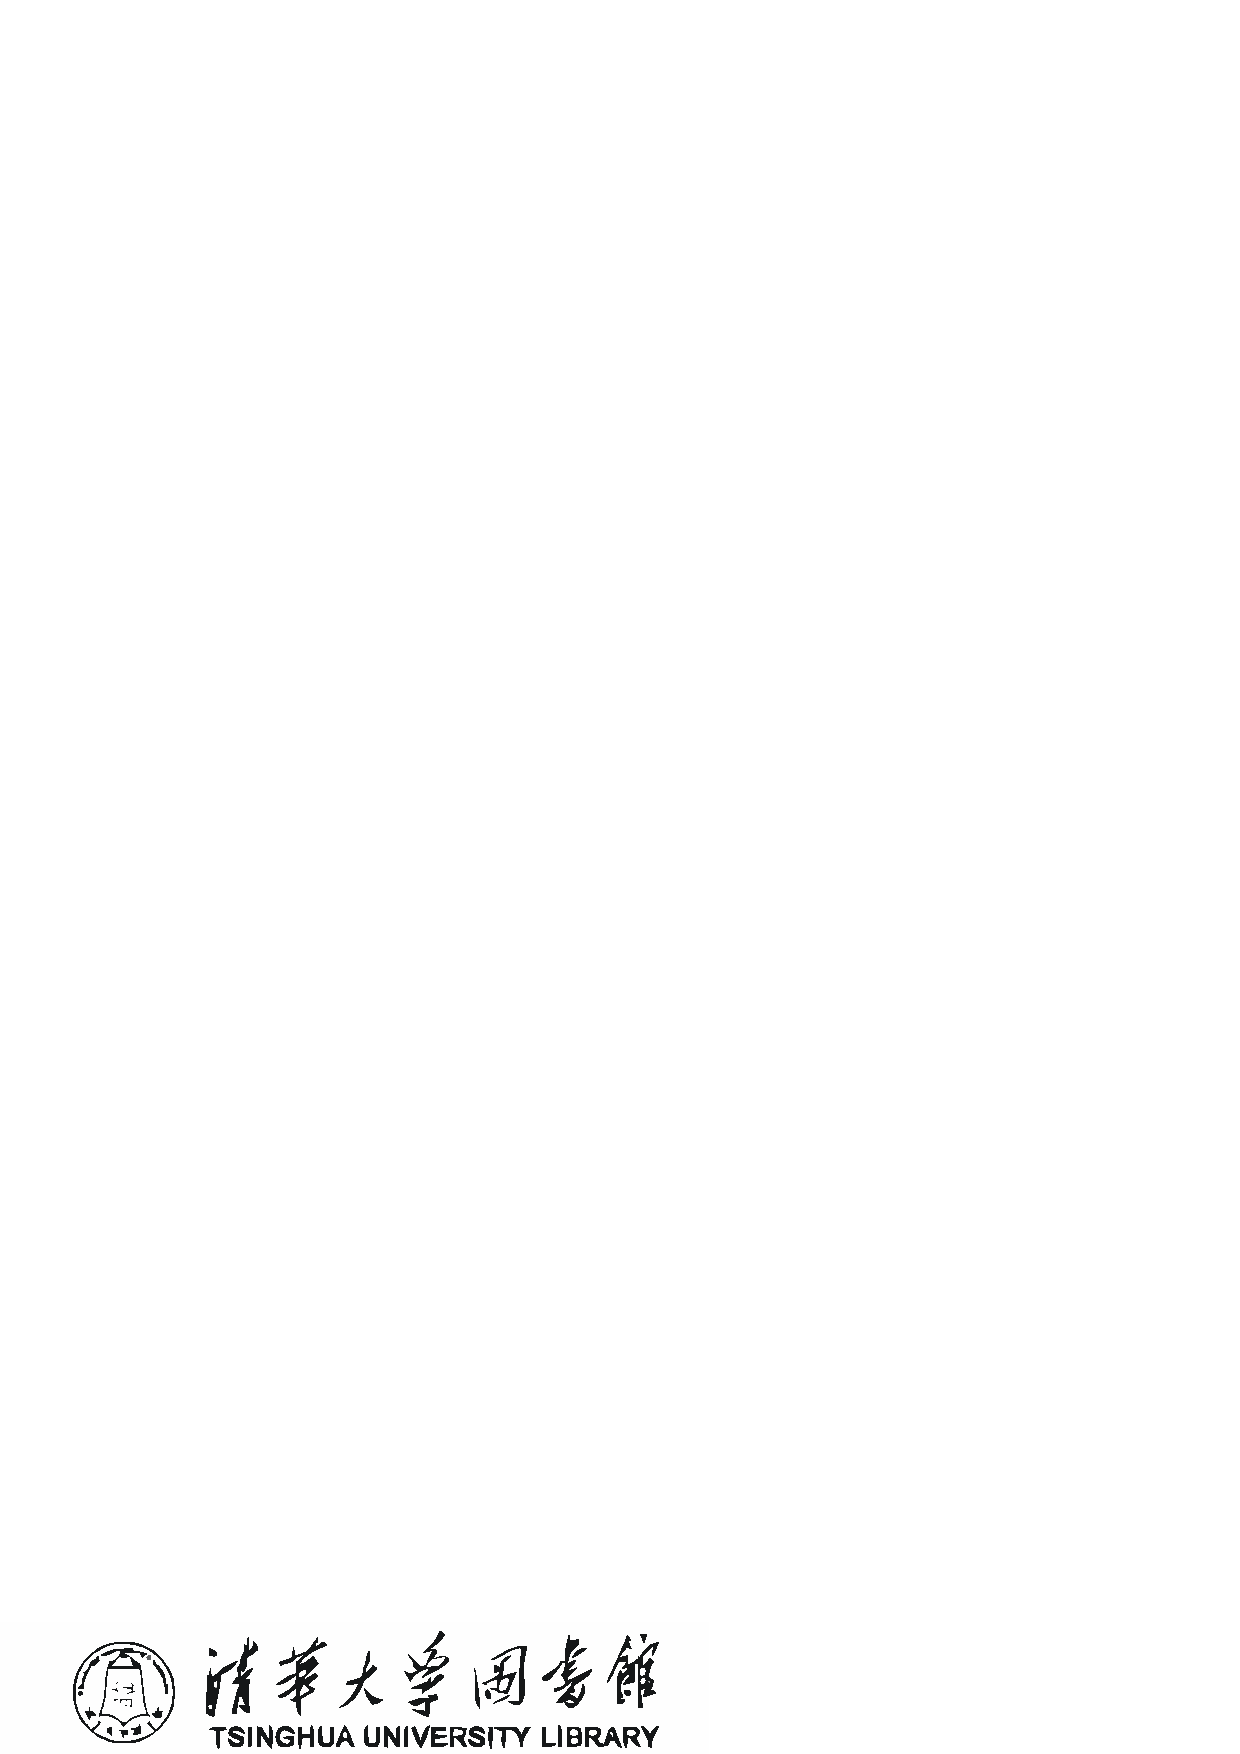
\includegraphics{thu-lib-logo}
  \caption*{Figure~1\quad This is an example for manually numbered figure,
    which would not appear in the list of figures}
  \label{tab:badfigure2}
\end{figure}

Now we consider a nonlinear programming which is confronted solely with
maximizing a real-valued function with domain $\Re^n$.  Whether derivatives are
available or not, the usual strategy is first to select a point in $\Re^n$ which
is thought to be the most likely place where the maximum exists. If there is no
information available on which to base such a selection, a point is chosen at
random. From this first point an attempt is made to construct a sequence of
points, each of which yields an improved objective function value over its
predecessor. The next point to be added to the sequence is chosen by analyzing
the behavior of the function at the previous points. This construction continues
until some termination criterion is met. Methods based upon this strategy are
called {\em ascent methods}, which can be classified as {\em direct methods},
{\em gradient methods}, and {\em Hessian methods} according to the information
about the behavior of objective function $f$. Direct methods require only that
the function can be evaluated at each point. Gradient methods require the
evaluation of first derivatives of $f$. Hessian methods require the evaluation
of second derivatives. In fact, there is no superior method for all
problems. The efficiency of a method is very much dependent upon the objective
function.

\subsection{Integer Programming}

{\em Integer programming} is a special mathematical programming in which all of
the variables are assumed to be only integer values. When there are not only
integer variables but also conventional continuous variables, we call it {\em
  mixed integer programming}. If all the variables are assumed either 0 or 1,
then the problem is termed a {\em zero-one programming}. Although integer
programming can be solved by an {\em exhaustive enumeration} theoretically, it
is impractical to solve realistically sized integer programming problems. The
most successful algorithm so far found to solve integer programming is called
the {\em branch-and-bound enumeration} developed by Balas (1965) and Dakin
(1965). The other technique to integer programming is the {\em cutting plane
  method} developed by Gomory (1959).

\hfill\textit{Uncertain Programming\/}\quad(\textsl{BaoDing Liu, 2006.2})

\section*{References}
\noindent{\itshape NOTE: These references are only for demonstration. They are
  not real citations in the original text.}

\begin{translationbib}
\item Donald E. Knuth. The \TeX book. Addison-Wesley, 1984. ISBN: 0-201-13448-9
\item Paul W. Abrahams, Karl Berry and Kathryn A. Hargreaves. \TeX\ for the
  Impatient. Addison-Wesley, 1990. ISBN: 0-201-51375-7
\item David Salomon. The advanced \TeX book.  New York : Springer, 1995. ISBN:0-387-94556-3
\end{translationbib}

\chapter{外文资料的调研阅读报告或书面翻译}

\title{英文资料的中文标题}

{\heiti 摘要:} 本章为外文资料翻译内容。如果有摘要可以直接写上来,这部分好像没有
明确的规定。

\section{单目标规划}
北冥有鱼,其名为鲲。鲲之大,不知其几千里也。化而为鸟,其名为鹏。鹏之背,不知其几
千里也。怒而飞,其翼若垂天之云。是鸟也,海运则将徙于南冥。南冥者,天池也。
\begin{equation}\tag*{(123)}
 p(y|\mathbf{x}) = \frac{p(\mathbf{x},y)}{p(\mathbf{x})}=
\frac{p(\mathbf{x}|y)p(y)}{p(\mathbf{x})}
\end{equation}

吾生也有涯,而知也无涯。以有涯随无涯,殆已!已而为知者,殆而已矣!为善无近名,为
恶无近刑,缘督以为经,可以保身,可以全生,可以养亲,可以尽年。

\subsection{线性规划}
庖丁为文惠君解牛,手之所触,肩之所倚,足之所履,膝之所倚,砉然响然,奏刀騞然,莫
不中音,合于桑林之舞,乃中经首之会。
\begin{table}[ht]
\centering
  \centering
  \caption*{表~1\hskip1em 这是手动编号但不出现在索引中的一个表格例子}
  \label{tab:badtabular3}
  \begin{tabular}[c]{|m{1.5cm}|c|c|c|c|c|c|}\hline
    \multicolumn{2}{|c|}{Network Topology} & \# of nodes &
    \multicolumn{3}{c|}{\# of clients} & Server \\\hline
    GT-ITM & Waxman Transit-Stub & 600 &
    \multirow{2}{2em}{2\%}&
    \multirow{2}{2em}{10\%}&
    \multirow{2}{2em}{50\%}&
    \multirow{2}{1.2in}{Max. Connectivity}\\\cline{1-3}
    \multicolumn{2}{|c|}{Inet-2.1} & 6000 & & & &\\\hline
    \multirow{2}{1.5cm}{Xue} & Rui  & Ni &\multicolumn{4}{c|}{\multirow{2}*{\thuthesis}}\\\cline{2-3}
    & \multicolumn{2}{c|}{ABCDEF} &\multicolumn{4}{c|}{} \\\hline
\end{tabular}
\end{table}

文惠君曰:“嘻,善哉!技盖至此乎?”庖丁释刀对曰:“臣之所好者道也,进乎技矣。始臣之
解牛之时,所见无非全牛者;三年之后,未尝见全牛也;方今之时,臣以神遇而不以目视,
官知止而神欲行。依乎天理,批大郤,导大窾,因其固然。技经肯綮之未尝,而况大坬乎!
良庖岁更刀,割也;族庖月更刀,折也;今臣之刀十九年矣,所解数千牛矣,而刀刃若新发
于硎。彼节者有间而刀刃者无厚,以无厚入有间,恢恢乎其于游刃必有余地矣。是以十九年
而刀刃若新发于硎。虽然,每至于族,吾见其难为,怵然为戒,视为止,行为迟,动刀甚微,
謋然已解,如土委地。提刀而立,为之而四顾,为之踌躇满志,善刀而藏之。”

文惠君曰:“善哉!吾闻庖丁之言,得养生焉。”


\subsection{非线性规划}
孔子与柳下季为友,柳下季之弟名曰盗跖。盗跖从卒九千人,横行天下,侵暴诸侯。穴室枢
户,驱人牛马,取人妇女。贪得忘亲,不顾父母兄弟,不祭先祖。所过之邑,大国守城,小
国入保,万民苦之。孔子谓柳下季曰:“夫为人父者,必能诏其子;为人兄者,必能教其弟。
若父不能诏其子,兄不能教其弟,则无贵父子兄弟之亲矣。今先生,世之才士也,弟为盗
跖,为天下害,而弗能教也,丘窃为先生羞之。丘请为先生往说之。”
\begin{figure}[h]
  \centering
  
\includegraphics{thu-whole-logo}
  \caption*{图~1\hskip1em 这是手动编号但不出现索引中的图片的例子}
  \label{tab:badfigure3}
\end{figure}

柳下季曰:“先生言为人父者必能诏其子,为人兄者必能教其弟,若子不听父之诏,弟不受
兄之教,虽今先生之辩,将奈之何哉?且跖之为人也,心如涌泉,意如飘风,强足以距敌,
辩足以饰非。顺其心则喜,逆其心则怒,易辱人以言。先生必无往。”

孔子不听,颜回为驭,子贡为右,往见盗跖。

\subsection{整数规划}
盗跖乃方休卒徒大山之阳,脍人肝而餔之。孔子下车而前,见谒者曰:“鲁人孔丘,闻将军
高义,敬再拜谒者。”谒者入通。盗跖闻之大怒,目如明星,发上指冠,曰:“此夫鲁国之
巧伪人孔丘非邪?为我告之:尔作言造语,妄称文、武,冠枝木之冠,带死牛之胁,多辞缪
说,不耕而食,不织而衣,摇唇鼓舌,擅生是非,以迷天下之主,使天下学士不反其本,妄
作孝弟,而侥幸于封侯富贵者也。子之罪大极重,疾走归!不然,我将以子肝益昼餔之膳。”


\chapter{其它附录}
前面两个附录主要是给本科生做例子。其它附录的内容可以放到这里,当然如果你愿意,可
以把这部分也放到独立的文件中,然后将其 \cs{input} 到主文件中。

% \end{appendix}

%% 个人简历
%\begin{resume}

  \resumeitem{个人简历}

  1991 年 03 月 01 日出生于 河北 邢台 市。

  2008 年 9 月考入 河北工业 大学  电气工程 系 电气工程及其自动化 专业,2012 年 6 月本科毕业并获得 工学 学士学位。

  2012 年 8 月免试进入 清华 大学 高等研究院 攻读 博士 学位至今。

  \researchitem{在学期间发表的学术论文} % 发表的和录用的合在一起
\noindent 1. 已经刊载的学术论文%(本人是第一作者,或者导师为第一作者本人是第二作者)

  \begin{publications}
  \item Xiaokai Huo, Wen-An Yong. Global existence for viscoelastic fluids with infinite Weissenberg number. Communications in Mathematical Sciences, 2017, 15(4): 1129-1140.(SCI收录)
  \item Xiaokai Huo, Wen-An Yong. Structural stability of a 1D compressible viscoelastic fluid model. Journal of Differential Equations, 2016, 261(2): 1264-1284.(SCI收录)
  \item Xiaokai Huo, Weitao Sun, et al. Coupling analysis of low-speed multiphase flow and high-frequency electromagnetic field in a complex pipeline structure. Mathematical Problems in Engineering, 2014(3):1-9.(SCI收录)
  \end{publications}

%  \noindent 2. 已经接收的学术论文%(本人是第一作者,或者导师为第一作者本人是第二作者)

 % \begin{publications}
%  \item Xiaokai Huo, Wen-An Yong. Global existence for viscoelastic fluids with infinite Weissenberg number. Communications in Mathematical Sciences, 2017, 15(229).(SCI收录)
  %\end{publications}

\end{resume}

\end{document}
